\documentclass[12pt]{article}
\usepackage{amsmath}
\usepackage{graphicx, color}
\usepackage{amssymb}
\usepackage{listings} %source code listing
\usepackage{multirow}
%\usepackage[version=2]{mhchem}
\usepackage{subfig}
\usepackage{tabularx}
\usepackage{hyperref}
\usepackage{units}
\usepackage{gensymb}
\usepackage{adjustbox}
\usepackage{tcolorbox}
\usepackage{listings}
\usepackage{color}
 
\definecolor{codegreen}{rgb}{0,0.6,0}
\definecolor{codegray}{rgb}{0.5,0.5,0.5}
\definecolor{codepurple}{rgb}{0.58,0,0.82}
\definecolor{backcolour}{rgb}{0.95,0.95,0.92}

\newcommand{\specialcell}[2][c]{%
  \begin{tabular}[#1]{@{}c@{}}#2\end{tabular}}
 


\title{Reactor physics with Python \\ Lecture Notes}


\author{Zs.~Elter. E. Branger, M. Preston \\ Uppsala University \\
        Division of Applied Nuclear Physics}%\corref{cja}}
%
\begin{document}

\maketitle

\newpage

\tableofcontents

\newpage

%\documentclass[12pt]{article}
%\usepackage{amsmath}
%\usepackage{graphicx, color}
%\usepackage{amssymb}
%\usepackage{listings} %source code listing
%\usepackage{multirow}
%%\usepackage[version=2]{mhchem}
%\usepackage{subfig}
%\usepackage{hyperref}
%\usepackage{units}
%\usepackage{gensymb}
%\usepackage{adjustbox}
%\usepackage{listings}
%\usepackage{color}
%\usepackage{tcolorbox}
%\usepackage{tabularx}
%\definecolor{codegreen}{rgb}{0,0.6,0}
%\definecolor{codegray}{rgb}{0.5,0.5,0.5}
%\definecolor{codepurple}{rgb}{0.58,0,0.82}
%\definecolor{backcolour}{rgb}{0.95,0.95,0.92}
%
%\newcommand{\specialcell}[2][c]{%
%  \begin{tabular}[#1]{@{}c@{}}#2\end{tabular}}
% 
%
%
%\title{Reactor physics with Python \\ Lecture Notes}
%
%
%\author{Zs.~Elter. E. Branger, M. Preston \\ Uppsala University \\
%        Division of Applied Nuclear Physics}%\corref{cja}}
%%
%\date{2021.}
%\begin{document}

\section{Introduction}

Nuclear reactors play an important role in our modern society. In some countries, such as France  the major part of electricity is produced from nuclear power. Over the last decades, we have gathered a great deal of knowledge and experience in designing nuclear reactors, but we must remember that nuclear reactors are very complex, therefore it is important to sustain this knowledge, and train professionals with the necessary understanding to operate or build new reactors. This lecture note is intended for students and professional with a basic understanding of nuclear power generation, but with no prior or little knowledge of nuclear reactor physics, who either want to gain a basic understanding of the principles of nuclear reactor theory or are motivated to follow more advanced studies in the future.

The complexity of nuclear reactors arises from the fact that there are several phenomena happening in a nuclear reactor at different scales, which interplay: heat production from nuclear fission, heat transfer and fluid dynamics. In some context reactor physics can refer to all of these phenomena, however traditionally reactor physics is meant to be limited to describing the physics within the reactor core, where the nuclear fuel and the coolant can be found and intends to describe the transport of neutrons within the core. This text is also limited to studying the reactor core, and it intends to provide an introductory, often phenomenological description to convey the main concepts, and to serve as a good basis for future advanced studies. Figure \ref{fig:reactorcore} stand here to highlight that indeed from the whole system of a nuclear power plant, our interest is during the text only the neutron physics happening inside the reactor vessel: within the nuclear fuel, the coolant material and the control elements. 

The aim of this lecture note and the related datalab exercises is to teach through (hopefully) pedagogical examples which can be implemented as small programs. It is however important to highlight that this text is a \textit{lecture note}, it does not intend to cover everything and include every important derivation, only the ones said during the lectures. The note had two intentions: to provide scientific figures created with python, so the students can have access to the source code of the figures and to give a summary of the lectures in order to aid the lecturer during teaching. However a student reading this text will need to review further literature to grasp the subject. The following books can provide great help:

\begin{itemize}
\item Duderstadt, James J.: Nuclear reactor analysis (referred to as D\&H during the note)
\item Lewis, E. E.: Fundamentals of nuclear reactor physics
\item Lamarsh, John R.: Introduction to Nuclear Reactor theory
\item Bell, George and Glasstone, Samuel: Nuclear Reactor Theory (referred to as B\&G during the note)
\item W. Stacey: Nuclear reactor physics
\item C. Demaziere: Physics of nuclear reactors (lecture notes)
\item Z. Szatmary: Introduction to reactor physics (although only for Hungarian speakers)
\end{itemize}

In fact during the writing of these notes we have heavily relied on these books. Mostly we have tried to follow D\& H, but we have used other books, where they provided a more illustrative explanation or derivation. Some parts of these lecture notes will therefore show some similarities to these books. We will however not include a reference for every single equation in the notes, nevertheless at some point we will point out the right book for further reading.

\subsection{Nuclear reactors}

As we said earlier the reader of these notes is expected to have a basic familiarity of nuclear plants and reactors. If that is not the case, please read for example D\& H Chapter 3-II, here we just provide a brief introduction to introduce the terminology used in this text.

\begin{figure}[ht!]
\protect \centering{
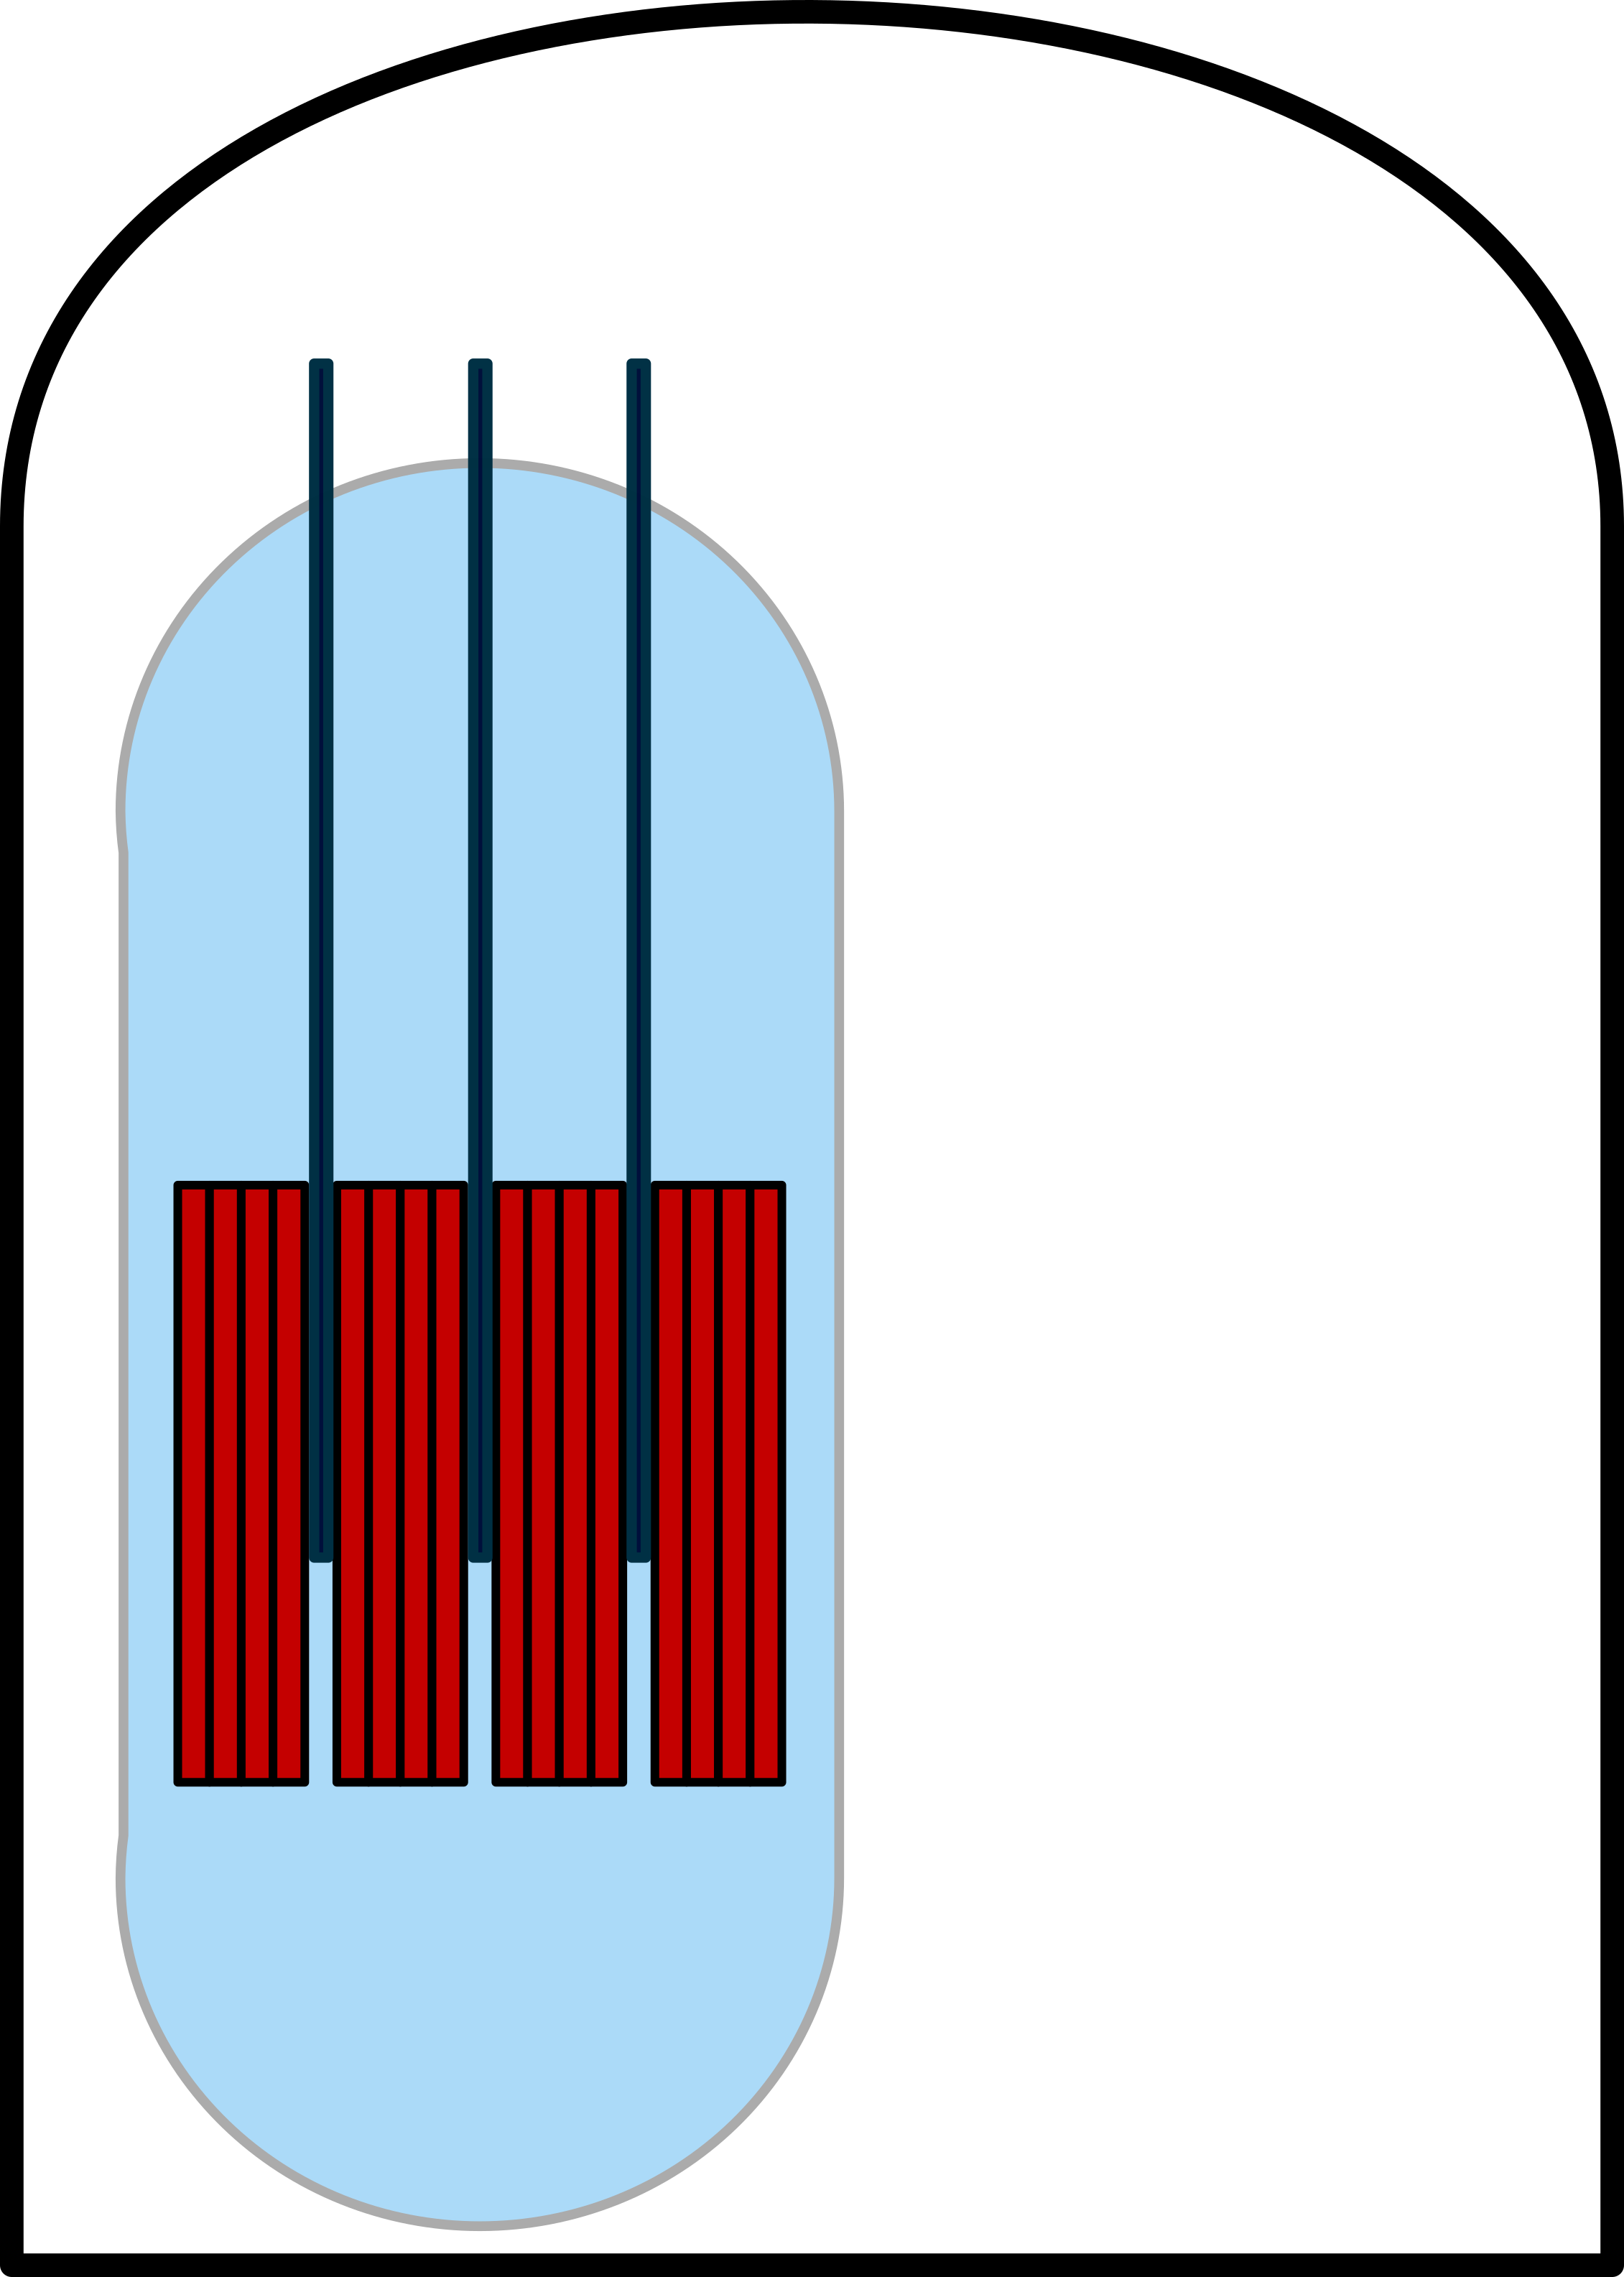
\includegraphics[scale=0.36] {figures/00-reactorofinterest.png}}\protect
\caption{\label{fig:reactorcore} \footnotesize{The part of the power plant which is of interest for the subject of this lecture note: the reactor core.}}
\end{figure}

As said earlier the focus of this text is on the heart of the nuclear power plant: the reactor core. Also, the main focus of this text is going to be Light Water Reactors (LWR), since to this reactor type is the most widespread. The reactor core of an LWR is located in a pressure vessel and is built of nuclear fuel, coolant channels, structural and control elements. Typically we also require some sort of monitoring of the core, therefore usually various instrumentation systems are placed in the core. The fuel is made of uranium in the ceramic form of uranium-dioxide (often referred to as UOX, or UO$_2$). As we will see later, the uranium might be enriched: the weight fraction of the fissile isotope uranium-235 is higher than in natural uranium. The UOX material is formed into small cylindrical \textit{pellet}s, which are placed in a metallic, often zirconium tube, the \textit{cladding}. The tube is filled usually with an inert gas, and sealed. This tube is called a \textit{fuel pin} or \textit{fuel rod}. The fuel pins are then placed in a \textit{bundle} or \textit{assembly}. Western type fuel assemblies are usually rectangular lattices, whereas eastern type assemblies have a hexagonal lattice. Figure \ref{fig:assembly} shows the layout of a 17x17 pressurized water reactor (PWR) assembly, which contains 25 control rod positions in \textit{guide tubes}. The fuel assemblies are arranged into a lattice (again depending on the type of the reactor this might be rectangular or hexagonal) which makes up the core, with a close to cylindrical shape. In some reactors the core is surrounded by non-fuel assemblies (\textit{reflectors} and \textit{shielding}), or fuel elements which have special use (for example \textit{breeding blankets}). Later we will discuss these in more detail. Table \ref{table:pwrsize} summarizes the typical sizes of a PWR reactor. 

\begin{figure}[ht!]
\protect \centering{
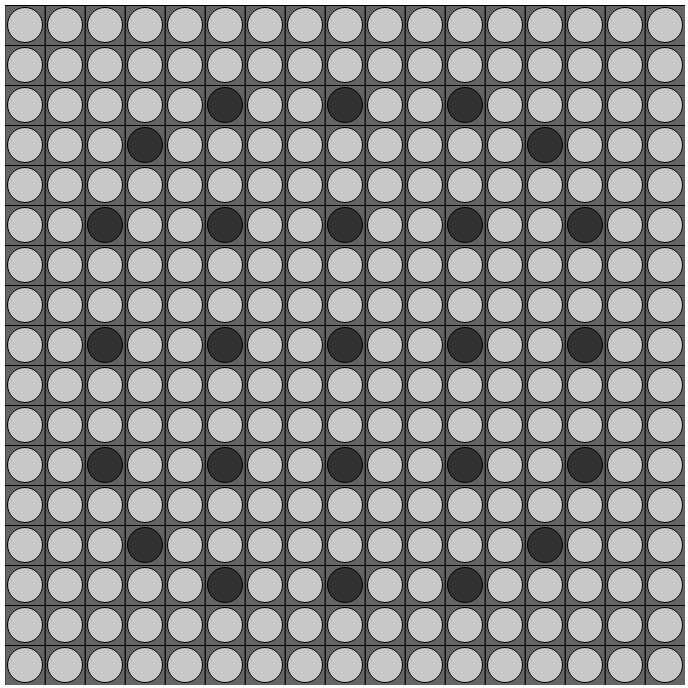
\includegraphics[scale=0.26] {figures/00-assembly.png}}\protect
\caption{\label{fig:assembly} \footnotesize{A 17x17 PWR assembly lattice (darker positions highlight the control rods).}}
\end{figure}

\begin{table}\caption{Typical size of a PWR core}\label{table:pwrsize}
\begin{tabular}{c c}
Core diameter & 3-4 meters \\
Core height & 4 meters \\
Assembly width & 20 cm \\
Pin diameter & 1.0 cm \\
Pin pitch & 1.2 cm
\end{tabular}
\end{table}


\subsection{Reactor physics}

As mentioned before, the main subject of this text is reactor physics. However, even this can be split into further parts:

\begin{itemize}
\item Neutronics: to determine the distribution of neutrons in time, in energy, and in space for a given geometry and material configuration.
\item Depletion or burnup studies: Investigate how the material composition changes in the reactor core over time: how much fissile material is lost, how much transuranic elements and fission products are created. 
\item Experimental reactor physics: Provide measurement methods which can be used to determine various quantities important during reactor operation.
\end{itemize}

In this text we will mainly focus on neutronics, and touch upon depletion. We will first introduce the relevant part of nuclear physics in order to describe reactions which might happen with neutrons traveling in a reactor. Then we will discuss how a neutron looses its kinetic energy in a nuclear reactor (this is the subject of \textit{slowing down}), and in fact at the end of its life it reaches thermal energies (this is the subject of \textit{thermalization}). Then we will derive a \textit{neutron transport} equation describing the balance between the production and loss of neutrons in the reactor. Then we will investigate how the number of neutrons changes in the reactor over time if we increase the probability of neutron survival (for example by removing control rods). And finally we will leave behind the subject of neutronics, and study how the nuclear fuel evolves due to long-term irradiation and how this affects the neutron transport.

It must however mentioned, that the book is also a good introduction to neutron physics in general, that is a large portion of the text (on basic nuclear physics, neutron slowing down and neutron transport, neutron activation) is applicable even in non-multiplying media, which has practical relevance outside of the nuclear industry.  

\subsection{History of reactor physics}

Introducing the history of a subject before the subject has always the risk that parts are not going to be clear. Nevertheless, we have decided to outline first the history of reactor physics first, because it is both exciting pedagogic to see how great minds came up with ideas which at the end let to the widespread use of nuclear reactors.

\begin{tabularx}{\textwidth}{c | X}
1895 & Wilhelm R\"ontgen discovers X-rays  while testing various types of vacuum tubes. \\
1896 & Henri  Becquerel noticed that uranium ore emits similar radiation. \\
1898 & Marie and Pierre Curie shows that in fact three types of radiation is emitted. They discover radioactivity. \\
1911 & Rutherford discovers the nucleus while investigating the scattering of alpha-rays. But the discovery makes it difficult to explain the mass of the nucleus. \\
1932 & James Chadwick discovers the neutron. He uses the reaction $\text{He-4} + \text{Be-9} \rightarrow \text{C-12} + \text{n}$. Such reaction needs energetic alpha particles. With his discovery finally the nucleus mass and beta-decay can be explained.\footnote{One might wonder why Beryllium was used in such experiments. One needed a nucleus with small charge, so $\alpha$ particles can get close. Hydrogen and Helium are gases, which makes it difficult to fabricate a target, whereas Lithium is rather dangerous to work with, therefore scientist at the time were left with Beryllium as the next candidate in the periodic system.}
 
Even more important it was discovered that the neutral particle can penetrate the nucleus therefore it became possible to convert it.  The study of nuclear reactions, modern alchemy has began (mostly with a PoBe source, where the alpha-decaying Polonium is mixed with Beryllium). \\
1934 & Frederic Joliot-Curie and Irene Curie noticed after the absorption of a neutron, a beta-decay might follow (induced radioactivity), and the element is transmuted into an other element. 
\end{tabularx}

\begin{tabularx}{\textwidth}{c | X}
1930s & Enrico Fermi's team systematically tried to transmutation reactions for several isotopes. They found that upon performing the neutron activation experiments under water, the induced radioactivity is much higher. Fermi thus started to develop the theory of neutron slowing down and found that, the initially fast neutrons scatter on the hydrogen atoms, and they reach thermal energy (when the speed is comparable to that of thermal motion). They also found that by activating uranium they can produce elements heavier than the ones existing in nature: neptunium and plutonium. \\
1938 & Fermi receives the Nobel for this work. \\
1938 & When Otto Hahn and Fritz Strassmann repeated the activation experiments of uranium they observed several beta decays, which couldn't be explained by the transuranic element. From the reaction products they managed to separate Barium. Then Lisa Meitner realized that uranium had to undergo fission, and infact it is the fission products which emit the unaccounted beta-radiation. \\
1933 & (Note that we jumped back in time!) Leo Szilard comes up with the idea of a chain reaction: if the product of neutron activation produces new neutrons these neutrons could be used for further reactions. He patented the idea of a nuclear reactor, already before he even knew about fission. He assumed that there has to be a reaction which results in a neutron which can self-sustain the reaction. And with the discovery of fission this became obvious. Also that we can produce a lot of energy in this way. 
\end{tabularx}

\begin{tabularx}{\textwidth}{c | X}
1939 & Leo Szilard becomes conscious about the possibility of building a nuclear bomb and convinces Albert Einstein to write a letter to President Roosevelt about the potential of a nuclear bomb, and the threat of Germany already developing it (after all they discovered fission). They stopped all publications on the subject. The Manhattan Project started, during which they realized that there are two ways of making such a bomb: with uranium-235 or plutonium-239. The first option needed separation from U-238 (since in nature the weight fraction of uranium-235 is low), which proved to be difficult at that time (the separation couldn't be based on chemistry, had to be based on the slight difference in mass). The second option required the neutron activation of uranium-238. To carry out such reactions at scale, a large amount of neutrons were needed, which couldn't be produced with the typical neutron sources of the time. This required a chain reactor. \\
1942 & Chicago-pile. By placing UO2 rods (made of natural uranium) in hole of graphite bricks the first controlled chain reaction was achieved. It gave a proof of concept for chain reaction and also allowed the discovery of that there are enough delayed neutrons, thus the chain reaction can be controlled. \\
1944 & The Hanford reactor was built for plutonium production. Chemical reprocessing methods were used to separate plutonium from uranium. \\
1945 & Was a sad year of reactor physics. \\
1951 & EBR-1 fast reactor was built and produced electricity. \\
1955 & Obninsk Nuclear Power Plant, first nuclear station was built and produced a whooping 6MW power.
\end{tabularx}

And then the era of nuclear power stations started, building hundreds of reactors both for energy production and for research.


\subsection{Programming with python}

Of course as the name of the course shows "with Python" is appended to reactor physics. Reactor physics in practice requires a lot of computations from numerical solutions of differential equations through handling large amount of nuclear data till processing measured results. Our experience is that the best way to learn reactor physics is by applying it in practice, therefore it was decided that the lectures will be complemented with 11 datalabs, where students can develop simple simulations of neutron transport, perform data analysis, and also use more advanced Monte Carlo codes. It was decided that students will use Python and its mainstream libraries for these tasks. The main reason is that Python has a very simple syntax, thus students can quickly learn it. Also, it was important that the simulations we will develop are intended to help the understanding of reactor physics, thus it would not have been ideal if the complexities of some programming language hindered us. We acknowledge that for advanced reactor physics, where computational efficiency and time is crucial, Python might not be the preferred choice.

Nevertheless, in this lecture note it is not going to be apparent that this course is a "python" course. The only place where Python occurs in the notes is behind the scenes: the scientific figures were created with Matplotlib, the plotting library of Python, with the aim that the source code can be distributed along the figures, to be transparent and to help understanding the data behind the figures. 

We strongly hope that students performing all the datalabs while reading the lectures will become proficient users of Python. Nevertheless, we have to emphasize that the main goal of having programming exercises during the datalabs is to help students understand the basic theory of nuclear reactors and neutron transport.

%\end{document}

%\documentclass[12pt]{article}
%\usepackage{amsmath}
%\usepackage{graphicx, color}
%\usepackage{amssymb}
%\usepackage{listings} %source code listing
%\usepackage{multirow}
%%\usepackage[version=2]{mhchem}
%\usepackage{subfig}
%\usepackage{hyperref}
%\usepackage{units}
%\usepackage{gensymb}
%\usepackage{adjustbox}
%\usepackage{listings}
%\usepackage{color}
%\usepackage{tcolorbox}
% 
%\definecolor{codegreen}{rgb}{0,0.6,0}
%\definecolor{codegray}{rgb}{0.5,0.5,0.5}
%\definecolor{codepurple}{rgb}{0.58,0,0.82}
%\definecolor{backcolour}{rgb}{0.95,0.95,0.92}
%
%\newcommand{\specialcell}[2][c]{%
%  \begin{tabular}[#1]{@{}c@{}}#2\end{tabular}}
% 
%
%
%\title{Reactor physics with Python \\ Lecture Notes}
%
%
%\author{Zs.~Elter. E. Branger, M. Preston \\ Uppsala University \\
%        Division of Applied Nuclear Physics}%\corref{cja}}
%%
%\date{2021.}
%\begin{document}

\section{Basics of Nuclear Physics}

The main purpose of building nuclear reactors is to extract the energy from nuclear fission events. In fission events heavy nuclei split into two or more lighter nuclei followed by the release of energy and radiation. Fission can occur spontaneously, however for most nuclides this is a rare event. An other possibility is to induce fission, and the most practical approach is to bombard the nucleus with a neutral particle which doesn't feel the electric charge of the nucleus. Therefore, most of the currently operating nuclear reactors utilize the neutron induced fission of uranium-235 and of other fissile nuclides (eg. plutonium-239):

\[
\text{neutron}+{}^{235}\text{U} \rightarrow \text{fission products} + \text{neutron(s)} + \text{energy}
\]

From this reaction energy is released in the form of kinetic energy of the products (which heats up the surrounding by bouncing on other atoms) and radiation. It is also apparent that the neutrons emerging from the reaction can induce further fission events, hence it is possible to sustain a chain reaction in the reactor core. Neutrons may however enter reactions other than fission, or leave the reactor core without participating in any reaction relevant to the chain reaction within the core. Therefore, it is important to balance the number of neutrons initiating fission events and the number of neutrons lost for the chain reaction. Designing the neutron economy of a nuclear reactor is one of the primary subjects of nuclear reactor physics or neutronics. 

In order to study the neutron induced chain reaction in a given reactor core we have to understand the physics of nuclear reactions. Since in most of the reactor cores there is a large number of neutrons (10-100 millions per cm${}^3$), usually the description of the average behavior of neutrons is adequate. Thus we will deterministic equations to describe the neutron population of the system. We will however see the most accurate study can performed with a stochastic approach based on Monte Carlo particle transport methods. Nevertheless, both of these approaches require the knowledge of the probabilities of neutron-nuclear reactions occurring, which is a subject of nuclear physics

Hence it is impossible to avoid reviewing the basics of nuclear physics which are relevant to reactor physics. This section is just a brief review of the subject, cherry picking the most important concepts of nuclear reactions. The two types of such reactions are spontaneous  disintegration processes (ie. radioactive decay) and collision reactions.  As we will see later both type of reactions have an important role in the behavior of reactor cores. 

Nevertheless, some of these concepts provide an excellent opportunity to write simple data analysis scripts and programs in Python.

\subsection{Nuclides and the binding energy}

An atom is made of a nucleus and electrons zooming around the nucleus. And the atomic nucleus is made of protons and neutrons. The number of protons is denoted by the atomic number $Z$, or by the chemical symbol. The proton number usually influences what chemical reactions the atom will enter. The number of neutrons is denoted by $N$, and the sum of the neutron and proton number is the mass number $A=N+Z$. The various neutron-proton configurations are called nuclides, and the nuclei having the same number of protons but different number of neutrons is called an isotope. 

Generally we will refer to nuclides as ${}_Z^A\text{X}$ or simply ${}^A\text{X}$ since the element symbol already describes the proton number. Sometimes you might even find the notation $\text{X}\text{A}$. (Eg. ${}_{94}^{239}\text{Pu}$, ${}^{239}\text{Pu}$, $\text{Pu}239$).

Nuclei can be in excited states referred to as ${}_Z^A\text{X}^*$. When the excited state is long lived (more than the fraction of seconds), we refer to them as metastable states~${}_Z^{Am}\text{X}$.

There is an attractive force between nucleons in the nucleus, which keeps them together. This force presents an associated potential energy. Therefore, the separation of the nucleons from each other requires energy. This energy is called the binding energy ($BE=|E_p|=\int\limits_{-\infty}^\infty Fdr$). Due to this the energy of the nucleus is less then the energy of its constituent nucleons. And this is also true for the mass. 

\[
M(A,Z)<Nm_n+Zm_p
\]

\noindent where $M(A,Z)$ is the mass of the nucleus, $m_p$ and $m_n$ is the mass of the proton and the neutron. In fact the mass defect can be used to define the binding energy:

\[
BE=\Delta mc^2=[Nm_n+Zm_p-M(A,Z)]c^2
\]

One has to notice that this mass defect is not unique to the nuclear force, however the nuclear force is large enough that the defect is not negligible (MeV whereas for eg. the electronic binding the energy is in the order of electron volts).

We can then calculate the average binding energy per nucleon:

\[
\epsilon=\frac{BE}{A}=\frac{1}{A}[Nm_n+Zm_p-M(A,Z)]c^2
\]

Figure \ref{fig:binding} shows the average binding energy for some nuclides. We can notice that the ${}^4$He is a more tightly bond system than the nuclides around it (see later $\alpha$-decay). Also we can notice that the curve has a maximum at ${}^{62}$Ni\footnote{Some textbooks note that iron-56 is the most stable nuclide and it has the highest binding energy per nucleon. The second half of this statement is a common misconception. The first part is might be true. For more information: \url{https://nuclidecalendar.github.io/days/dec16.html}}. We can already notice at this point that by splitting heavier nuclei, or by fusioning lighter nuclei we can release energy.


\begin{figure}[ht!]
\protect \centering{
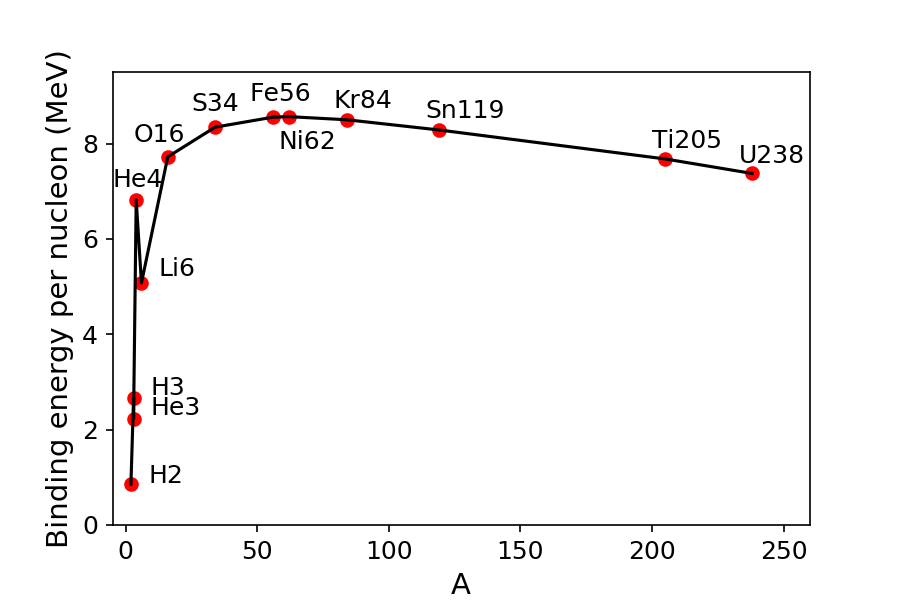
\includegraphics[scale=0.56] {figures/01-bindingcurve.png}}\protect
\caption{\label{fig:binding} \footnotesize{Binding energy per nucleon for selected nuclides. ${}^{62}\text{Ni}$ is the most bounded nuclide.}}
\end{figure}


The average binding energy can be approximated with the semi-empirical Bethe–Weizs\"acker formula, which is based on the liquid drop model of the nucleus and has various, similar forms in literature with slightly different values. Here we use one from [Anglart]

\begin{equation}
BE(A,Z)=15.75A-17.8A^{2/3}-94.8\frac{(A/2 - Z)^2}{A}-0.71Z^2A^{-1/3}+34\delta A^{-3/4}
\end{equation}

where $\delta = 1$ for even-even nuclei, $\delta = -1$ for odd-odd nuclei and $\delta = 0$ otherwise. The constants are in MeV. The relevance of this formula is that it gives some heuristic explanation of the binding energy.

\begin{itemize}
\item 1st, volume term: inside the "drop" all nucleons have more neighbors, therefore it is bonded to more nucleons. If all nucleons would be inside the drop they would feel the force of all other nucleons, therefore the binding energy would increase with $\propto A$
\item 2nd: surface term: nucleons on the surface will have less neighbors, therefore they experience lower binding energy. The number of such nucleons is proportional to the surface $\propto R^2=A^{2/3}$
\item 3rd: Symmetry term: due to the Pauli principle one energy level can be occupied only by two particles (with different spins), thus a different number of neutrons and protons result in excess energy. In fact if there was not the repulsive interaction of protons, ideally a nucleon would have the same number of protons and neutrons. The number of neutrons occupying higher levels than the protons is $N-Z$, and also the amount of excess energy of neutrons is proportional to $N-Z$. And the distance of the energy levels is $\propto 1/A$. For further explanation see [John Lilley: Nuclear Physics]. In total this energy is $\propto (N-Z)^2=(A-2Z)^2$. 
\item 4th, Coulomb term: protons will repel each other due to having the same electric charge $\propto \frac{Z^2}{R}=Z^2A^{-1/3}$
\item 5th, pairing term: Empirical observations show that nuclei having even number of protons or neutrons are more stable, especially if both are even. The reason is that similar nucleons like to be in pairs (this cannot be explained by the liquid drop model. 
\end{itemize}
 

\subsection{Nuclear reactions}

As said before there are two type of nuclear reactions important in the context of reactor physics:

\begin{itemize}
\item Spontaneous disintegration reactions (ie. decay reactions)
\item Collision reactions
\end{itemize}

\subsubsection{Decay reactions}

In decay processes the nucleus undergoes a transformation spontaneously  which results in the creation of an other nuclide. The process is accompanied by the emission of particles. The most common decay processes in nature are:

\begin{itemize}
\item $\alpha$-decay: a He nucleus is emitted for heavier nuclides (when the repulsive Coulomb force overcomes the attractive nuclear force)  ${}_Z^A\text{X} \rightarrow {}_{Z-2}^{A-4}\text{Y} + {}_2^4\text{He} + Q$.
\item $\beta^-$-decay: a neutron in the nucleus is transformed into a proton and an electron: ${}_Z^A\text{X} \rightarrow {}_{Z+1}^{A}\text{Y} + e^-+\bar\nu_e + Q$
\item $\beta^+$-decay: a proton in the nucleus is transformed into a neutron and a positron: ${}_Z^A\text{X} \rightarrow {}_{Z-1}^{A}\text{Y} + e^{+}+\nu_e + Q$
\item $\gamma$-decay: when the nucleus is in an excited state it can release energy in the form of $\gamma$ photons to reach a lower energy level or the ground state. The energy of the gamma photons is characteristic to the nuclide. ${}_Z^A\text{X}^*\rightarrow {}_Z^A\text{X} + \gamma$
\item neutron emission: as we will see later in the course some nuclides emit a neutron following a $\beta$-decay. This process has a great importance in reactor physics.
\end{itemize}

\noindent in the decay some energy in the form of kinetic energy ($Q$) is released. The released energy can be calculated from the binding energy of the original nuclide and the products.

\begin{tcolorbox}
Exercise

$${}_{88}^{226}\text{Ra}\rightarrow {}_{86}^{222}\text{Rn}+{}_{2}^{4}\text{He}$$

The binding energies (in the datalab we will calculate the $\epsilon$ average binding energies

$BE({}_{88}^{226}\text{Ra})=7.66196\cdot 226=1731.60296 \: MeV$

$BE({}_{86}^{222}\text{Rn})=7.69449\cdot 222=1708.17678 \: MeV$

$BE({}_{2}^{4}\text{He})=7.073922\cdot 4=28.295688 \: MeV$

Thus the total energy released

$$Q=[BE({}_{86}^{222}\text{Rn})+BE({}_{2}^{4}\text{He})]-BE({}_{88}^{226}\text{Ra})=4.8695 \: MeV$$

which is an enormous amount of energy. Let's consider that 1kg of ${}_{88}^{226}\text{Ra}$ decays. The number of nuclei is

$N=\frac{mN_A}{M}=2.6\cdot 10^{24}$

\noindent where $N_A$ stands for Avogadro's number, thus the total released energy would be

$E=NQ=2028 \: GJ$

Of course as we will see soon, this energy is released over thousands of years.
\end{tcolorbox}



\begin{figure}[ht!]
\protect \centering{
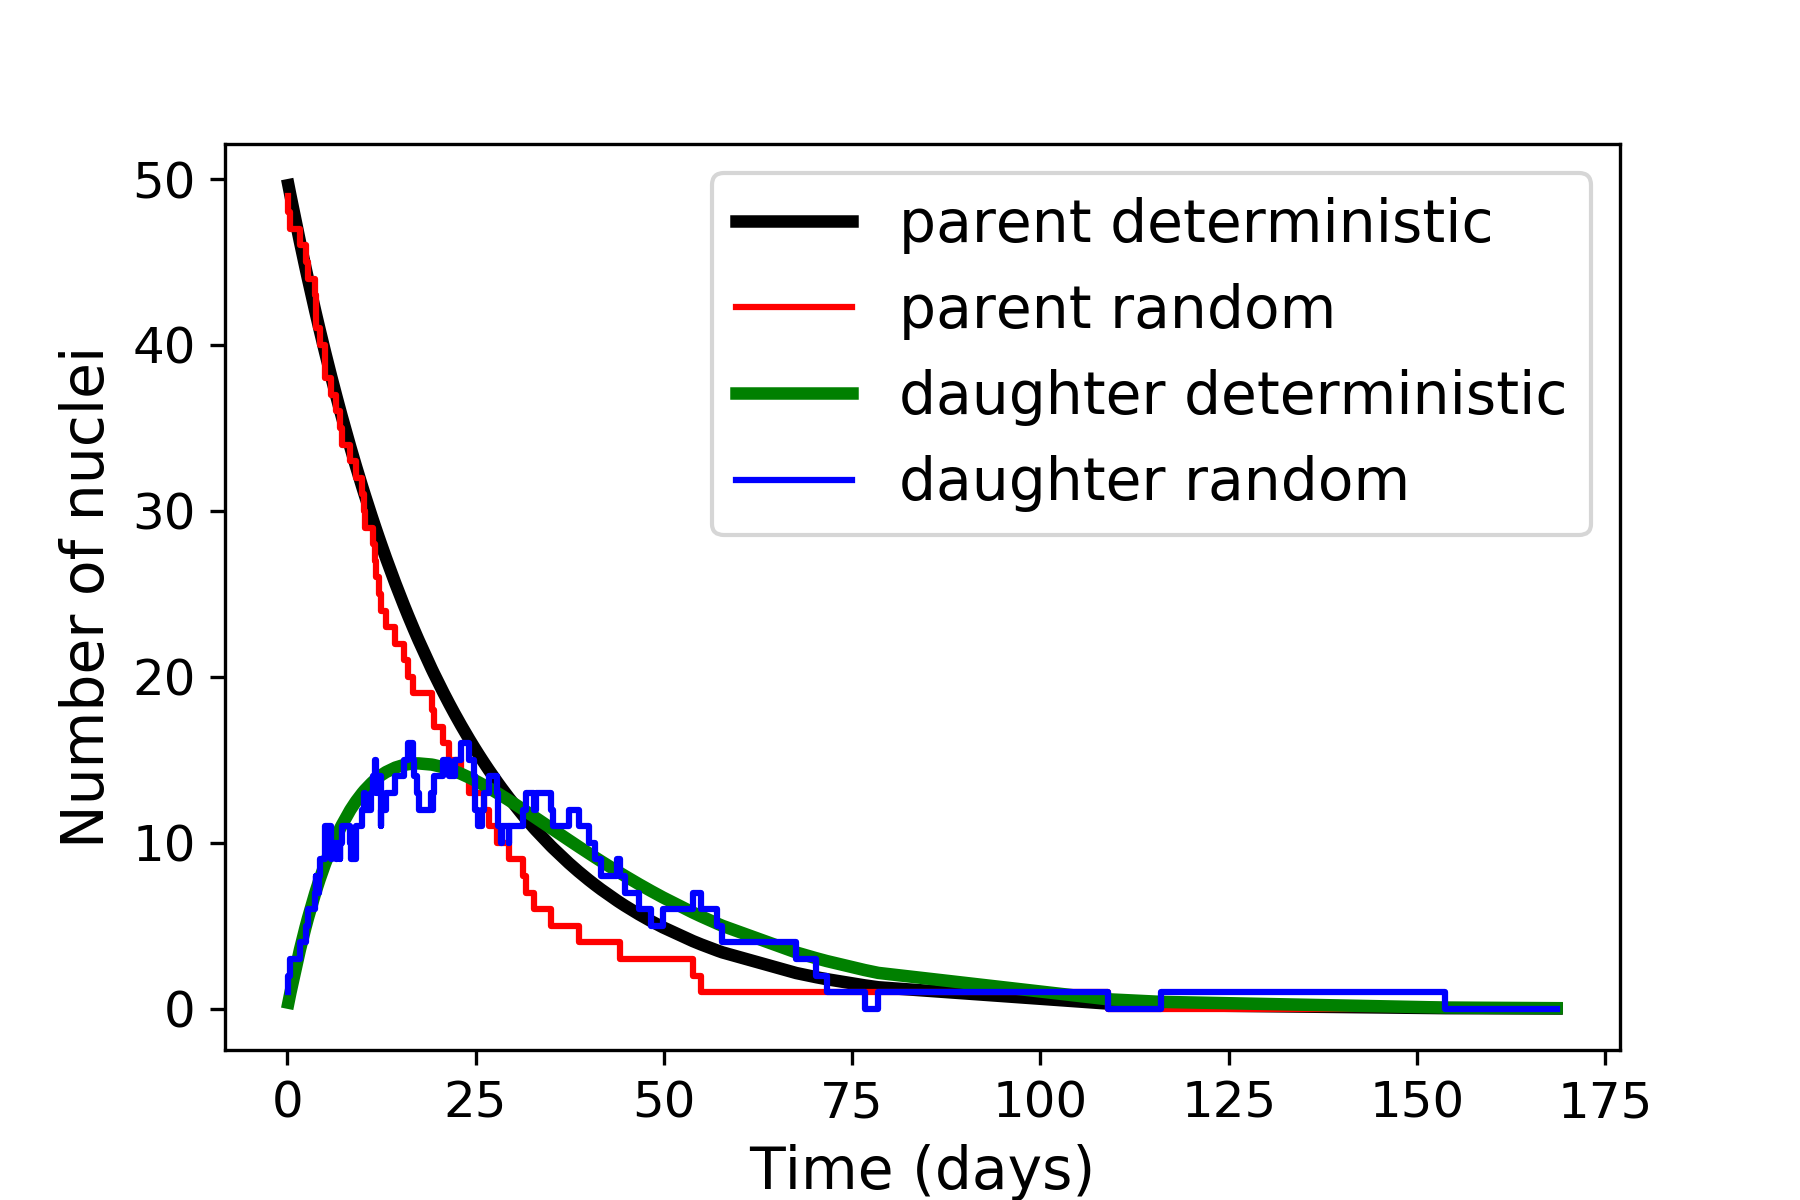
\includegraphics[scale=0.46] {figures/01-radioactivdecay_daughterparent.png}
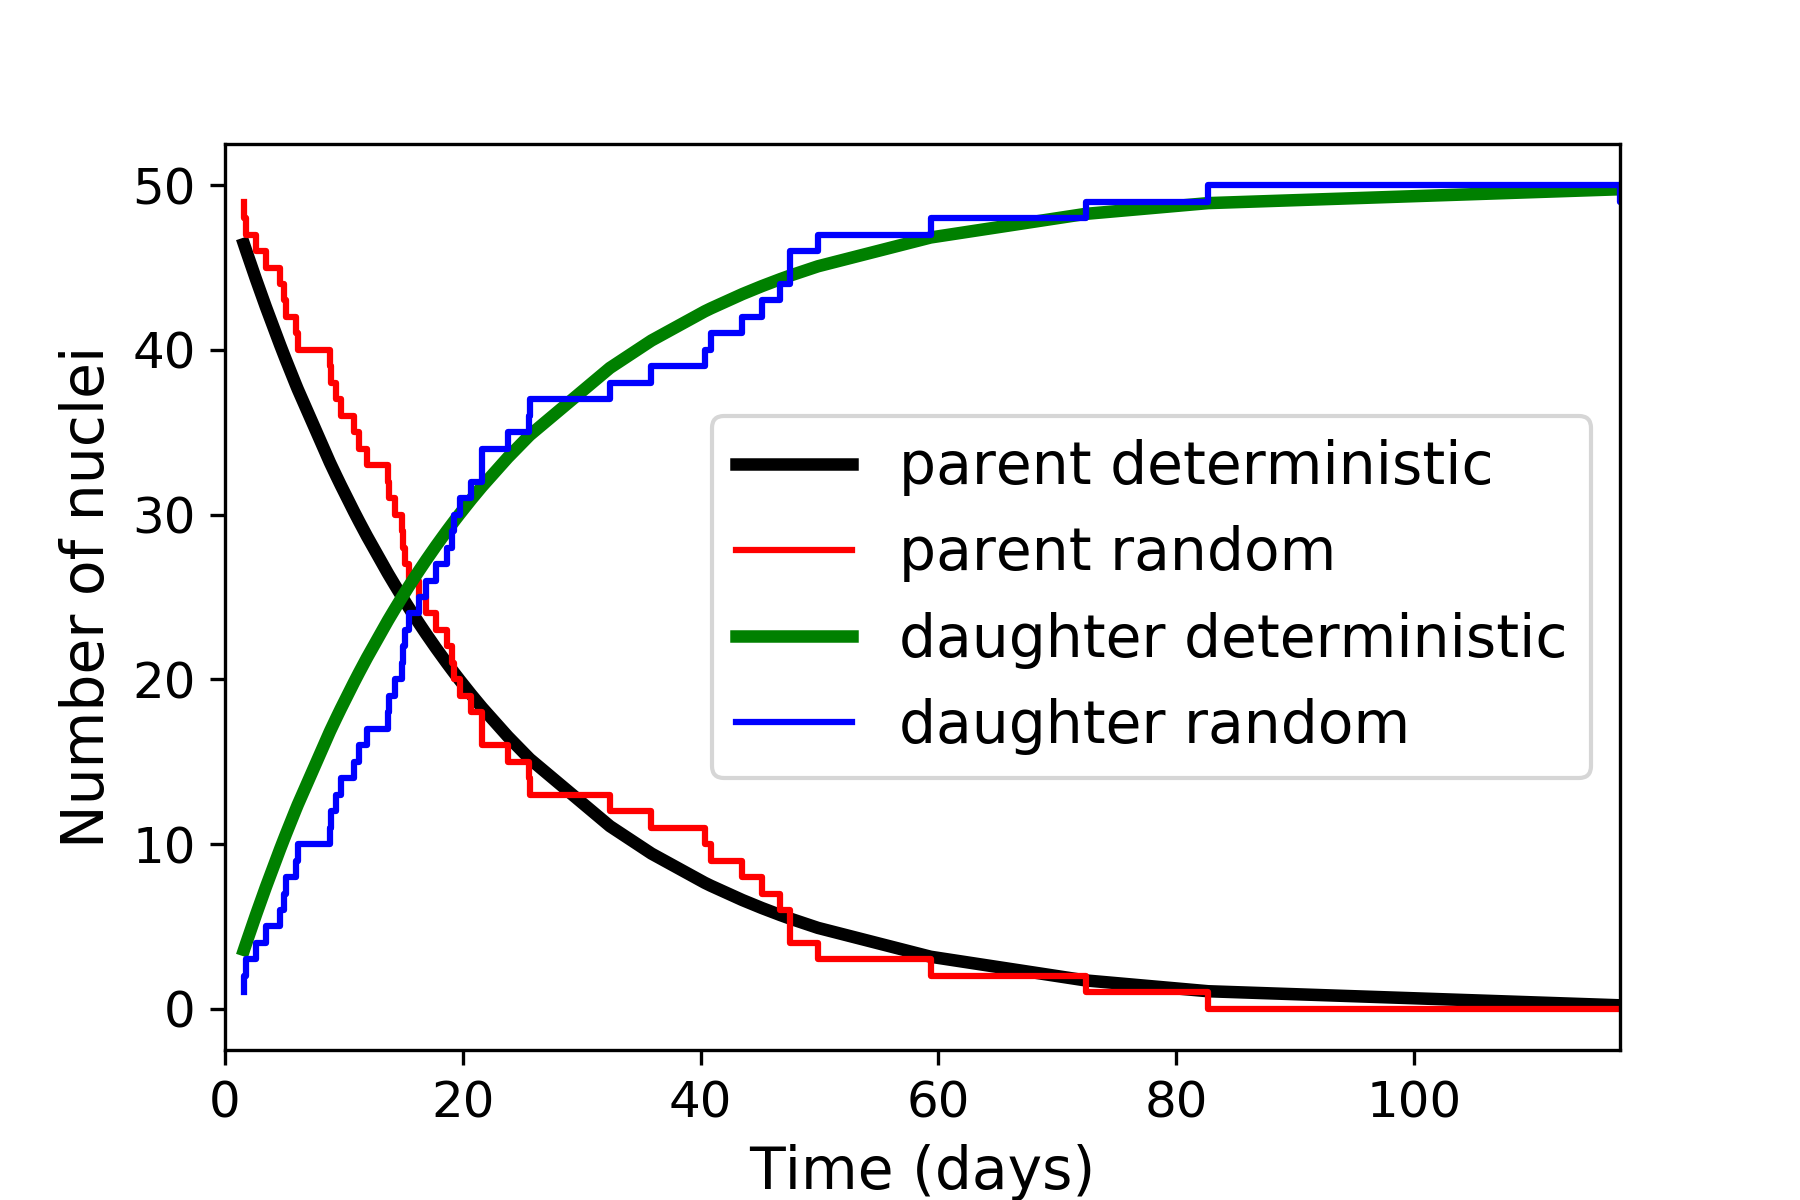
\includegraphics[scale=0.46] {figures/01-radioactivdecay_daughterparent_LongDaughter.png}}\protect
\caption{\label{fig:decay} \footnotesize{Decay of parent and daughter nuclide (Random notes a case when the decay times are sampled from an exponential distribution). Top: $T_{1/2,P} > T_{1/2,D}$. Bottom	: $T_{1/2,P} << T_{1/2,D}$}}
\end{figure}

The fundamental law of decay is that (based on observations) the probability of the decay of a nucleus in a given time interval is constant. This means that the chance to decay does not depend on the age of the nucleus. In other words, if we have more nuclei, the rate of decays (or the change in the number of nuclei in time) is proportional to the number of nuclei:

\begin{equation}
\frac{dN}{dt}=-\lambda N(t)
\end{equation}

\noindent where the decay constant $\lambda \: [s^{-1}]$ is characteristic to the type of nuclide and where $N(t)$ is the number of nuclei. However often it is more practical to write up such equation for the number density (in $\#/cm^3$). The solution to this equation is

\begin{equation}\label{eq:decay}
N(t)=N_0e^{-\lambda t}
\end{equation}

\noindent with some initial number of nuclei (or number density) $N_0=N(t=0)$. Therefore rate or as often called the activity is

\begin{equation}
\text{Rate}=A(t)=\lambda N(t)=\lambda N_0e^{-\lambda t}
\end{equation}

The activity has its units in $s^{-1}=Bq$, however in some older texts one can encounter the unit $Ci=3.7 \cdot 10^{10}\: Bq$. The $Ci$ is defined so that $1 \: Ci$ is the activity of 1g of Radium. We can clearly see that the activity of a sample depends both on the type of nuclides in the sample (due to the decay constant) and also on the quantity of radionuclides in the sample.

Although these equations are deterministic, however as said before radioactive decay is a stochastic process. An other way to interpret these equations is to consider that the probability of decay during the time interval $(t,t+dt)$ for a given nucleus is

\begin{equation}
p(t)dt=\lambda e^{-\lambda t}dt
\end{equation}

Therefore the time measured from some starting moment, when a single nucleus disintegrates follows an exponential distribution. Fig. \ref{fig:decay} shows the decay of nuclei over time both by solving the problem with a deterministic approach (ie. by illustrating Eq. \eqref{eq:decay}) and with a stochastic approach (ie. when decay times are sampled from an exponential distribution. 

Although the life-time of a radioactive nuclei is stochastic, but we can calculate the average life-time.

\begin{equation}
\bar{t}=\int\limits_0^\infty{t\cdot p(t) dt}=\frac{1}{\lambda}
\end{equation}

However in practice, usually a more convenient quantity, called half-life is defined as the time while the number of nuclei (or the number density) becomes half of its initial value:

\begin{equation}
N(T_{1/2})=\frac{N_0}{2}=N_0e^{-\lambda T_{1/2}}
\end{equation}

from where we can express the half-life with the decay constant

\begin{equation}
T_{1/2}=\frac{\ln(2)}{\lambda}
\end{equation}

However in practice we usually have more complicated situations, when some nuclide $A$ will decay into an other nuclide $B$ which then decays into a third type of nuclide $C$, and a chain of events happen until all the initial nuclide is not transformed into a stable nuclide through several decay reactions. Also we often have some production of initial nuclides (for example the production of ${}^{14}C$ in the atmosphere due to collision reactions). We will discuss such processes in more detail later when discussion the time evolution of nuclear fuel during operation. For the moment let us only consider a simple situation when a parent nuclide $P$ decays into a radioactive daughter~$D$. One can see that the logic of solving this problem can be easily generalized for several daughters. We just need to solve a set of coupled ordinary differential equations, which often we can do analytically, and easily solve it numerically (as will be shown during the datalabs). The only difficulty might be encountered that the decay constants can have very different order of magnitudes (which might cause numerical issues).

\begin{tcolorbox}
\textbf{Exercise}

Consider the decay process of a parent decaying into a daughter which then decays into a stable product: $P\rightarrow D \rightarrow S$, where the decays are characterized by $\lambda_P$ and $\lambda_D$.

We can write up the governing differential equations:

$$\frac{dN_P}{dt}=-\lambda_P N_P(t)$$

$$\frac{dN_D}{dt}=-\lambda_D N_D(t) + \lambda_P N_P(t)$$

\noindent with initial condition $N_P(t=0)=N_P(0)$ and $N_D(t=0)=0$. Hence the difference compared to \eqref{eq:decay} is that a production term appeared in the equation describing the rate of the daughter nuclide.

The solution of this coupled system of ODE

$$ N_{P} (t) = N_P(0)e^{-\lambda_{P}t}$$

$$ N_{D} (t) = \frac{\lambda_P}{\lambda_P - \lambda_{D}}N_P(0)(e^{-\lambda_{D}t} - e^{-\lambda_{P}t}) $$

The analytic solution of this problem is shown for different decay constants in Fig. \ref{fig:decay} for different decay constants. What is important to notice here is that in case the daughter has a much short half-life than the parent nuclide, then the activity of the two nuclides will be the same (as soon as a daughter is produced it decays away). This is called \textit{secular equilibrium}.
\end{tcolorbox}

\subsubsection*{Decay series}

As mentioned above, in practice usually we encounter longer decay chains, an example to that are the decay series of the naturally occurring radionuclides ${}^{235}\text{U}$, ${}^{238}\text{U}$, ${}^{232}\text{Th}$ and ${}^{237}\text{Np}$ (however due to the relatively short half-life of ${}^{237}\text{Np}$ - compared to the age of Earth -, only a couple of nuclides of the last series occur in nature). Fig. \ref{fig:decaychain} illustrates the Actinium series (ie. the decay chain of ${}^{235}U$). One can observe that several decay events lead to the final stable product ${}^{207}Pb$.


\begin{figure}[ht!]
\protect \centering{
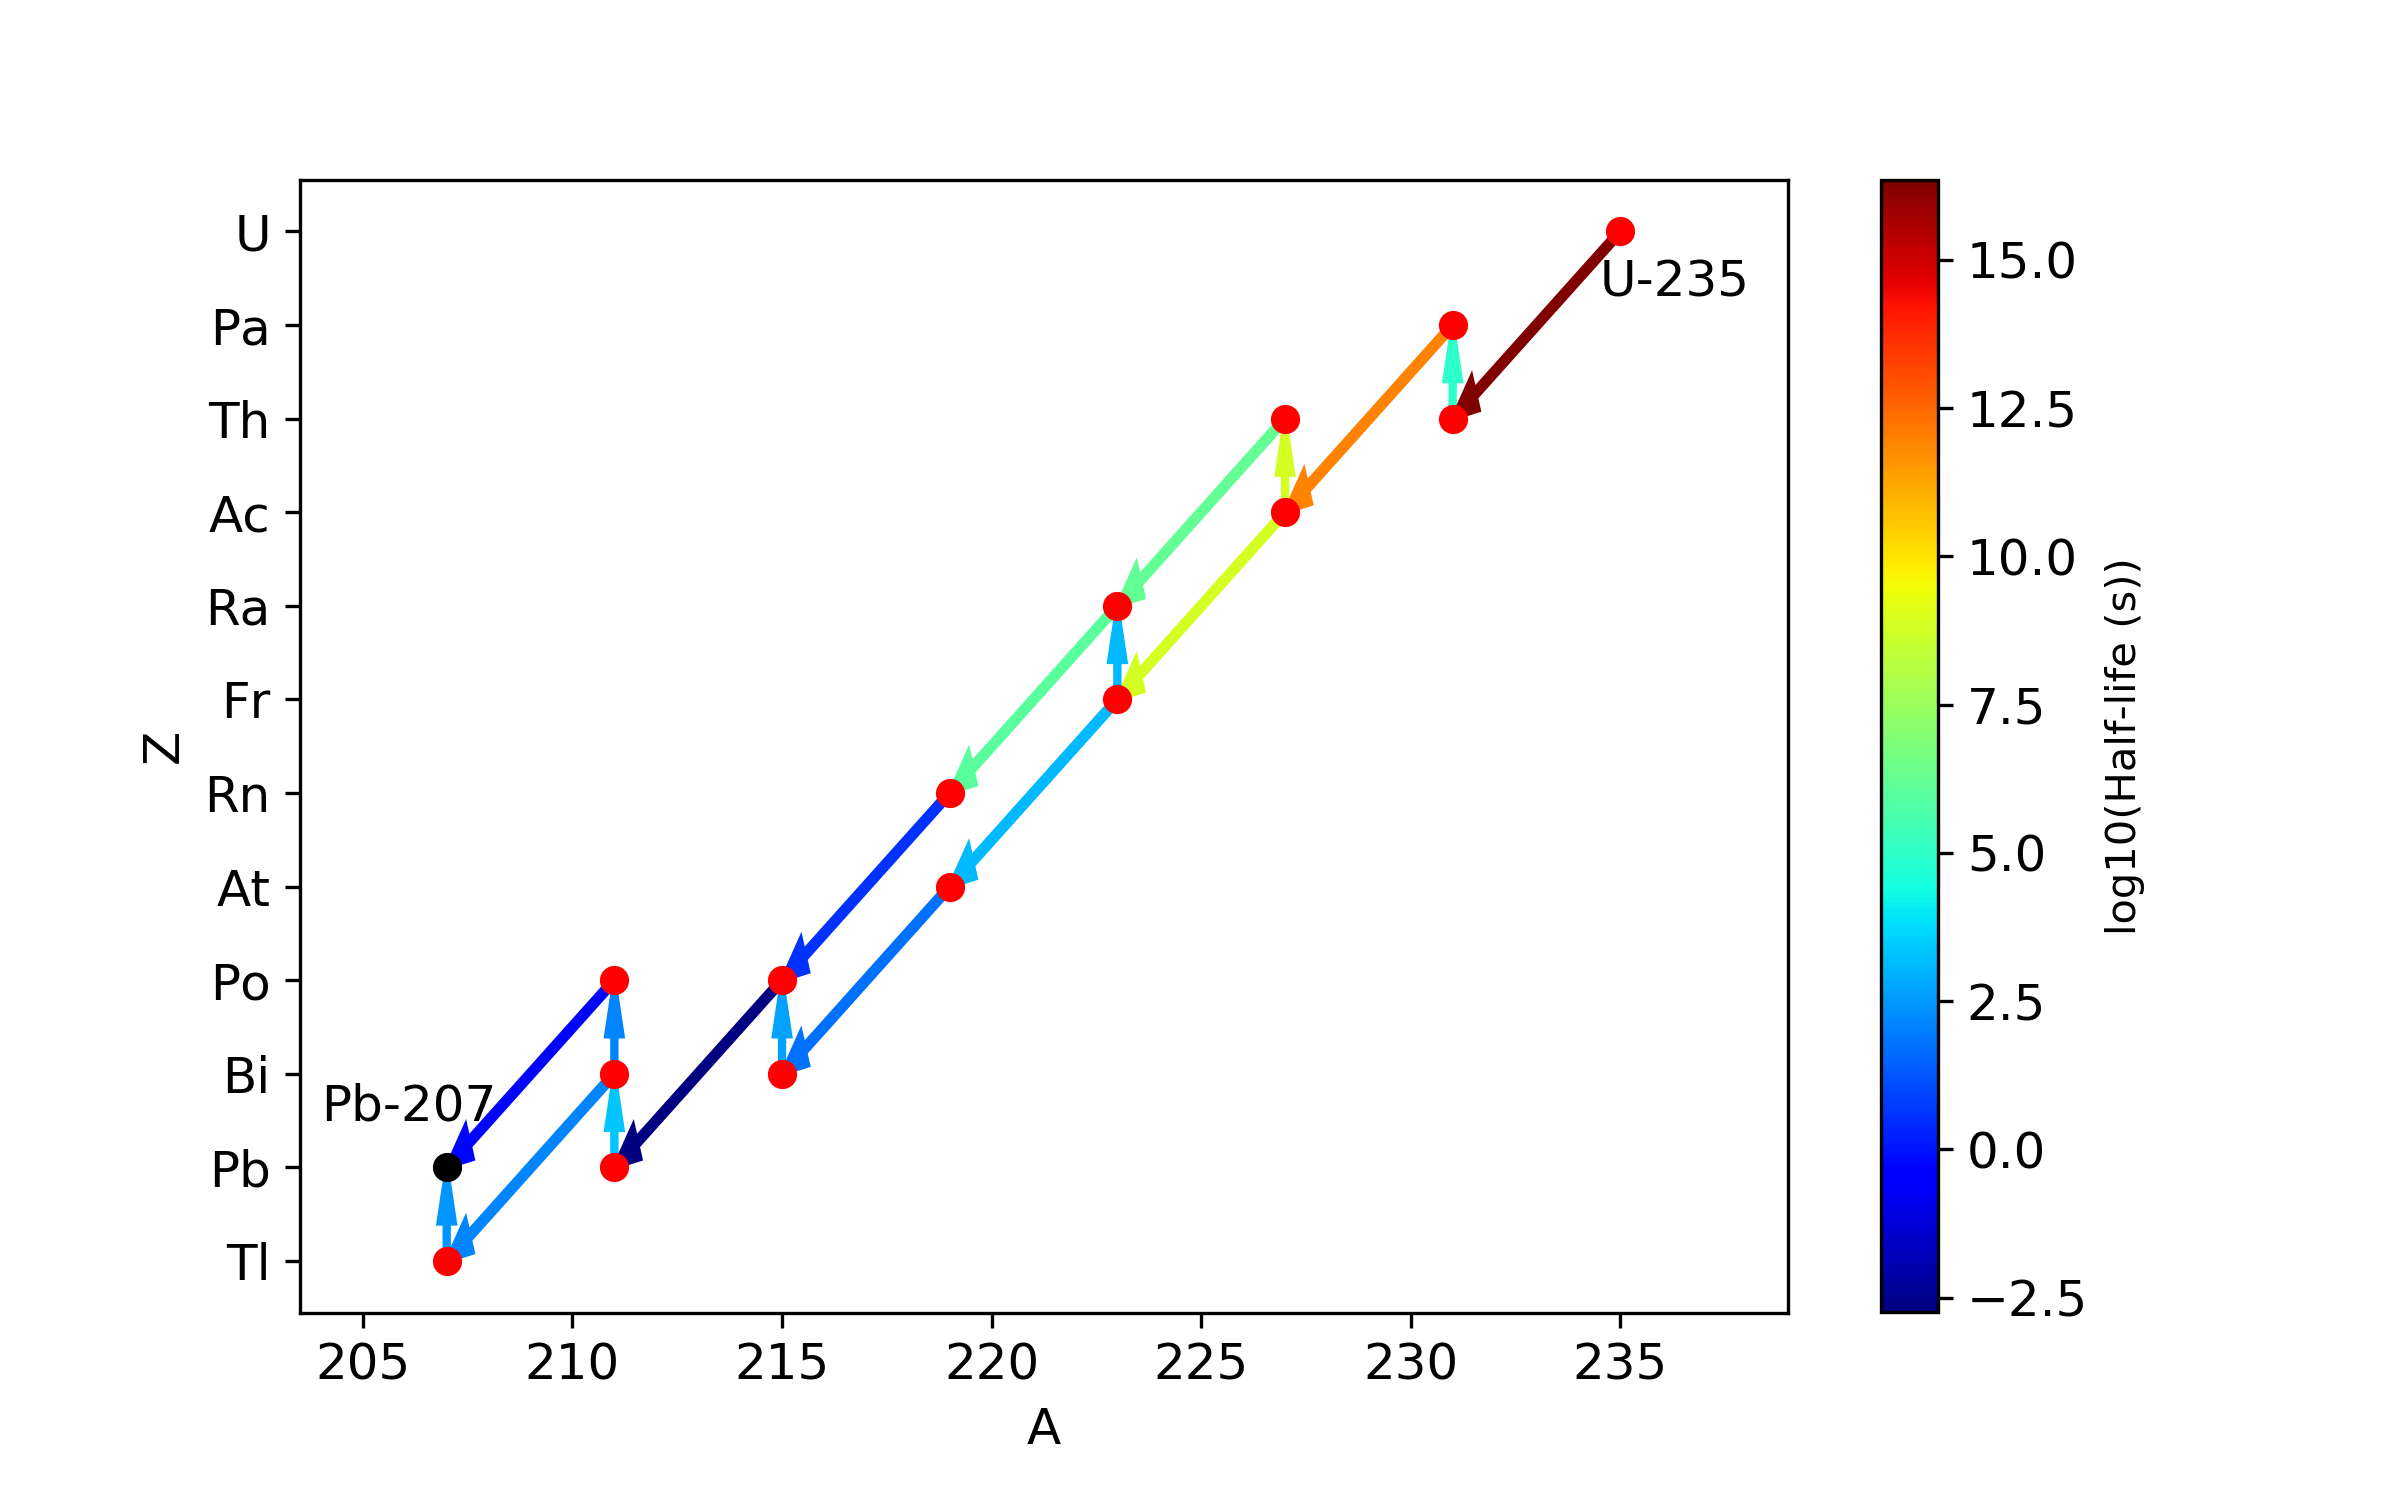
\includegraphics[scale=0.46] {figures/01-u235_decayseries.png}}\protect
\caption{\label{fig:decaychain} \footnotesize{${}^{235}U$ decay series.}}
\end{figure}

\subsubsection*{$\gamma$ decay}

As mentioned before $\gamma$ radiation is emitted during the transition between excited states. We can consider this reaction to be similar to a decay process, and characterize it with some decay constant $\lambda$. However, in this case due to quantum mechanical considerations we have to introduce the uncertainty or width $\Gamma$ of the energy level of the excited state. This width is related to the life time

\begin{equation}
\Delta E \Delta t \geq \hbar \rightarrow \Gamma=\hbar \lambda
\end{equation}

\subsection{Nuclear collision reactions}

When studying nuclear collision reactions between particles we can introduce similar notation as for chemical reactions:

\begin{equation}\label{eq:reaction}
a+X \rightarrow Y+b
\end{equation}

However in reactions relevant in reactor physics, one of the particles is often considered as a projectile and the other as a target (for example in the reactor the projectile, the neutron moves around in the system, whereas the target is often bound the a given location and changes locations only due to temperature induced fluctuations, for example U atoms in the fuel). In such reactions typically the outgoing particles can also be well distinguished in mass and type, however there are reactions (for example fission), where more particles appear after the reaction. A simple illustration of a nuclear collision reaction is given in Fig. \ref{fig:reactions}

\begin{figure}[ht!]
\protect \centering{

\includegraphics[scale=0.46] {figures/01-reactions.png}}\protect
\caption{\label{fig:reactions} \footnotesize{Illustration of nuclear collision events.}}
\end{figure}

Such reactions are often shorthanded as

\[
X(a,b)Y
\]

for example the neutron capture reaction on ${}_{92}^{235}U$ can be written as:

\[
{}_{92}^{235}U(n,\gamma){}_{92}^{236}U
\]

In general this class of reactions are often referred to as $(n,\gamma)$.

Since nuclear collision reactions are usually accompanied by the release or absorption of energy, it is often included in the notation. For the reaction \eqref{eq:reaction} one can calculate the reaction energy as

\begin{equation}\label{eq:reactionQ}
Q=[(m_a+M_X)-(M_Y+m_b)]c^2
\end{equation}

where Q is often referred to as the \textit{Q-value}. If $Q>0$, energy is released and the reaction is \textit{exothermic}. If $Q<0$, energy is required for the reaction to occur, the reaction is \textit{endothermic}.

As said before, there is a large variety of possible nuclear reactions, however the ones which are relevant for reactor physics involve the interaction of a neutron (as a projectile) and nuclei. These are

\begin{itemize}
\item Nuclear fission, $(n,fission)$
\item Radiative capture, $(n,\gamma)$
\item Elastic scattering, $(n,n)$ (the state of the target nucleus does not change)
\item Inelastic scattering, $(n,n')$ (the target nucleus becomes excited or a $\gamma$ photon is emitted promptly)
\item Several other reactions such as $(n,\textit{i}n)$, where $i$ number of neutrons are emitted from the target. $(n,p)$ and $(n,\alpha)$, where a proton or an $\alpha$ particle is emitted
\end{itemize}

As we will see later in light water reactors the fission, capture and elastic scattering reactions are dominating.

\subsection{Center of Mass vs LAB frame}

When we think about collision reactions, most naturally we imagine these in the laboratory or LAB frame, which means that the observer (for example we) is at a fixed point and always at rest. This is a rather intuitive frame, something we are used to since high school. However, the mathematical description of collision reactions it is often simpler in the center-of-mass or CM (sometimes CoM) frame, when the observer is at the center of mass of the system. 

\begin{figure}[ht!]
\protect \centering{

\includegraphics[scale=0.46] {figures/01-CoM.png}}\protect
\caption{\label{fig:LABCM} \footnotesize{LAB and CM frames.}}
\end{figure}

Let's consider the nucleus with mass $M$ at location $\mathbf{R}_L$ in the LAB frame and a neutron with mass $m$ at the location $\mathbf{r}_L$ in the LAB frame as illustrated in Fig. \ref{fig:LABCM}. We can then get the location of the center-of mass as 

\begin{equation}
\mathbf{\rho} = \frac{m\mathbf{r}_L+M\mathbf{R}_L}{m+M}
\end{equation}

from which we can convert the locations from LAB to CM as 

\begin{equation}
\mathbf{r}_C=\mathbf{r}_L - \mathbf{\rho}
\end{equation}

\noindent and

\begin{equation}
\mathbf{R}_C=\mathbf{R}_L - \mathbf{\rho}
\end{equation}

\noindent also

$$m\mathbf{r}_c + M\mathbf{R}_c = \mathbf{0}$$

We get similar formula for the velocities of the center of mass if we consider that the velocities in the LAB are $\mathbf{v}_L$ and $\mathbf{V}_L$ for the neutron and the nucleus. The center-of-mass travels with a velocity of

\begin{equation}
\mathbf{v}_{CM} = \frac{m\mathbf{v}_L+M\mathbf{V}_L}{m+M}
\end{equation}

And with that $\mathbf{v}_C=\mathbf{v}_L - \mathbf{v}_{CM}$ and $\mathbf{V}_C=\mathbf{V}_L - \mathbf{v}_{CM}$. Using such a reference frame is not always intuitive, however if we imagine that the target nucleus is at rest (which is usually not the case, since the target moves due to temperature, however this velocity is negligible for fast enough neutron energies), so $\mathbf{V}_L=0$, then the formalism further simplifies:

\begin{equation}
\mathbf{v}_{CM}=\frac{m}{m+M}\mathbf{v}_L
\end{equation}

\begin{equation}
\mathbf{v}_C=\mathbf{v}_L-\mathbf{v}_{CM}=\frac{M}{m+M}\mathbf{v}_L
\end{equation}

and

\begin{equation}
\mathbf{V}_C=-\mathbf{v}_{CM}=-\frac{m}{m+M}\mathbf{v}_L
\end{equation}

Thus the total momentum in CM is $\mathbf{p}_C=m\mathbf{v}_C+M\mathbf{V}_C=\mathbf{0}$, which means that the vector $\mathbf{v}_C$ and $\mathbf{V}_C$ are co-linear. In case of a scattering event, in the CM the particles are traveling towards each other before, and they travel back to back from each other after the scattering. Since in the following sometimes we will refer to the CM frame, it was important to introduce it at this stage. However, later we will use and review this formalism further to study the kinematics of elastic scattering reactions.

\subsection{Neutron cross sections}

The probability that a neutron interacts with a nucleus is characterized by the quantity called nuclear cross sections. The knowledge of this probability is essential to assess how a population of neutrons is going to be traveling in a nuclear reactor. 

\subsubsection{Microscopic cross sections}

Imagine a thin foil (one atomic layer thick, so no nuclei is shielded by any other) being bombarded by a beam of neutrons which have the same speed and which travel to the same direction. The rate of neutron-nuclear reactions will be proportional to the intensity $I$ of neutrons and to the number of atoms per unit area $N_A$, and the proportionality is given by $\sigma$

%\begin{figure}[ht!]
%\protect \centering{
%
\includegraphics[scale=0.46] {figures/placeholder.png}}\protect
%\caption{\label{fig:beam} \footnotesize{Illustration of collimated mono-energetic neutrons bombarding a thin foil.}}
%\end{figure}

\begin{equation}
R[\frac{\#}{cm^2s}]=\sigma [cm^2] I [\frac{\#}{cm^2s}] N_A [\frac{\#}{cm^2}]
\end{equation}

thus\footnote{Some might be bothered that $\#\#$ should be $\#^2$, but mathematically speaking we could substitute $\#=1$, and physically speaking we have to see that in $I$ the number $\#$ refers to neutrons, in $N_A$ it refers to nuclei, and in $R$ it refers to the reaction, which indeed needs both a neutron and a nucleus.}

\begin{equation}\label{eq:sigma}
\sigma=\frac{R}{IN_A}=\frac{R/N_A}{I}=\frac{\text{Number of reactions per nucleus per second}}{\text{Number of incident neutrons per cm}^2\text{ per second}}
\end{equation}

If we imagine the neutrons and the nuclei as classical particles (like solid spheres), then the proportionality constant $\sigma$ would be the cross sectional area of a single nucleus, therefore we call it \textit{microscopic cross section}. If we consider that the radius of a nucleus has a magnitude of $10^{-12}$ cm, then the cross sectional area would have a magnitude of $10^{-24}$ cm$^2$. Microscopic cross sections are measured in units of $10^{-24}$ cm$^2$, which we call $barn$ (often shorthanded as $b$).

Nevertheless, neutrons and nuclei do not behave as classical particles, thus one needs to take into account the quantum mechanical nature of such reactions, so the geometrical interpretation of the cross section is not always correct. Due to resonance effects, some nuclei will have very different microscopic cross sections very different from the geometrical cross sections. 

%It is also clear, that the probability per nuclear that a neutron interacts with it is $\sigma/A$, where A is the total cross sectional area.

\begin{figure}[ht!]
\protect \centering{

\includegraphics[scale=0.4] {figures/01-xshierarchy.png}}\protect
\caption{\label{fig:xshierarchy} \footnotesize{Hierarchy of reactions and cross sections.}}
\end{figure}

In a similar manner we could define microscopic cross sections for the various reaction types separately (eg. $\sigma_f$, $\sigma_e$ and $\sigma_c$ for fission, elastic scattering and capture respectively). Since this values are related to probabilities, we can sum them up, and define further cross sections, like the sum of elastic and inelastic scattering is the \textit{scattering cross section}

\[
\sigma_s=\sigma_e + \sigma_{in}
\]

or the sum of all cross sections is the \textit{total cross section}

\[
\sigma_t=\sigma_s + \sigma_{f}+ \sigma_{c} + ...
\]

which gives the probability that any reaction occurs. The absorption cross section can be define as 


\[
\sigma_a=\sigma_t - \sigma_s
\]

which gives the probability that a reaction resulting in the disappearance of the projectile neutron occurs. Note that some reactions will produce further neutrons, but as we will see when describing neutron transport usually we account for this by adding them separately. Fig. \ref{fig:xshierarchy} reviews the hierarchy of the cross sections. Note, that some textbooks consider (n,\textit{i}n) reactions as scattering reactions.

\subsubsection{Macroscopic cross sections}

In practical applications, such as in a nuclear reactor, the target is thicker than a foil (consider that a fuel pin is around a 1cm in diameter and is surrounded by few mm thick cladding and few cm of coolant and/or moderator material). In such situation most of the nuclei will be shielded by other nuclei, and the beam intensity changes inside the target. Let's look at an infinitesimally think layer between $[x,x+dx]$. The number of reactions in this layer is

\[
dR=\sigma_t I N dx
\]

\noindent where $N$ is the number density of nuclei. The change in the beam is therefore

\[
\frac{dI}{dx}=\frac{I(x+dx)-I(x)}{dx}=-\sigma_tI(x)N
\]

\noindent which, in case of $I(x=0)=I_0$ has the solution of

\[
I(x)=I_0\exp(-\sigma_tNx)
\]

Since the quantity $\sigma_t N$ appears often we prefer to introduce a new quantity, the \textit{macroscopic cross section}:

\[
\Sigma_t=\sigma_tN=[cm^{2}cm^{-3}=cm^{-1}]
\] 

\noindent which is related to the probability of interaction in a macroscopic sample (remember: the microscopic cross section was related to the probability of interaction per nucleus). However, this quantity is a cross section only in name. As we see it has inverse length units, and indeed it is rather related to the probability that an interaction happens over a certain distance traveled by the neutron. In fact

\begin{itemize}
\item $\exp(-\Sigma_t x)$ is the probability that a neutron travels a distance dx without participating in any interaction.
\item $\Sigma_t \exp(-\Sigma_t x)dx=p(x)dx$ is the probability that the neutron suffers an interaction in $[x,x+dx]$.
\end{itemize}

One can notice that $p(x)$ is a probability density function. Later we will learn how to sample such probability density function to sample random path lengths between collisions. For the moment we can however notice that it is possible to calculate the mean free path $\bar\lambda$ from

\[
\bar\lambda=\int\limits_0^\infty xp(x)dx=\frac{1}{\Sigma_t}
\]

Similarly we could define the collision frequency for neutrons traveling with speed $v$ as $v\Sigma_t$ and the mean time between interactions as $\frac{1}{v\Sigma_t}$.

The definition of macroscopic cross sections can be generalized to other reactions, for example fission ($\Sigma_f=N\sigma_f$), absorption ($\Sigma_a=N\sigma_a$) or scattering $\Sigma_s=N\sigma_s$, with which the total macroscopic cross section is

\[
\Sigma_t=\Sigma_a+\Sigma_s
\]

However the mean free path can be defined only for the total cross section (note that $\frac{1}{\Sigma_t} = \frac{1}{\sum\limits_i \Sigma_i}\neq \sum\limits_i\frac{1}{\Sigma_i}$)

One can also calculate the macroscopic cross section of homogeneous mixtures:

\[
\Sigma_t^{mix}=\sum\limits_i^M N_i\sigma_t^i \quad \text{for i=1,2,...M nuclides}
\]

\begin{tcolorbox}
\textbf{Exercise}

Consider a control rod made of boron carbide ($\text{B}_4\text{C}$) with natural boron. Natural boron consists of two stable isotopes: B-11 (80.1\%) and B-10 (19.9\%). Determine the total macroscopic cross-section and the mean free path of a neutron in boron carbide if
\begin{itemize}
\item $\rho = 2.52\text{g}/\text{cm}^3$
\item $M_B = 10.8\text{g}/\text{mol}$
\item $M_C = 12\text{g}/\text{mol}$
\item $\sigma_{\text{B-10}}=3843 \text{b}$, $\sigma_{\text{B-11}}=5.07 \text{b}$, $\sigma_{\text{C-12}}=5.01 \text{b}$

$$\Sigma=\frac{\rho N_A}{M_{B_4C}}\sum_in_i\sigma_i$$
$$\Sigma=\frac{\rho N_A}{4M_{B}+M_{C}}(4\sigma_B+\sigma_C)$$
$$\Sigma=\frac{\rho N_A}{4M_{B}+M_{C}}(4(0.801\sigma_{B-11}+0.199\sigma_{B-10})+\sigma_C)=84.4 \: \text{cm}$$
$$\lambda=\frac{1}{\Sigma}=0.11\:\text{mm}$$
\end{itemize}
 \end{tcolorbox}

As we will see shortly, the microscopic cross section has strong dependence on the neutron energy, therefore the macroscopic cross section also has the same dependence. However, the number density can have strong variations in space and in time as well (for example reactors are heterogeneous systems, so the material composition varies between various locations, and as we will see later, over time due to depletion the composition does change), therefore the macroscopic cross sections often also have strong dependence on these variables:

\[
\Sigma (E, r, t)=N(r,t)\sigma (E)
\]

\subsubsection{Reaction rate and flux}

As stated above, the collision frequency for neutrons traveling with speed $v$ is 

\begin{equation}
\text{collision frequency}=v\Sigma_t
\end{equation}

\noindent Now, let's define the neutron population as 

\begin{equation}
n(t)=\text{Number of neutrons per unit volume }(1/\text{cm}^3)
\end{equation}

\noindent then the number of reactions over time and over unit volume would be

\begin{equation}
R(t)=\text{Reaction rate density}=n(t)v\Sigma_t \quad (1/(\text{cm}^3s))
\end{equation}

\noindent where the quantity $vn(t)$ appears so often in reactor physics that it is used to describe the neutron population and is called neutron flux

\begin{equation}
\phi(t)=\text{Neutron flux}=vn(t) \quad (1/(\text{cm}^2s))
\end{equation}

As we will see later, the neutron flux and the neutron density can be introduced in a more general manner when they depend on the location, neutron energy, and even the direction the neutrons travel towards. Although the main reason for using the neutron flux to describe the neutron population is because it is a convenient variable, it does have a physical meaning: the total distance traveled in a volume per second by neutrons. Note that often the reaction rate $R$ is related to the reaction rate in $1/s$ units, some textbooks therefore highlight density like quantities as $R'''$, we will not follow this notation, and use $R$ regardless it is reaction rate or reaction rate density, nevertheless we will try to be transparent in the text.


\subsubsection{Characteristics of microscopic cross sections}

Previously we have assumed that the beam contains mono-energetic neutrons traveling to the same direction. This however is not the case in a nuclear reactor. Furthermore, the microscopic cross sections do depend strongly on the energy, and rather weakly on the direction of the neutrons. It is therefore important to review the characteristics of cross sections. Here we focus on the fundamental physical mechanism involved in collision events, and later we will also review the kinematics of collision.

There are two main mechanism interesting for reactor physics:

\begin{itemize}
\item Potential scattering: when a neutron does not penetrate the nucleus, only scatters off its force field.
\item Compound nucleus formation: when the neutron penetrates the nucleus, and a new nucleus with $A+1$ is created, which then disintegrates either by emitting gamma photons, neutrons or undergoes fission.
\end{itemize}

Potential scattering can be handled in classical terms, as we will see later. The magnitude of the cross section for this reaction is essentially the geometrical cross section of the nucleus, and the energy dependence is flat over a wide range of energies as shown in Fig. \ref{fig:h1scatter}. Later we will investigate the kinematics of these events further to understand how neutrons loose their energy in scattering events.

\begin{figure}[ht!]
\protect \centering{
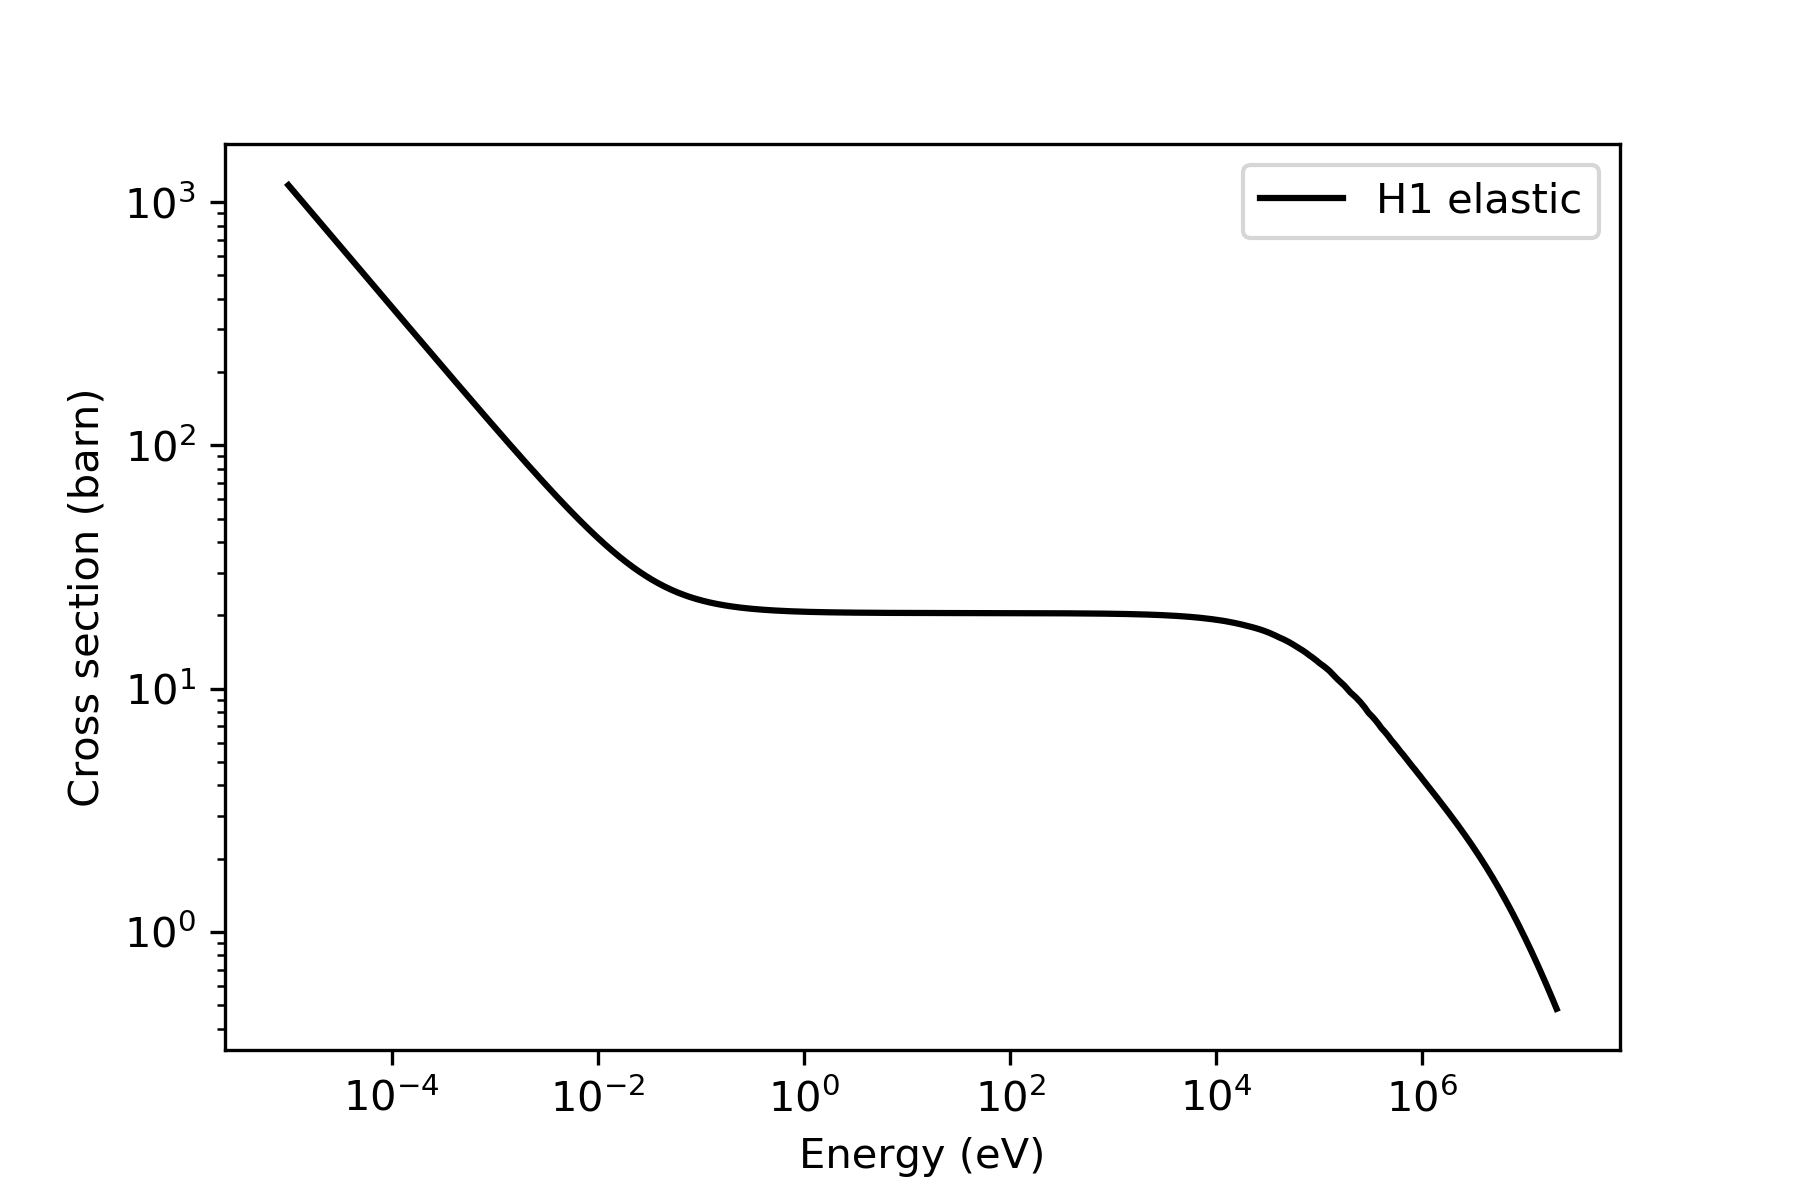
\includegraphics[scale=0.46] {figures/01-H1scattering.png}}\protect
\caption{\label{fig:h1scatter} \footnotesize{Elastic scattering cross section on Hydrogen-1.}}
\end{figure}

In compound nucleus formation however a new nucleus is formed. The time scale of this event is cca. 1000 times longer than it would take for the neutron to go through the nucleus. This tells us both that indeed something is happening there, and also this time is enough for the outcoming particles to "forget" what happened with them before (for example the the direction of the incoming neutron). Compound nucleus formation happens in many reactions: in fission, radiative capture and scattering:

\begin{equation}
    {}_Z^AX + n \rightarrow {}_Z^{A+1}X^*
    \begin{cases}
      a: \text{elastic scattering} \\
      b: \text{inelastic scattering} \\
      c: \text{radiative capture} \\
      d: \text{fission}
    \end{cases}
\end{equation}
    
In compound nucleus formation if the CM energy of the neutron plus the binding energy ($[M(A+1,Z)-M(A,Z)-m_n]c^2$) of the neutron matches an energy level of the compound nucleus then the magnitude of the cross section increases (often with several orders of magnitude). This is shown in Fig. \ref{fig:nalevels} for the capture cross section of Na-23. Then we refer to the "resonance" of Na-23, eventhough fundamentally the resonance corresponds to the energy level of the compound Na-24 nucleus. Resonances have different width, which depends on the lifetime of the energy level.

\begin{figure}[ht!]
\protect \centering{
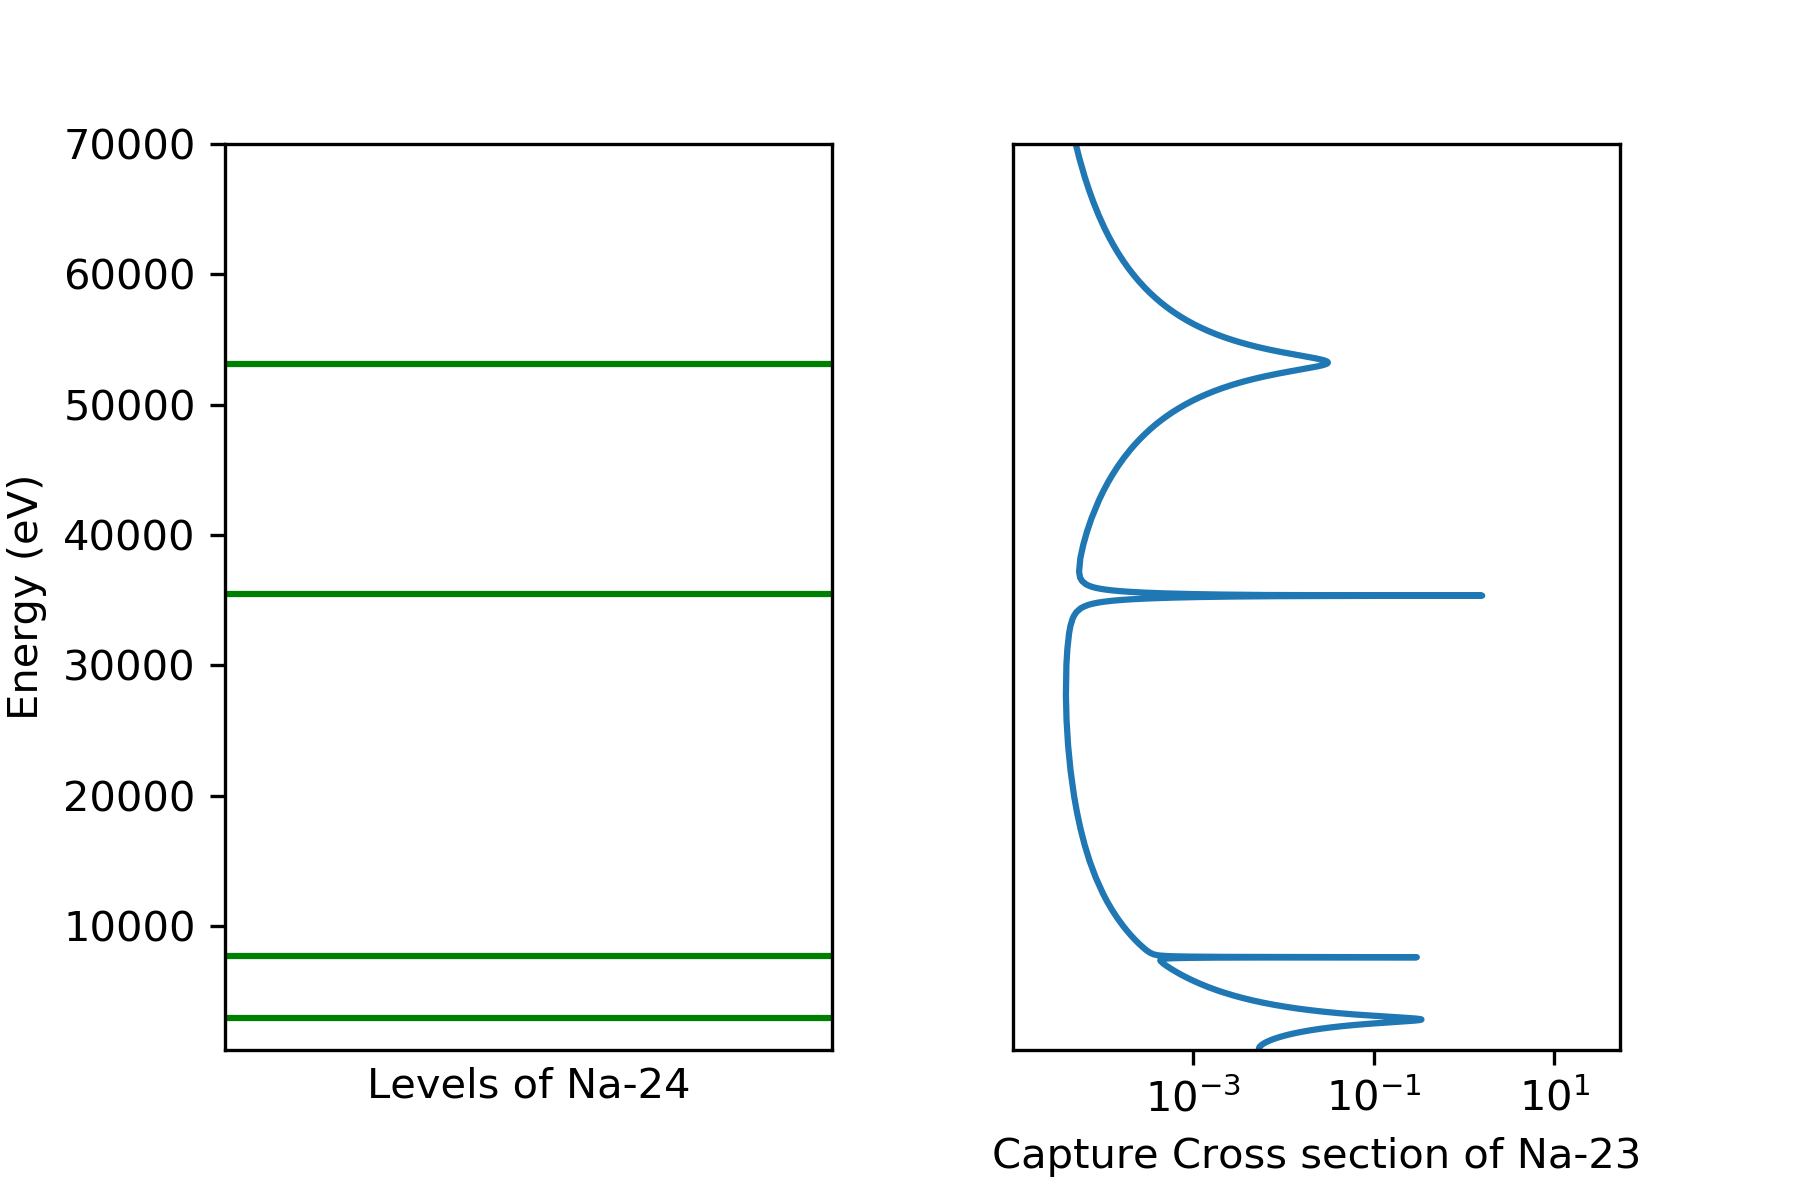
\includegraphics[scale=0.46] {figures/01-na23xs-levels.png}}\protect
\caption{\label{fig:nalevels} \footnotesize{The levels of Na-24 and the capture cross section of Na-23.}}
\end{figure}

Although the cross section of various reactions show similarities due to the shared underlying physics, the outcome and some characteristics are different, so we will review them one by one. All the reactions are summarized in Fig. \ref{fig:levels}.

Notice that the compound nucleus will have energy levels below the ground state of the target nucleus. These levels cannot be directly reached from neutron reactions, and are sometimes referred to as "negative resonances". They have some impact on the cross sections, but the discussion of this impact is well outside of the subject of this text book.

\begin{figure}[ht!]
\protect \centering{
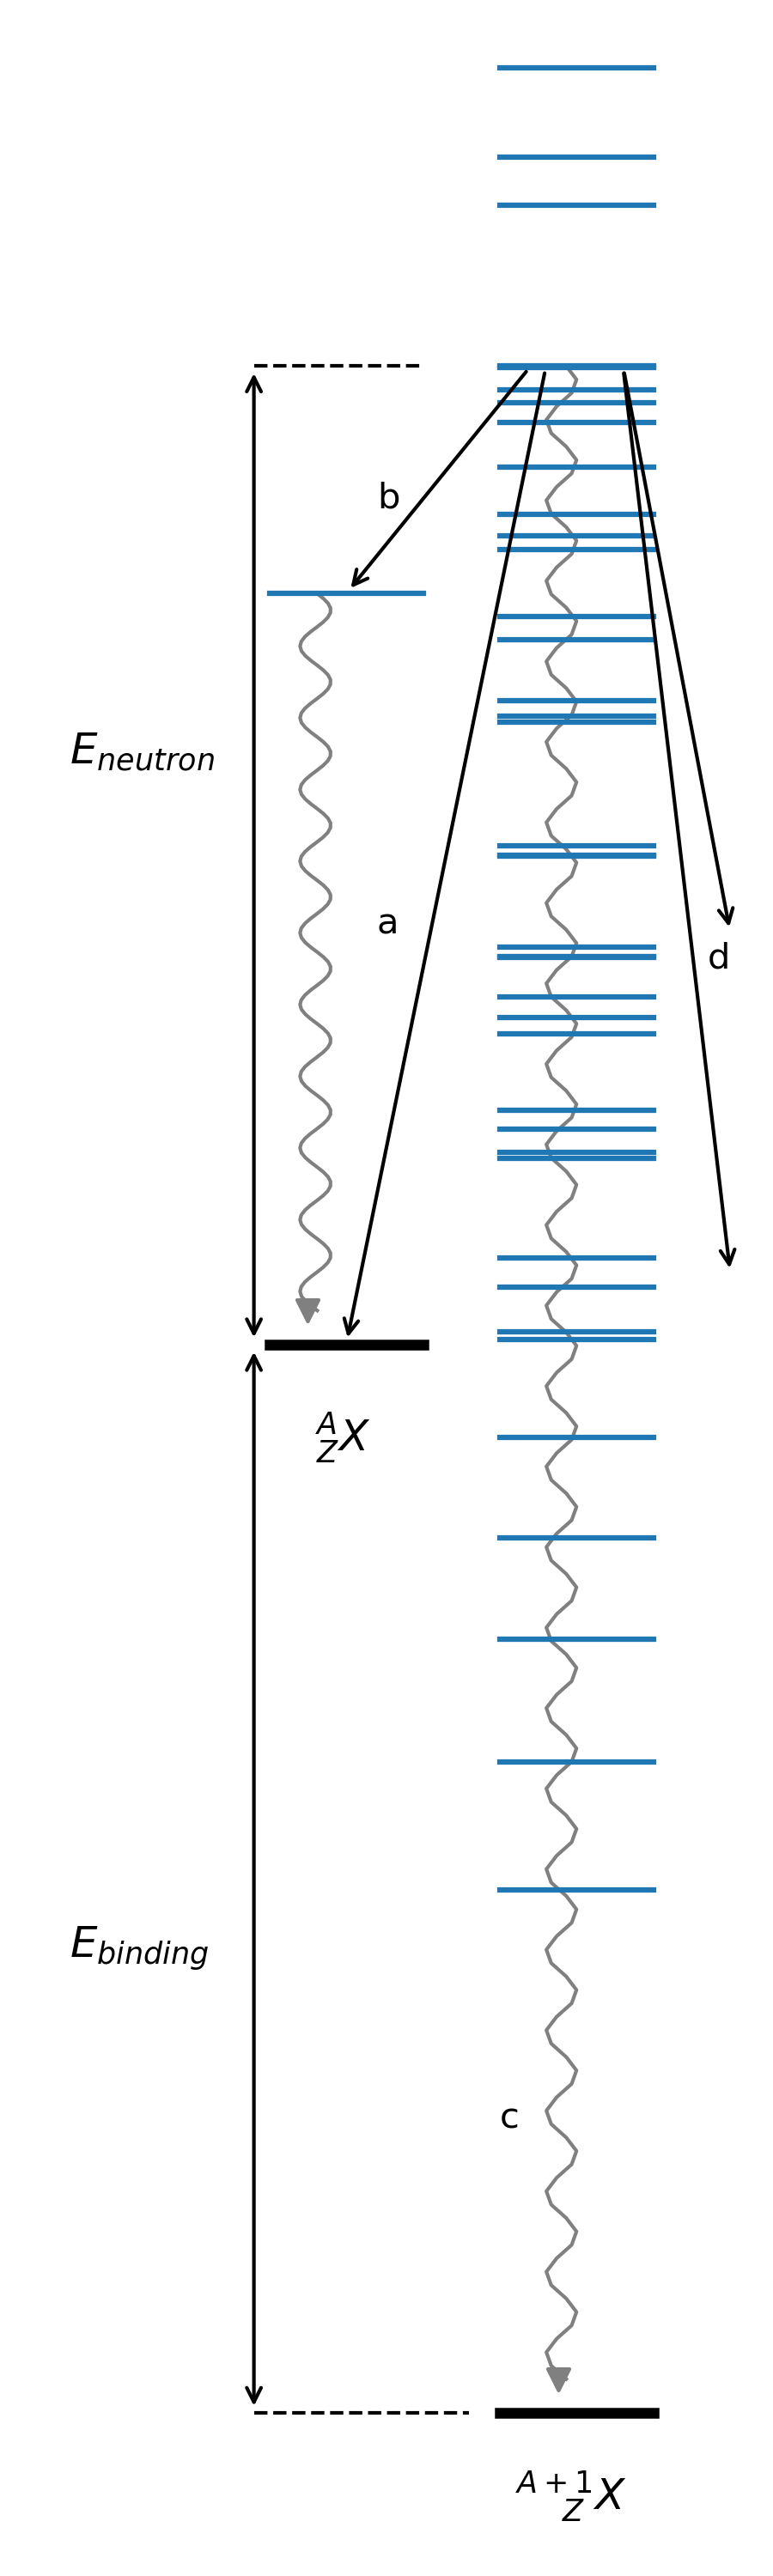
\includegraphics[scale=0.66] {figures/01-reactionlevels.png}}\protect
\caption{\label{fig:levels} \footnotesize{Schematic illustration of various reactions after compound nucleus formation. (a: elastic scattering, b: inelastic scattering, c: radiative capture, d: fission)}}
\end{figure}


\subsubsection*{Radiative capture}

In radiative capture when the CM energy of the neutron and the binding energy matches an energy level of the compound nucleus will be created in an excited state. The compound nucleus emits a cascade of $\gamma$-photons to reach the ground state (note that in Fig. \ref{fig:levels} only one $\gamma$ is highlighted with a curly line, but in fact several photons can be emitted).

At low energies the energy levels of the compound nucleus are far from each other, however for higher energies, and especially for heavy nuclides, the energy levels become very dense, and it is not possible with current measurements to resolve them. This region we call unresolved resonance region (URR), which usually gives a lot of headache to nuclear reactor physicist, however at this level we will not need to worry about this. Fig. \ref{fig:u238cap} shows the capture cross section of U-238. We can observe that at lower neutron energies (below 100 eV) the single resonances can be seen, but for higher energies the resonances overlap. At even higher energies it seems that the cross section becomes suddenly smooth. At these energies the resonances are so tightly packed that they cannot be resolved experimentally at all.


\begin{figure}[ht!]
\protect \centering{
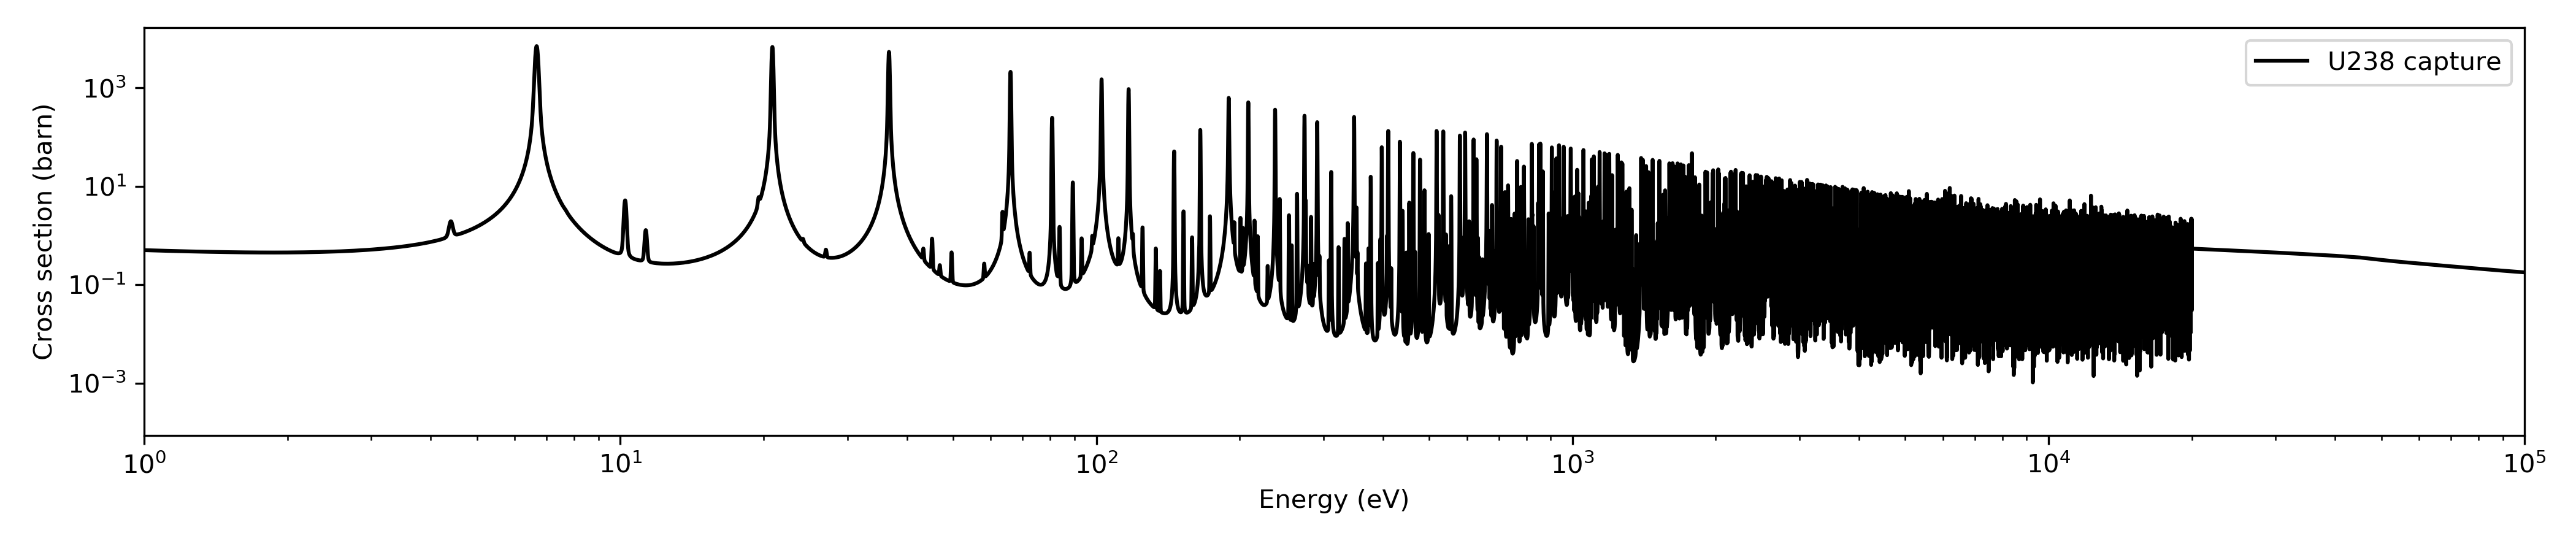
\includegraphics[scale=0.46] {figures/01-u238-capture.png}}\protect
\caption{\label{fig:u238cap} \footnotesize{Radiative capture cross section of U-238.}}
\end{figure}

One can use the Single-level Breit-Wigner (SLBW) model to describe such resonances, which will also predict that at low energies the cross section will have a $1/E^{1/2}$ or $1/v$ behavior. You can find further details on the SLBW model in the course books. This behavior can be understood phenomenologically: the slower the neutron is, the more time it spends around the nucleus, thus the higher the probability of entering a reaction. 

\subsubsection*{Fission}

In fission the excited compound state relaxes down by emitting several (most often 2-3) neutrons, and the compound nucleus splits into two (or seldom three) nuclei. 

The cross section is similar to that of the radiative capture reaction. However, as shown in Fig. \ref{fig:ufission}, some nuclides have a threshold for fission at high energies. This is due to the various size of the fission barrier. If a nuclide does not have such a threshold, and tends to undergo fission at low neutron energies as well, we call it \textit{fissile}, and nuclides which undergo fission only due to interaction with high energy (or fast) neutrons are called \textit{fissionable}.

\begin{figure}[ht!]
\protect \centering{
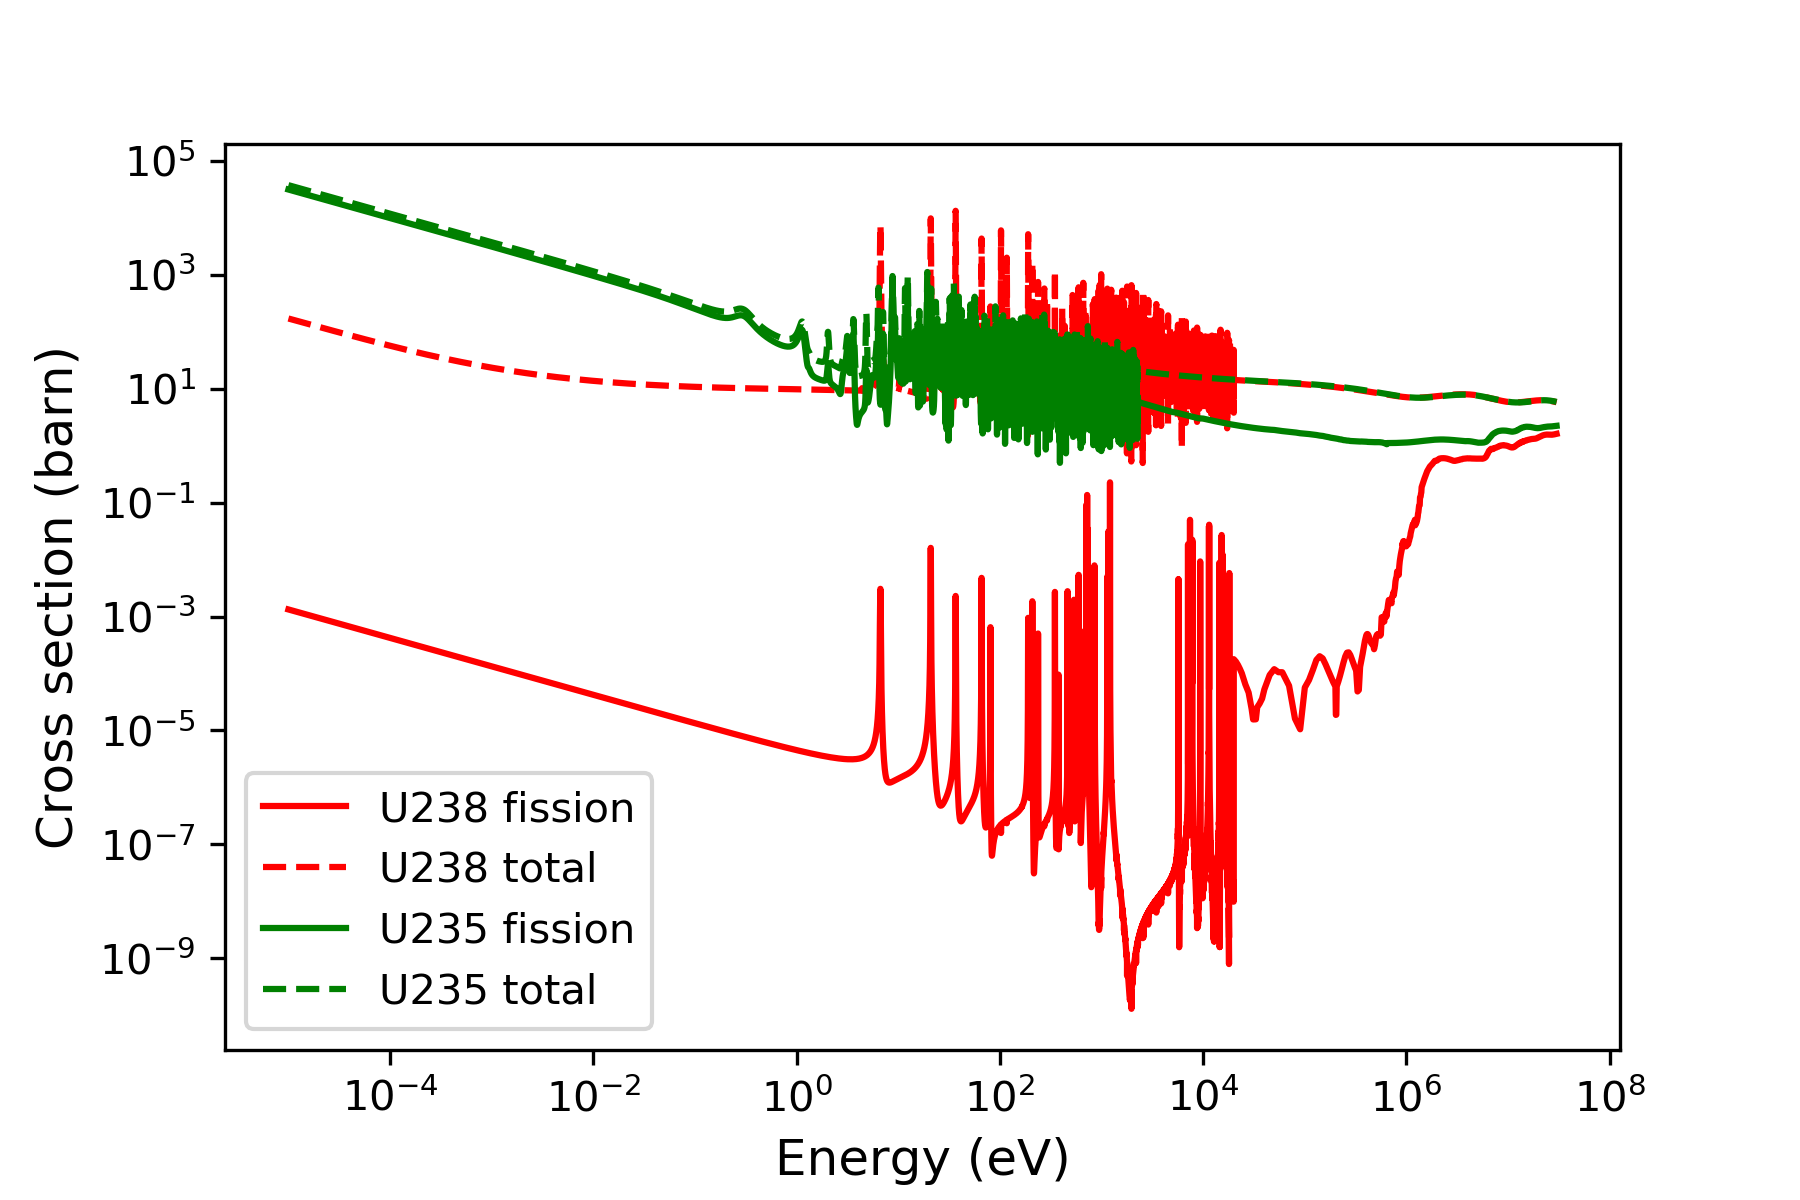
\includegraphics[scale=0.56] {figures/01-Ufission.png}}\protect
\caption{\label{fig:ufission} \footnotesize{Fission and total cross section of U-238 and U-235.}}
\end{figure}

\subsubsection*{Inelastic scattering}

In inelastic scattering the ingoing neutron is reemitted, but after the neutron emission the target nucleus is in an excited state, therefore $\gamma$-photons are emitted to reach the ground state of the target nucleus. In such a reaction the neutron can loose a lot of energy, and the kinetic energy is not conserved. However for inelastic scattering to happen the ingoing neutron needs to have more kinetic energy than the first energy level of the target nucleus. This is shown for C-12 in Fig. \ref{fig:c12inelastic}. The threshold energy is usually several MeV, thus in typical light water reactors this reaction has little role. However for fast reactors it is often necessary to consider such reactions.

\begin{figure}[ht!]
\protect \centering{
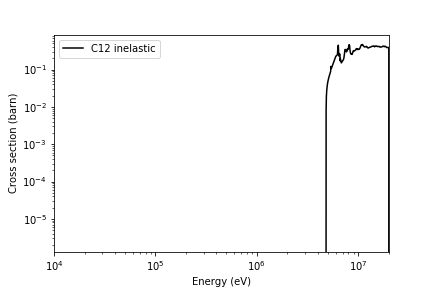
\includegraphics[scale=0.46] {figures/01-c12inelastic.png}}\protect
\caption{\label{fig:c12inelastic} \footnotesize{Inelastic scattering cross section of C-12.}}
\end{figure}

\subsubsection*{Elastic scattering}

Elastic resonance scattering happens when the compound nucleus emits a neutron, and as a result the target nucleus returns to its ground state. In this reaction the kinetic energy of the neutron is conserved. Nevertheless the cross section of such reactions is somewhat different as for the other reactions. The reason for this is that the elastic scattering cross section has three components: the previously discussed \textit{potential scattering}, the resonance scattering, and the interference scattering component. The last one is a quantum mechanical effect, and as a result the cross section may decrease before the resonance. This is shown in Fig. \ref{fig:u238elastic}.

\begin{figure}[ht!]
\protect \centering{
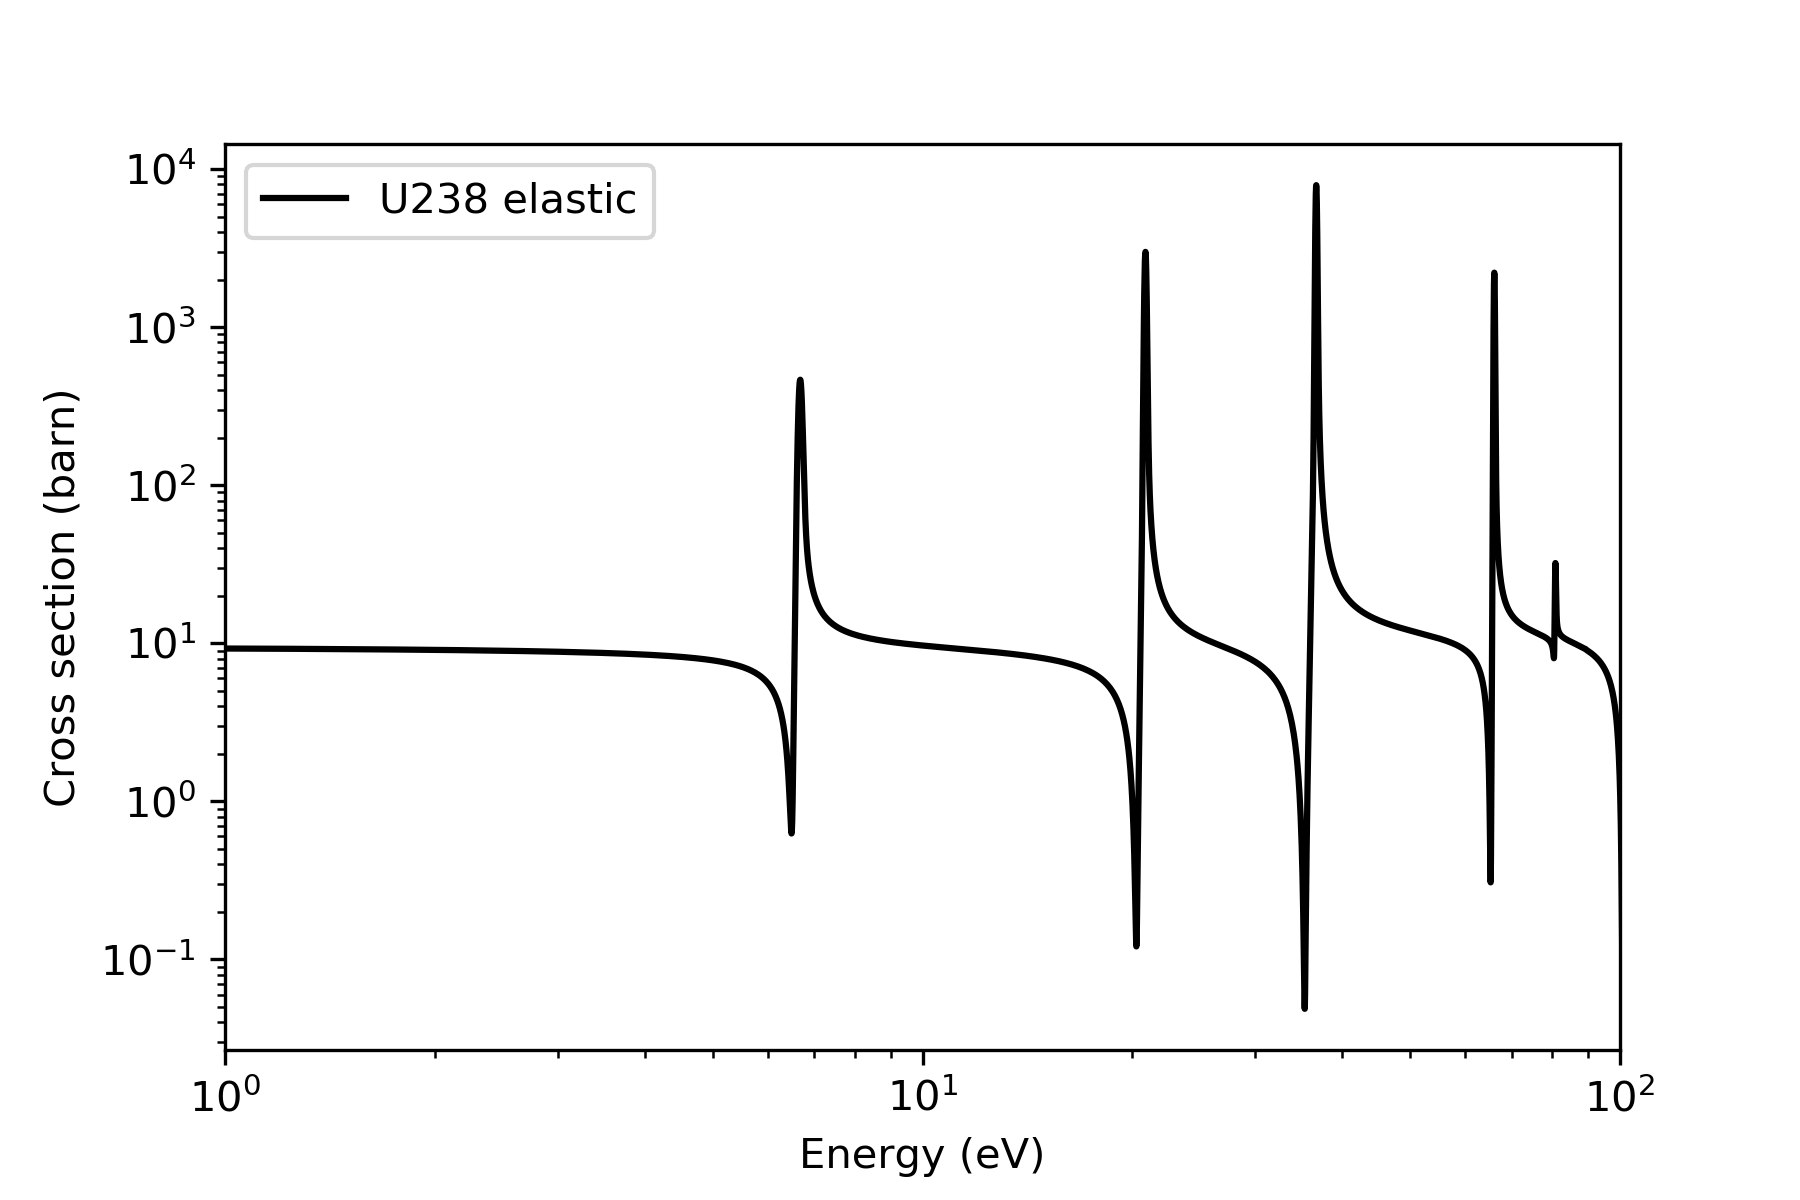
\includegraphics[scale=0.46] {figures/01-u238-resonancescatter.png}}\protect
\caption{\label{fig:u238elastic} \footnotesize{Resonances in the elastic scattering cross section of U-238.}}
\end{figure}

\subsubsection{Nuclear data libraries}

It is by now obvious that decent reactor analysis can only be done if good nuclear data is available. The various cross sections of several nuclides are measured by several laboratories, and the data is published. The standard format is called ENDF (evaluated nuclear data file), and all institutes publish the data as ENDF files. These cross sections are so called point wise cross sections: cross section evaluations at certain energies. Then the user can interpolate between the energies to obtain the cross section at any arbitrary energy. As we will see later, most of the reactor physics methods require data weighted by some function describing the energy distribution of neutrons and integrated over energy groups. This is the task of nuclear data processing tools (the most widespread code is called NJOY). Such codes can also convert the ENDF files into other formats which are then used by neutron transport codes.

There are several evaluations, which do have slight differences due to the obvious limitation of measurements. Researchers perform uncertainty studies often by executing the same calculation with various nuclear datasets. Some of the important libraries are ENDF/B-VIII.0 (from the US), JEFF-3.3 (the Joint Evaluated Fission and Fusion File). 

You can access raw ENDF files from various sources, for example the Nuclear Data Services of IAEA (\url{https://www-nds.iaea.org/} or from the Nuclear Data Center of KAERI (\url{http://atom.kaeri.re.kr/}).

Since in a recorded video lecture we will review how to access and plot these files, we will not go into further detail in this lecture note. 

\subsection{Generalization of the scattering cross section}

For scattering reactions both the energy and the direction of the particle might change. Nevertheless the value $\sigma_s(E)$ only quantifies the probability that a scattering event at neutron energy $E$ takes place. We might be however interested in the probability that the scattering results in a certain outgoing energy and direction. To describe this we can introduce differential cross sections:
\begin{itemize}
\item $\sigma_s(E\rightarrow E')$ quantifies the probability that a scattering event changes the ingoing neutron energy $E$ to $E'$ in $dE'$. Thus this cross section is in fact a distribution with unit cm$^2/$eV, and often noted with $d\sigma/dE$
\item $\sigma_s(\mathbf{\Omega}\rightarrow \mathbf{\Omega}')$ quantifies the probability that a scattering event changes the initial neutron direction $\mathbf{\Omega}$ to $\mathbf{\Omega}'$. It is often noted with $d\sigma/d\Omega$.
\end{itemize}

The name "differential cross section" is even more obvious when we consider that

$$\sigma_s(E)=\int\limits_0^\infty\sigma_s(E\rightarrow E')dE'$$

$$\sigma_s(\mathbf{\Omega})=\int\limits_{4\pi}\sigma_s(\mathbf{\Omega}\rightarrow \mathbf{\Omega}')d\mathbf{\Omega}'$$

It is however important to highlight that the dependence of $\sigma_s(\mathbf{\Omega})$ on the direction is weak, because in reactor applications the nuclei are randomly orientated within the materials. Similarly, $\sigma_s(\mathbf{\Omega}\rightarrow\mathbf{\Omega}')$ will usually not depend on the incident neutron direction, it is rather the change in the direction which is of importance, which change can be given by the cosine of the scattering angle $\theta$, which is in fact the dot product of the before and after directions $\mu_0=\mathbf{\Omega}\mathbf{\Omega}'$, therefore often one just simply uses the notation

$$\sigma_s(\mathbf{\Omega}\rightarrow \mathbf{\Omega}')=\sigma_s(\mathbf{\Omega}\mathbf{\Omega}')=\sigma_s(\mu_0)$$

By combining the differential cross sections one can define the double differential scattering cross section

$$\frac{d\sigma_s^2}{dEd\mathbf{\Omega}}=\sigma_s(E\rightarrow E',\mathbf{\Omega}\rightarrow \mathbf{\Omega}')$$

\noindent from which

$$\sigma_s(E\rightarrow E')=\int\limits_{4\pi}\sigma_s(E\rightarrow E',\mathbf{\Omega}\rightarrow \mathbf{\Omega}')d\mathbf{\Omega}'$$

$$\sigma_s(E,\mathbf{\Omega}\rightarrow \mathbf{\Omega}')=\int\limits_{0}^\infty\sigma_s(E\rightarrow E',\mathbf{\Omega}\rightarrow \mathbf{\Omega}')dE'$$

$$\sigma_s(E)=\int\limits_{4\pi}\int\limits_{0}^\infty\sigma_s(E\rightarrow E',\mathbf{\Omega}\rightarrow \mathbf{\Omega}')dE'd\mathbf{\Omega}'$$

\noindent and these concept can be generalized to the macroscopic cross sections. Analyzing and handling such data is not straightforward. However, there is one situation when the handling is not difficult: elastic potential scattering in case of isotropic scattering angle in the CM system. Some books (such as Stacey: Nuclear reactor physics) quote the relationship $\mu_c=0.07A^{2/3}E(MeV)$, which indeed is close to zero below cca 0.1 MeV for light nuclei), others (such as D\&H) quote that this is applicable for neutron energies below 1MeV for light nuclei. In this case the scattering kernel is separated as

$$\sigma_s(E\rightarrow E')=\sigma_s(E)P(E\rightarrow E')$$

\noindent where $P(E\rightarrow E')dE'$ is the probability that a neutron with initial energy $E$ will have an energy $E' \in [E',E'+dE']$. Probability density functions like these are often referred to as \textit{scattering kernels}. In the following we will investigate this probability density function for elastic scattering.

\subsection{Scattering kernel and kinematics}

As mentioned earlier, studying the kinematics of elastic neutron scattering is simpler in the center-of-mass system. The reason is that in the laboratory system the target nucleus recoils after the scattering event (due to momentum is conserved), thus the energy of the neutron get smaller with the same amount of energy what is acquired by the recoiling nucleus. However in the CoM the energies of the neutron and the nucleus are the same, and only the direction changes. 

We have earlier introduced the Center-of-Mass and Laboratory frames. Let us now further elaborate, and study the situation when a neutron elastically scatters on a target nucleus at rest (in the laboratory). Figure \ref{fig:cmlabscatter}. In the CM system, the center-of-mass is fixed, thus the target nucleus travels towards the collision. After collision the speed of the nucleus and the neutron is not changed, only the direction, the nucleus and the target travel back to back. Figure \ref{fig:cmlabrelation} shows how the two systems and the scattering angles are related to each other.

\begin{figure}[ht!]
\protect \centering{

\includegraphics[scale=0.46] {figures/01-CM-LAB_scatter.png}}\protect
\caption{\label{fig:cmlabscatter} \footnotesize{Scattering in the laboratory and center-of-mass.}}
\end{figure}

\begin{figure}[ht!]
\protect \centering{

\includegraphics[scale=0.46] {figures/01-CM-LAB_relation.png}}\protect
\caption{\label{fig:cmlabrelation} \footnotesize{Relation of the laboratory and center-of-mass.}}
\end{figure}

After considering momentum and energy conservation and some elementary geometry, we can arrive to following important formula (for full derivation see D\&H p40) relating the kinetic energy in the LAB before and after the collision.

$$\frac{E'}{E}=\frac{A^2+2A\cos\theta_C+1}{(A+1)^2}$$

\noindent and by introducing 

$$\alpha=\Big(\frac{A-1}{A+1}\Big)^2$$

\noindent we can rearrange to

\begin{equation}\label{eq:muErelation}
\frac{E'}{E}=\frac{(1+\alpha)+(1-\alpha)\cos\theta_C}{2}
\end{equation}

\noindent which shows that the energy transfer from the neutron to the nucleus is directly related to the scattering angle in CM. The $\theta_C=180^\circ$ heads on collision results in a backscattered neutron with an energy $\alpha E$, thus the maximum energy the neutron can loose is $(1-\alpha)E$. In case of a hydrogen target nucleus ($\alpha=0$), the neutron can loose all its energy. However for a uranium-235 scatterer the neutron can loose only 1.7\% of its energy.

We can also see that the neutron energy after the scattering is always less than before. This however is a consequence of our assumption that the target is at rest.

Since we discovered that the scattering angle is directly related to the energy transfer, we can also presume that the probability distribution $P(E\rightarrow E')$ is directly related to the probability of scattering with an angle $\theta_C \in [\theta_C,\theta_C+d\theta_C]$. Let us use the cosine of the scattering angle $\mu_C=\cos\theta_C$ and consider that its distribution is given with $\chi(\mu_C)$. We see from Eq. \eqref{eq:muErelation} that a given $d\mu_C$ corresponds to a given $dE'$, thus 

$$P(E\rightarrow E')dE'=\chi(\mu_C)d\mu_C$$

\noindent and from  Eq. \eqref{eq:muErelation} we see that

$$d\mu_C=\frac{2dE'}{(1-\alpha)E}$$

\noindent therefore

\begin{equation}
    P(E\rightarrow E') = 
    \begin{cases}
      \frac{2\chi(\mu_C)}{(1-\alpha)E} & \text{if} \: \alpha E \leq E' \leq E \\
      0 & \text{otherwise}
    \end{cases}
\end{equation}

However, as we said before, we can safely assume below 100 keV that scattering is isotropic in the CM frame. In that case, the cosine $\mu_C$ is uniformly distributed between $[-1,1]$, therefore

$$\chi(\mu_C)=\frac{1}{2}$$

\noindent and with that the scattering kernel is

\begin{equation}
    P(E\rightarrow E') = 
    \begin{cases}
      \frac{1}{(1-\alpha)E} & \text{if} \: \alpha E \leq E' \leq E \\
      0 & \text{otherwise}
    \end{cases}
\end{equation}

\noindent which means that the outgoing energy is also uniformly distributed between $[\alpha E, E]$ as shown in Figure \ref{fig:isotroppdf}. With this the differential scattering cross section of elastic scattering becomes.

\begin{equation}
    \sigma_s(E\rightarrow E') = 
    \begin{cases}
      \frac{\sigma_s(E)}{(1-\alpha)E} & \text{if} \: \alpha E \leq E' \leq E \\
      0 & \text{otherwise}
    \end{cases}
\end{equation}

\noindent and as we saw before the potential scattering cross section is only weakly dependent on the energy.

\begin{figure}[ht!]
\protect \centering{
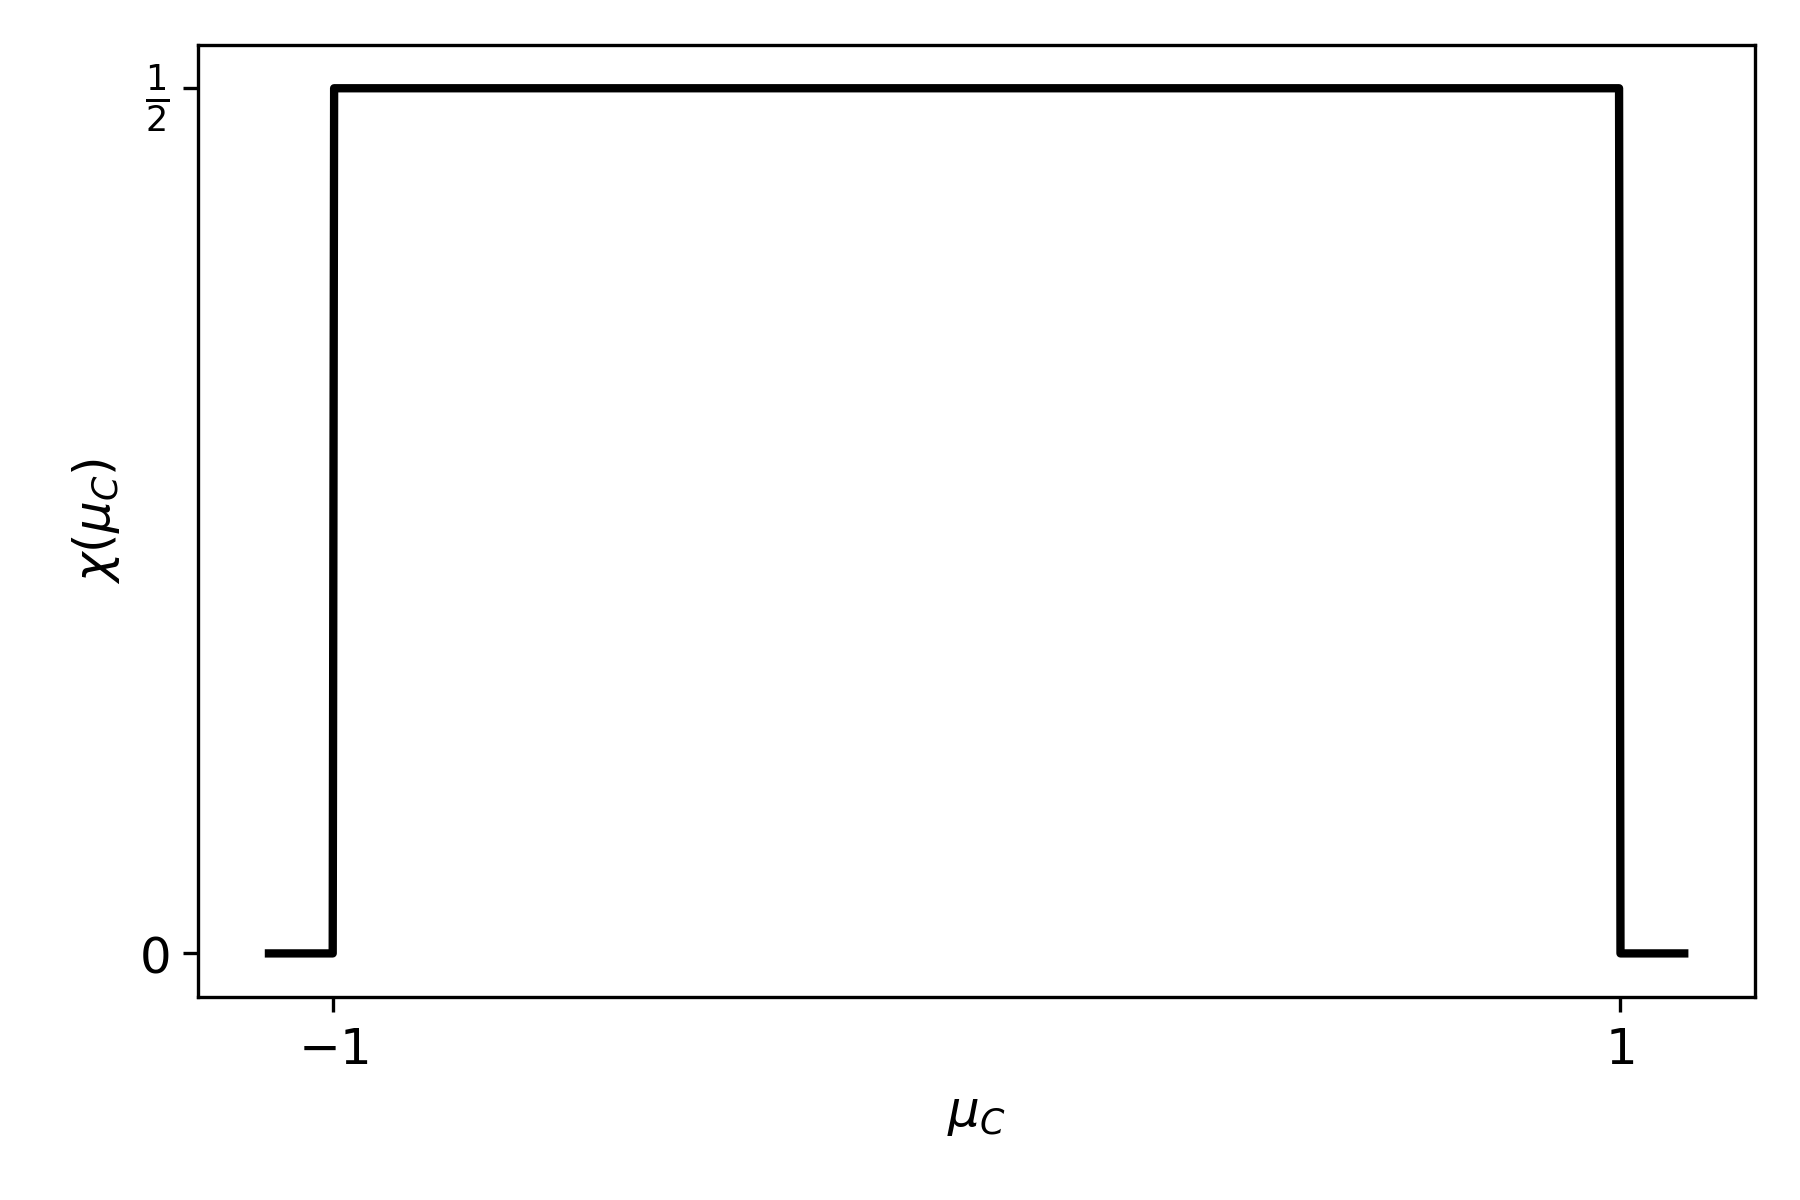
\includegraphics[scale=0.43] {figures/01-isotropmucpdf.png}
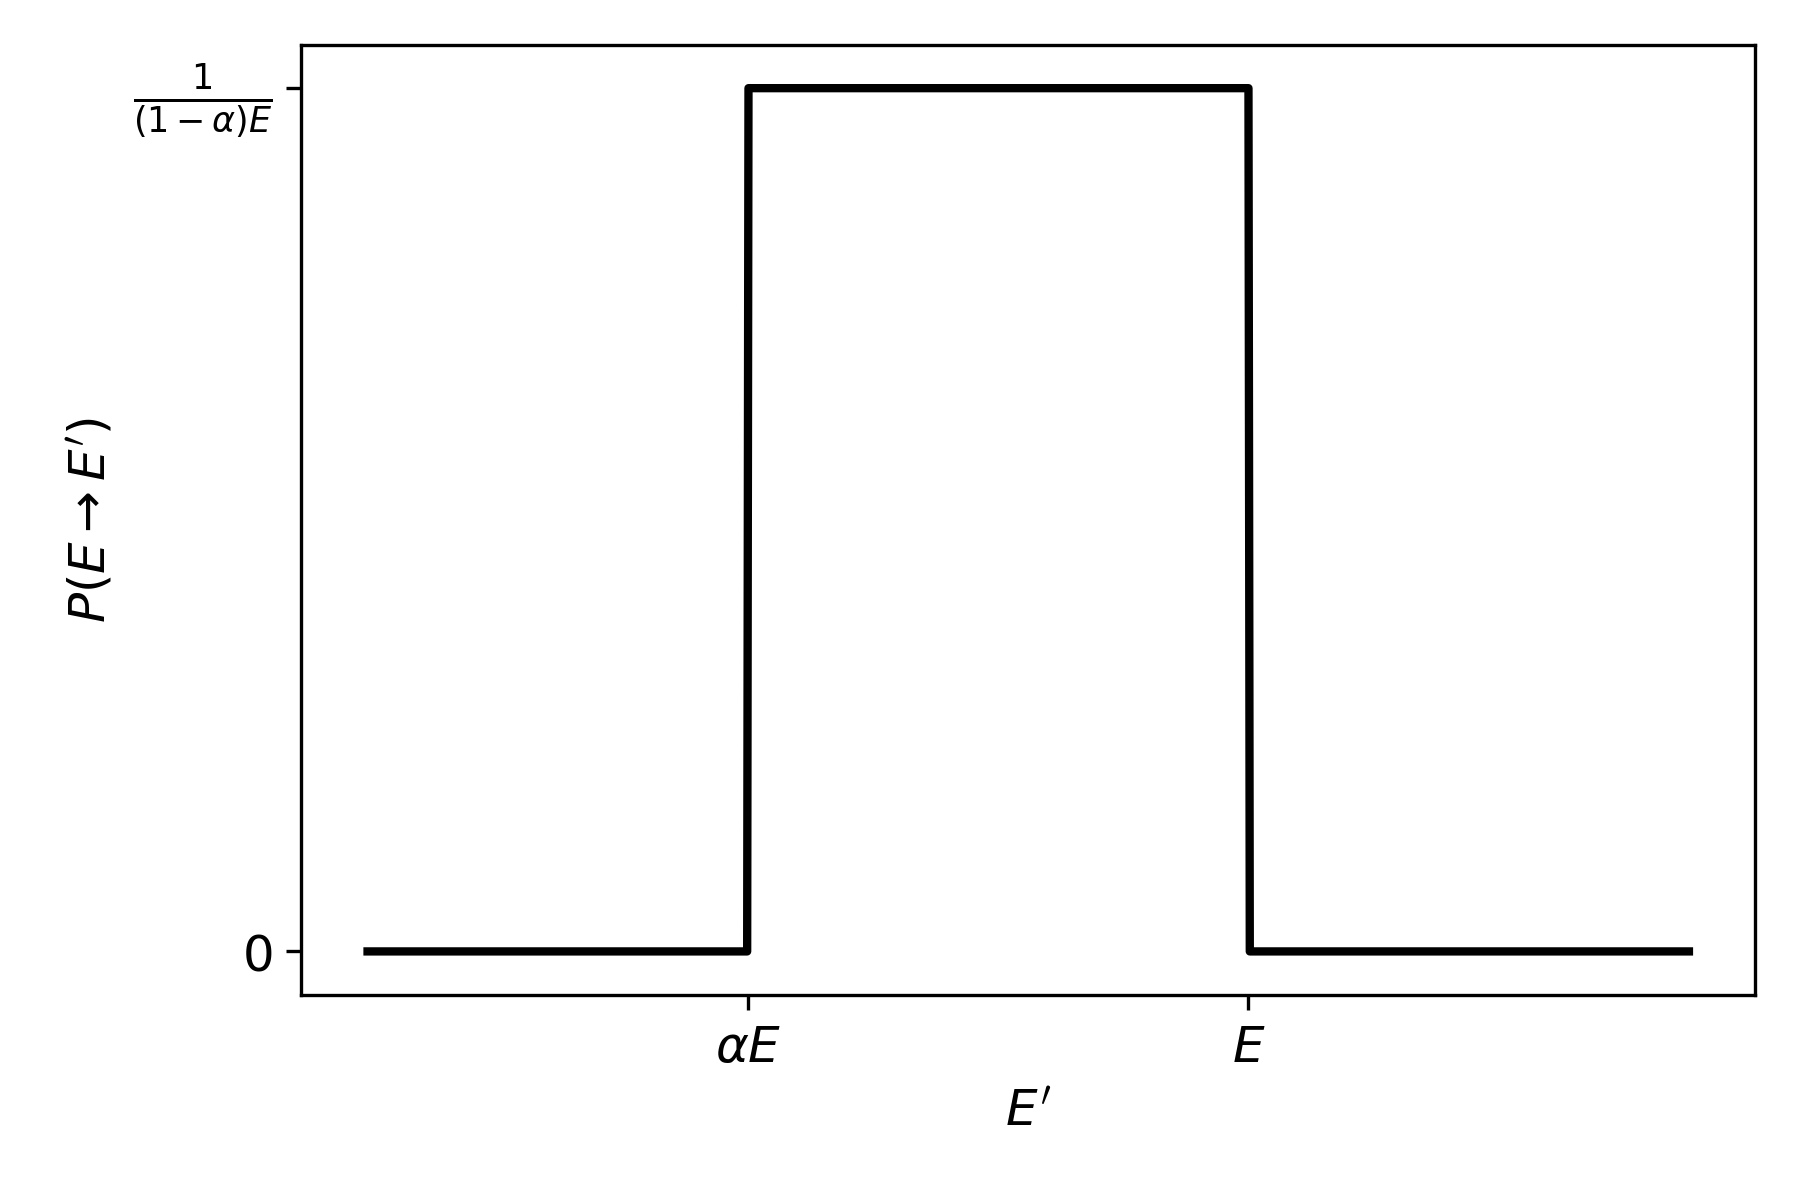
\includegraphics[scale=0.43] {figures/01-elastickernelpdf.png}}\protect
\caption{\label{fig:isotroppdf} \footnotesize{Illustration of $\chi(\mu_C)$ and $P(E\rightarrow E')$.}}
\end{figure}

Within this course we will not handle the case when elastic scattering is not isotropic in the CM. Nevertheless, as said before most often the assumption of isotropy in CM is valid at the neutron energies encountered in light water reactors. 

As we saw earlier, in fissile material the probability of fission events is much higher with low energy neutrons than with fast neutrons. Therefore, elastic scattering plays an important role in slowing down neutrons to thermal energies also materials which efficiently slow neutrons down as we will discuss in more detail in later sections. We refer to such materials as \textit{moderator}. In a light water reactor, the coolant water act as the moderator. Also, one needs to highlight again is that the energy lost by the neutron will recoil the scatterer nucleus, which leads to radiation damage. Therefore, the recoil energy is important for damage studies, although it plays little role for reactor physics.

It is also important to note that from our previous discussions we can relate the scattering angles in the CM and LAB frames by

$$\theta_L=\tan^{-1}\Big(\frac{\sin \theta_C}{\frac{1}{A}+\mu_C}\Big)$$

\noindent or as it is given in some books

$$\mu_L=\frac{A\mu_C+1}{\sqrt{A^2+2A\mu_C+1}}$$

\noindent which can be used to calculate the average scattering cosine in the LAB:

$$\bar{\mu}_L=\frac{1}{2}\int\limits_{-1}^{1}\frac{A\mu_C+1}{\sqrt{A^2+2A\mu_C+1}}d\mu_C=\frac{2}{3A}$$

\noindent which means that scattering is not isotropic in the LAB frame for light nuclei. As the mass number $A$ increases, the average cosine is converging to 0. This is important to remember, since one often only remembers that scattering is isotropic, but tends to forget that only in the CM frame. As we will see later, this will be one of the main limitations for applying diffusion theorem for the movement of neutrons, since diffusion is based on the assumption that scattering is isotropic in the LAB.


\subsection{Effects of nuclear motion}

Up to this point we have always assumed that the target is at rest. However, due to thermal motion this is not the case, nevertheless the speed of thermal motion is usually negligible compared to the neutron speed. However when the neutron energy is comparable to the thermal energy ($kT$) we need to take into account effects due to thermal motion. Neutrons having such low energies are referred to as \textit{thermal neutrons}. Typically then the neutron energy is below 1 eV.

An other important occasion when thermal motion plays a role is at resonances. A resonance has a width often less then 1 eV, therefore if slight thermal motion can have an effect on the energy dependence of the cross section around the resonance (even if the resonance occurs above thermal energies). This is called Doppler effect. 

In this text we will not derive the formalism of nuclear motion, because it is rather tedious, and the conclusions are more interesting than the way how we reached it. Proper derivations can be found in D\&H p45. The starting point of these derivations is that when calculating the interaction frequency we have to take into account the relative speed between the neutron and the nucleus:

\begin{equation}
|\textbf{v}-\textbf{V}|\sigma(|\textbf{v}-\textbf{V}|)N
\end{equation}

\noindent where the neutron moves with velocity $\textbf{v}$ and the nucleus moves with velocity $\textbf{V}$. Then in the next step one needs to acknowledge, that not all nuclei move with the same velocity, instead one needs to take into account a distribution for the nucleus velocity and at the end one can arrive to a thermally averaged cross section. If that is then applied on  resonances one could observe the behavior illustrated in Figure \ref{fig:doppler}: the resonance broadens while its peak decreases with increasing temperature. Therefore this is often called Doppler-broadening. As we will see, later, although the integral under the resonance is unchanged due to increasing temperature, still the probability of neutrons being absorbed by the resonance increases, because while neutrons loose their energy there is an increasing probability that they encounter the nucleus at the resonance energy. Therefore Doppler-broadening has an important safety implication: with increasing temperatures the number of neutrons (therefore the power) decreases.

\begin{figure}[ht!]
\protect \centering{
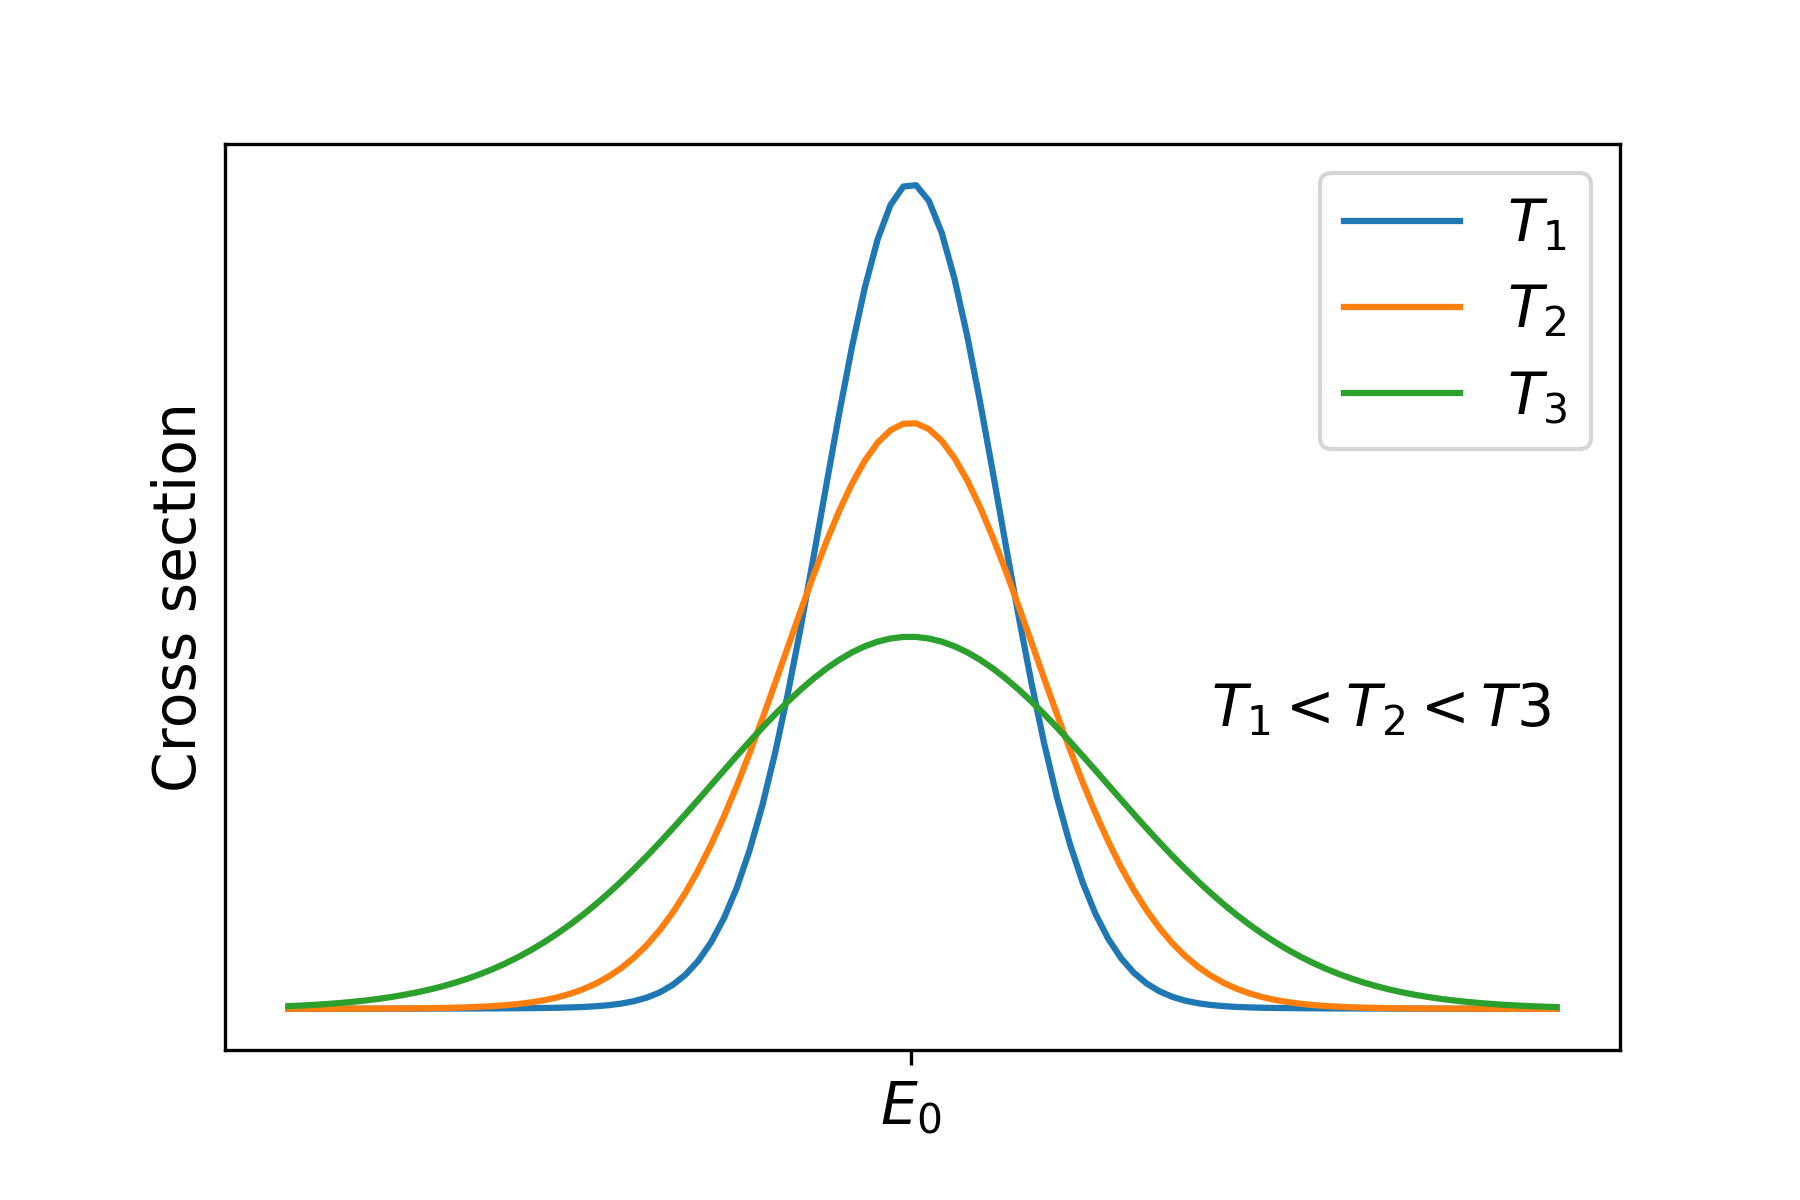
\includegraphics[scale=0.46] {figures/01-doppler.png}}\protect
\caption{\label{fig:doppler} \footnotesize{Doppler broadening of resonances.}}
\end{figure}

Another noteworthy impact of nuclear motion is for the differential scattering cross section. The derivation of such scattering kernel is an enormous task, the interested reader can find joy in reading M. M. R. Williams:  The Slowing Down and Thermalization of Neutrons (freely available from OECD NEA). For us now again mostly the conclusion, illustrated in Figure \ref{fig:thermalkernel} is of interest. At thermal energies, the neutron in fact can gain energy from a scattering event. This is called \textit{upscattering}. We can see that with increasing the energy of the incoming neutron the scattering kernel becomes the uniform distribution we have derived before, however for lower energy neutrons upscattering is more and more probable. Such scattering kernel can be given as


\begin{equation}
\begin{aligned}
\sigma_s(E'\rightarrow E)=\frac{\sigma_s}{2E'}\eta^2\Bigg[\text{erf}\Bigg(\eta\sqrt{\frac{E}{kT}}-\rho\sqrt{\frac{E'}{kT}}\Bigg)\pm \text{erf}\Bigg(\eta\sqrt{\frac{E}{kT}}+\rho\sqrt{\frac{E'}{kT}}\Bigg)\Bigg]+ \\ \frac{\sigma_s}{2E'}\eta^2\exp\Bigg(-\frac{E-E'}{kT}\Bigg)\Bigg[\text{erf}\Bigg(\eta\sqrt{\frac{E'}{kT}}-\rho\sqrt{\frac{E}{kT}}\Bigg)\mp \text{erf}\Bigg(\eta\sqrt{\frac{E'}{kT}}+\rho\sqrt{\frac{E}{kT}}\Bigg)\Bigg]
\end{aligned}
\end{equation}

\noindent where

\[
\eta=\frac{A+1}{2\sqrt{A}} \quad \text{and} \quad \rho=\frac{A-1}{2\sqrt{A}}
\]

\noindent and the upper sign is for $E\leq E'$, and the lower sign is for $E\geq E'$.

\begin{figure}[ht!]
\protect \centering{
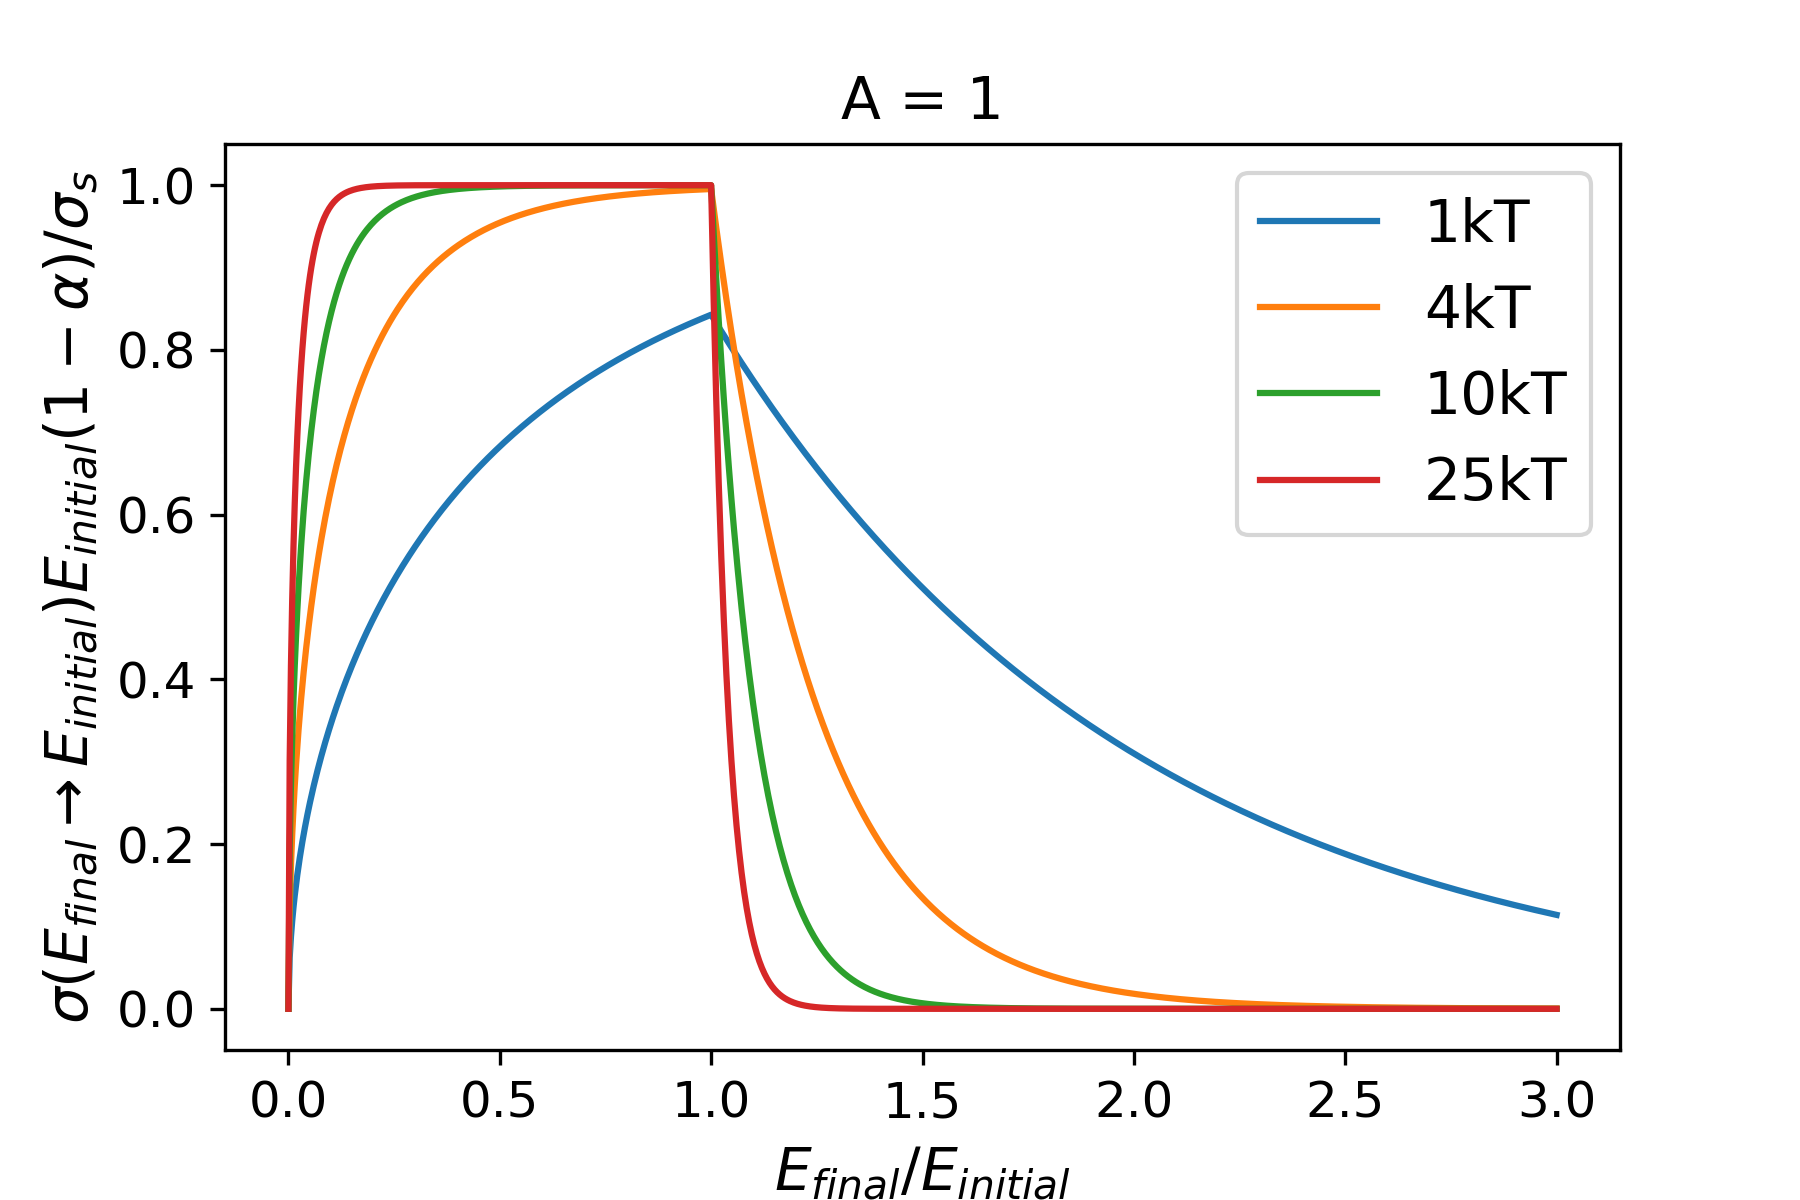
\includegraphics[scale=0.46] {figures/01-thermalscatteringkernel1.png}
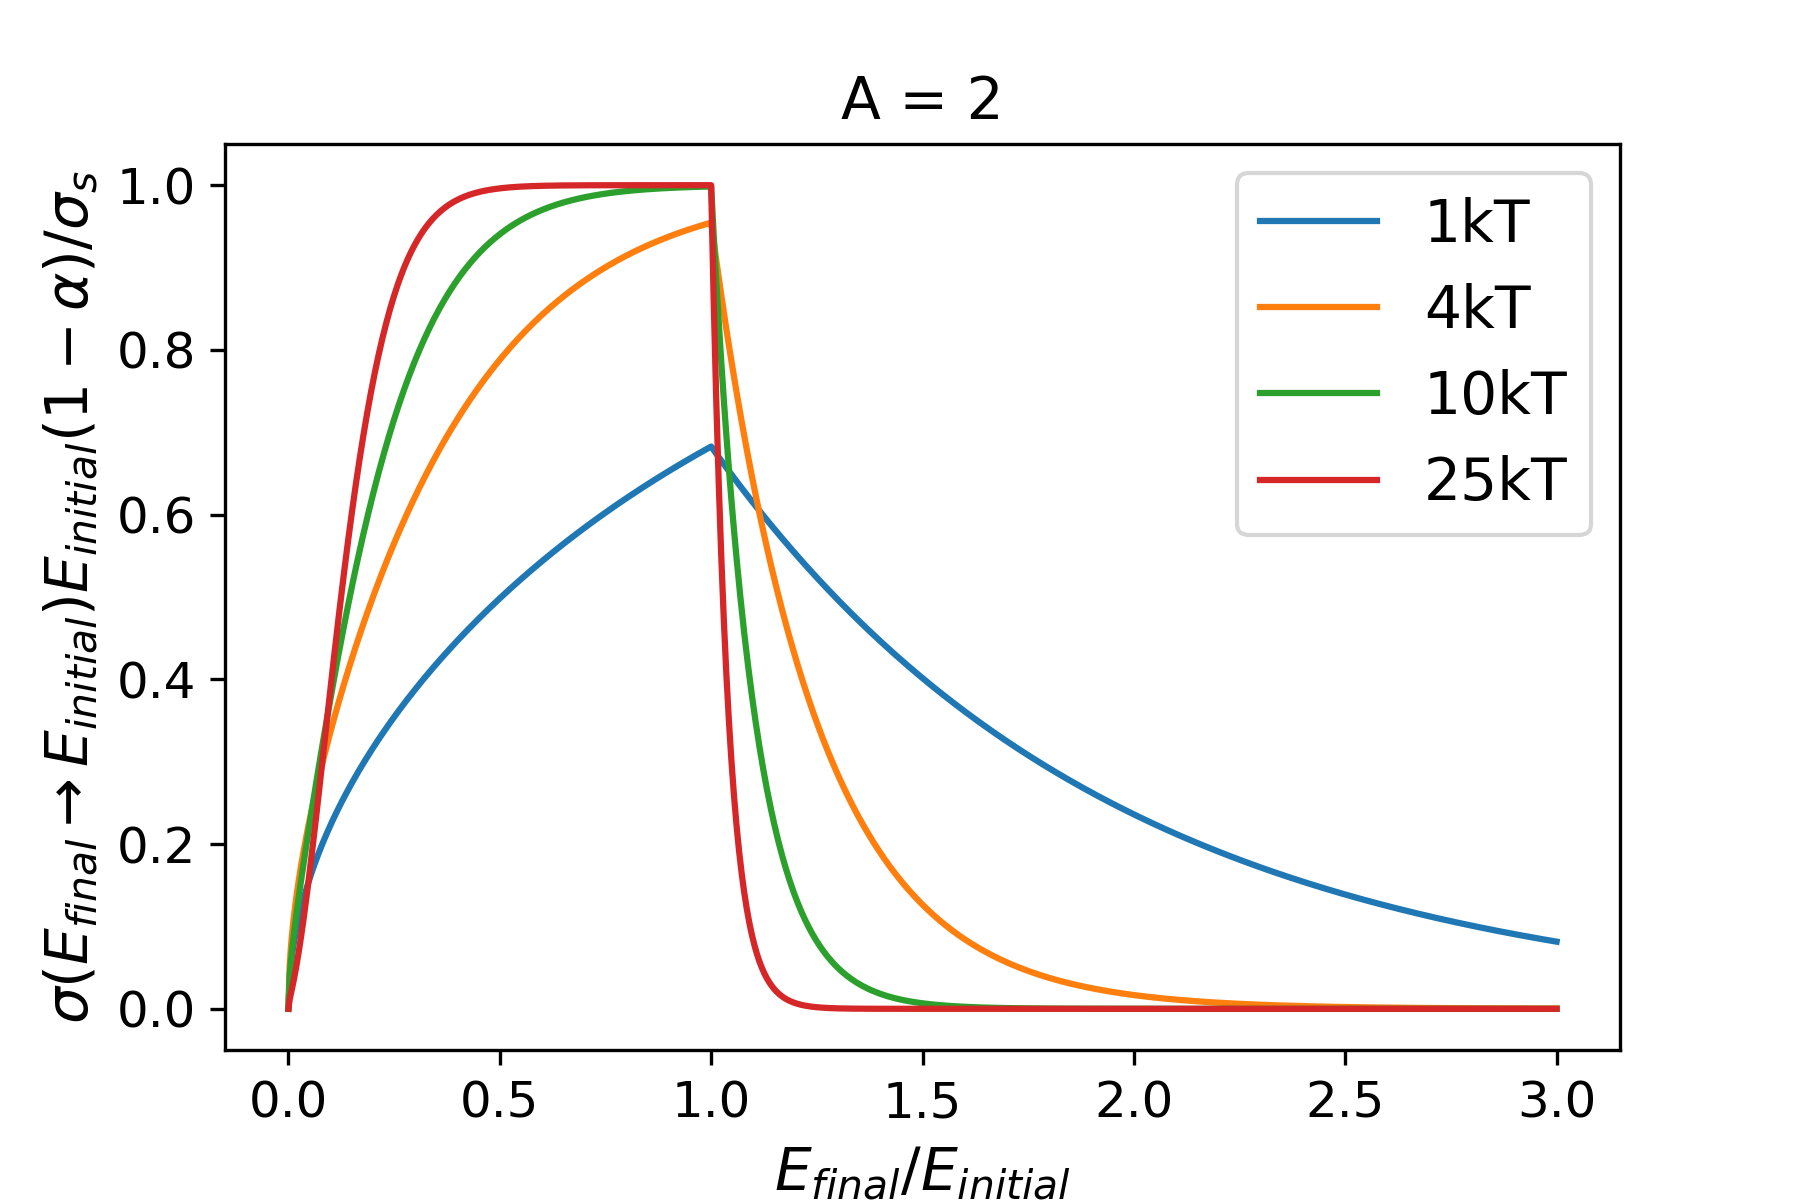
\includegraphics[scale=0.46] {figures/01-thermalscatteringkernel2.png}
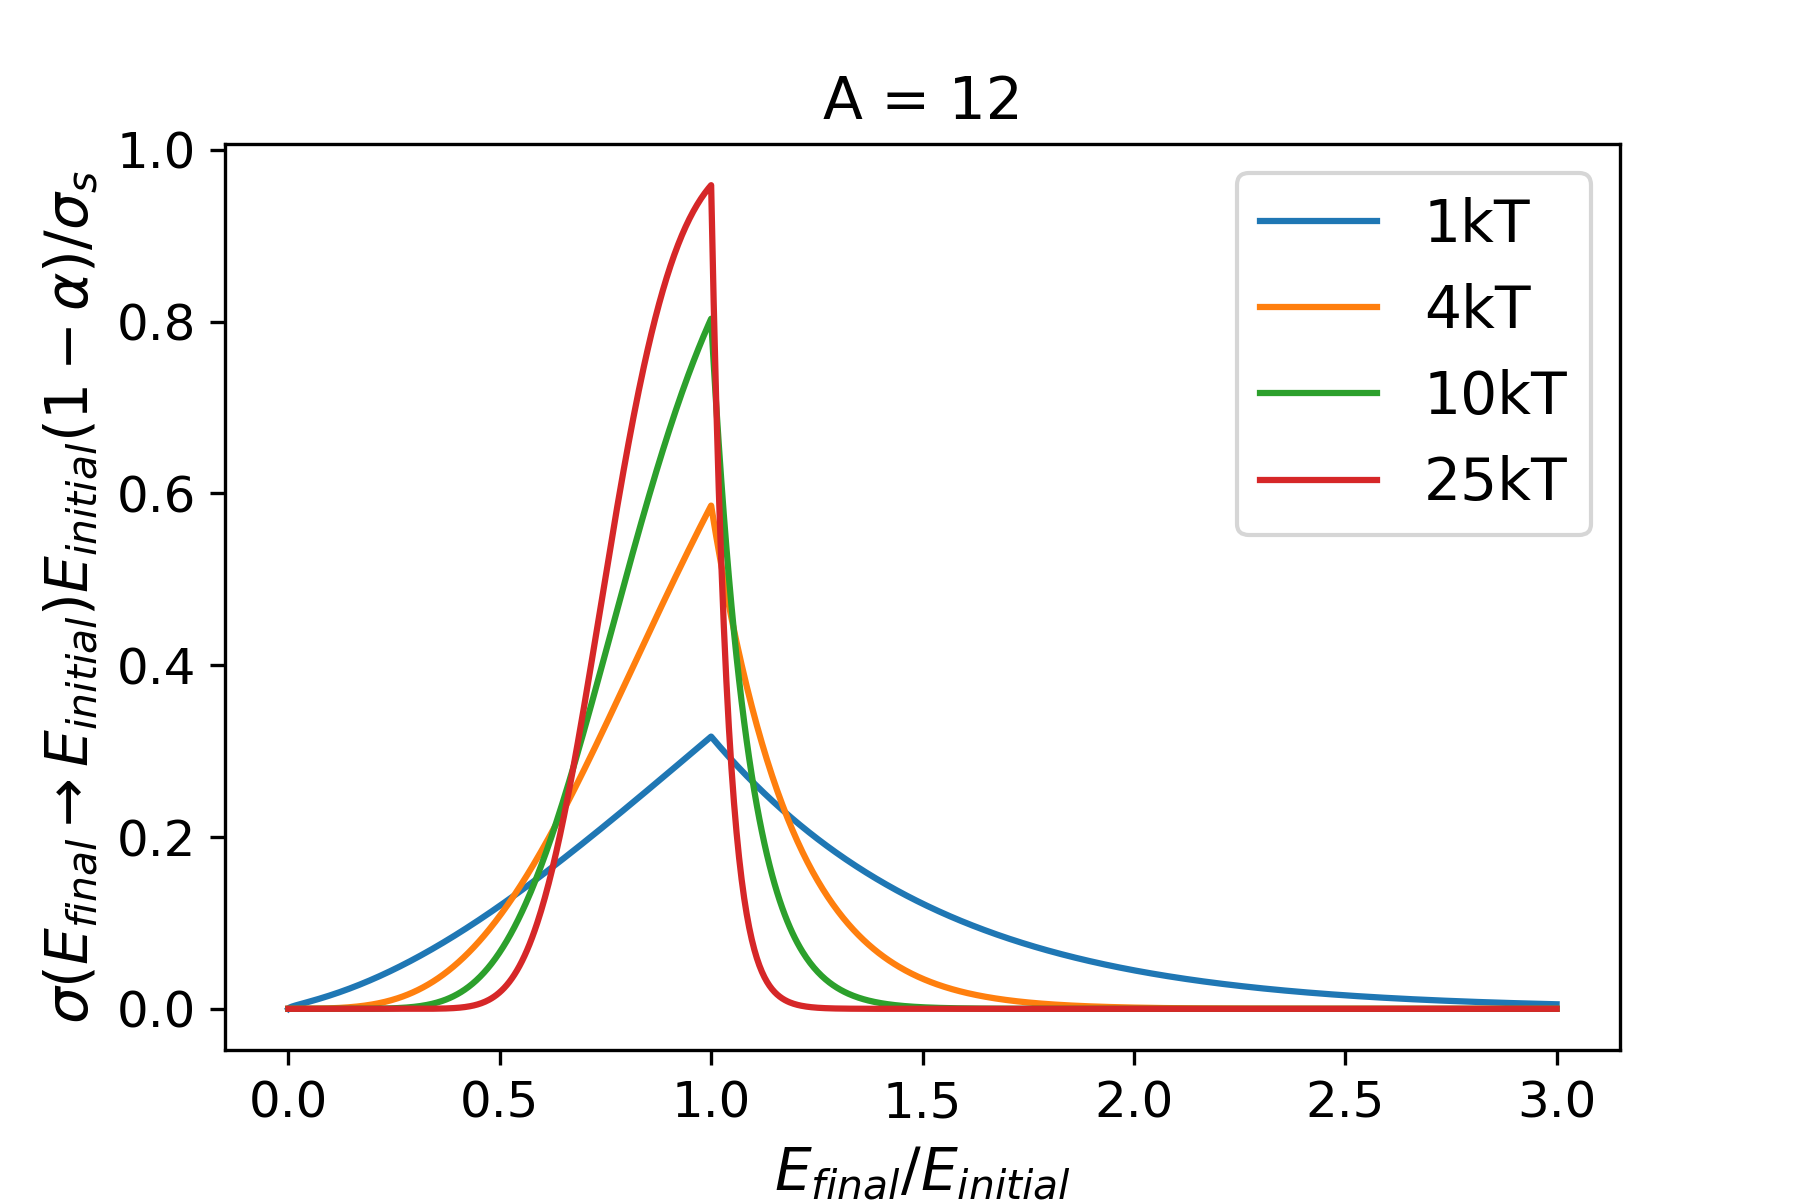
\includegraphics[scale=0.46] {figures/01-thermalscatteringkernel12.png}}\protect
\caption{\label{fig:thermalkernel} \footnotesize{Thermal scattering kernel.}}
\end{figure}

\subsection{Impact of molecular bounds}

Without going into details, it has to be mentioned that chemical bounds and crystal structures also influence scattering kinematics of thermal neutrons. This is relevant in reactor physics, since the scattering hydrogen atoms are bounded in water, which is used as the coolant and moderator of LWRs. Usually special tables are created and used that account for thermal binding effects. These are called $S(\alpha,\beta)$ tables. The theory behind the $S(\alpha,\beta)$ formalism roots in quantum mechanics, and the previously mentioned book of Williams provides a more detailed description for the interested reader. The only implication for us will be that in Monte Carlo calculations we will need to link to such tables when including materials like water in our problem.


\subsection{Nuclear fission}

Fig. \ref{fig:binding} shows that the average binding energy per nucleon has a maximum at Ni-62. Therefore fusing lighter nuclei or splitting (fissioning) heavier nuclei can lead to tighter bound nuclei, and the difference of binding energy is released in the form of energy. The main goal of building nuclear reactors is to extract the energy released during the fissioning of heavy nuclei. The reason that heavier nuclei undergo fission spontaneously only with a low probability is that the short range nuclear forces give rise to a potential energy barrier (or fission barrier), which usually has a height of 6-9 MeV. 

In order to overcome this barrier first some energy needs to be supplied to the nucleus:

\begin{enumerate}
\item by an energetic particle, for example a $\gamma$ photon (photofission)
\item by capturing a neutron to cover the energy with the binding energy of the neutron
\item by combining 1. and 2.: capturing a fast neutron
\item seldom fission can happen due to quantum mechanical tunneling (spontaneous fission)
\end{enumerate}

Nuclides which can fission by capturing slow neutrons are called \textit{fissile} (eg. U235, Pu239), wheras nuclices which have too high fission barriers therefore undergo fission only with fast neutrons are called \textit{fissionable} (eg. U238, Pu240). Recall, that for these nuclides the fission cross section presets a threshold energy, below which the probability of fission is almost negligible and the cross section is several orders of magnitude lower (eg. the fission cross section of U-238 in Fig. \ref{fig:ufission}).

It is however possible that after the neutron absorption of a nucleus the compound nucleus decays to its ground state, thus the neutron is lost for the chain reaction. The relative balance of capture and fission can be described by the 

\begin{equation}
\textit{capture-to-fission ration}=\frac{\sigma_c}{\sigma_f}
\end{equation}

of a given nuclide. This ratio of course does depend on the energy of the incoming neutron.

A typical fission reaction look as 

\[
n+{}_{92}^{235}U\rightarrow {}_{92}^{236}U^* \rightarrow \text{fission reaction products}
\]

where the reaction products cover a wide variety of particles and carry cca 200 MeV energy:

\begin{itemize}
\item charged and energetic fission products (nuclei with medium mass number), which quickly slow down in the surrounding media (while picking up electrons), and loosing their energy.
\item several neutrons with large kinetic energy
\item $\gamma$ photons
\item $\beta$ particles and neutrinos from the decay of fission products
\end{itemize}

The fission products has a distribution given by the fission yield (ie. probability) of the nuclide created in fission. In fission the nucleus is usually split asymmetrically, therefore the fission yield curve has two distinct peaks as shown in Fig. \ref{fig:fissyield}. With lower probability the nucleus can split into three fission products (ternary fission), when a third, light nuclide (eg. H-3) is created. In the top figure we can see a small "island" of light nuclides which are the result of ternary fission. The fission yield depends both on the ingoing neutron energy (and is usually tabulated separately for thermal and for fast neutrons) and on the target nuclide.

\begin{figure}[ht!]
\protect \centering{
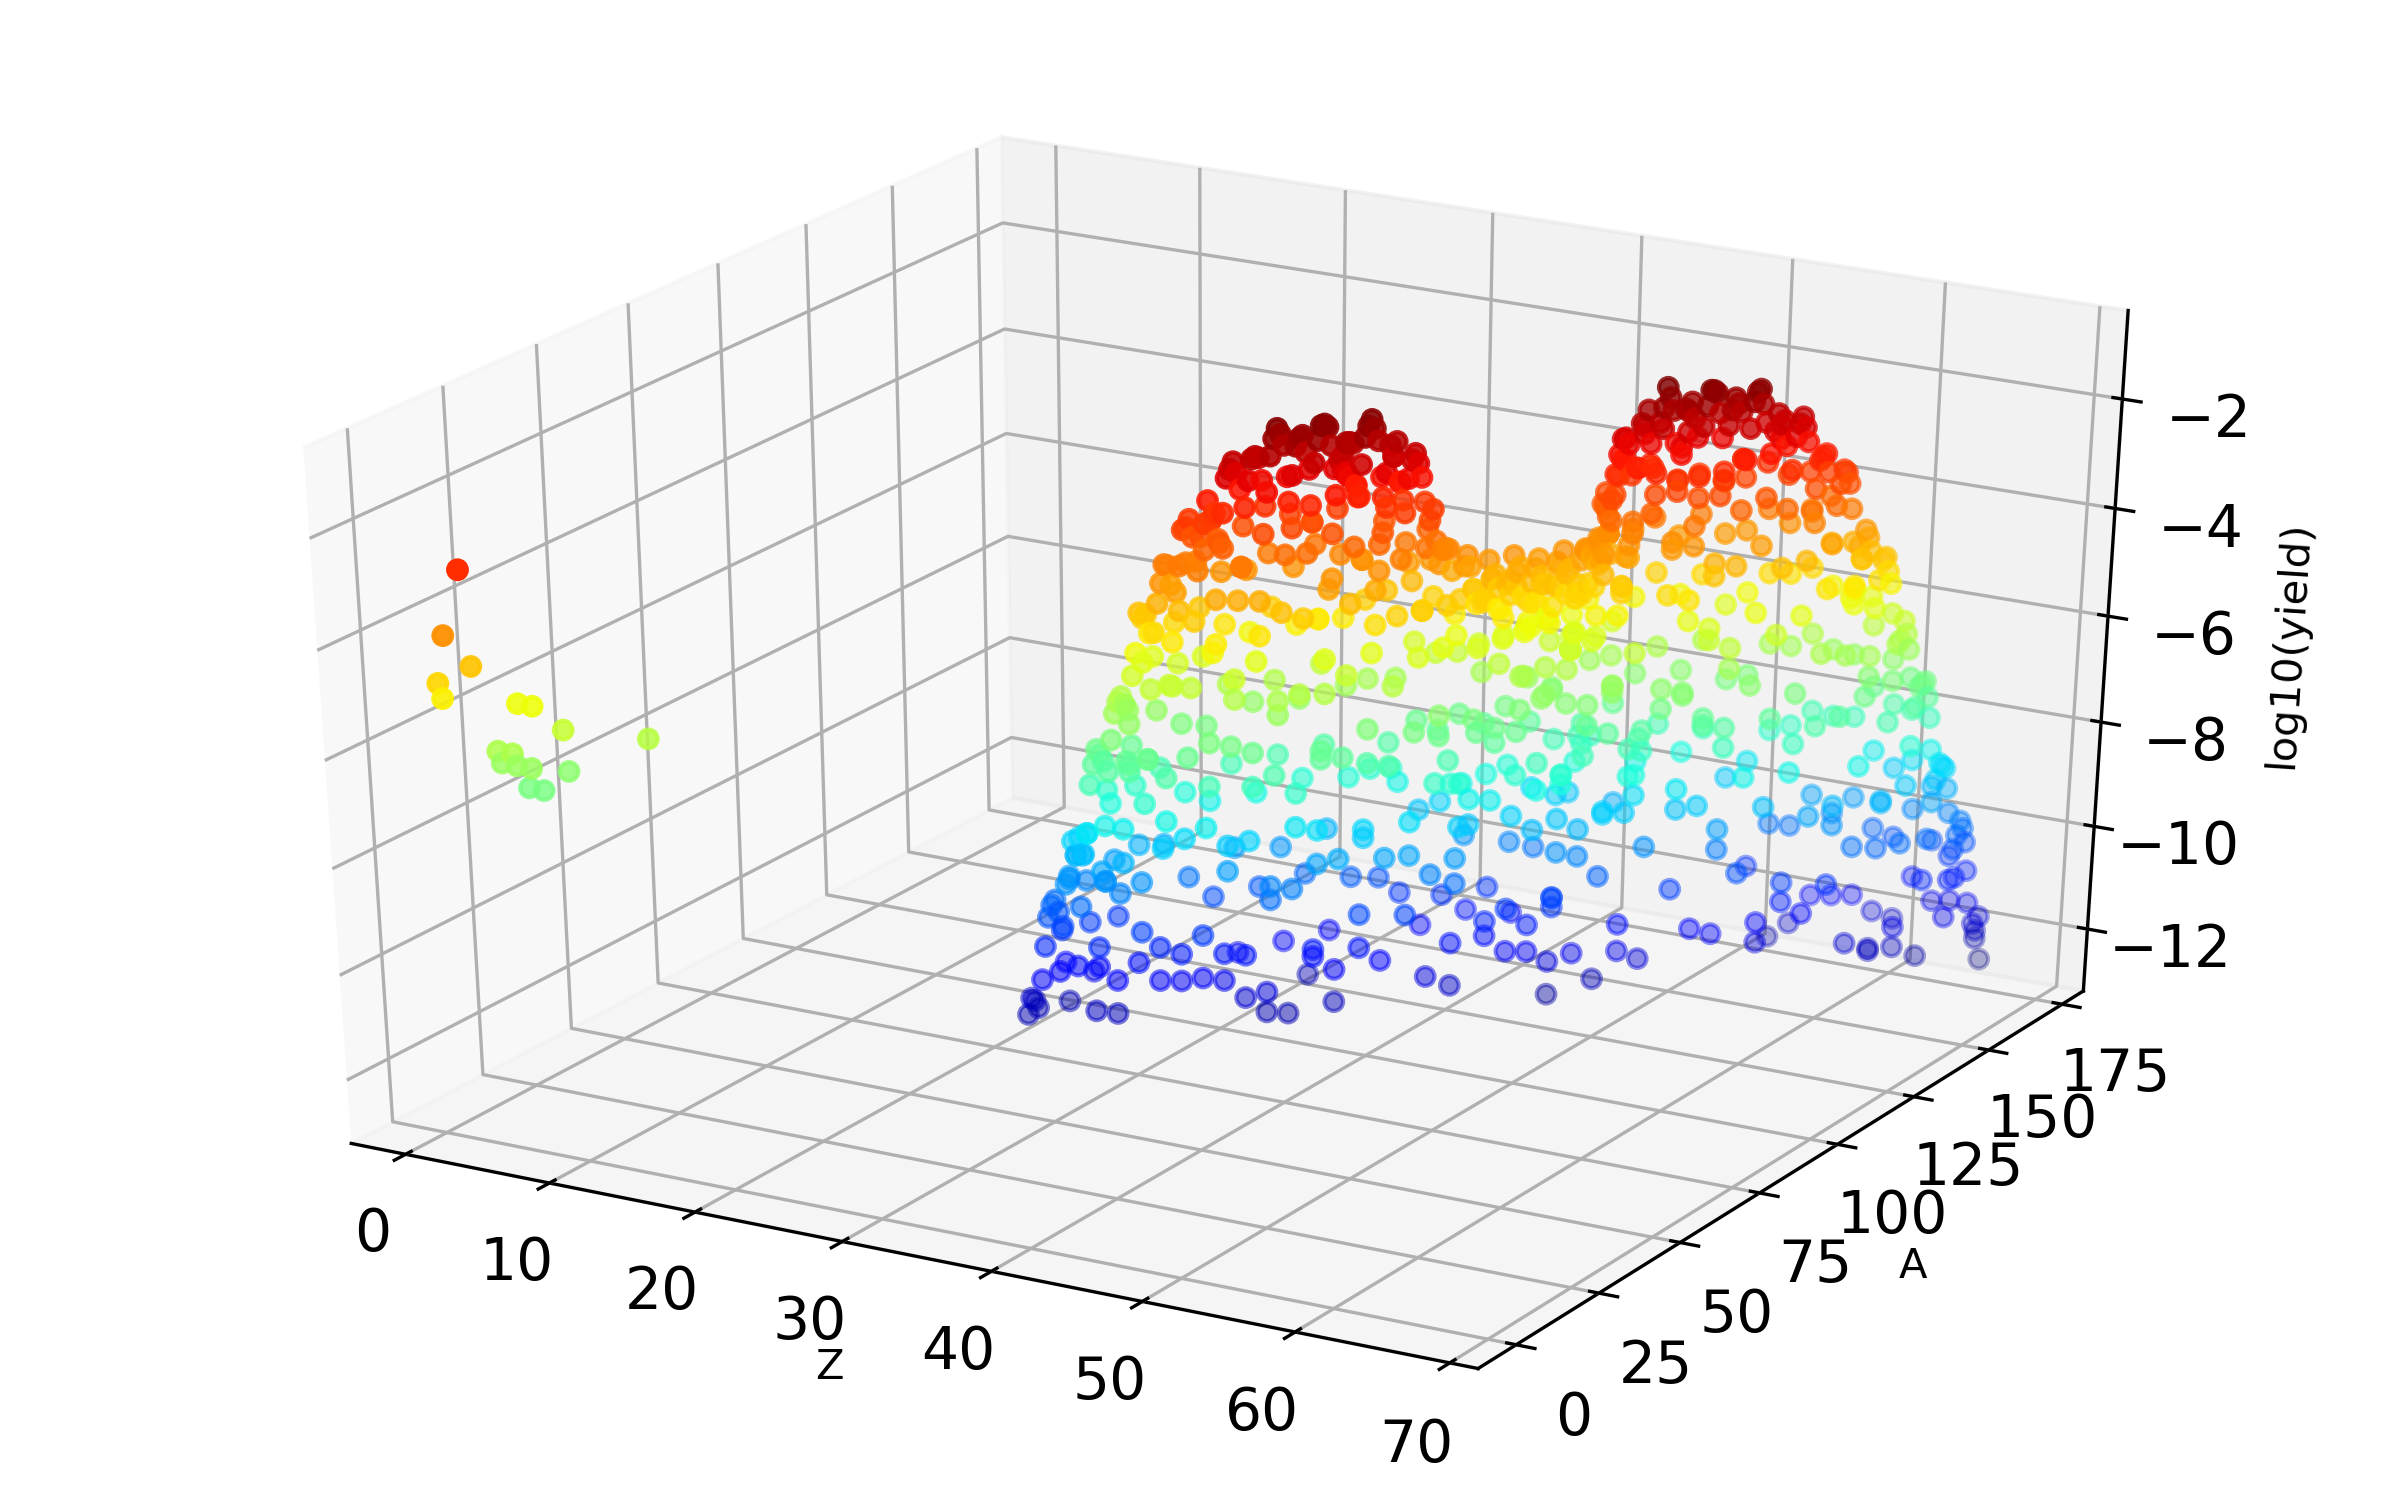
\includegraphics[scale=0.46] {figures/01-fissionyield3d-U235.png}
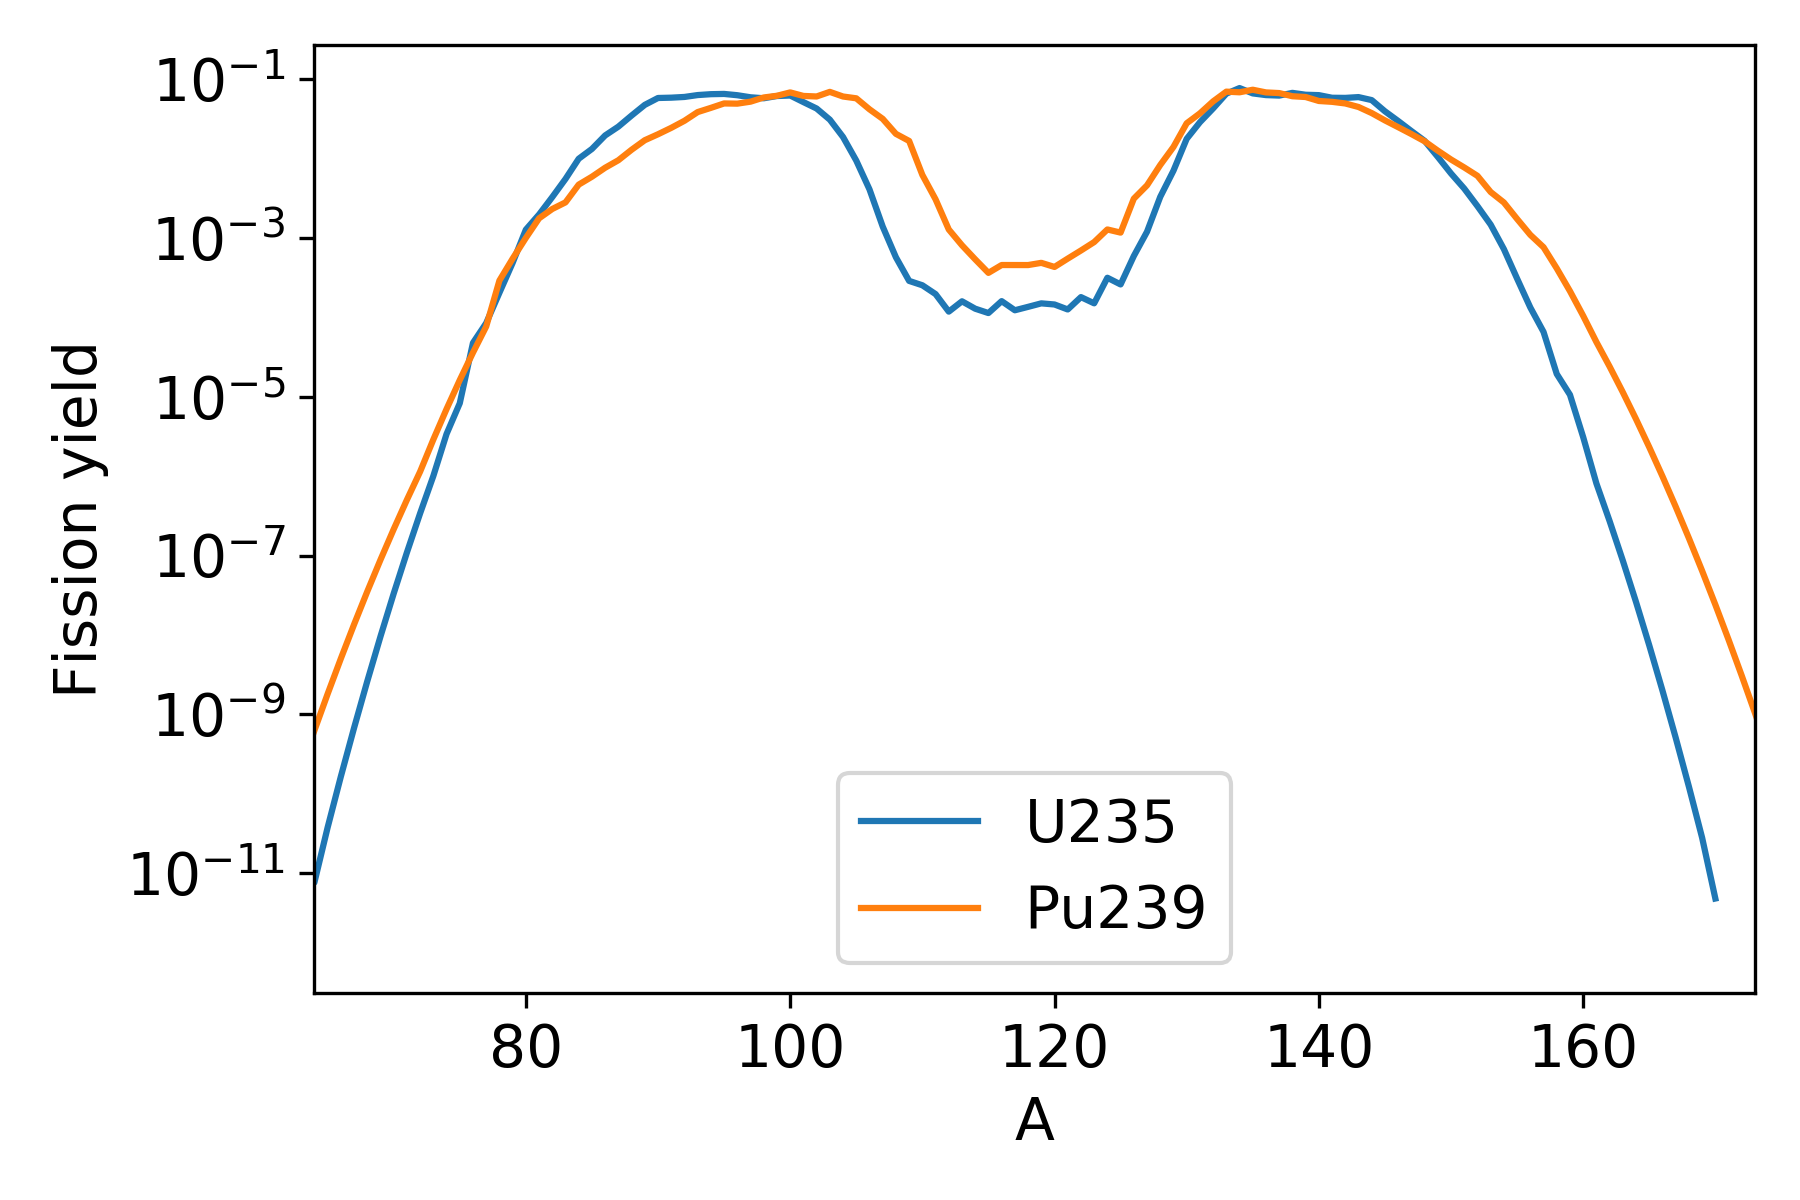
\includegraphics[scale=0.46] {figures/01-fissionyield2d.png}}\protect
\caption{\label{fig:fissyield} \footnotesize{Top: fission yield of U-235. Bottom: fission yield of U-235 and Pu-239 (both for thermal neutrons)}}
\end{figure}

Since the fission products are typically neutron rich, they undergo $\beta$-decay, thus around 4-5\% of the energy is released in the form of radioactive decay with a time delay. A reactor core needs to be designed to be so that this decay heat can be removed from the system after the reactor is shutdown. The distribution of energy and where it is absorbed is given by the table below.

\begin{table}\caption{Distribution of energy in fission.}
\begin{tabular}{c | c | c | c}
Product & Energy (\%) & Range & Time delay \\
\hline
Fission product & 80 & short & prompt \\
Fast neutron & 3 & medium & prompt \\
Fission $\gamma$ & 4 & medium & prompt \\
$\beta$ decay & 4 & short & delayed \\
neutrinos & 5 & long & delayed \\
Non fission reactions & 4 &  & delayed 
\end{tabular}
\end{table}

Out of these events the short range events typically deposit the energy within the region the fission happened (ie. in the rod), therefore we need continuous cooling of the rods. Some of the energy is deposited farther from the source location (in the coolant, or in the shielding). As mentioned before the delayed component due to the radioactive decay of fission products requires the fuel to be cooled after the fission chain reaction is stopped in the reactor.

From the fission event several neutrons can be emitted, as we already discussed briefly, and soon will discuss in more detail, these neutrons make it possible to create a self-sustaining chain reactions, with the neutrons being chain carriers. Most of these neutrons are emitted almost instantaneously (within $10^{-14}$ s which is negligible compared to the time scales of neutron reactions), and are called prompt. But a small portion of neutrons (cca 0.6 \%) is emitted with a time delay.

The number of emitted neutrons (often noted with the greek letter $\nu$, and the average number as $\bar\nu$) varies between 0 and 6, with the most probable event being the emission of 2-3 neutrons as shown in Fig. \ref{fig:nu} for U-235. This distribution depends both on the nuclide and on the neutron energy. However, as one can see in the lower figure, the nubar is essentially constant for energies and nuclides relevant in light water reactors.

\begin{figure}[ht!]
\protect \centering{
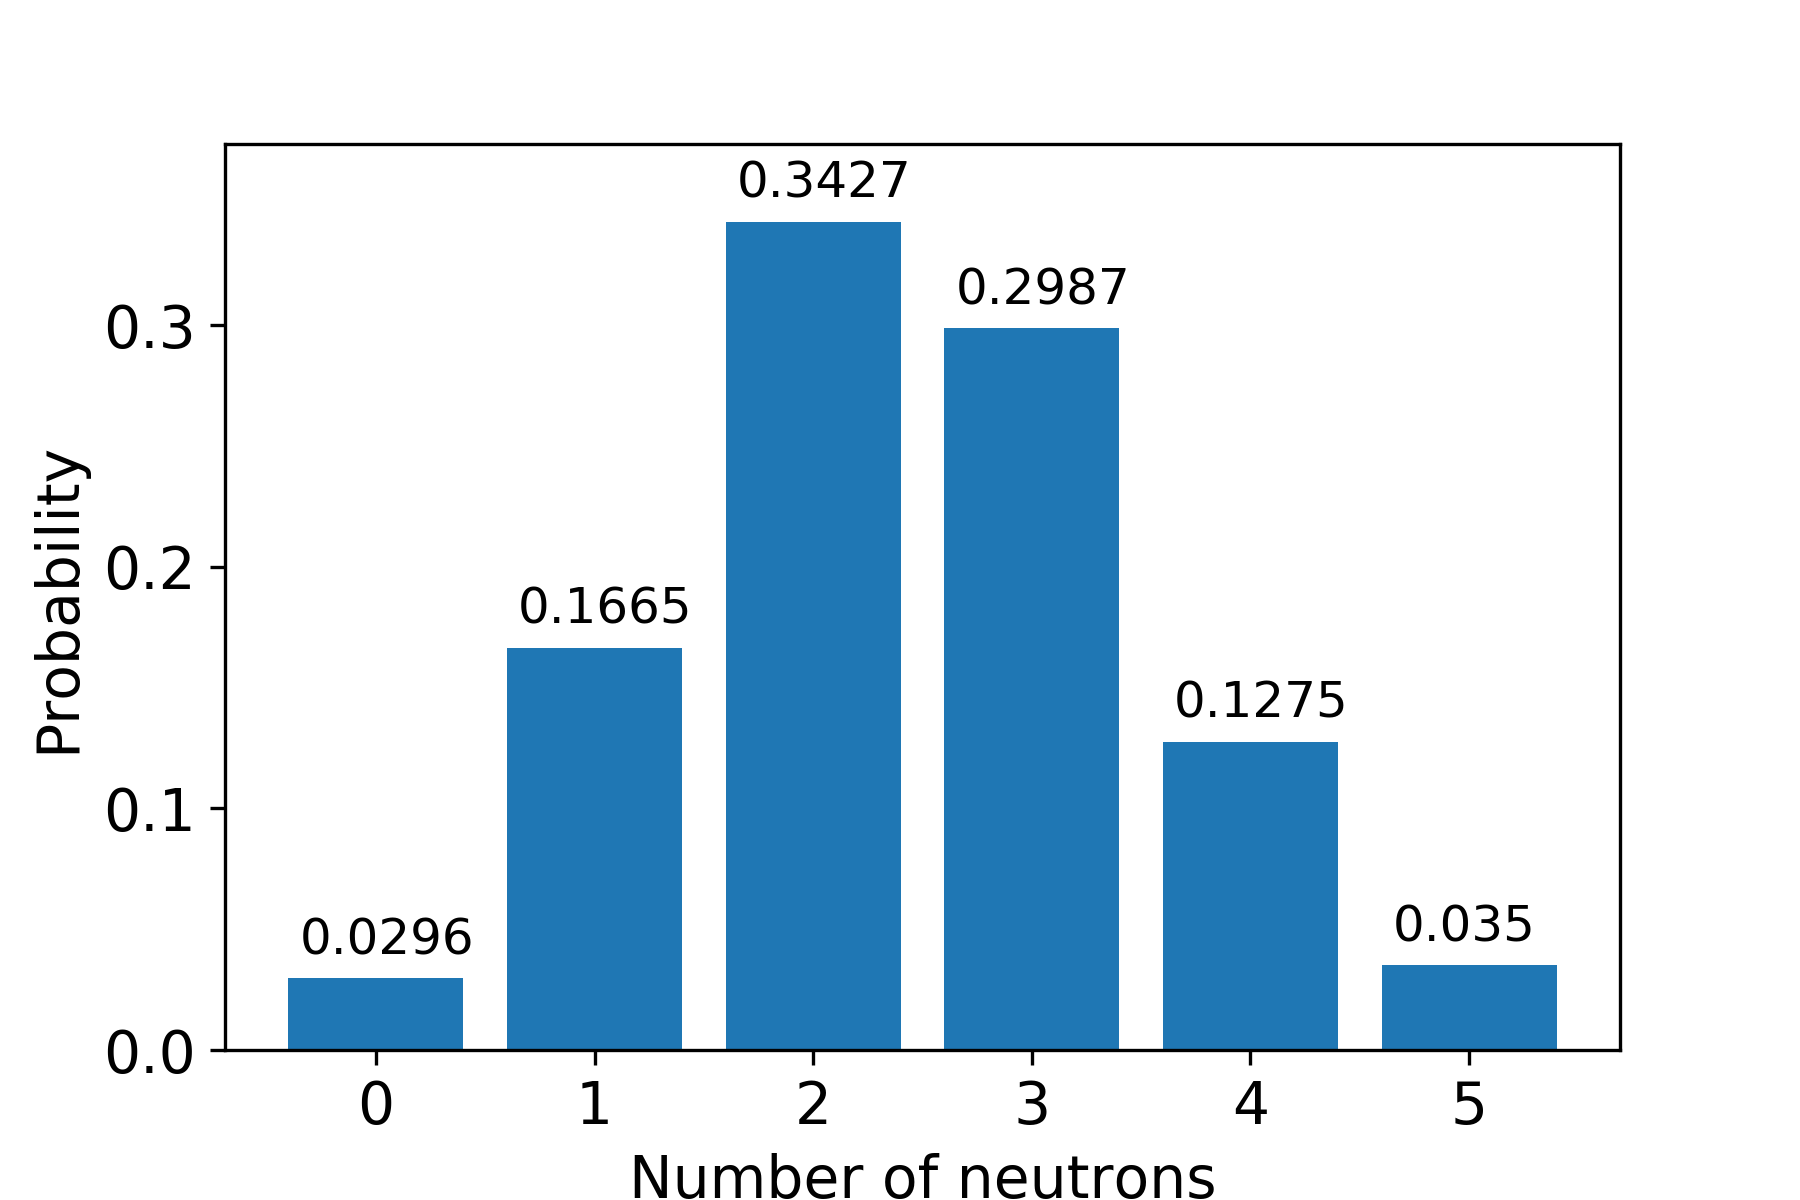
\includegraphics[scale=0.46] {figures/01-nu.png}
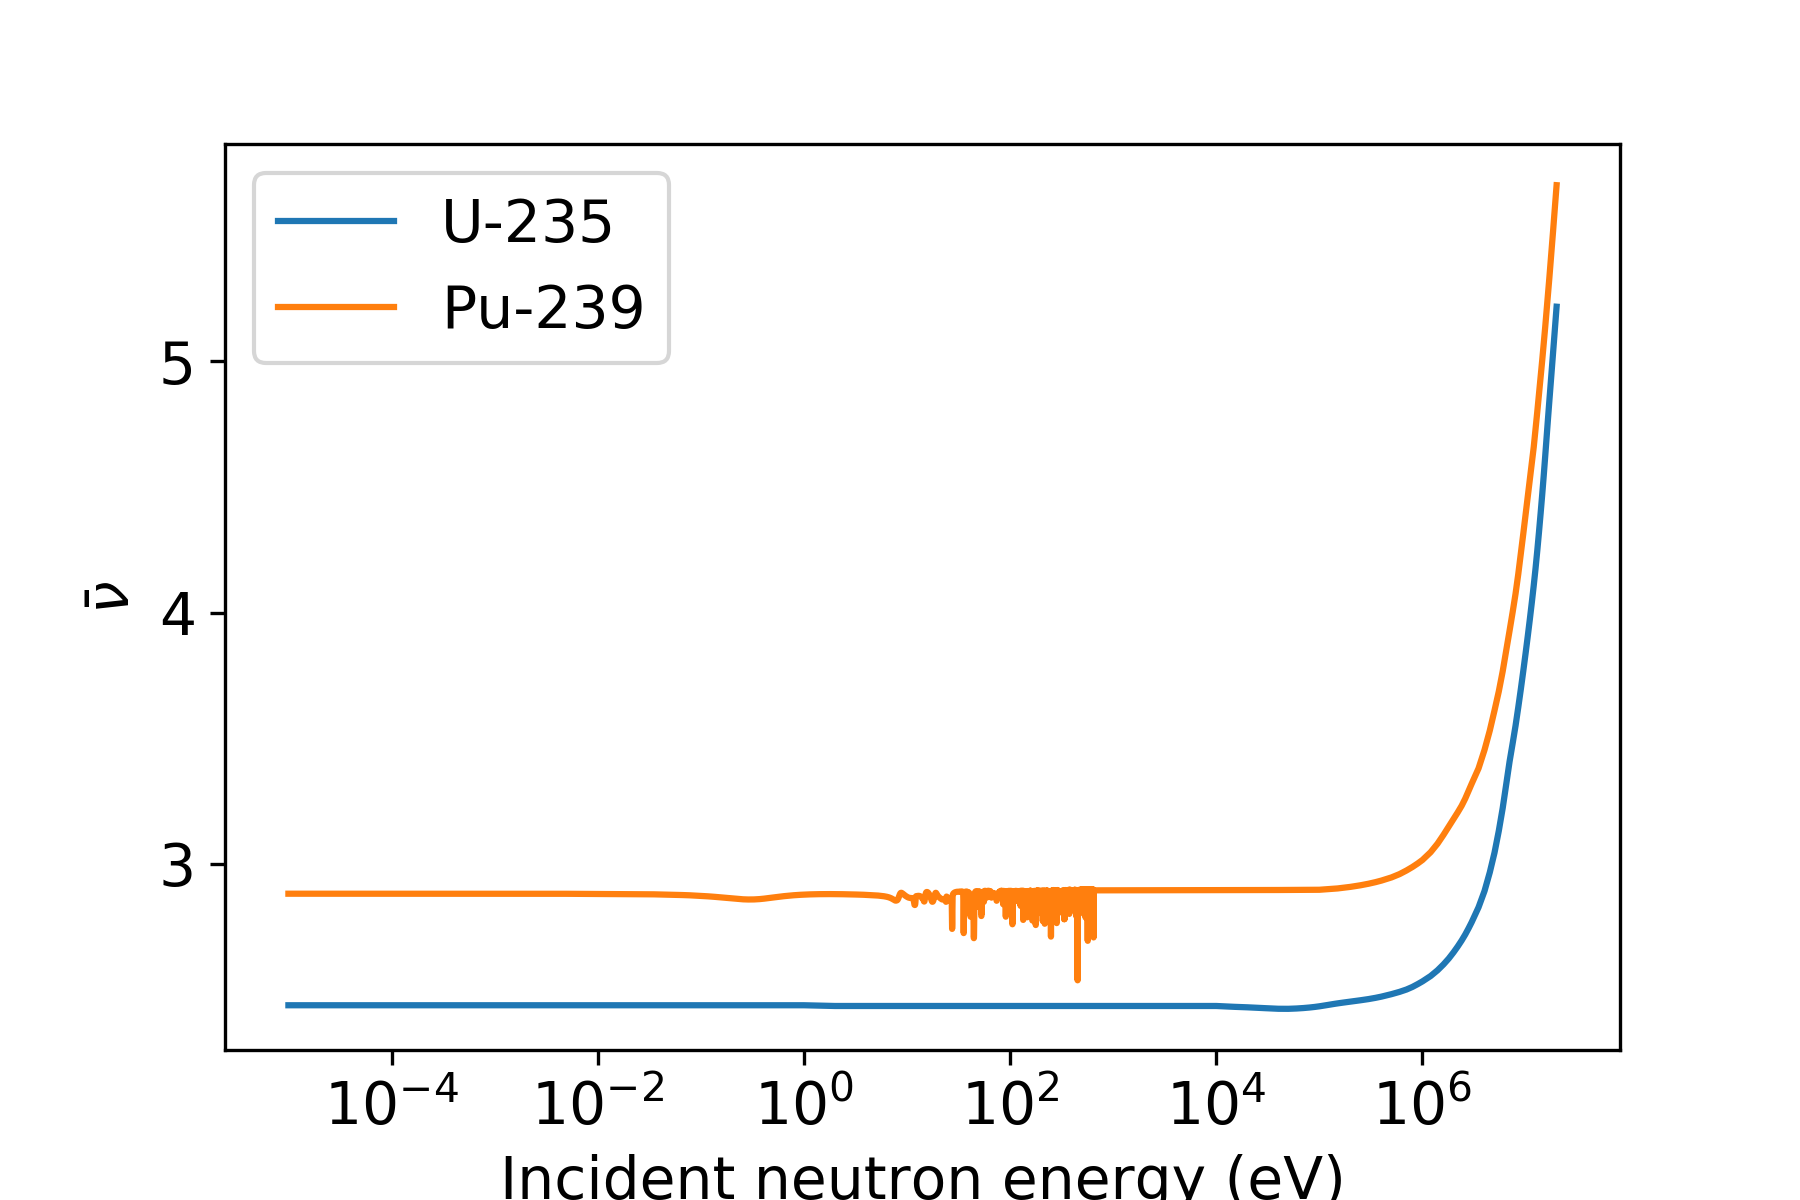
\includegraphics[scale=0.46] {figures/01-nubar.png}}\protect
\caption{\label{fig:nu} \footnotesize{Top: Number of emitted neutrons in the thermal fission of U-235. Bottom: Nubar of U-235 and Pu-239 vs the ingoing neutron energy.}}
\end{figure}

The energy distribution of the prompt fission neutron can be described by the semi-empirical Watt-spectrum 

\begin{equation}
\chi(E)=C_1\cdot \exp(-\frac{E}{C_2})\cdot \sinh(\sqrt{C_3\cdot E})
\end{equation}

\noindent where   $C_1 = 0.453$, $C_2 = 0.965$ and $C_3 = 2.29$ for U-235. $\chi(E)dE$ is the probability that the neutron after birth will have an energy between $[E,E+dE]$. The most probable neutron energy is cca. 0.85 MeV, and the average energy is 2 MeV. One can also observe from Fig. \ref{fig:watt} that birth neutron energies above 5 MeV are less probable, therefore in the future we can neglect some reactions, such as $(n,\textit{i}n)$ reactions which only happen with high energy neutrons). The birth energy spectrum is rather independent from the ingoing neutron energy, and is similar for most of the nuclides. For very detailed calculations one can take into account an event-by-event sampling of the birth energy (for example by taking into account that neutrons emitted from the same fission event have slightly correlated energies), but for us this simple model suffices. 

\begin{figure}[ht!]
\protect \centering{
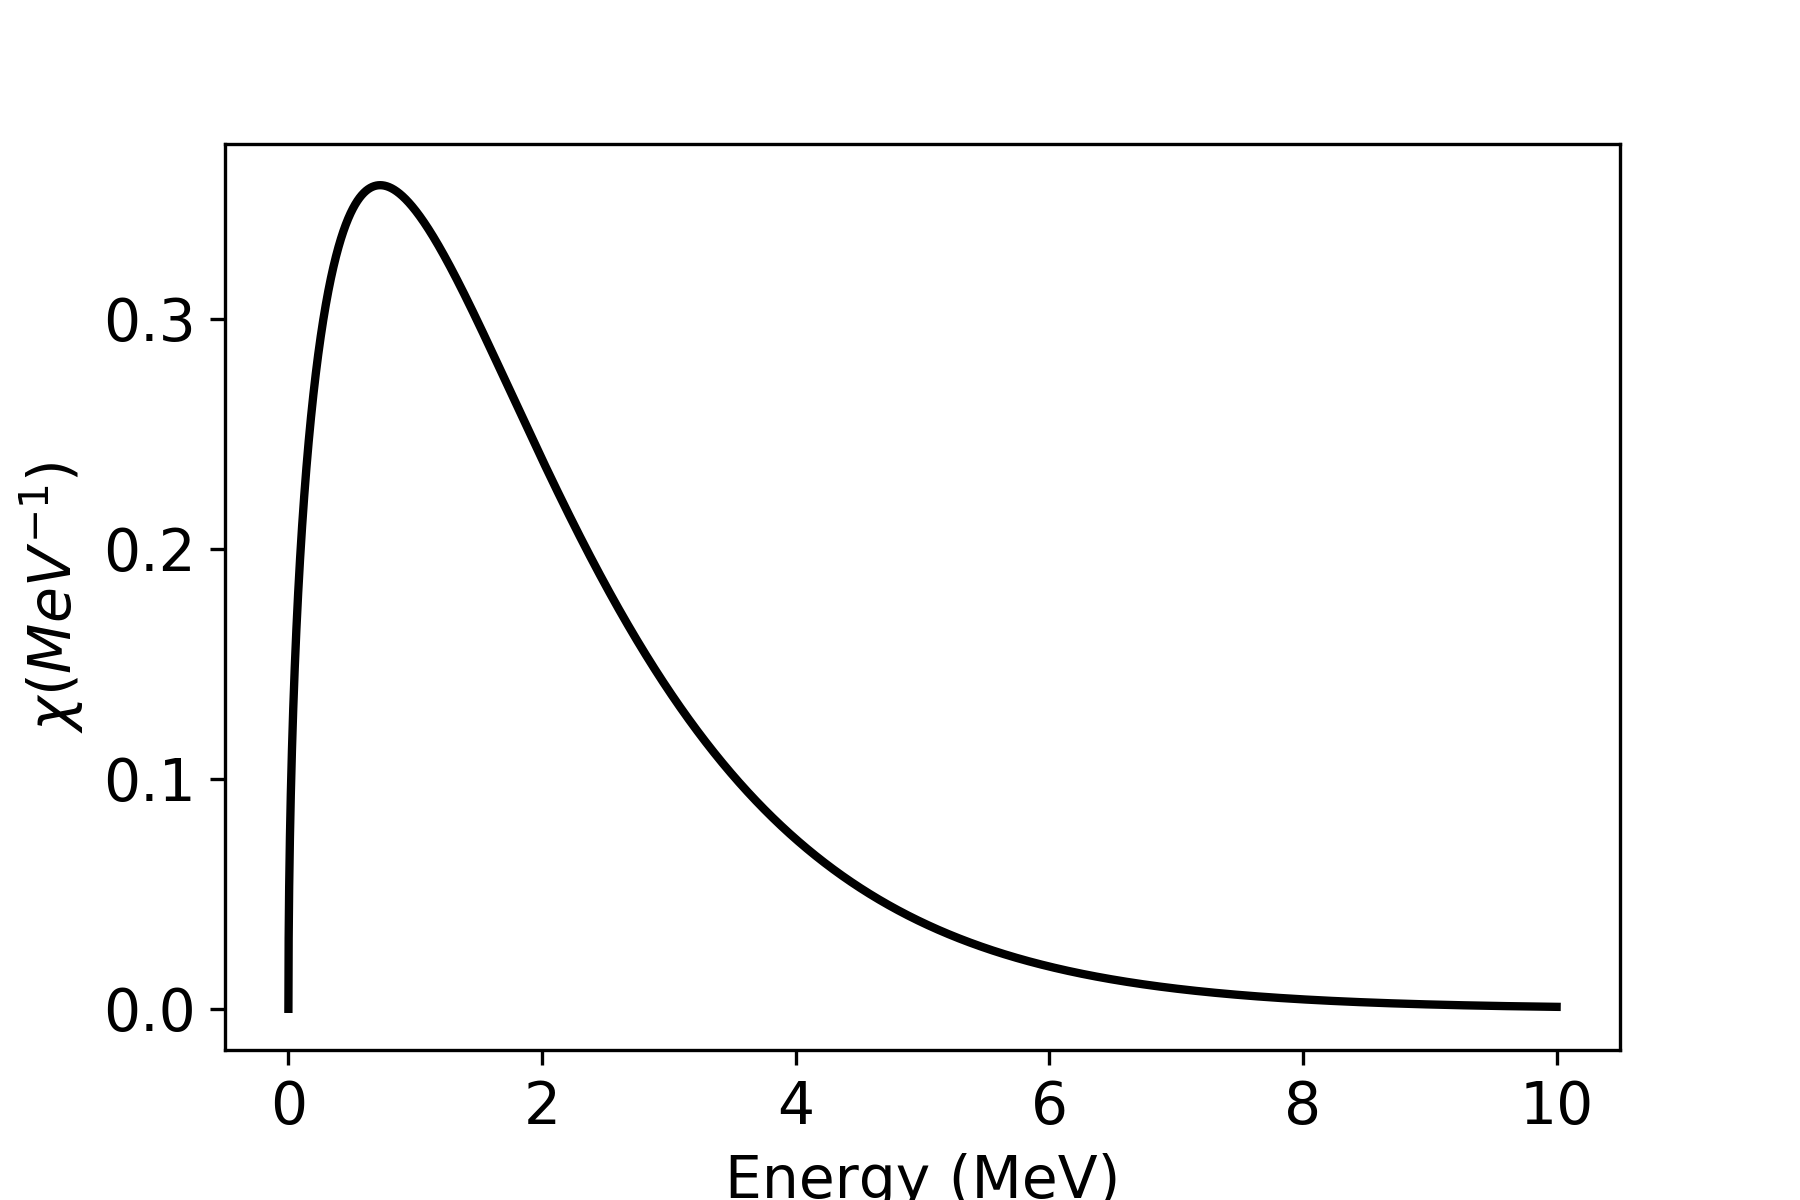
\includegraphics[scale=0.46] {figures/01-watt.png}}\protect
\caption{\label{fig:watt} \footnotesize{Top: The fission birth energy spectrum of neutrons for U235.}}
\end{figure}

\begin{figure}[ht!]
\protect \centering{

\includegraphics[scale=0.46] {figures/01-delayedexample.png}}\protect
\caption{\label{fig:delayedexample} \footnotesize{Example of delayed neutron emission: decay of I-137.}}
\end{figure}

As mentioned earlier some neutrons are emitted with a delay. An example of such delayed neutron emission is shown in Fig. \ref{fig:delayedexample}. I-137 is a fission product with a relatively high fission yield, after $\beta -$ decay it can disintegrate into the metastable state of Xe-137, which then is followed by the emission of a neutron. The time delay is characterized by the half-life of the original $\beta -$ decay (24 sec). We refer to the fission product which decays into the neutron emitting daughter as \textit{delayed neutron precursor}. There are tens of such precursors however in calculations they are usually grouped together into classes with similar half-lifes. Each of these groups can be characterized with

\begin{itemize}
\item $\lambda_i$ the decay constant of the \textit{i}th precursor group
\item $\beta_i$ fraction of all fission neutrons emitted per fission by the \textit{i}th precursor group
\end{itemize} 

The total fraction of delayed neutrons is

\[
\beta=\sum_i \beta_i
\]

and in some textbooks and data sources you can find the average number of delayed neutrons per fission to be given as

\[
\nu_d=\nu\beta
\]


The delayed neutron groups is available for various nuclides, and since the fission yields are different for nuclides, the groups and the total fraction of delayed neutrons are also different. For plutonium isotopes the total fraction is generally lower. As we will see later when discussing transient events in nuclear reactors, the delayed neutrons although contributing with a low fraction have an enormous impact on the time response of the reactor. Delayed neutrons also have a slightly lower energies at birth than prompt neutrons. 

\begin{table}\caption{Delayed neutron fractions of U235}
\centering\begin{tabular}{c | c | c}
Group & $T_{1/2} (s)$ & $\beta_i\cdot 10^5$ \\
\hline
1 & 55.7 & 21 \\
2 & 22.7 & 142 \\
3 & 6.2 & 128 \\
4 & 2.3 & 257 \\
5 & 0.615 & 75 \\
6 & 0.23 & 27 
\end{tabular}
\end{table}

\subsubsection*{Fission fuels: effective number of neutrons}

We have already mentioned that certain nuclides are fissile, while others are fissionable. The only fissile isotope available in nature is U235, which is 0.711 w\% of natural uranium. As we saw will see shortly it is possible to use moderators with low absorption cross section (eg. heavy water) which allow for using natural uranium to build reactor cores, however more often uranium is enriched to contain a larger fraction of U235 than the natural abundance.

\begin{figure}[ht!]
\protect \centering{
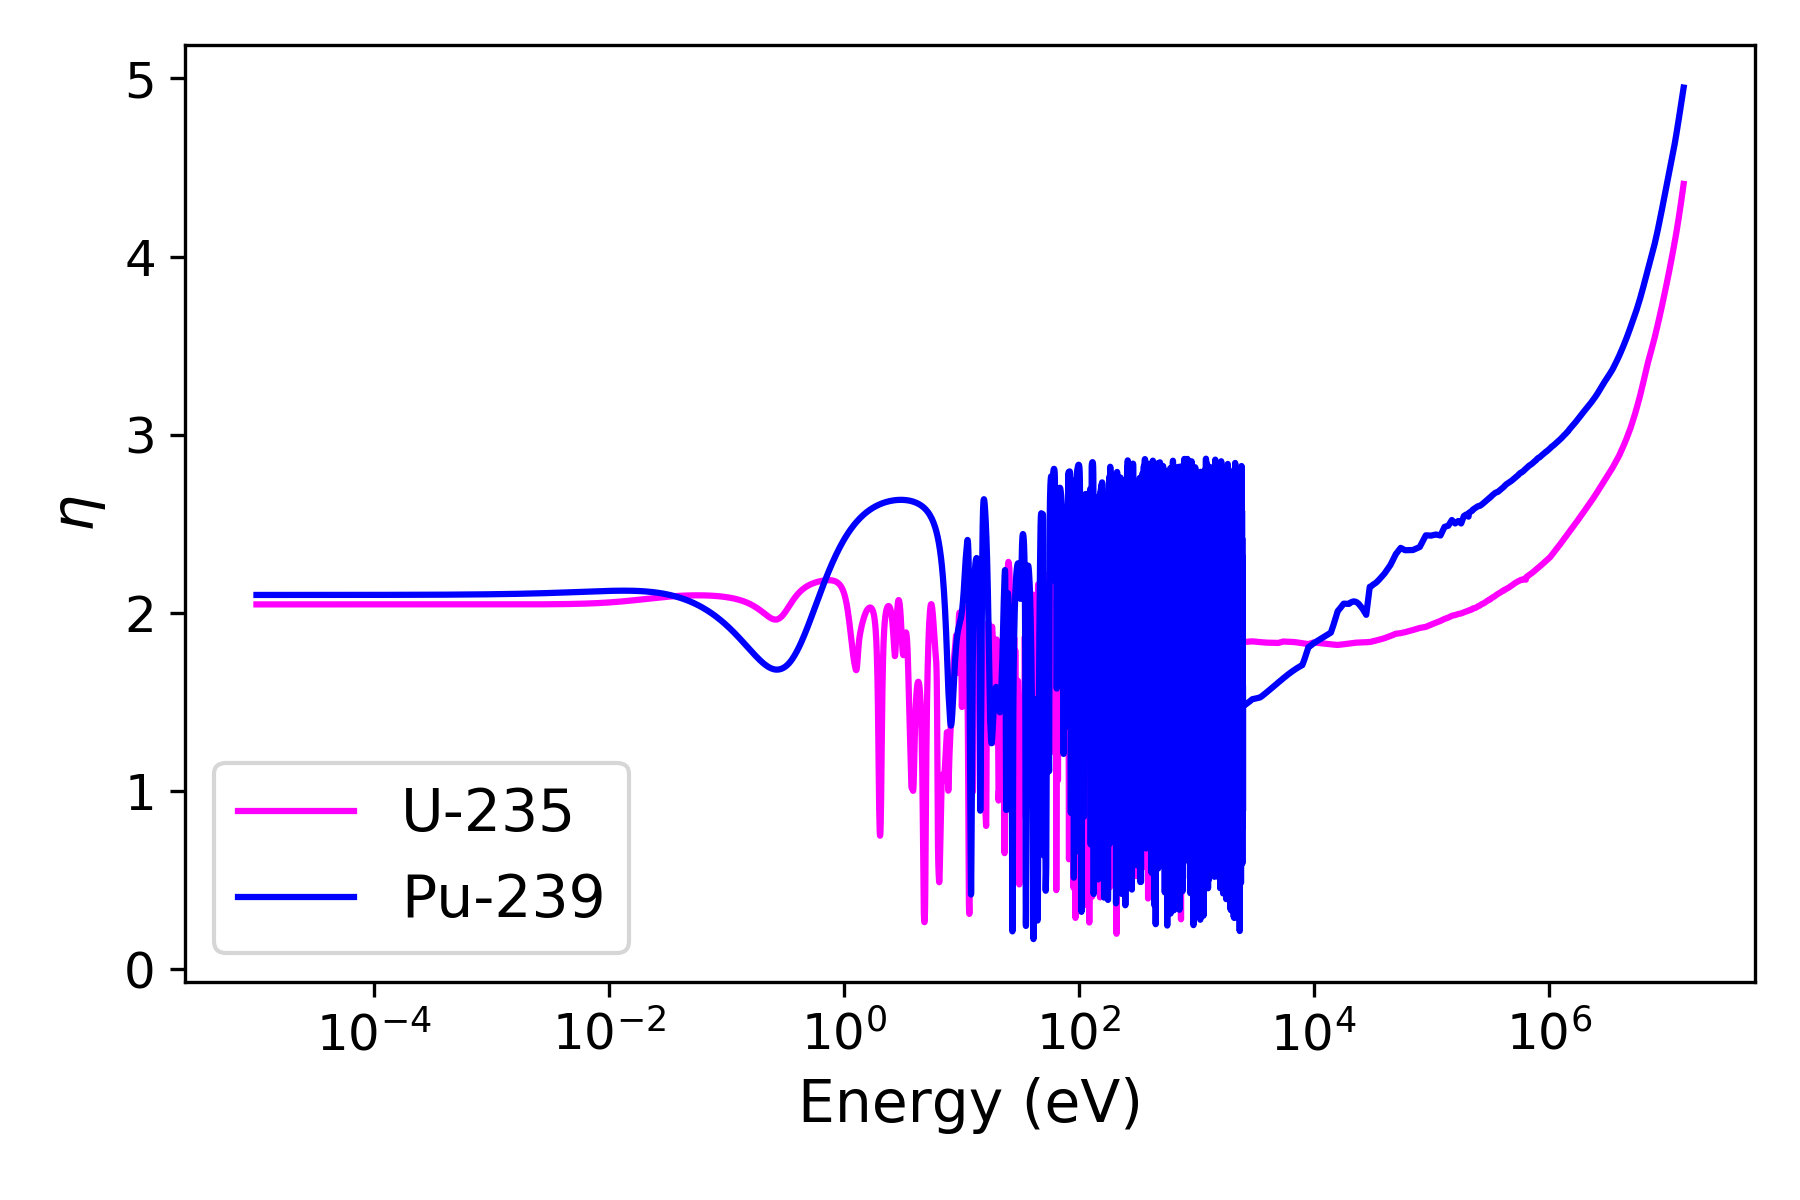
\includegraphics[scale=0.46] {figures/01-PuUeta.png}}\protect
\caption{\label{fig:eta} \footnotesize{Effective number of neutrons for U-235 and Pu-239.}}
\end{figure}

An other possibility is to breed fissile nuclides from fissionable (or due to this reason often called \textit{fertile} nuclides). One such reaction leading to the creation of fissile material in traditional LWR reactors is

\begin{equation}
{}^{238}U\xrightarrow[]{(n,\gamma)}{}^{239}U\xrightarrow[]{\beta^-(23.5m)}{}^{239}Np\xrightarrow[]{\beta^-(2.3d)} {}^{239}Pu
\end{equation}

If one wants to design a reactor which breeds more fissile material than what was initially placed into it (ie. a \textit{breeder} reactor) at least 1 neutron is needed to sustain the chain reaction, and one 1 is needed for breeding (while the rest can be lost due to other parasitic capture reactions. We can define the effective number of neutrons

\begin{equation}
\eta(E)=\nu(E)\frac{\sigma_f(E)}{\sigma_a(E)}
\end{equation}

\noindent which gives the average number of neutrons produced per neutron absorbed in the fuel. If the fuel consists of more nuclides (what is usually the case) we can similarly define

\[
\eta=\frac{\sum_j\nu_j\Sigma_f^j}{\sum_j\Sigma_a^j}
\]

The dependence of this quantity on the neutron energy is shown in Fig. \ref{fig:eta}. We can see that with increasing neutron energy the effective number of neutrons also increases. In order to achieve a self-sustaining chain reaction in a breeder reactor one needs

\begin{equation}
\bar\eta-1-\mathrm{parasitic}-\mathrm{leakage}\geq 1
\end{equation}

\noindent where the loss term is always positive, thus the minimum criterion for break-even breeding $\bar\eta\geq 2$. We can already see that in light water reactors this is very difficult to achieve.




%\end{document}

%\documentclass[12pt]{article}
%\usepackage{amsmath}
%\usepackage{graphicx, color}
%\usepackage{amssymb}
%\usepackage{listings} %source code listing
%\usepackage{multirow}
%%\usepackage[version=2]{mhchem}
%\usepackage{subfig}
%\usepackage{hyperref}
%\usepackage{units}
%\usepackage{gensymb}
%\usepackage{adjustbox}
%\usepackage{listings}
%\usepackage{color}
%\usepackage{tcolorbox}
% 
%\definecolor{codegreen}{rgb}{0,0.6,0}
%\definecolor{codegray}{rgb}{0.5,0.5,0.5}
%\definecolor{codepurple}{rgb}{0.58,0,0.82}
%\definecolor{backcolour}{rgb}{0.95,0.95,0.92}
%
%\newcommand{\specialcell}[2][c]{%
%  \begin{tabular}[#1]{@{}c@{}}#2\end{tabular}}
% 
%
%
%\title{Reactor physics with Python \\ Lecture Notes}
%
%
%\author{Zs.~Elter. E. Branger, M. Preston \\ Uppsala University \\
%        Division of Applied Nuclear Physics}%\corref{cja}}
%%
%\date{2021.}
%\begin{document}

\section{Fission chain reaction and the energy distribution of neutrons}

The requirement to design a self-sustaining nuclear reactor is to achieve a balance in the production and loss of neutrons. This is often referred to as \textit{neutron economy}. As we will see later, the adequate way to study the neutron economy is by developing and solving the neutron transport equation. However, first in this chapter we will define the basic quantities of interest describing fission chain reactions, such as the multiplication factor. Then we will investigate the energy distribution of neutrons in traditional light water reactors and give a rather phenomenological description of the neutron transport process by studying the elements of the \textit{neutron cycle} from the birth of a neutron to its eventual death.


\subsection{Fission chain reaction}

As we discussed earlier the main principle of nuclear reactors that neutrons emerging from fission events are utilized to trigger further fission events, thus giving rise to a chain reaction. If one wants to have a steady chain reaction it needs to be sure that from each fission event on average only 1 neutron is going to cause a following fission event, and the rest of the neutrons are either captured in the reactor materials, or they leak out of the reactor. One common way to describe the fission chain reaction is by defining the \textit{multiplication factor k}:

\begin{equation}\label{eq:kdefault}
k=\frac{\text{Number of neutrons in \textit{i+1}th generation}}{\text{Number of neutrons in \textit{i}th generation}}
\end{equation}

where we define neutron generations: once a neutron triggers fission the new neutrons are considered to be in the next generation. If we follow several neutrons and the same time, and count the number of neutrons they give rise to, we can calculate $k$. Similarly we could have talked about the number of fission events instead. 

The multiplication factor $k$ can be

\begin{itemize}
\item $k<1$: the system is \textit{subcritical} (the number of neutrons decreases from generation to generation, the chain dies out)
\item $k=1$: the system is \textit{critical} (the number of neutrons is the same in each generation and stays always the same)
\item $k>1$: the system is \textit{supercritical} (the number of neutrons increases from generation to generation)
\end{itemize}

When operating the reactor, we usually wish to operate in critical conditions, when the number of neutrons, thus the fission rate, thus the power of the reactor is constant. Nevertheless, the reactor must be able to be supercritical (to increase the power to the required level) and subcritical (to decrease the power or to completely shut down the reactor) as well. Thus one needs to be able to control the reactor.

Nevertheless this often quoted life-cycle point of view definition of the multiplication factor Eq. \ref{eq:kdefault} can be misleading, and is also impractical. The fact is, that it is difficult to follow "one given" generation of neutrons. In fact, in a reactor several "neutron trees" develop at the same time, therefore it is difficult to tag them to decide which generation do they belong too. Also, Fig. \ref{fig:randomtrees} illustrates a simple case: a neutron has probability $p$ to enter fission, and it is lost from the chain otherwise, and in a fission $nu$ neutrons can be generated. A tree with critical conditions might die out, or grow exponentially, and in fact it will be only for the average of several trees that we can obtain the same number of neutrons in the succeeding generations. Of course, in a real nuclear reactor the number of neutrons are very high ($10^9$ neutron/cm$^3$), so we will in fact only see the average behavior. Lastly, what might be misleading here is that the time between the birth and death of a neutron is random (since it depends on the random path distance between collision, and on the number of scattering a neutron enters etc), thus neutrons of the same generation are not aligned so well in time as shown in Fig. \ref{eq:kdefault}. To summarize, care should be taken when thinking of the neutron transport in generations. 

\begin{figure}[ht!]
\protect \centering{
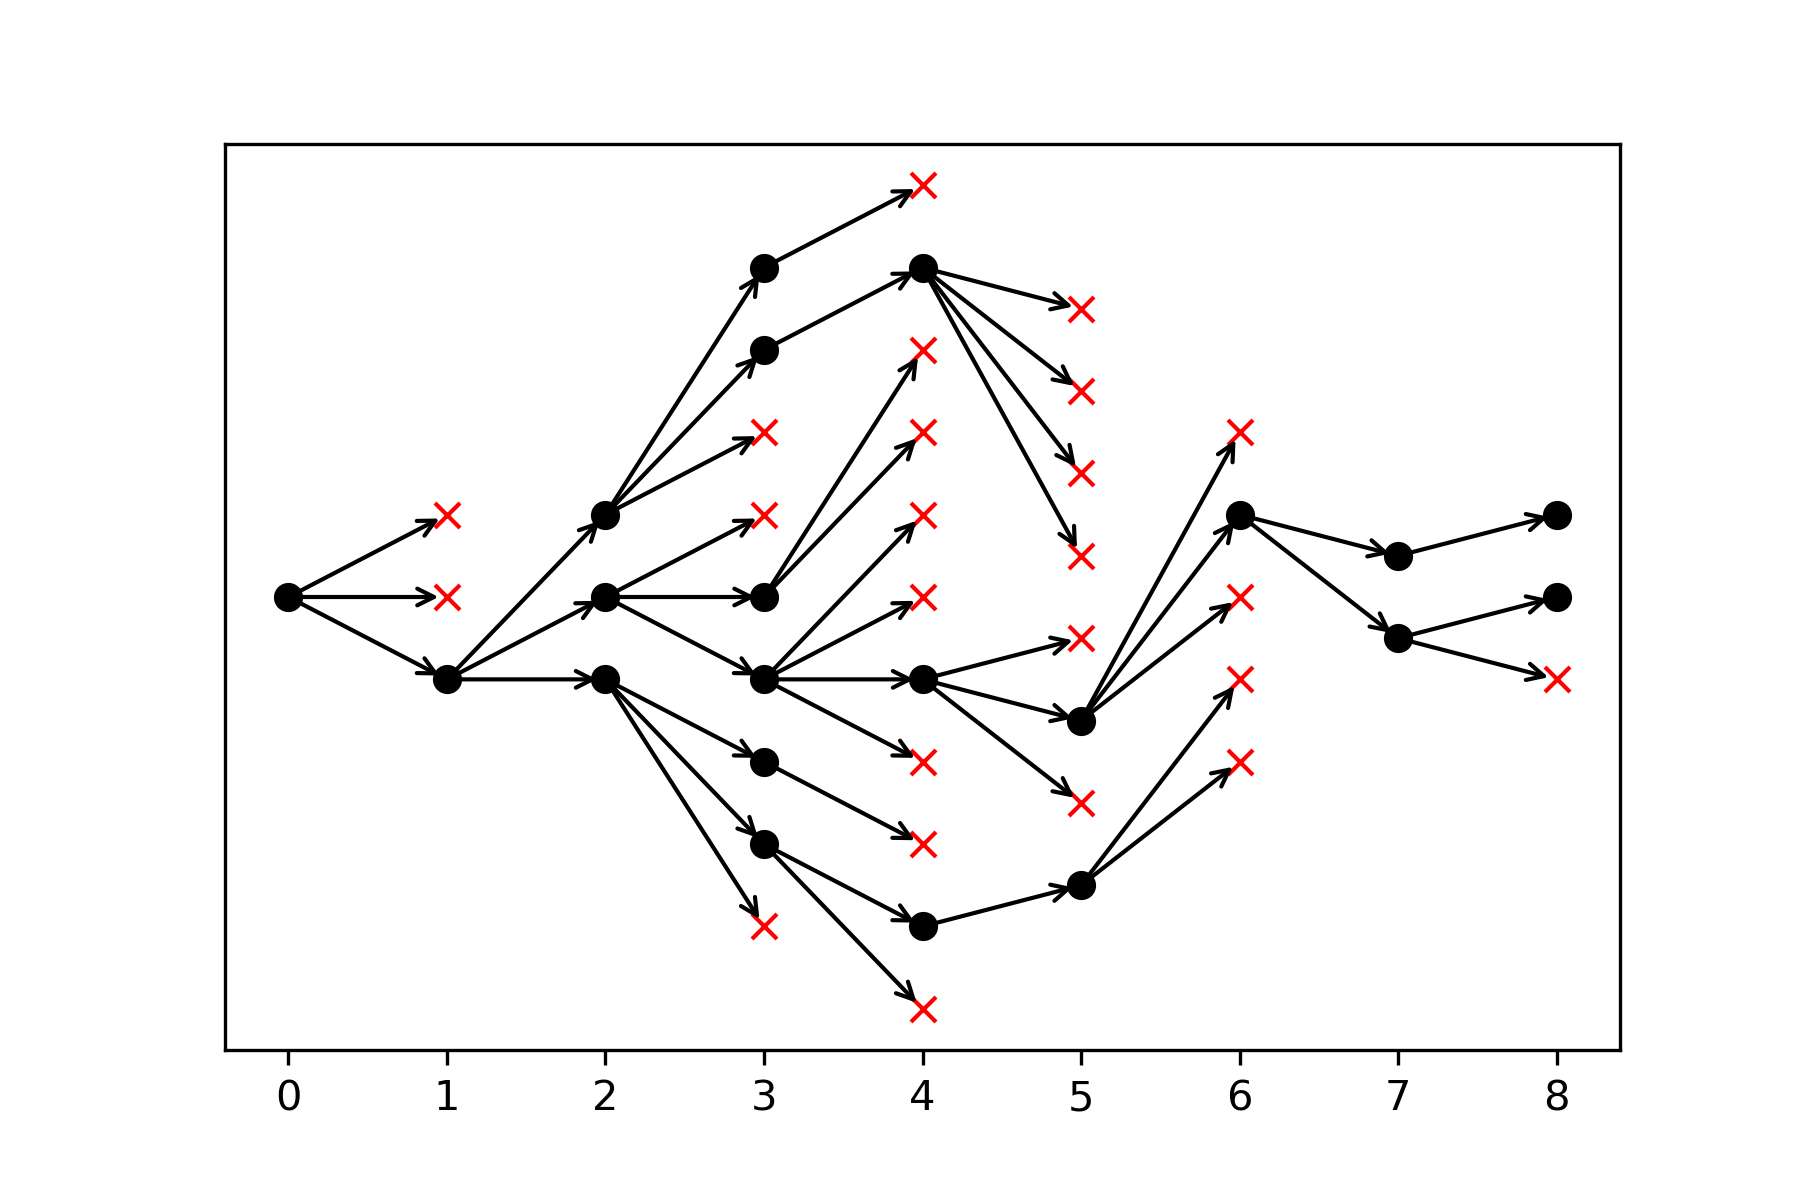
\includegraphics[scale=0.44] {figures/02-randomtreeC.png}
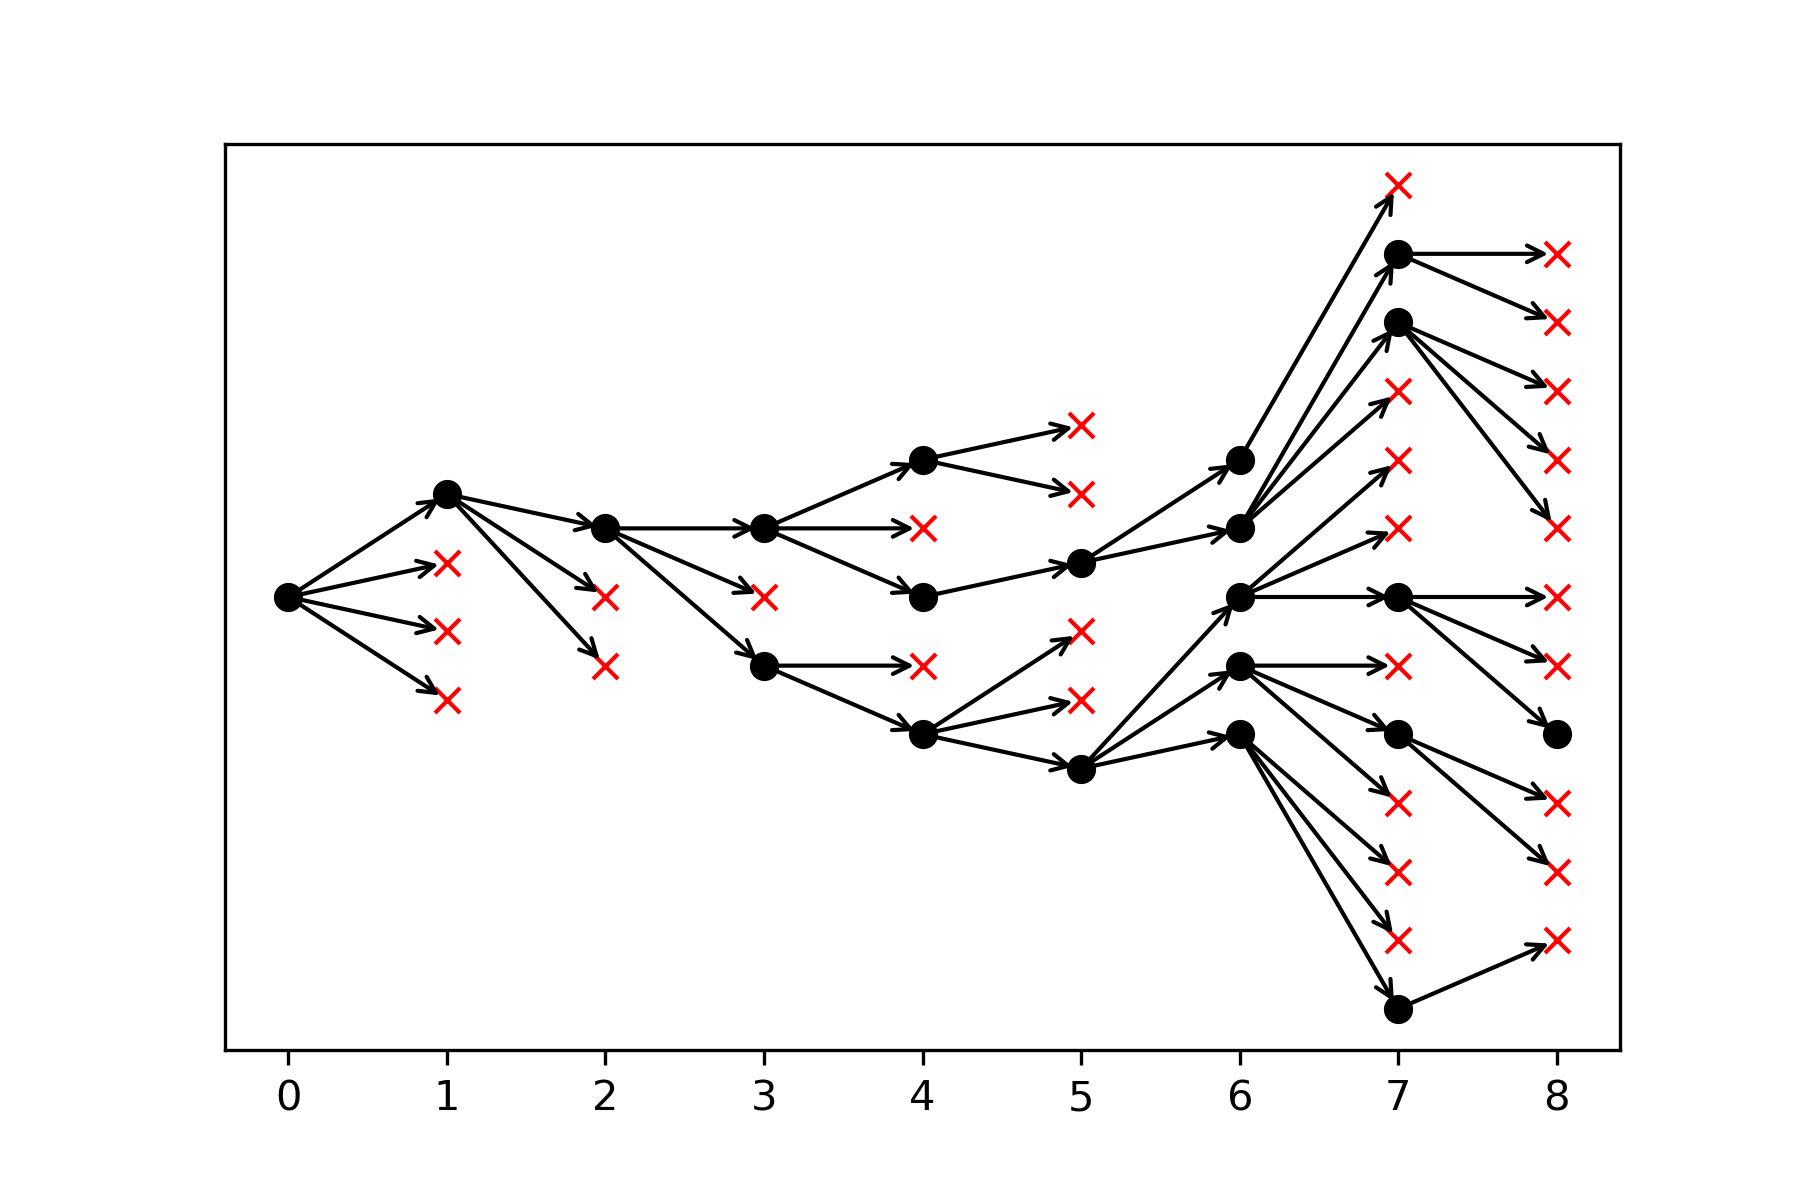
\includegraphics[scale=0.44] {figures/02-randomtreeD.png}
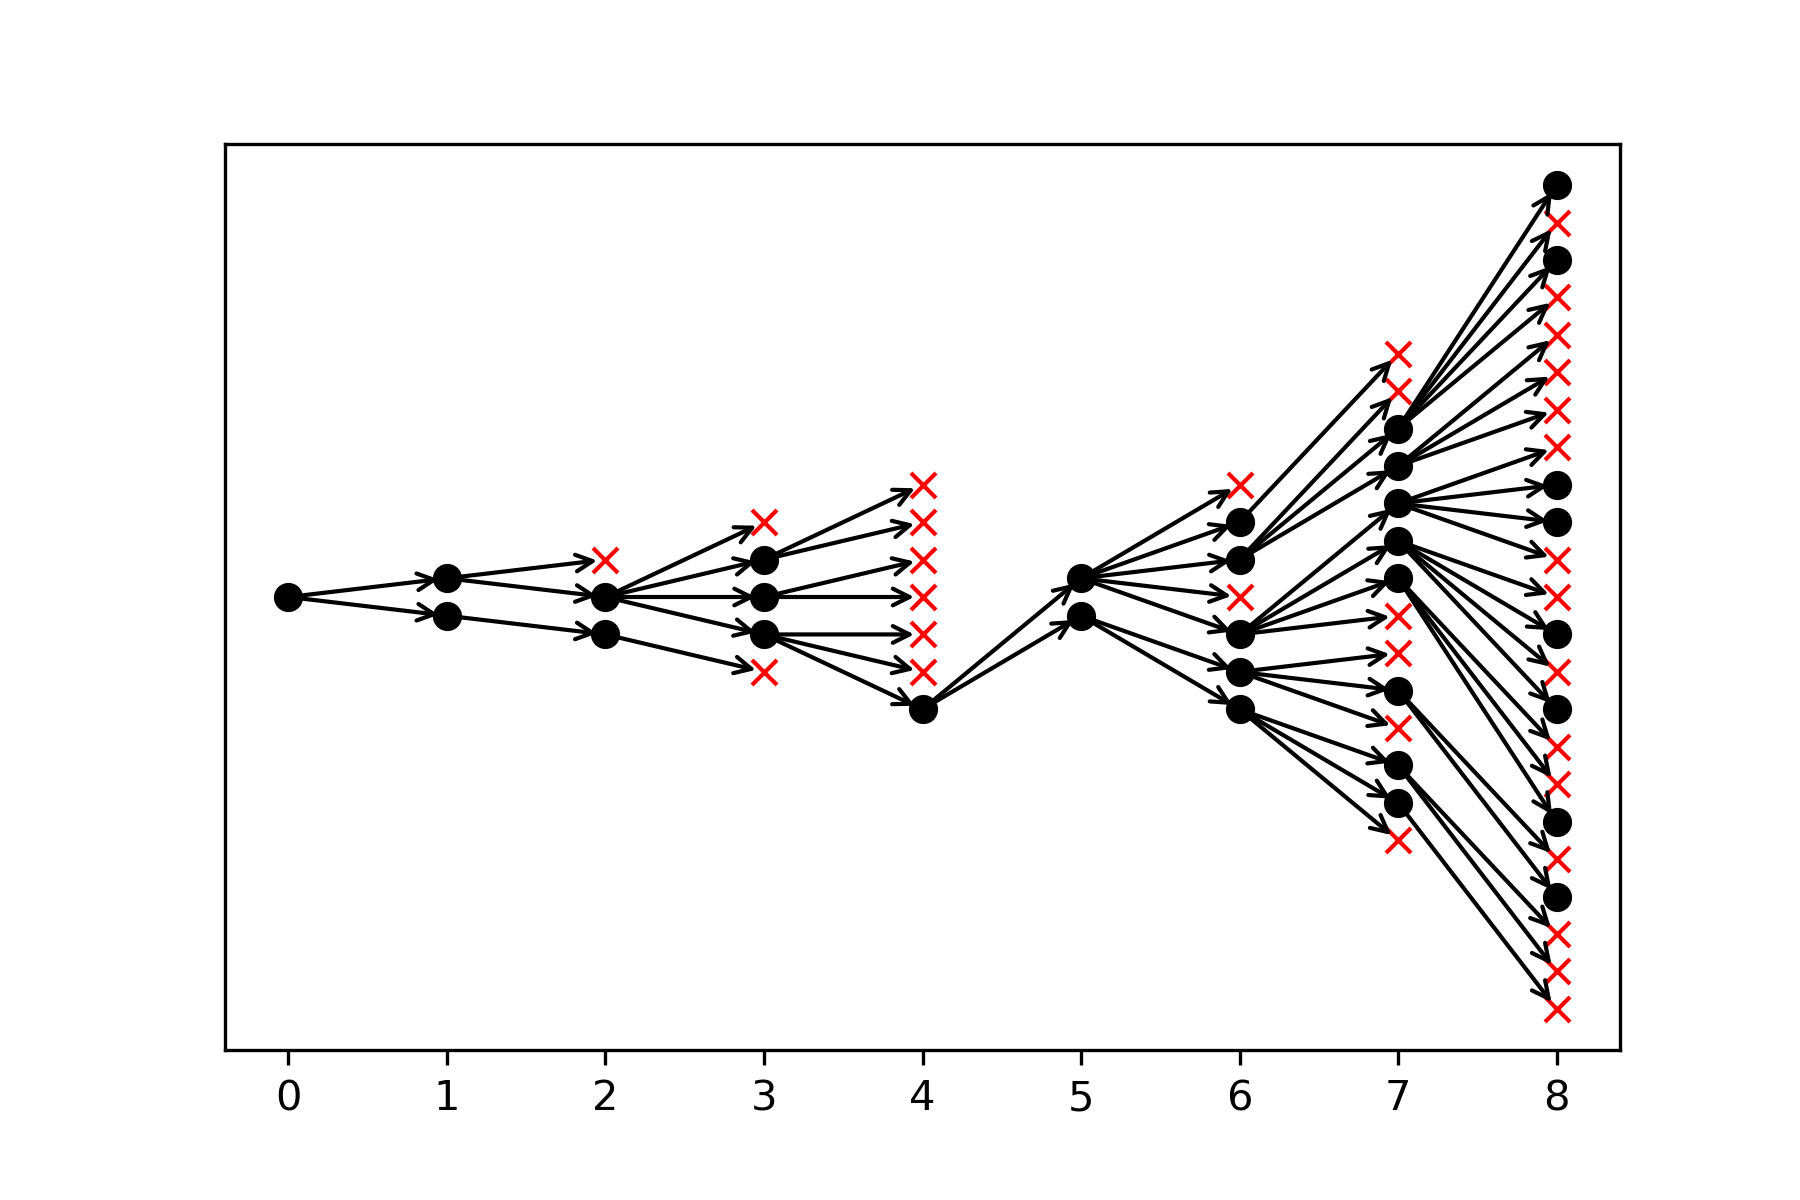
\includegraphics[scale=0.44] {figures/02-randomtreeE.png}
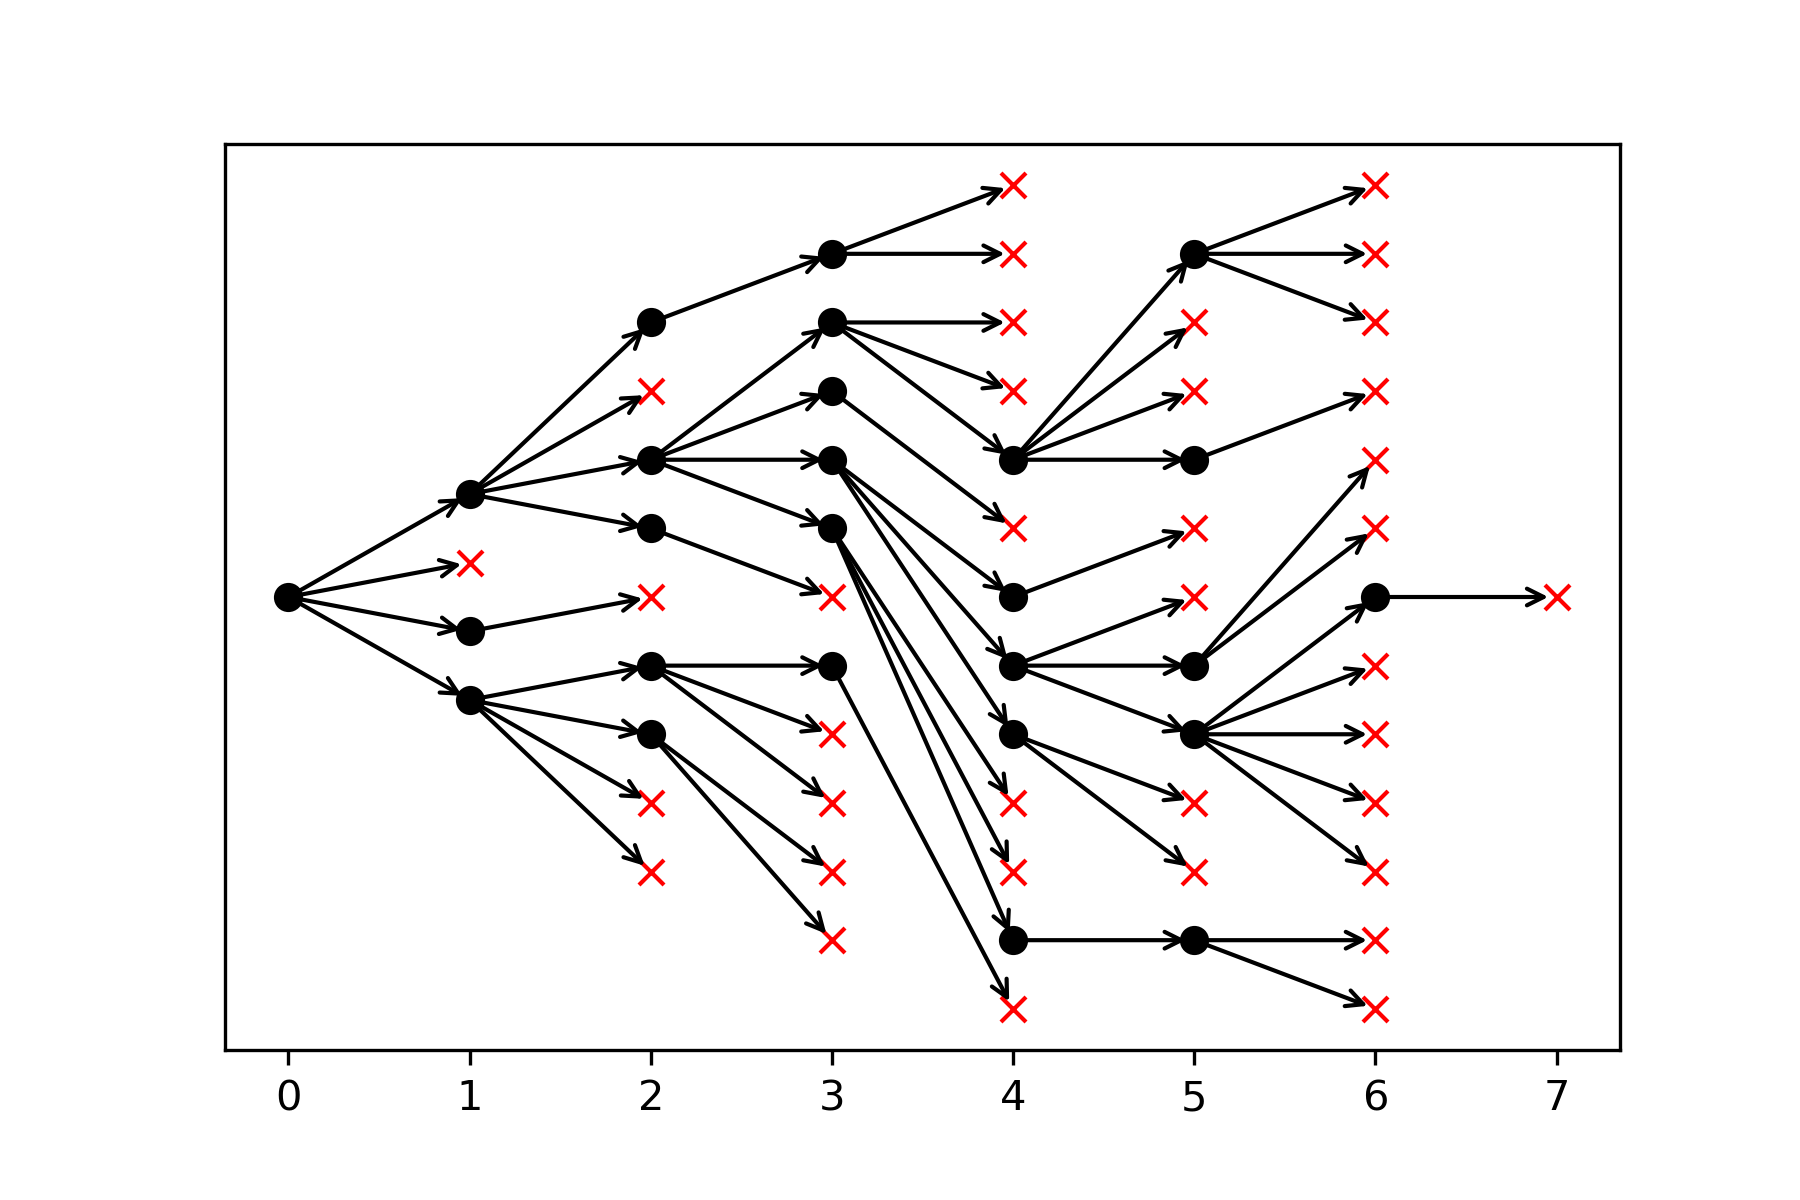
\includegraphics[scale=0.44] {figures/02-randomtreeF.png}}\protect
\caption{\label{fig:randomtrees} \footnotesize{Illustration of random critical trees.}}
\end{figure}

A slightly better and more practical way to define the multiplication factor is through production and loss rates, through the neutron balance (of course such rates also have some fluctuations, so here average rates are meant).

\begin{equation}\label{eq:krates}
k = \frac{\rm {Rate \: of \: neutron \: production}}{\rm Rate \: of \: neutron \: loss \: (absorption \: plus \: leakage) } = \frac{P(t)}{L(t)}
\end{equation}


\noindent where the time can be explicitly considered for the rates (eg. fuel evolution affects production rate, as we will see in later chapters). We will see later, that in fact we will to define the multiplication factor through reaction rates when developing equations to describe neutron transport. We can define the neutron lifetime as

\begin{equation}\label{eq:ell}
\ell=\frac{N(t)}{L(t)}
\end{equation}


\noindent where $N(t)$ is the total neutron population at time $t$. Note that $\ell L(t)$ is the number of lost neutrons during time $\ell$, thus in case $\ell$ is the mean lifetime of neutrons, all neutrons at time $t$ get lost over this time, while of course new neutrons are also generated.

\subsubsection*{Simple kinetics}

If we could somehow measure the exact number of neutrons at time $t$, then the change in $N(t)$ would be

$$\frac{dN}{dt}={\rm Production \: - Loss}=P(t)-L(t)$$

which can be rearranged with \eqref{eq:krates} and \eqref{eq:krates}

\begin{equation}
\frac{dN}{dt}=P(t)-L(t)=\Big(\frac{P(t)}{L(t)}-1 \Big)L(t)=\frac{k-1}{\ell} N(t)
\end{equation}

\noindent This equation we will see later can be derived more rigorously from the neutron diffusion equation. The solution of the equation is simply

\begin{equation}
N(t)=N(0)\exp\Bigg[\Bigg(\frac{k-1}{\ell}\Bigg)t\Bigg]
\end{equation}

\noindent where the value of $k$ will determine the number of neutrons overtime. In Fig. \ref{fig:basickinetics} one can see that for a supercritical system the average number of neutrons increases in time, for a critical system it stays constant and for subcritical system it decreases. This is in agreement with our previous definitions.

\begin{figure}[ht!]
\protect \centering{
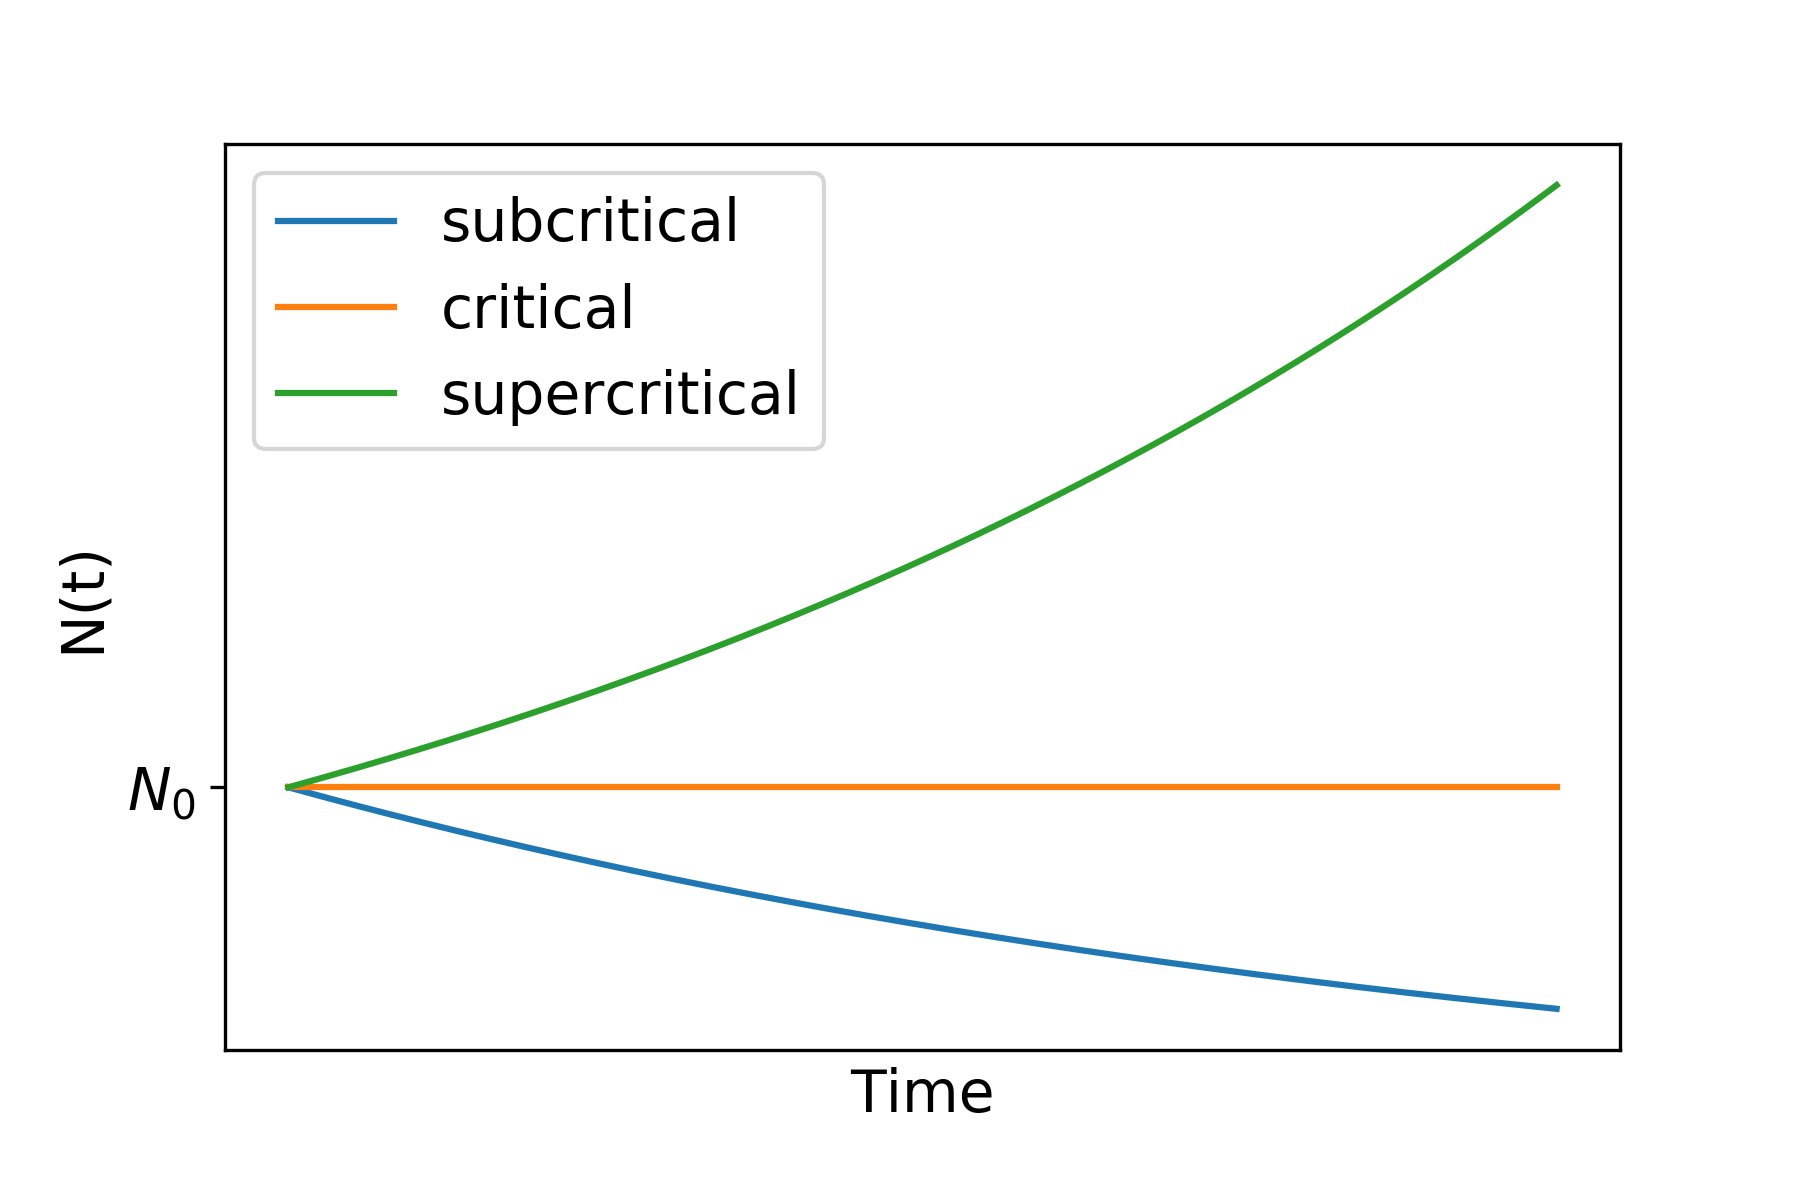
\includegraphics[scale=0.44] {figures/02-basickinetics.png}}\protect
\caption{\label{fig:basickinetics} \footnotesize{Number of neutrons over time.}}
\end{figure}

As a note we can mention here that the average neutron lifetime $\ell$ is around $10^{-4}s$, thus in a slightly supercritical system with $k=1.001$ the number of neutrons would increase by a factor of 22026 in a second. Such a small variation in the multiplication factor is very common in reactors, but such an increase would clearly not be controllable. But as we will see later, the presence of delayed neutrons does significantly increase the average lifetime of neutrons, and it makes the time behavior of reactors manageable.

\subsubsection*{2 factor formula}

Let us make a thought experiment in order to study the k-effective. Consider a homogeneous mixture of some nuclear fuel (uranium) and other cooling and structural materials. For our neutron trees in Figure \ref{fig:randomtrees} we considered that the neutron branch either dies out or initiates a fission event producing other neutrons. There are more way to die (or become irrelevant for the chain reaction) for a neutron. As illustrated in Figure \ref{fig:2factors}, there in fact, in a finite core the neutron either gets absorbed or leaves the system before interacting with it. Let's consider that the probability of non-leakage is $P_{NL}$. Then the neutron can be absorbed by a fuel nucleus or by some other nucleus (this is called \textit{parasitic capture}. Let's denote the conditional probability of the neutron being absorbed in fuel if it is absorbed with $P_{AF}$. Finally, the conditional probability if the neutron is absorbed in the fuel then it will initiate a fission event is $P_f$. After fission a number ($\nu$) of neutrons emerge.

\begin{figure}[ht!]
\protect \centering{

\includegraphics[scale=0.44] {figures/02-2factor.png}}\protect
\caption{\label{fig:2factors} \footnotesize{Probabilistic approach of understanding the multiplication factor.}}
\end{figure}

If $N_i$ neutrons started in a given generation, then it is easy to see that in the next generation the number of neutrons will be

$$N_{i+1}=\nu P_{NL}P_{AF}P_{f}N_i$$

therefore

$$k=\frac{N_{i+1}}{N_i}=\nu P_{NL}P_{AF}P_{f}$$

In order to assign actual physical quantities to these probabilities we have to remind ourselves that the cross sections of neutron-nucleus interactions characterized the probability of the event occurring. With little reasoning we can see that

$$f\equiv P_{AF} = \frac{\Sigma_a^F}{\Sigma_a}$$

\noindent where we introduced a new notation commonly used in the literature for the \textit{thermal utilization}. Similarly 

$$\eta \equiv \nu P_f= \nu\frac{\Sigma_f^F}{\Sigma_a^F}$$

\noindent where we found a quantity we have already looked upon, the \textit{thermal fission factor} or reproduction factor.

The non-leakage probability is more difficult to obtain, since it depends on the geometry of the core. Nevertheless, since $f$ and $\eta$ depend on the material properties only, often the infinite multiplication factor 

$$k_\infty=\eta f$$

is introduced to describe the multiplication of an infinite system (where neutrons cannot leak out). 

This simple model however does not account for the fact that in a thermal reactor the neutrons can have a wide range of energies, since they are born with energies in the order of MeV, however the fission reactions happen in the order of eV. Also, neutron cross sections have a strong dependence from the energy, as we saw earlier often with sudden jumps in the cross section. In order to refine our simple \textit{2 factor} model we will need to study the spectrum of neutrons.

\subsection{Neutron spectrum: Slowing down and thermalization}

With our previous studies we already have the intuition that neutrons can travel at very different speed in the reactor. They are born with relatively high (order of magnitude MeV) energies from fission, then they loose their energy in scattering reactions until they reach the thermal energies, when they can even gain energy from the nuclei of the medium. The energy distribution of the neutrons is called \textit{neutron spectrum}, and is defined as 

$$\Phi(E)=v(E)n(E) \: \Big[\frac{\text{n}}{\text{cm}^2\cdot\text{s}\cdot\text{eV}}\Big]$$

\noindent where $v(E)$ is the speed of neutrons and $n(E)dE$ is the number of neutrons in the energy interval $[E,E+dE]$. The main goal of this section is to determine $\Phi(E)$.

We can also recall that we have previously defined the reaction rate, and similarly we can define the spectral reaction rate quantities, eg. for some reaction$i$

$$R_i(E)=\Sigma_i(E)\Phi(E)$$

thus the total reaction rate is

$$R_i=\int_0^\infty\Sigma_i(E)\Phi(E)dE$$

In this section we will try to make a rough, quantitative analysis of the spectrum with the intention of introducing physical quantities relevant for the discussion of neutron slowing down and our goal will be to sketch the shape of the energy distribution. However we will neglect several aspects, for example space-dependent slowing down, and assume that the slowing down takes place in an infinite medium without spatial dependence.

Besides our curiosity, there is an other practical reason to calculate the neutron spectrum in a reactor: as we will see later, for the numerical treatment of neutron transport it is not possible to use the cross sections in their continuous form, instead we have to calculate weighted averages of the cross section, where the weighting function is going to be the spectrum. 

The difficulties to estimate the neutron spectrum arise from the fact that at various energies the phenomena at play to govern the transport of neutrons is different. Commonly, we separate three energy regions, which can be characterized with the following phenomena:

\begin{itemize}
\item Thermalization (0-1 eV): Upscattering due to thermal motion; Chemical binding and crystalline effects.
\item Slowing down or moderation (1-$10^5$eV): Elastic scattering from free nuclei at rest, isotropic in CM; Resolved resonances
\item Fast fission: Elastic scattering anisotropic in CM; inelastic scattering; Unresolved resonances
\end{itemize}

First we will introduce moderation (the slowing down of neutrons) in a rather heuristic way, and then we will study the spectrum at different energies.

\subsubsection{Moderation and moderators}

We can recall from the study of elastic scattering that the ratio of the neutron energy before ($E_i)$ and after scattering ($E_f$) is constant for a given CM scattering angle $\theta_C$:

\begin{equation}\label{eq:muErelation2}
\frac{E_f}{E_i}=\frac{(1+\alpha)+(1-\alpha)\cos\theta_C}{2}
\end{equation}

\noindent where $\alpha=(A-1)^2/(A+1)^2$, which means that the change of the logarithm of the energy is constant. We can define the average logarithmic decrement

\begin{equation}
\xi = \int\limits_0^{E_i}\ln\Big(\frac{E_i}{E_f}\Big)P(E_i\rightarrow E_f)dE_f=1+\frac{\alpha}{1-\alpha}\log\alpha \approx \frac{2}{A+2/3}
\end{equation}

\noindent where we introduced the scattering kernel from our previous studies, and the last approximation holds for not too small $A$.

In case of a homogeneous mixture of nuclides we can weight with the scattering cross section:

$$\bar\xi = \frac{\sum_i\xi_i\Sigma_{si}}{\sum_i\Sigma_{si}}$$

The value of $\xi$ characterizes how many scattering reactions are needed to slow down the neutrons. The larger the value of $\xi$ the less scattering is needed. Materials which is can efficiently slow down neutrons we call \textit{moderators}. The average number of collisions to slow a neutron from fast energies to thermal energies can be calculated with

$$\frac{1}{\xi}\ln(2 MeV/0.025 eV)=\frac{18.2}{\xi}$$

The ability of slowing down neutrons can be characterized with \textit{moderating power} $\xi\Sigma_s$: the logarithmic energy loss per distance traveled by the neutron. However, when assessing how good a moderator is, we have to consider also how much neutrons are absorbed by the moderator, therefore we can define the \textit{moderating ratio}

$$\xi\Sigma_s/\Sigma_a$$

\noindent As we see from Table \ref{tab:moderator}, the best moderators the ones containing low mass nuclei. However we can also notice, that even though hydrogen is the lightest, it is not the best moderator, when considering absorption as well. This is the reason that for a reactor moderated with light water one needs to enrich uranium in order to make it critical. However if a reactor is moderated with heavy water (such as the CANDU reactors) or graphite (such as the MAGNOX reactors), criticality can be achieved with natural uranium as well. There is obviously a compromise whether we spend our efforts on enriching the fuel, or producing heavy water. 


\begin{table}\caption{Moderating properties of various materials}\label{tab:moderator}
\begin{tabular}{c | c | c | c | c | c | c}
Moderator & $A$ & $\alpha$ & $\xi$ & $18.2/\xi$ & $\xi\Sigma_s (\text{cm}^{-1})$ & $\xi\Sigma_s/\Sigma_a$ \\
\hline
H & 1 & 0 & 1.0 & 18 & 1.3 & 61 \\
D & 2 & 0.111 & 0.725 & 25 & 0.08 & 2538 \\
Be-9 & 9 & 0.64 & 0.2 & 87 & 0.15 & 125 \\
C-12 & 12 & 0.716 & 0.158 & 115 & 0.061 & 190 \\
U-238 & 238 & 0.983 & 0.0084 & 2172 & 0.04 & 0.16
\end{tabular}
\end{table}

\subsubsection*{Lethargy}

When discussing slowing down it is often more natural to use an other variable than energy, the \textit{lethargy}, which often feels intimidating for novice reactor physicist. Although we promise we will not overuse it in this course, but since the reader will find this variable in other books, it is necessary to introduce it. The lethargy gives the logarithmic energy loss compared to some fix energy $E_0$:

$$u=\ln(E_0/E)$$

$$E=E_0\exp(-u)$$

\noindent where $E_0$ is typically the energy of the source or a sufficiently high energy (eg. 10 MeV) in case of fission sources). We can notice  that $\xi$ is the average increase of lethargy in a collision. The neutron flux therefore can be written as

$$\Phi (u)du=\Phi (u)dE/E=\Phi (E)dE$$

$$\Phi(u)=\Phi(E)E$$

Figure \ref{fig:lethargy} makes it even more apparent why working with the lethargy is more natural in slowing down. We can see that the collision density (as discussed soon) is constant. We can also notice that the lethargy is increasing during slowing down: as neutrons get slower they get more "lethargic".

\begin{figure}[ht!]
\protect \centering{
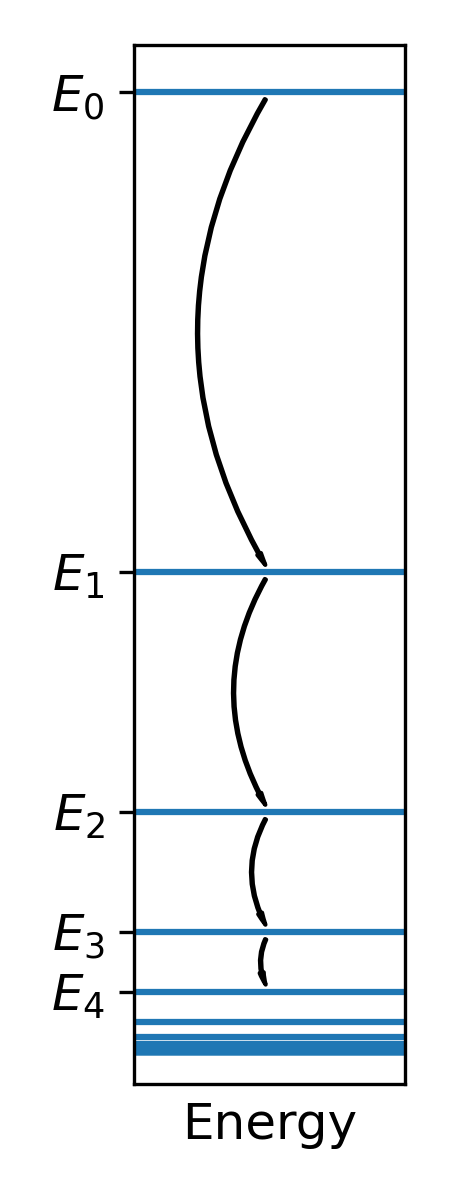
\includegraphics[scale=0.74] {figures/03-energychange.png}
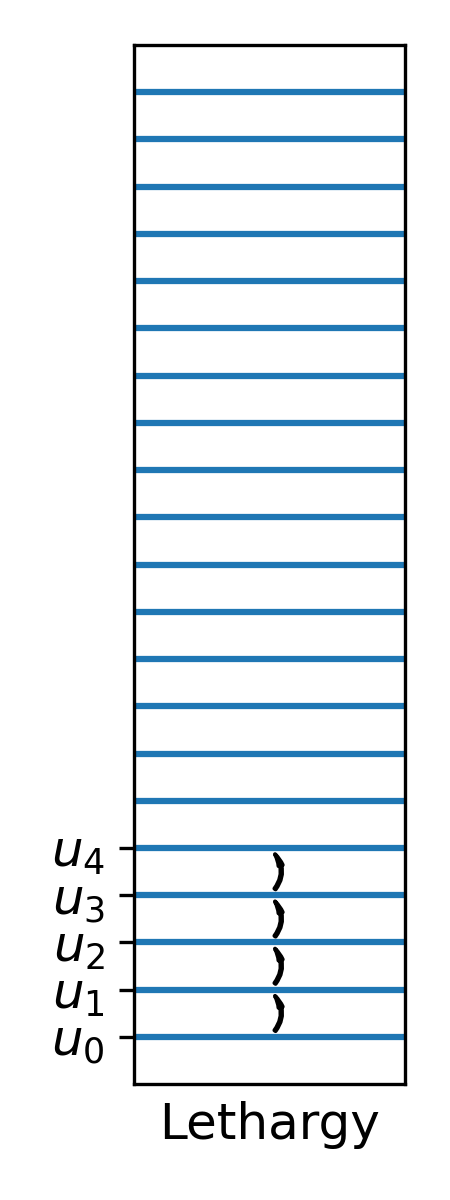
\includegraphics[scale=0.74] {figures/03-lethargychange.png}}\protect
\caption{\label{fig:lethargy} \footnotesize{Schematic illustration of energy and lethargy change during slowing down.}}
\end{figure}

\subsubsection{Neutron spectrum}

We will discuss the neutron spectrum in the three regions (thermal, moderate, fast) separately.

\subsubsection*{Fast and thermal region}

For the fast region we consider that the source of neutrons are the fission events, and little reactions happen to them, therefore the spectrum in this region can be well approximated with the Watt-spectrum. As we will see later in more realistic Monte Carlo calculation, although the shape indeed resembles the fission birth spectrum, but it is not entirely smooth.

For thermal energies, where neutrons can both loose or gain energy in scattering events, we can assume that the neutron spectrum follows the Maxwell-distribution

$$\phi(E)\propto E\exp\big(-\frac{E}{kT}\big)$$

\noindent although it has to be mentioned that in reality due to absorbing events taking place at these energies, the real neutron spectrum is slightly shifted to higher energies, this is called spectral hardening.

\subsubsection*{Slowing down region}

We will consider the slowing down in an infinite, homogeneous geometry and assume that the neutron source is spatially uniform. First, we will develop an equation describing the slowing down.

Let us notice that 

\begin{itemize}
\item $\Sigma_t(E)\Phi(E)dE$ is the number of collisions per unit time within $[E,E+dE]$ which removes neutrons from the energy interval.
\item $S(E)dE$ is the number of neutrons emitted per unit time within $[E,E+dE]$
\item $\int\limits_0^\infty \Phi(E')\Sigma(E'\rightarrow E)dE'dE$ is the number of neutrons per unit time reaching $[E,E+dE]$ through scattering
\end{itemize}

In case of steady state, we can assume that the source terms (the source and the in-scattering events) are in balance with the loss term (the total number of collisions removing neutrons from our energy interval):

\begin{equation}
\int\limits_0^\infty \Phi(E')\Sigma(E'\rightarrow E)dE'+S(E)=\Sigma_t(E)\Phi(E)
\end{equation}

\noindent is the \textit{slowing down equation} which as we will see in the next chapter could be derived directly from the general neutron transport equation.

Let us consider that inelastic scattering can be neglected for energies below 100 keV and elastic scattering can be considered isotropic in CM, and recall the scattering kernel for elastic scattering:\footnote{Note, that previously we used the $(E\rightarrow E')$ notation, since we were curious which energies are reached from our initial energy $E$, now we swapped the notation of initial and final energy, because we are more interested in which energies contribute to our final energy, and it is more convenient to develop the equation for variable $E$. Nevertheless the meaning is still the same: $E_{initial}\rightarrow E_{final}$}

\begin{equation}\label{eq:scatkernel}
    \Sigma_s(E'\rightarrow E) = 
    \begin{cases}
      \frac{\Sigma_s(E')}{(1-\alpha)E'} & \text{if} \: \alpha E' \leq E \leq E' \\
      0 & \text{otherwise}
    \end{cases}
\end{equation}

\noindent In case of a mixture of various nuclides the scattering kernel would be the sum of the scattering kernels of each nuclide. However, in practice usually there is one type of nuclide which has much better moderating properties than the others, thus we can neglect the contribution of the others. By substituting this kernel into the slowing down equation we arrive to

\begin{equation}\label{eq:slowingdown}
\int\limits_E^{E/\alpha} \Phi(E')\frac{\Sigma_s(E')}{(1-\alpha)E'}dE'+S(E)=\Sigma_t(E)\Phi(E)
\end{equation}

\noindent which looks fairly innocent, but in practice can be easily tackled only in a couple of situations:

\begin{enumerate}
\item Slowing down without absorption ($\Sigma_a=0 \rightarrow \Sigma_t=\Sigma_s$)
\item Slowing down on hydrogen nuclei with absorption
\item Slowing down on arbitrary nuclide but with energy independent cross sections
\end{enumerate}

Of course in practice the most important case would be to solve the equation for arbitrary nuclides and energy dependent cross sections, however for that case no analytic solution is available. In this lecture note we are going to discuss 1. and 2., since they will provide enough insight about the neutron spectrum in this region.

\vspace{0.5cm}

\textbf{Slowing down without absorber}

As we noticed earlier the energy lost during scattering is decreasing during slowing down, however the average increase of lethargy is independent of the lethargy. Thus the number of collisions per time and unit energy in the energy bin $[E,E+dE]$, the collision density $F(E)=\Sigma_t(E)\Phi(E)$ is increasing with decreasing $E$. However the number of collisions per unit time per unit lethargy is independent of $u$. Thus

$$F(u)=\Sigma_t(u)\Phi(u)=\Sigma_t(E)\Phi(E)E=c$$

\noindent if we substitute $\Sigma_t(E)\Phi(E)=c/E$ in Eq. \eqref{eq:slowingdown}, we will find that indeed it is a solution if $\Sigma_t=\Sigma_s$ and at energies below the energies of the source (ie. when S(E)=0).

We can obtain $c$ by noticing that the number of neutrons per unit time whose energy passes above a given lethargy is the same as the number of neutrons emitted per unit time since there is no absorption. The number of neutrons emitted per unit time is simply the integral of the source neutron spectrum.

$$S=\int\limits_{E_S}^\infty S(E)dE$$

\noindent where $E_S$ is the energy below which the source does not emit neutrons. 

And the number of neutrons passing lethargy $u$ per unit time is $c\xi$, since all the neutrons will pass lethargy $u$ which suffered a collision between $u$ and $u-\xi$, therefore we can conclude that\footnote{Notice that $c=F(u)$, the collision density. The collision density is defined so that $F(u)du$ gives the number of collisions within [u,u+du] therefore $\int\limits_{u-\xi}^u F(u)du$ is the number of neutrons passing lethargy $u$. Therefore $S=F(u)\xi=c\xi$ }

$$c\xi=S$$

$$\Phi(E)=\frac{S}{\xi E\Sigma_s(E)}=\frac{S}{\xi E\Sigma_t(E)}$$

\noindent therefore if we combine our comments on the thermal and fast regions with our recent findings, we can illustrated our idealized neutron spectrum in Figure \ref{fig:idealneutronspectrum}. Notice that we have plotted both $\Phi(E)$ and the lethargic spectrum $E\Phi(E)$. As we will see later, indeed this rough sketch explains the main features of our actual neutron spectra in thermal systems rather well.

It also needs to be highlighted again, that these results are valid only at energy regions below the source energy. This is often called \textit{asymptotic region}. It is also important to point out that the scattering cross section can be considered independent of energy in the slowing down region, therefore $\Phi(E)\propto 1/E$.

\begin{figure}[ht!]
\protect \centering{
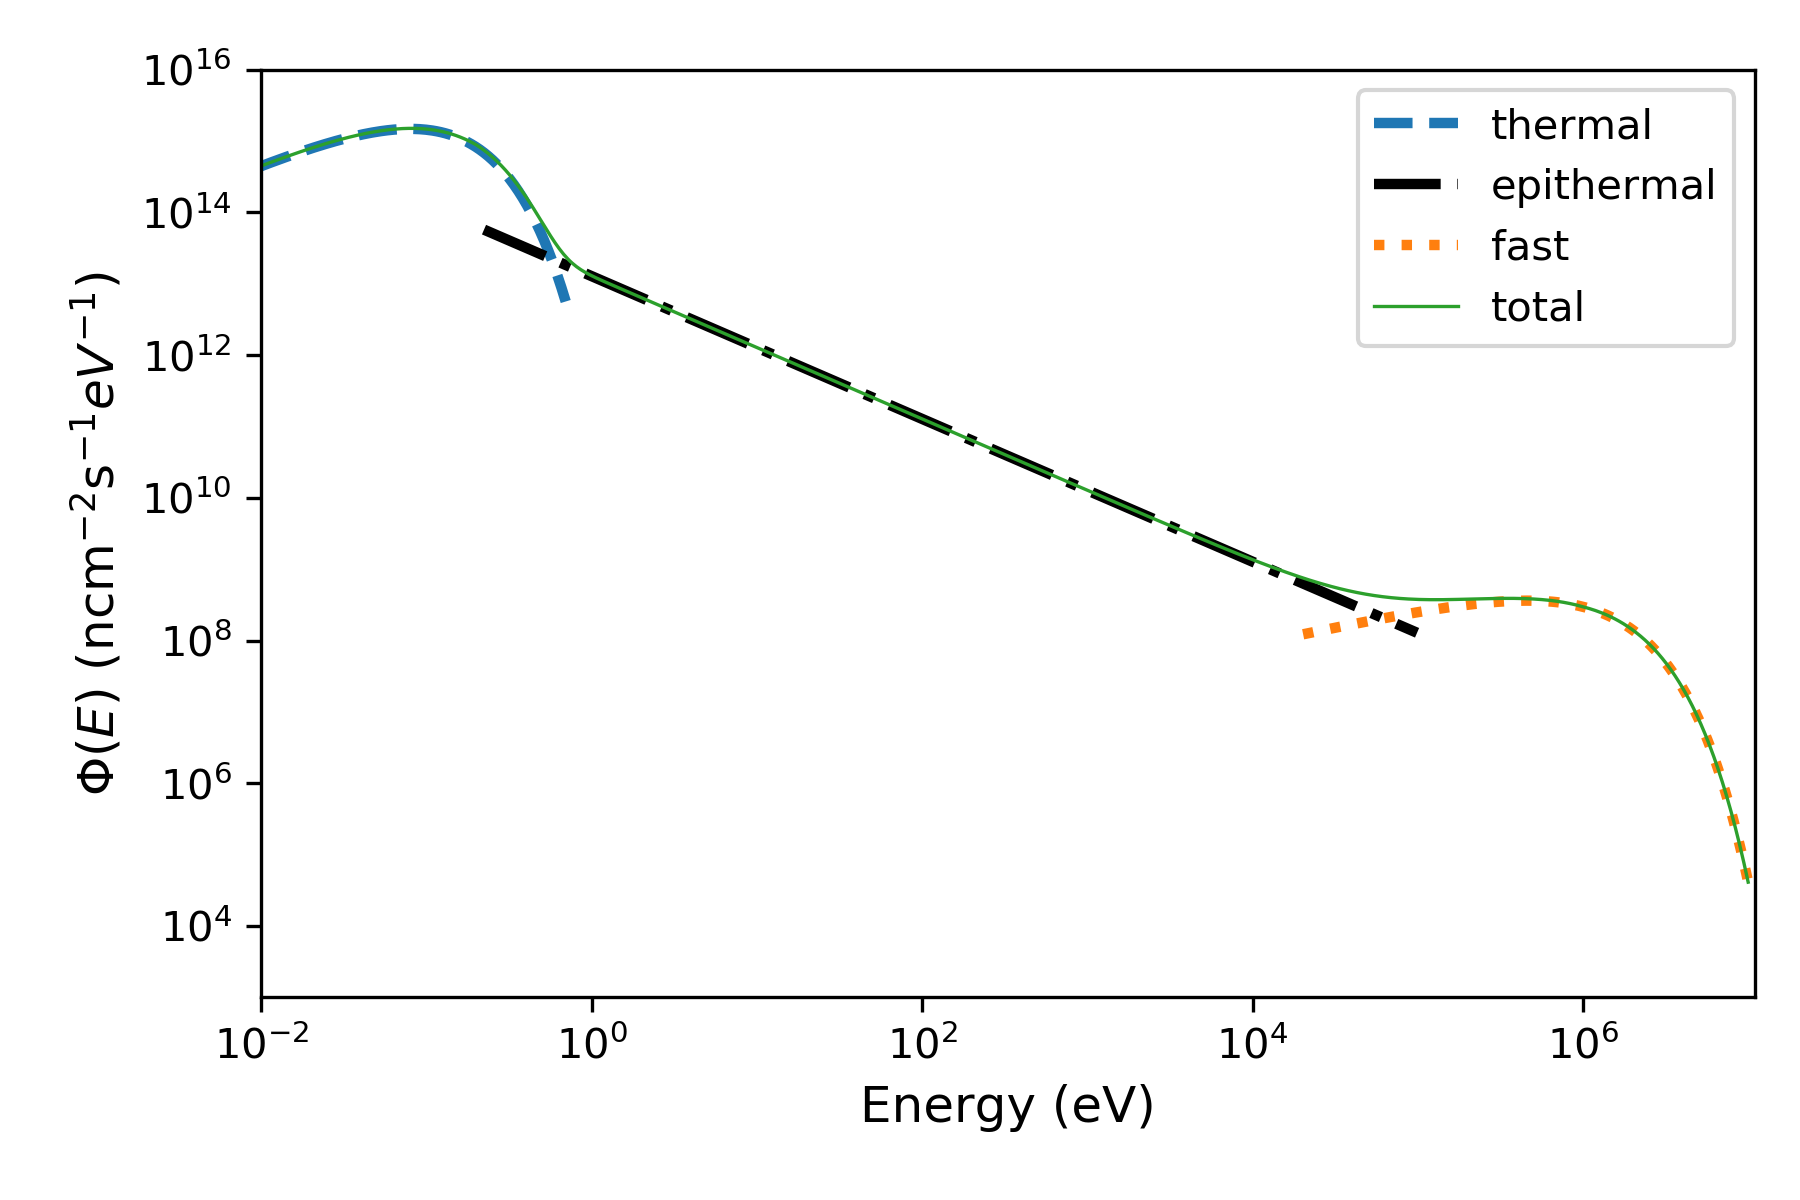
\includegraphics[scale=0.44] {figures/03-theoryspectrum.png}
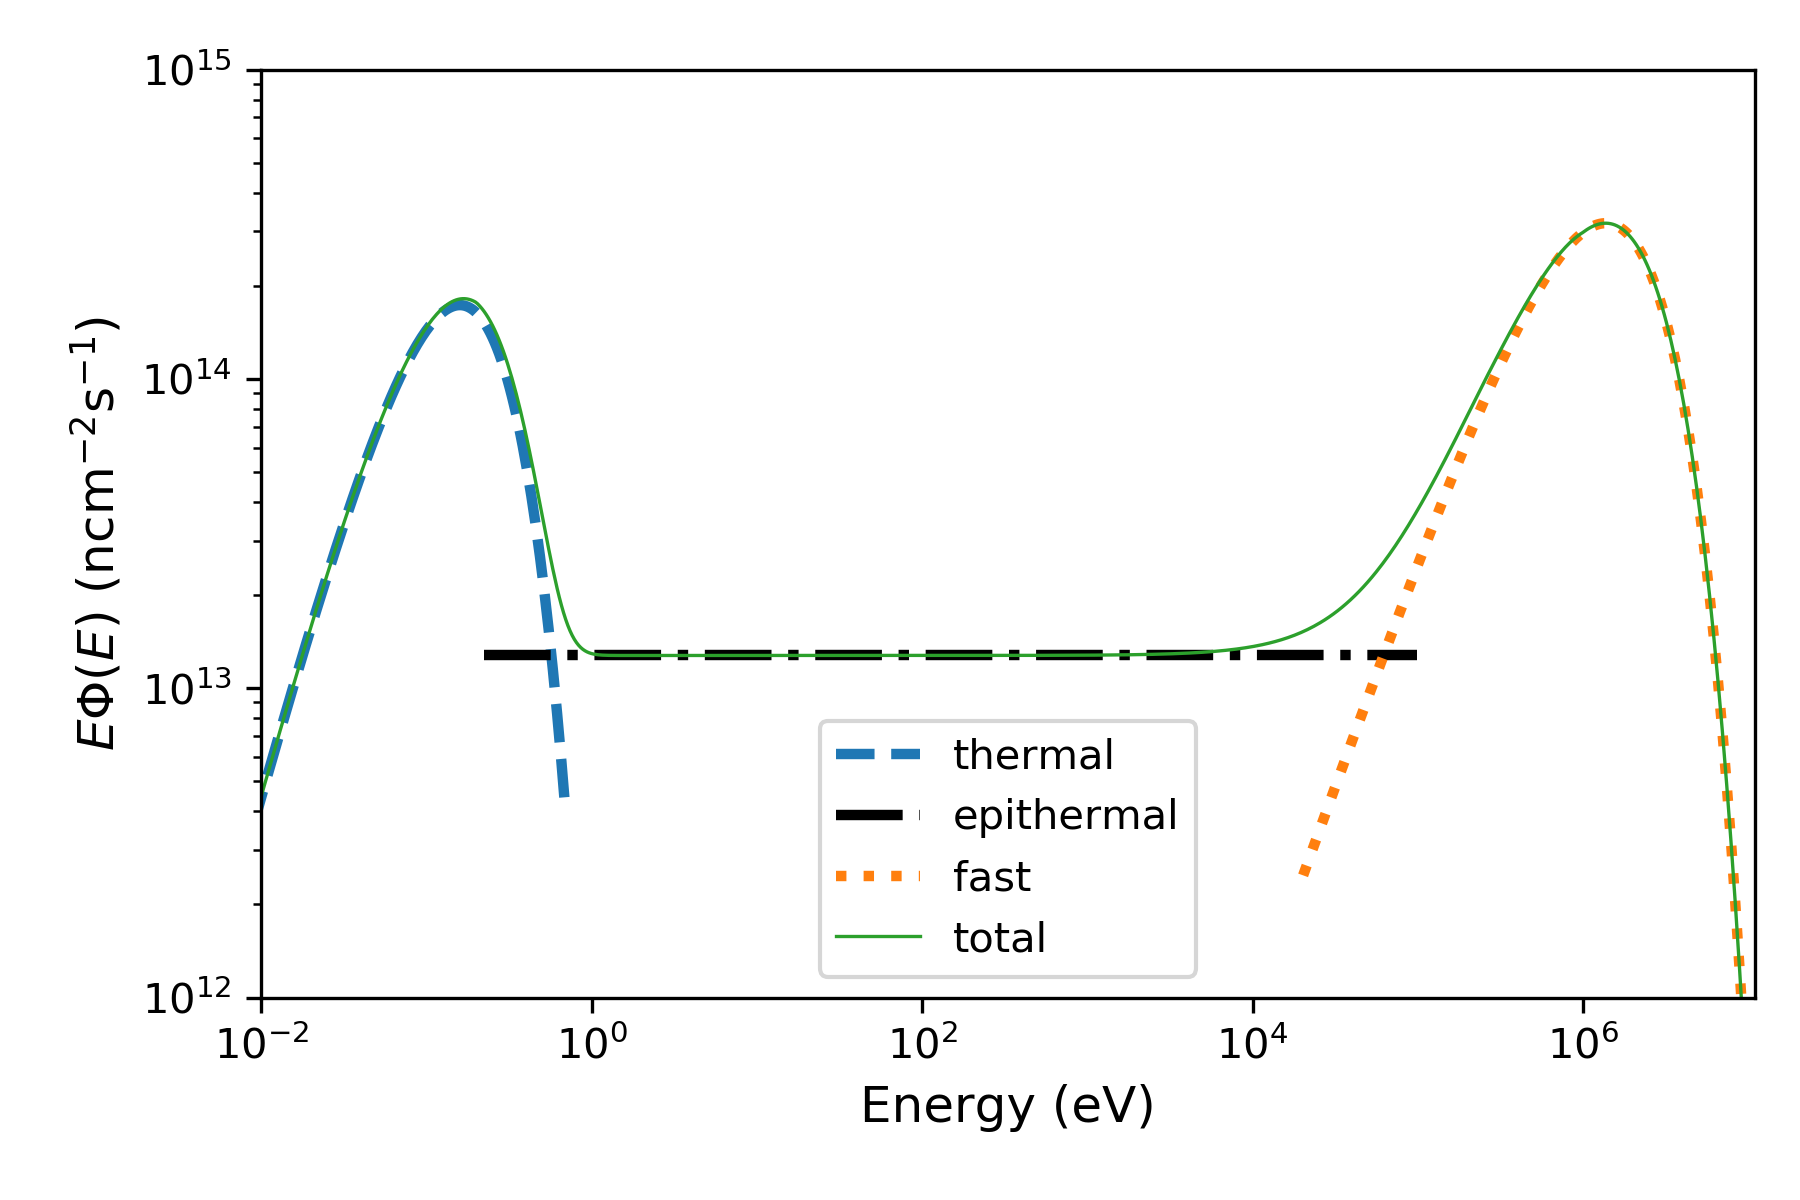
\includegraphics[scale=0.44] {figures/03-theoryspectrumlet.png}}\protect
\caption{\label{fig:idealneutronspectrum} \footnotesize{Idealized neutron spectrum.}}
\end{figure}

In the discussions of slowing down an other quantity is often introduces, the \textit{slowing down density}, which in our case is

$$q(E)=q(u)=\xi\Sigma_t\Phi(u)$$,

which gives the number of neutrons per unit time passing a certain lethargy (or energy). It is possible to give a more formal mathematical expression defining this quantity, and the interested reader is referred to D\&H (p321). However, we will your in our rather simplistic discussions.


\vspace{0.5cm}

\textbf{Slowing down on Hydrogen in the presence of absorbers}

Let us consider a case more relevant for reactor physics: a homogeneous mixture of hydrogen and heavy absorber nuclei (eg. uranium nuclei). We can notice from Table \ref{tab:moderator} that slowing down on the heavy nuclei can be neglected compared to the slowing down on hydrogen, thus in Eq. \eqref{eq:scatkernel} it is enough to consider hydrogen (for which $\alpha=0$) However, resonance absorption might occur when a neutron interacts with a heavy nucleus. 

With some laborious derivation (see for example Stacey's book) one can arrive to

\begin{equation}\label{eq:slowingdownHU}
 \Phi(E) = \frac{\Sigma_A^U(E_1) + \Sigma_S^H(E_1)}{ \Sigma_A^U(E) + \Sigma_S^H(E)} \cdot \frac{E_1\phi(E_1)}{E} \cdot \mathrm{exp}\left[-\int_E^{E_1} \frac{1}{E'} \frac{\Sigma_A^U(E')}{\Sigma_A^U(E') + \Sigma_S^H(E')}dE'\right]
\end{equation}

\noindent which gives a relation of the flux at $E$, to the flux at a higher energy $E_1$. First of all we can note that the lethargic flux at any energy is proportional to the lethargic flux at an other energy $\Phi(E)E \propto \phi(E_1)E_1$. And the proportionality is given by two factors: the first one is the ratio of the cross sections (absorption of uranium and scattering of hydrogen) at the respective energies; the second, exponential term which includes an integral from $E$ to $E_1$. The integral will always be positive therefore the exponential will be between 0 and 1, hence can be interpreted as a probability. 

We can consider three cases for $E$ and $E_1$:

1. The two energies are between resonances ($E_{r1}<E<E_1<E_{r2}$). Then the cross sections are close to constant, hence the first term $\approx 1$. And due to the scattering cross section of hydrogen is much larger than the absorption cross section of uranium, the exponent also becomes $\approx 1$. Therefore, we can conclude that  

$$\phi(E) \approx \frac{E_1\phi(E_1)}{E}$$

\noindent thus the lethargic flux is constant, and this is exactly what we have observed previously for the case when only scattering was considered.

2. When the energy is at a resonance $E_r=E<E_1$, the absorption cross section is much higher than the scattering. therefore the first term will become much smaller than 1. Since we know that the exponent is between 0 and 1, it will not influence our qualitative finding that 

$$\phi(E)E \ll \phi(E_1)E_1$$

\noindent the flux is greatly decreased at the resonance energy as illustrated in Figure~\ref{fig:selfshielding} for the notable resonance of U-238 at 6.67 eV. Neutrons that are scattered into the energy range of the resonance are absorbed, but those neutrons that scatter from energies above the resonances to energies below the resonances are not affected. However, due to the reduction in the flux, rate of resonance absorption also decreases, this is called \textit{energy self-shielding}.

\begin{figure}[ht!]
\protect \centering{
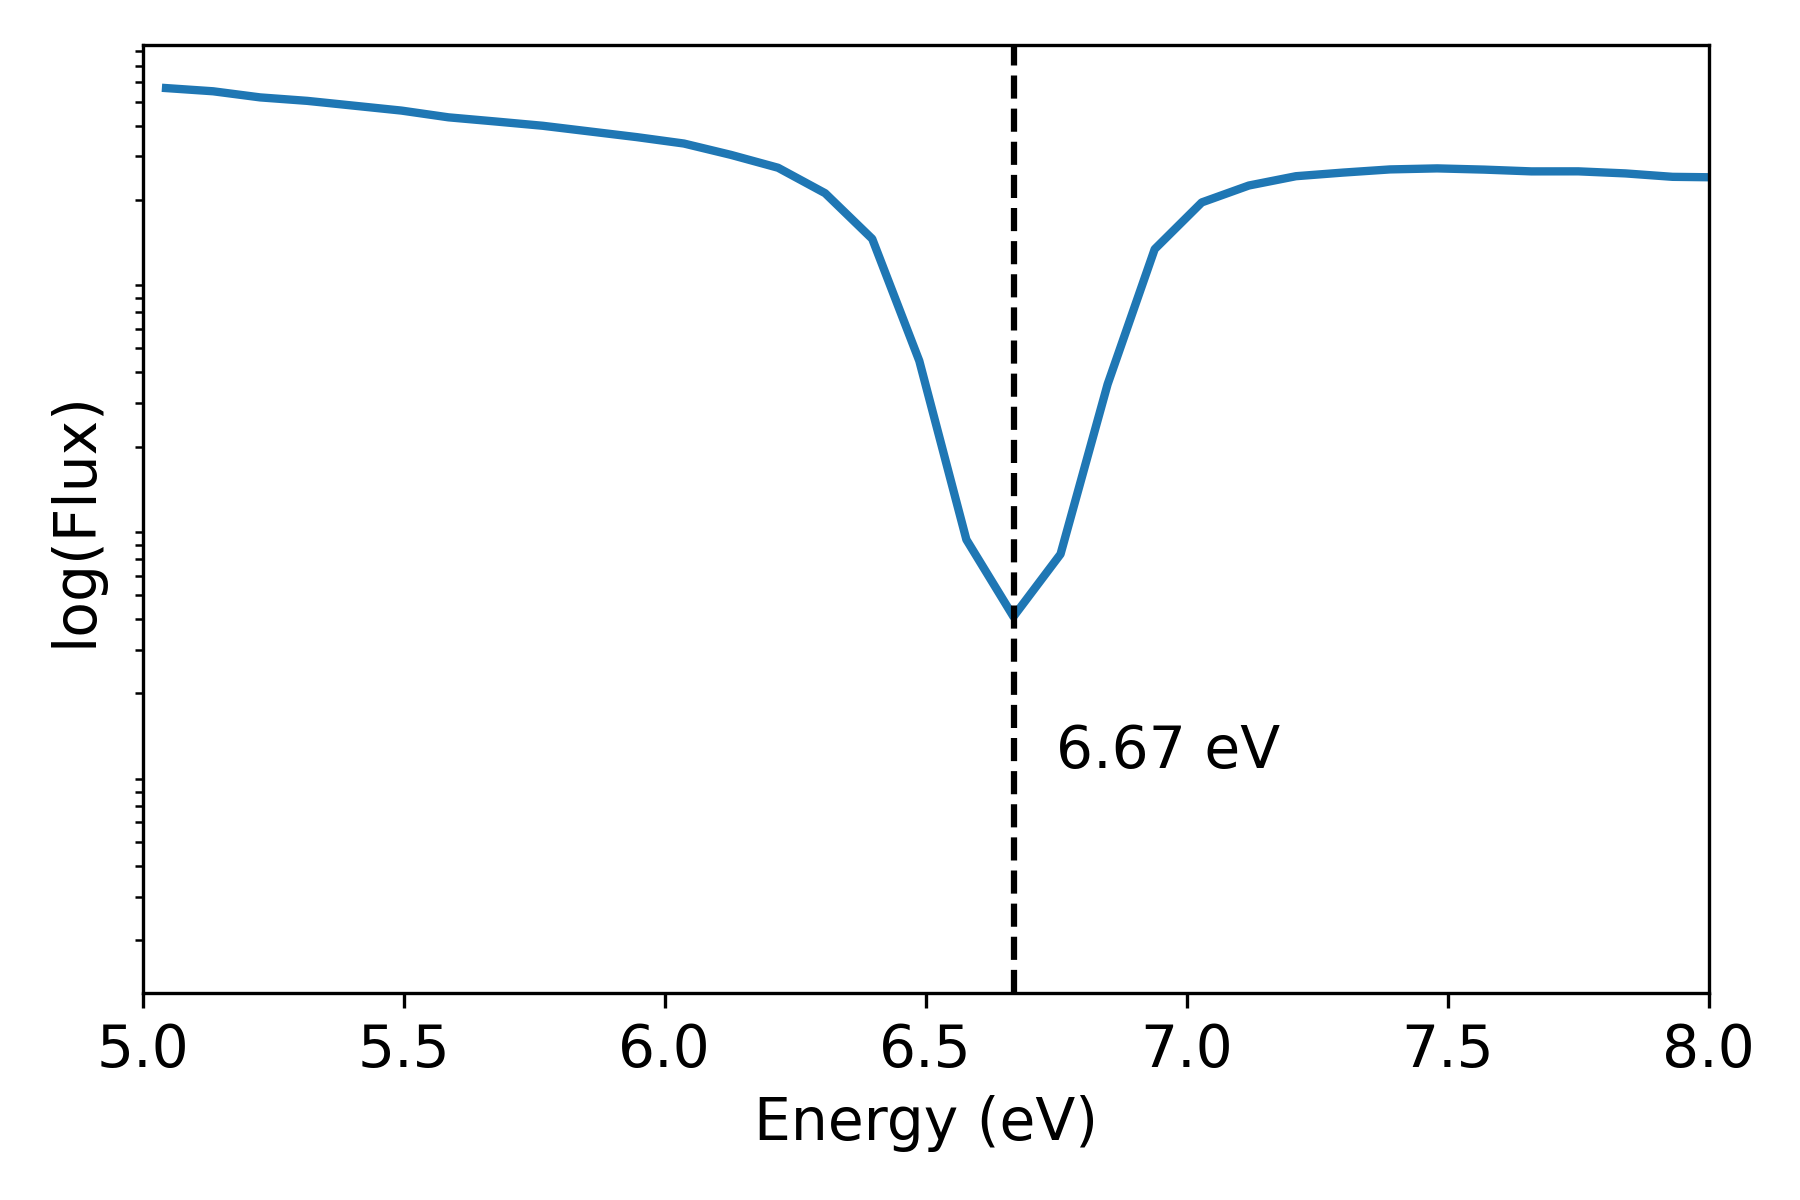
\includegraphics[scale=0.44] {figures/02-selfshielding.png}}\protect
\caption{\label{fig:selfshielding} \footnotesize{Resonance self-shielding.}}
\end{figure}
 
\begin{figure}[ht!]
\protect \centering{
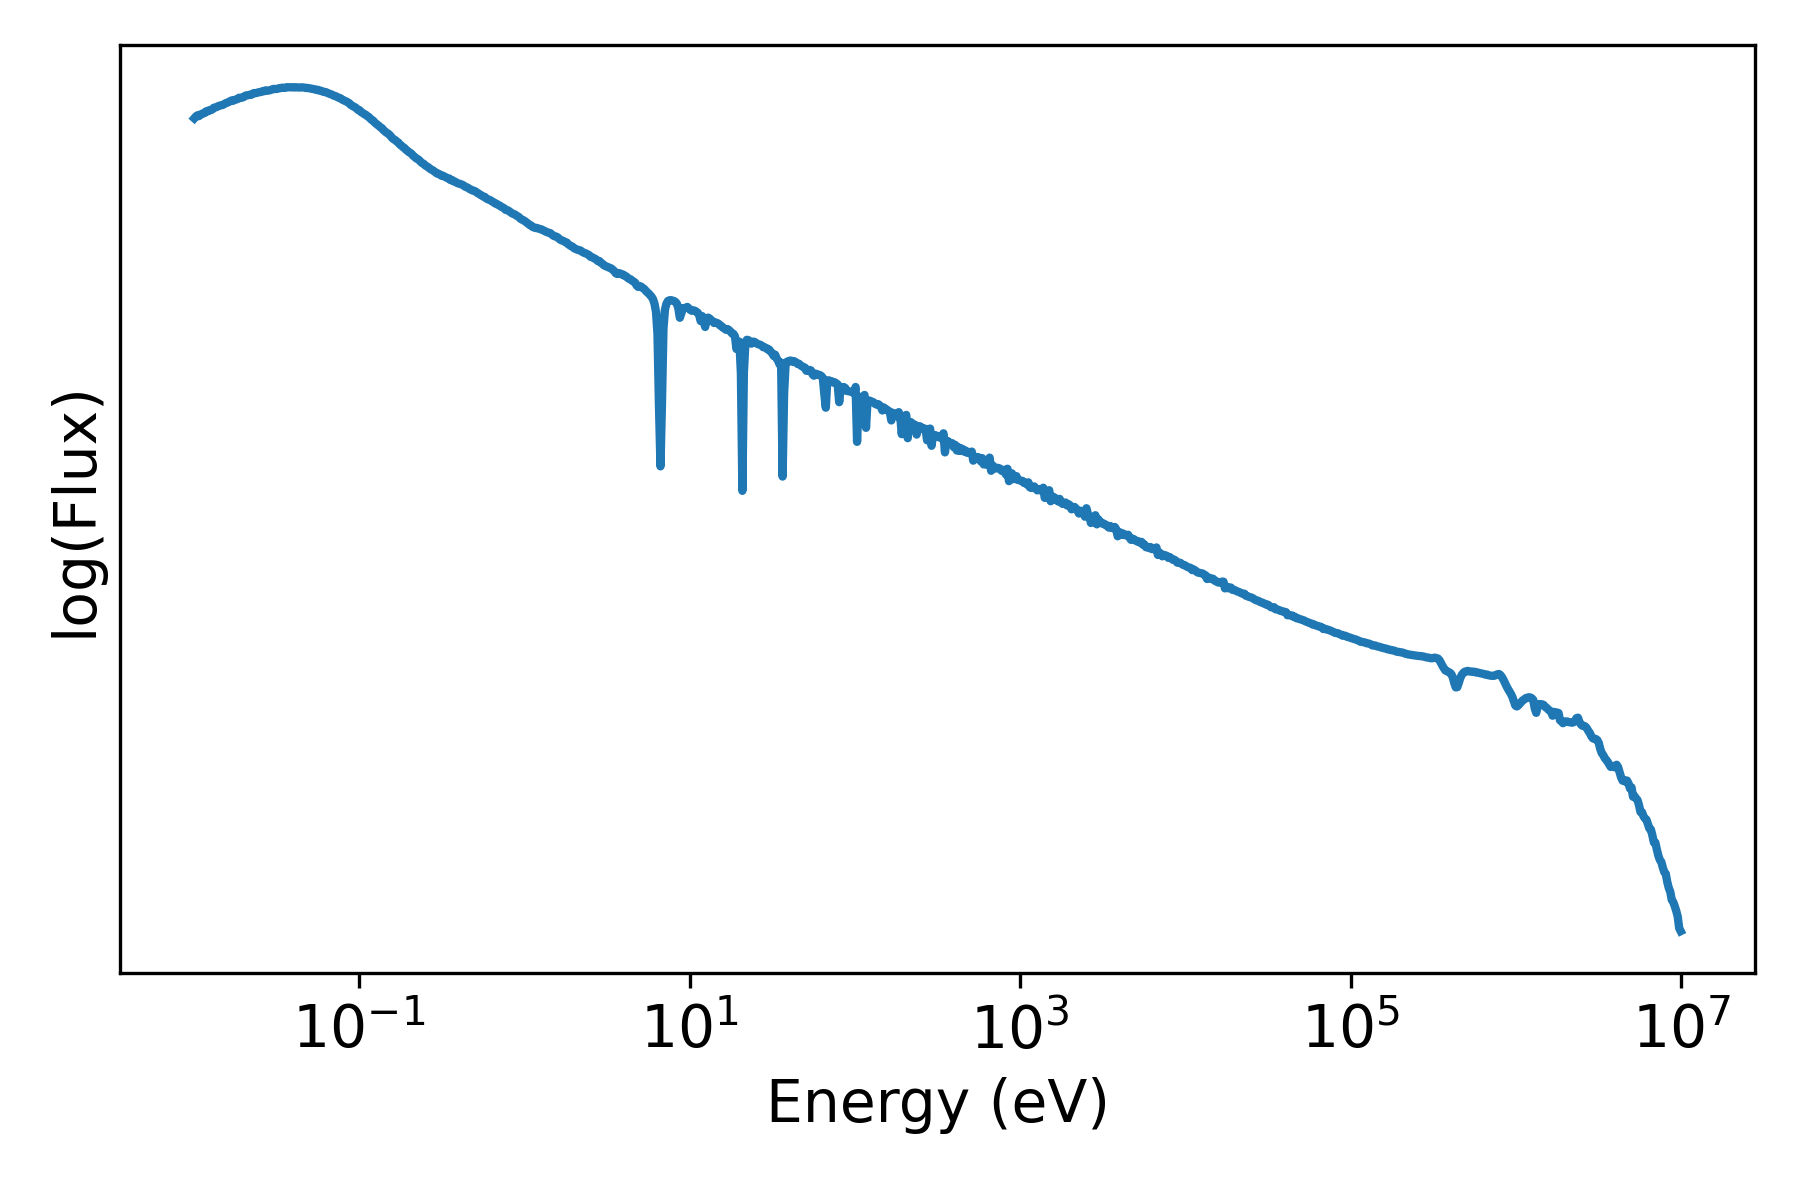
\includegraphics[scale=0.44] {figures/02-pwrspectrum.png}
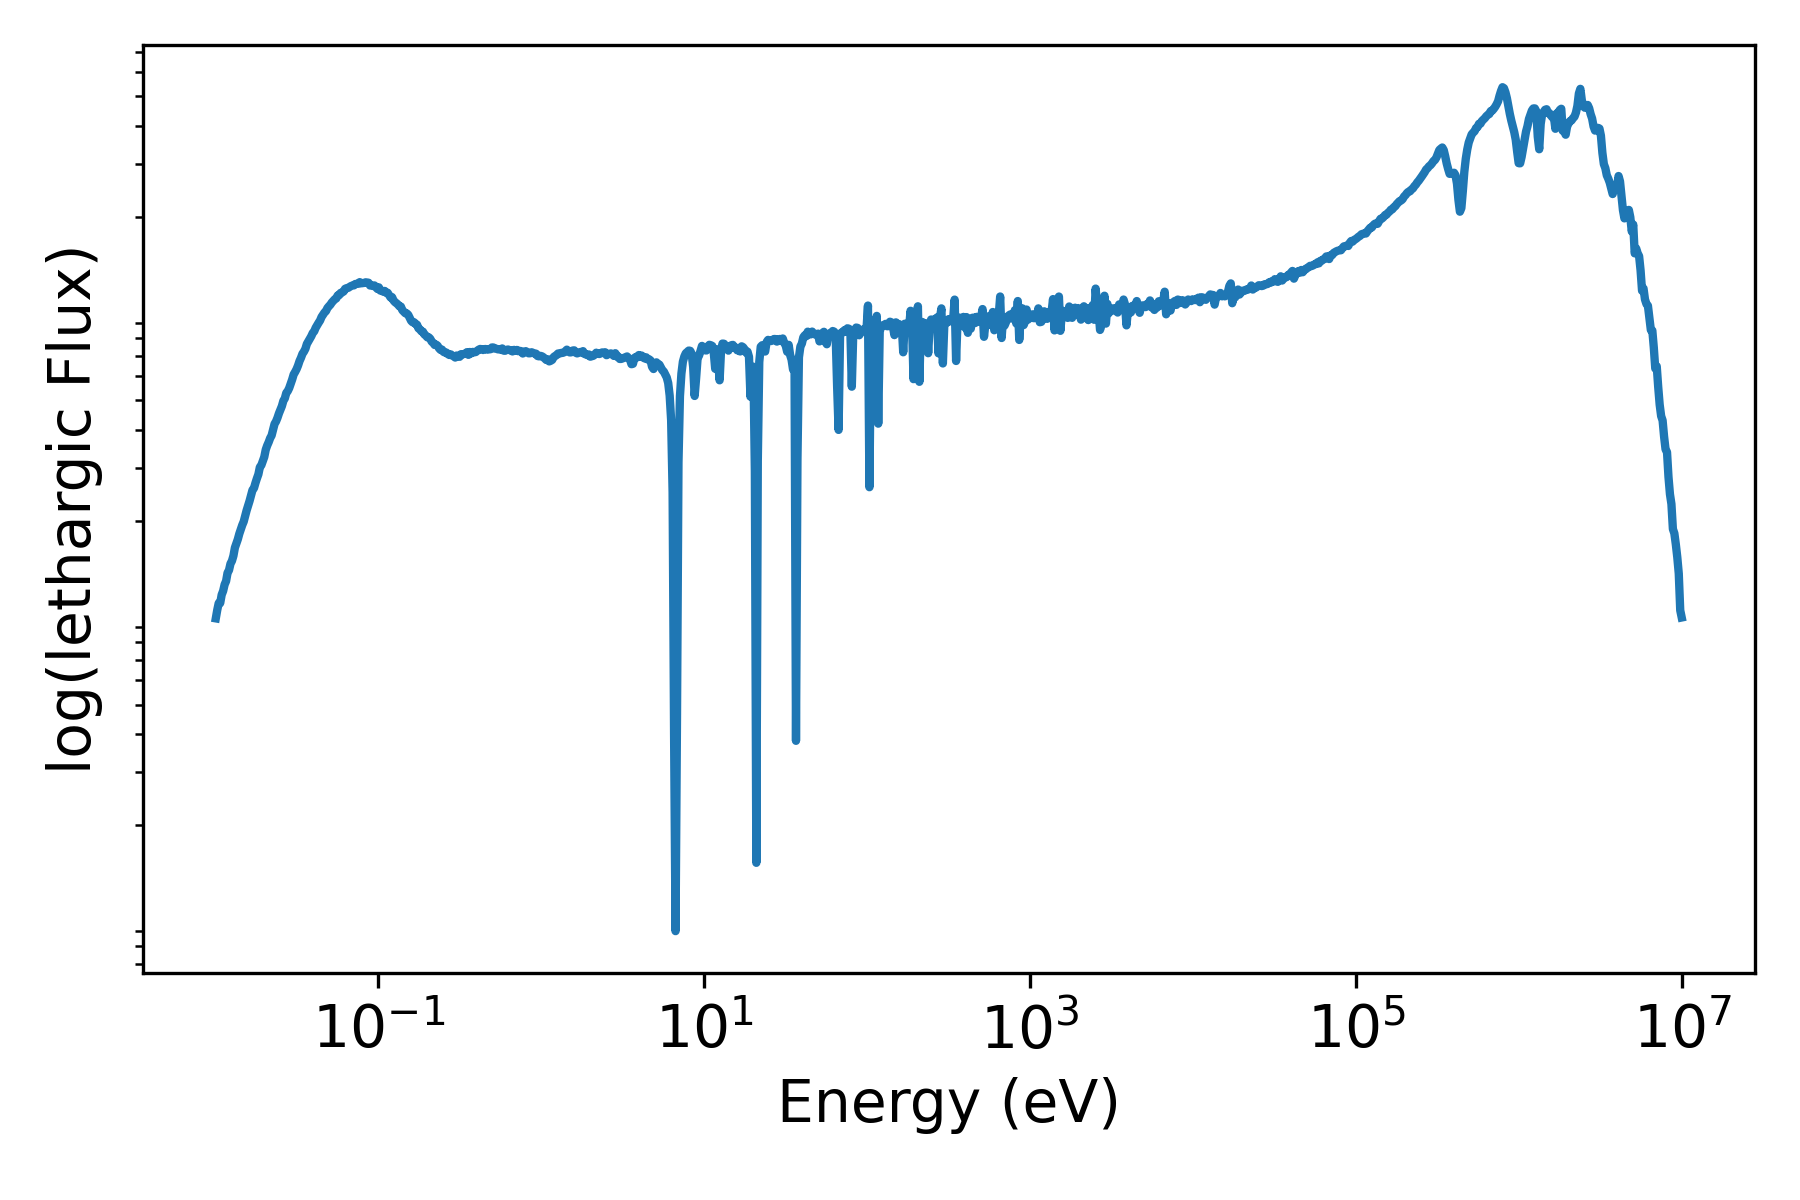
\includegraphics[scale=0.44] {figures/02-pwrspectrumlethargic.png}}\protect
\caption{\label{fig:realneutronspectrum} \footnotesize{PWR neutron spectrum ($\Phi(E)$ and $E\Phi(E)$).}}
\end{figure}

3. When the energies are separated by a resonance $E<E_r<E_1$, the first term is again close to unity, however the exponent is slightly less than~1 depending on the resonance width, which implies that the neutron flux is lower at the low energy side of the resonance compared to the high energy side. This is called \textit{resonance shielding}.

Figure \ref{fig:realneutronspectrum} illustrates the spectrum and the lethargic spectrum for a PWR calculation. We can recognize the above mentioned regions: Maxwell-distribution at thermal energies, the source Watt-distribution at fast energies with some influence from inelastic scattering, the close to $1/E$ trend in the slowing down region with the self-shielding effects.

\subsubsection{Resonance escape probability}

The probability appearing in Eq. \eqref{eq:slowingdownHU} if integrated over several resonances 

$$p(E_S\rightarrow E)=\exp\Bigg(-\int\limits_E^{E_S}\frac{\Sigma_a(E')}{E'\Sigma_t(E')}dE'\Bigg)$$

is called resonance escape probability, because it gives the ratio of neutrons which were not absorbed by the resonances while slowing down from $E_S$ to $E$.

$$\frac{S-\int\limits_E^{E_s}\Sigma_a(E')\Phi(E')dE'}{S}=p(E_S\rightarrow E)$$

Let's recall the phenomena of Doppler-broadening (ie. that the height of the resonance decreases while the width of the resonance increases with temperature), although the area under the resonance is constant, neutrons slowing down in discrete steps will have a higher probability to interact with the resonance, therefore the resonance escape probability $p$ decreases as the temperature increases. This, as we will see later when discussing feedback mechanisms, has an important implication on reactor safety: with increasing power, therefore increasing temperature the negative feedback of the Doppler-effect reduces the power.

% FOR FUTURE: RESONANCE INTEGRALS!!!
%The slowing down equation \ref{eq:slowingdown} becomes
%
%$$\int\limits_E^{\infty} \Phi(E')\frac{\Sigma_s(E')}{E'}dE'+S(E)=\Sigma_t(E)\Phi(E)$$
%
%\noindent where $\Sigma_s$ includes only the moderator, but $\Sigma_a$ (hidden in $\Sigma_t$) includes both the moderator and the heavy absorber. After differentiation one arrives to
%
%$$\frac{dF(E)}{dE}+\frac{\Sigma_s(E)}{E\Sigma_t(E)}F(E)=\frac{dS(E)}{dE}$$
%
%\noindent with introducing again the collision density $F(E)=\Sigma_t(E)\Phi(E)$. Of course we need some initial conditions for the differential equation. This we can get by considering that the source might have a maximum energy $E_max$ (for a monoenergetic source this would be obvious, for the Watt-spectrum we can safely assume this to be 10 MeV). Therefore the absorption rate above this energy is
%
%$$\int_{E_{max}}^\infty\Sigma_a(E)\Phi(E)dE=0$$
%
%\noindent which requires the flux, and therefore the collision density to be zero above this energy.
%
%$$F(E)=0 \: \text{for} \: E\geq E_{max} $$
%
%Here we will omit deriving the solution (it can be found in books). Just present the rather involved result
%
%$$F(E)=S(E)+\frac{1}{E}\int\limits_E^\infty S(E')\frac{\Sigma_s(E')}{\Sigma_t(E')}\exp\Big(-\int\limits_E^{E'}\frac{\Sigma_a(E'')}{E''\Sigma_t(E'')}dE''\Big)dE'$$ 
%
%\noindent but as probably at this point we are already used to this, we can make some reasonable assumptions to simplify this result.

%As mentioned before, in our discussion we are going to make serious assumptions: we will be studying slowing down in an infinite medium where a monoenergetic source emits neutrons uniformly. We also consider that elastic scattering is isotropic (therefore, we know that our derivations will be close to reality only below 100 keV).
%
%When discussing slowing down it is convenient to introduce two quantities:
%
%$$F(E)=\Sigma_S(E)\phi(E)=\text{collision density}$$
%
%\noindent which gives the number of collision per unit volume, unit time and unit energy in the energy bin $[E,E+dE]$. Notice that in fact this is a reaction rate-like quantity.
%
%$$q(E)=\text{slowing-down density}$$
%
%\noindent which gives the number of neutrons per unit volume and per unit time whose energy falls below $E$.
%
%Then we will discuss slowing-down for two cases: without and with absorption. And we will assume that the energies are well below the energy of the source.  We also require for the derivation that we are in the asymptotic region ($E<\alpha^3E_0)$), since close to the energy of the source, it is undetermined how many collisions are required to reach energy $E$. It might take one or more collisions. However, energies well below the source energy, we can assume that neutrons cannot reach directly.


\subsection{Neutron cycle: 4 factor formula}

We have previously developed a simple $2 factor$ model to estimate the multiplication factor $k$. Since then however we have studied the neutron spectrum, and discussed how neutrons are slowing down, and if they escape the resonance region then might reach thermal energies and cause fission, therefore we can give a more appropriate model for the neutron cycle that is when neutrons are born in fission, slow down, and might initiate fission thus giving birth to a new generation of neutrons as being illustrated in Figure \ref{fig:neutroncycle}.

Up to now we have considered homogeneous reactors, but in order to accommodate that in actual reactors the fuel and the moderating material is well separated (for an LWR in the form of fuel rods and coolant channels), we will consider a space and energy dependent flux $\phi(\mathbf{r},E)$ in the following.

\begin{figure}[ht!]
\protect \centering{
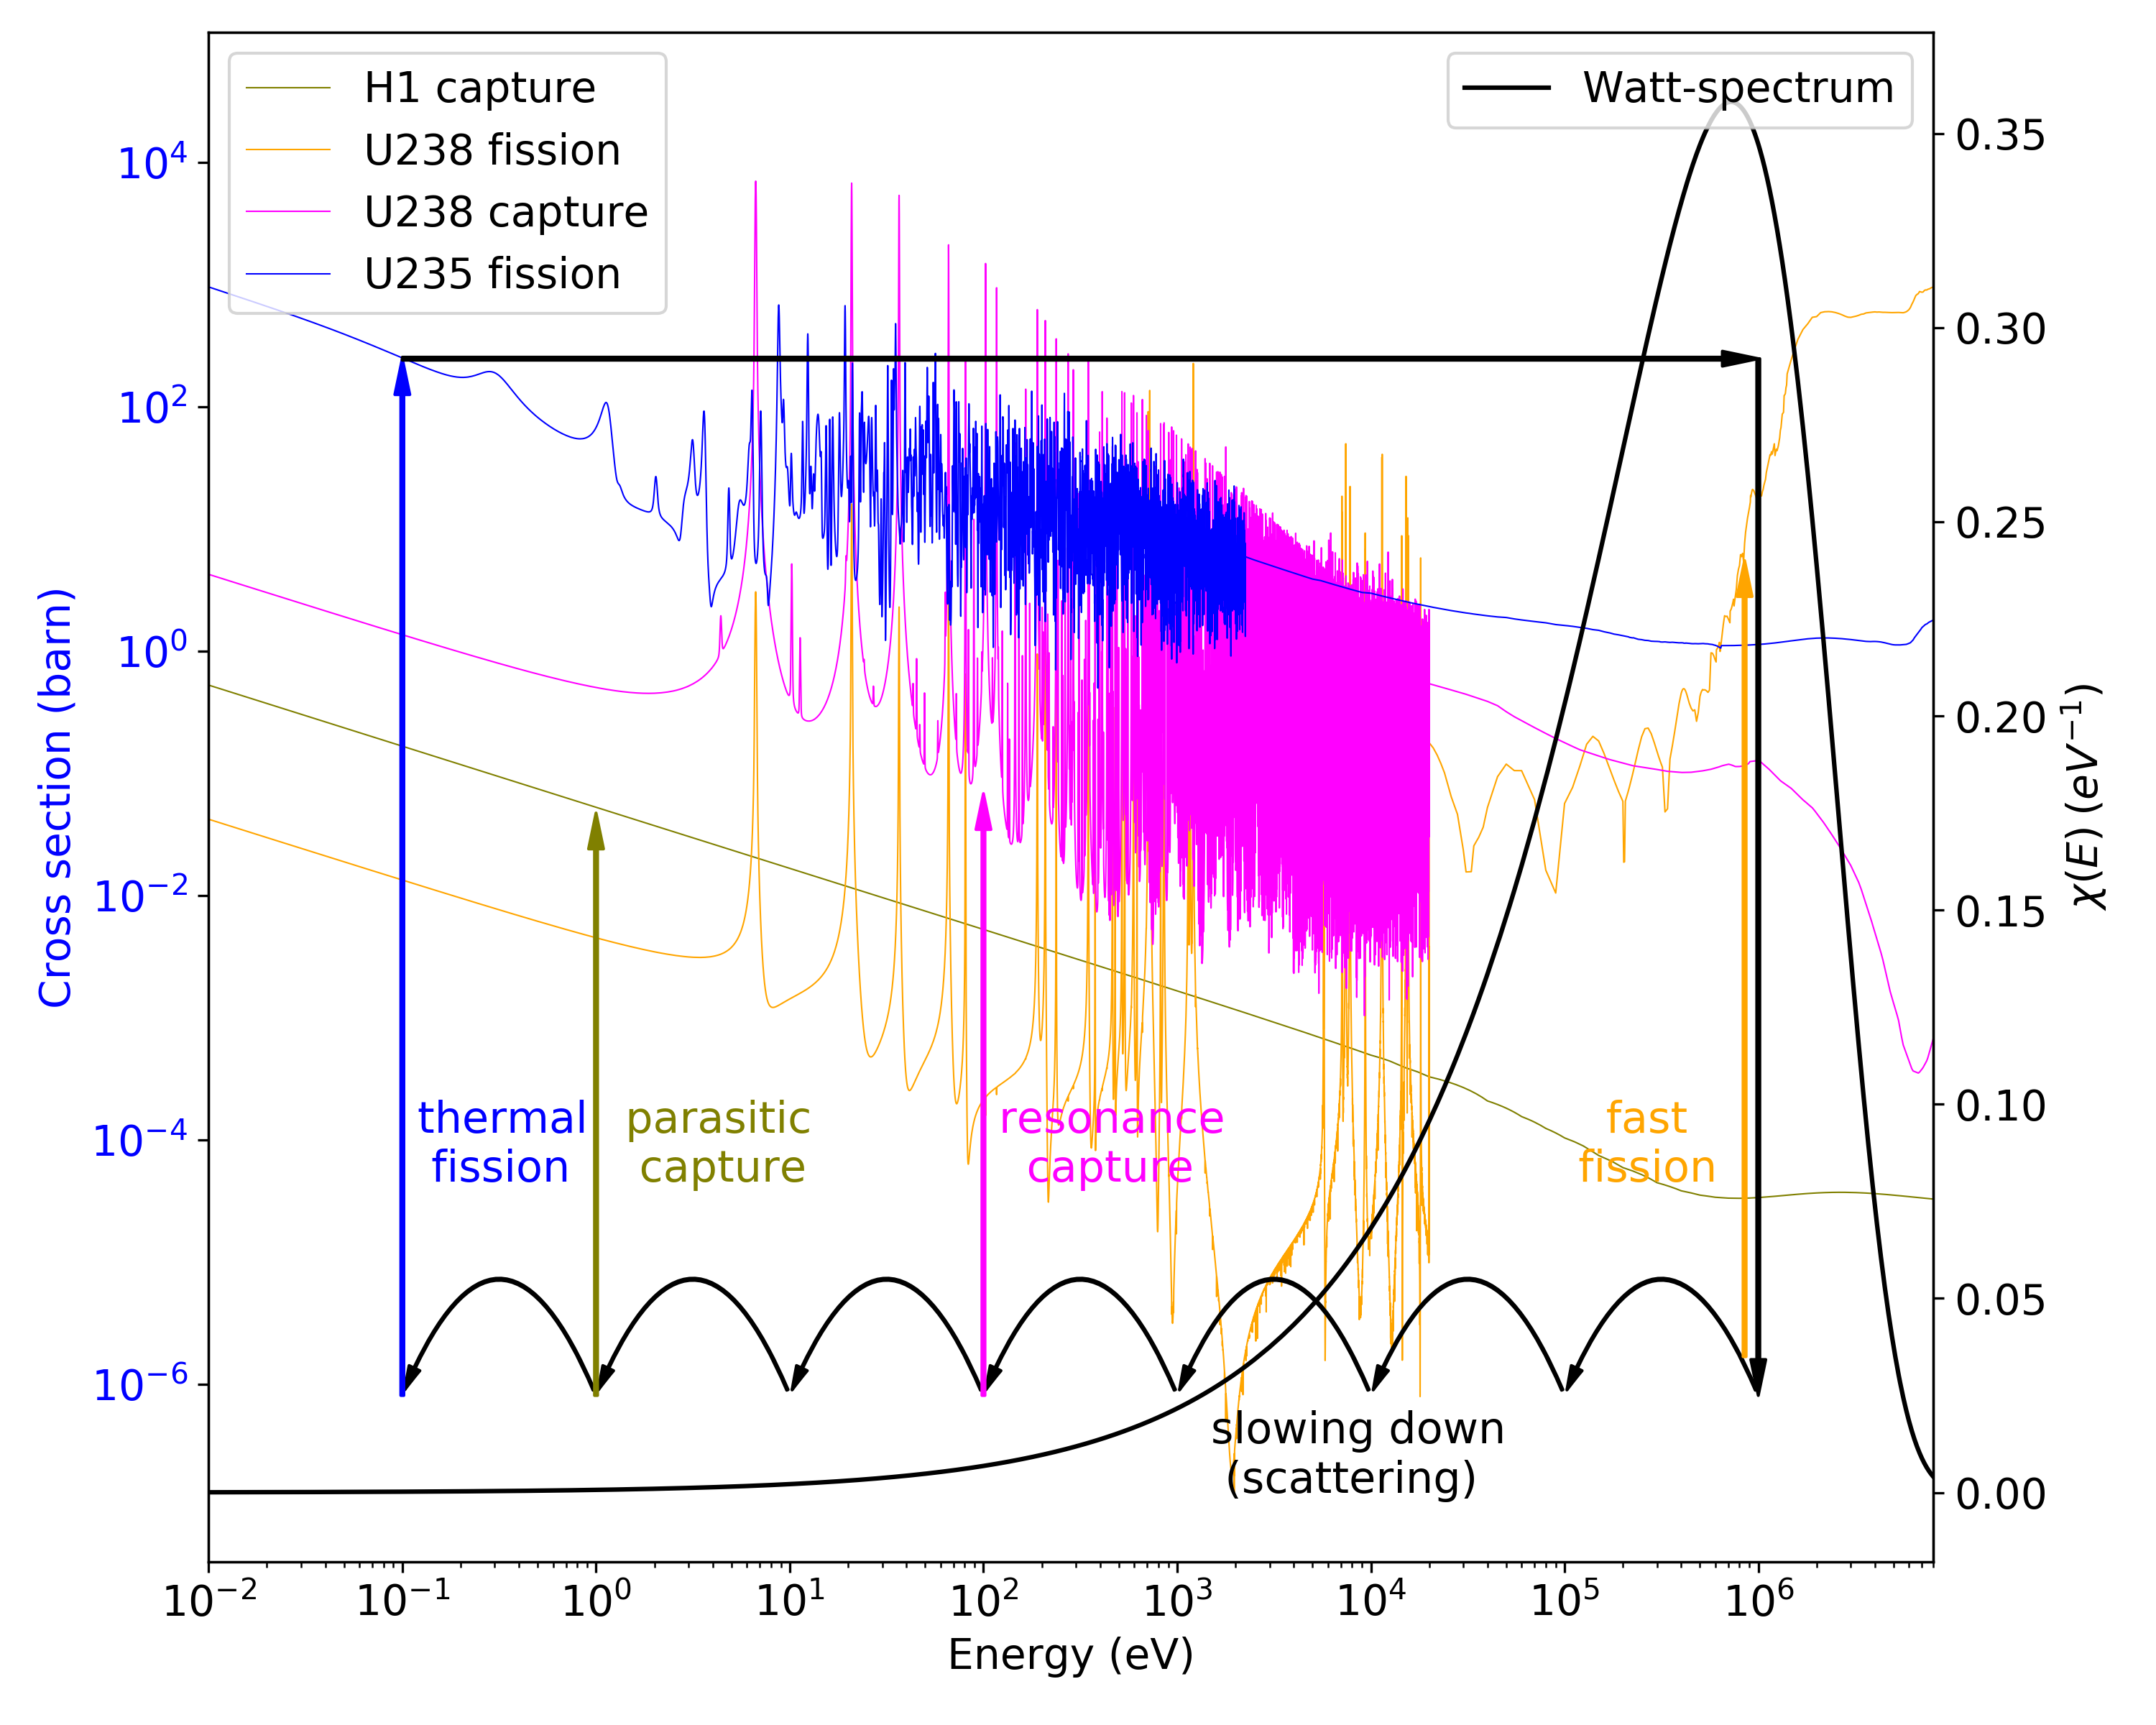
\includegraphics[scale=0.54] {figures/03-neutroncycle.png}}\protect
\caption{\label{fig:neutroncycle} \footnotesize{Schematic representation of the neutron cycle.}}
\end{figure}

At the beginning of the cycle neutrons are born at high energies. As we have previously noted, certain nuclides such as U-238 have a threshold for fission with high energy neutrons, thus in fact some of the neutrons are born due to fast fission. This is characterized by the \textit{fast fission factor}, 

$$\epsilon=\frac{\int_{V_{F}} \int_0^\infty \nu(E)\Sigma_f(\mathbf{r},E)\phi(\mathbf{r},E)dVdE}{\int_{V_{F}} \int_0^{\sim 5kT} \nu(E)\Sigma_f(\mathbf{r},E)\phi(\mathbf{r},E)dVdE}$$

\noindent which characterizes the ratio of the number of neutrons born in fission (due to both thermal and fast neutrons) and the number of neutrons born in fission induced by thermal neutrons.

Then, after birth the neutrons will slow down mainly due to elastic scattering events. The \textit{resonance escape probability} 

$$p=1-\frac{\int_{V_{F}} \int_{\sim 5kT}^\infty \Sigma_a(\mathbf{r},E)\phi(\mathbf{r},E)dVdE}{\int_{V_{F}} \int_0^{\infty} \nu(E)\Sigma_f(\mathbf{r},E)\phi(\mathbf{r},E)dVdE}$$

\noindent characterizes the probability that neutrons while traveling through the epithermal region will not be absorbed by the resonances of the absorber nuclei. 

When the neutrons reach the thermal region, due to the $1/v$-behavior of the cross sections they will be absorbed either in the fuel or due to parasitic capture of other materials (eg. coolant or structural elements. As we saw earlier, the \textit{thermal utilization factor}

$$f=\frac{\int_{V_{F}} \int_0^{\sim 5kT} \Sigma_a(\mathbf{r},E)\phi(\mathbf{r},E)dVdE}{\int_{V_{total}} \int_0^{\sim 5kT} \Sigma_a(\mathbf{r},E)\phi(\mathbf{r},E)dVdE}$$

characterizes the ratio of the number of thermal neutrons absorbed in the fuel and the number of thermal neutrons absorbed in other materials.

Finally, neutrons which are absorbed by the fuel might induce fission from which new neutrons emerge or are captured by the nuclei. The \textit{thermal fission factor}

$$\eta=\frac{\int_{V_{F}} \int_0^{\sim 5kT} \nu(E)\Sigma_f(\mathbf{r},E)\phi(\mathbf{r},E)dVdE}{\int_{V_{F}} \int_0^{\sim 5kT} \Sigma_a(\mathbf{r},E)\phi(\mathbf{r},E)dVdE}$$

gives the average number of fission neutrons emitted per thermal neutron absorbed in the fuel.

By multiplying these values we can calculate the infinite multiplication factor through the \textit{4-factor formula}

$$k_{\infty}=\eta f p \epsilon$$

In order to compute the k-effective, one needs to take into account the leakage, which is often given denoted separately for fast and thermal neutrons: $P_{FNL}$, $P_{TNL}$. However, it has to be highlighted again, that the determination of the non-leakage probabilities is rather complicated.

Today, the 4-factor formula is rather an educational tool to summarize the various processes in fission chain reactions, or to illustrate the impact of changing some parameter of the reactor (eq. temperature), and in practice it has little use. Nevertheless, before computers could have been used for elaborate calculations, this formula was the basis of reactor physics: the factors were determined from measurements, and then the formula was used to determine the multiplication factor.

However, as we will see in the next Chapter, today we can use more elaborate methods to estimate the multiplication factor.

%\end{document}

%\documentclass[12pt]{article}
%\usepackage{amsmath}
%\usepackage{graphicx, color}
%\usepackage{amssymb}
%\usepackage{listings} %source code listing
%\usepackage{multirow}
%%\usepackage[version=2]{mhchem}
%\usepackage{subfig}
%\usepackage{hyperref}
%\usepackage{units}
%\usepackage{gensymb}
%\usepackage{adjustbox}
%\usepackage{listings}
%\usepackage{color}
%\usepackage{tcolorbox}
% 
%\definecolor{codegreen}{rgb}{0,0.6,0}
%\definecolor{codegray}{rgb}{0.5,0.5,0.5}
%\definecolor{codepurple}{rgb}{0.58,0,0.82}
%\definecolor{backcolour}{rgb}{0.95,0.95,0.92}
%
%\newcommand{\specialcell}[2][c]{%
%  \begin{tabular}[#1]{@{}c@{}}#2\end{tabular}}
% 
%
%
%\title{Reactor physics with Python \\ Lecture Notes}
%
%
%\author{Zs.~Elter. E. Branger, M. Preston \\ Uppsala University \\
%        Division of Applied Nuclear Physics}%\corref{cja}}
%%
%\date{2021.}
%\begin{document}

\section{Neutron transport and diffusion}

In this section we are going to derive an equation describing neutron transport in general. This equation is the basis of reactor physics, and can be approximated in several ways to study only certain parts of neutron physics.

Several course books introduces neutron transport immediately by jumping into neutron diffusion and considering that neutrons move around in materials or in a reactor as gas molecules would. In this case one assumes that neutrons tend to diffuse from regions of high neutron density to regions of low neutron density (which is qualitatively usually true, but the quantitative relation ship between flux and current density is where the approximation comes in). One reason for this approach is that solving the neutron transport equation is intimidating, or in most realistic cases it is even impossible, whereas handling the diffusion formalism is more straightforward.

However, deriving the exact neutron transport equation is actually simpler than deriving the diffusion equation, and since it describes reality better, it is actually worth to start from here, and later turn our attention towards diffusion which is an approximations of neutron transport theory. Therefore after deriving the general transport equation we will simplify it to reach the diffusion theory, which we will use to have a basic understanding of the spatial distribution of neutrons in a reactor core.

The main goal of neutron transport, and thus this chapter is to tracking the population of neutrons at any point of the reactor, thus determine the neutron population

\begin{equation}
n(\mathbf{r}, E, \mathbf{\Omega},t) = \:?
\end{equation}

\noindent and to develop a balance equation for the population

\begin{equation}
\frac{\partial n(\mathbf{r}, E, \mathbf{\Omega},t)}{\partial t} = \:? = \text{gains} - \text{losses}
\end{equation}

The main focus of neutron transport is to figure out how to solve for the neutron population density $n(\mathbf{r}, E, \mathbf{\Omega},t)$. If we know this, we will know the location and velocity of all neutrons at all time. To achieve this, we will need to know the reaction rates which can take remove and add neutrons to the system. For all reactions there is an associated change in energy (except forward scattering which is basically a "miss"), change in momentum and direction.

The balance equation is not going to be difficult. We have only couple of reactions which result in "gain" reactions. And when it is about losses, it is really just the total cross section which will come to play, since essentially all reactions result in a loss of a neutron at the certain phase space. Besides this we will have streaming terms: neutrons without reaction might come into our infinitesimal volume and might leave it, and we will be interested in the net outcome of these streaming movements. Nevertheless, as we will soon see, even though the equations developed are rather intuitive and straightforward, their solutions are challenging.

\subsection{Basic quantities: neutron density, flux and current}

In order to describe the population of neutrons in a reactor we will need to introduce several quantities (some of which we have already introduced, although not in their most generic form). In the following we summarize the related chapter of D\&H (p122), and the reader is definitely encouraged to read that for further details.

\begin{figure}[ht!]
\protect \centering{
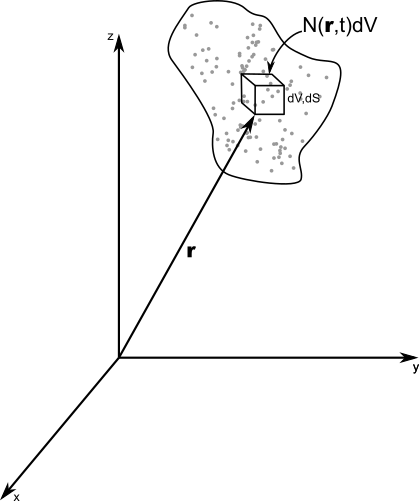
\includegraphics[scale=0.66] {figures/03-neutronpopulation.png}}\protect
\caption{\label{fig:neutronpopulation} \footnotesize{Illustration of neutron population density.}}
\end{figure} 

Let us define the expected number of neutrons in $dr^3$ about $\mathbf{r}$, energy $dE$ about $E$ moving in direction $\mathbf{\Omega}$ in solid angle $d\mathbf{\Omega}$ at time $t$ as the angular neutron population density

\begin{equation}
n(\mathbf{r},E,\mathbf{\Omega},t)dr^3dEd\mathbf{\Omega}
\end{equation}

\noindent Similarly we could define the scalar neutron population density after eliminating certain variables 

$$N(\mathbf{r},t)=\int^\infty_0N(\mathbf{r},E,t)dE=\int^\infty_0\int_{4\pi}n(\mathbf{r},E,\mathbf{\Omega},t)d\mathbf{\Omega}dE$$

\noindent which is illustrated in Figure \ref{fig:neutronpopulation}.

Then we can recall, that the actual physical quantity we can directly measure in a reactor is the reaction rate density (similar reaction rates can be defined for the energy integrated population density, or for the angular density):

\begin{equation}
R(\mathbf{r},E,t)dr^3dE=v(E)\Sigma(E) N(\mathbf{r},E,t)dr^3dE
\end{equation}

\noindent where, due to convenience we usually introduce the neutron flux (again, we can analogously define scalar and angular quantities)

\begin{equation}
\phi(\mathbf{r},E,\mathbf{\Omega},t)=v(E)n(\mathbf{r},E,\mathbf{\Omega},t)
\end{equation}

\begin{equation*}
\Phi(\mathbf{r},E,t)=v(E)N(\mathbf{r},E,t)
\end{equation*}

\begin{equation*}
\Phi(\mathbf{r},t)=vN(\mathbf{r},t)
\end{equation*}

\noindent where the relationship between the angular and scalar flux is

$$\Phi(\mathbf{r},t)=\int^\infty_0\Phi(\mathbf{r},E,t)dE=\int^\infty_0\int_{4\pi}\phi(\mathbf{r},E,\mathbf{\Omega},t)d\mathbf{\Omega}dE$$

Note that the neutron flux often has a "bad reputation", and the reason is that it is because it is not like other flux quantities we are used to from physics, since the neutron flux is a scalar quantity (even the angular flux is scalar, to cause some headache), whereas fluxes in eg. heat conduction are vectors. And although the neutron flux does have a physical interpretation (total distance traveled in a volume per second by neutrons going into a certain direction with a certain energy), it is due to mathematical convenience that we prefer to work with it. 

We can however introduce a quantity, the neutron current which rather corresponds to the conventional flux quantities. We can define the angular neutron current density

\begin{equation}
\mathbf{j}(\mathbf{r},E,\mathbf{\Omega},t)=\mathbf{\Omega}\phi(\mathbf{r},E,\mathbf{\Omega},t)
\end{equation}

\noindent and with that we can give the expected number of neutrons passing through an area $dS$ per unit time with energy $E$ in $dE$ and direction $\underline\Omega$ in $d\underline\Omega$ at time $t$:

$$\mathbf{j}(\mathbf{r},E,\mathbf{\Omega},t)dSdEd\mathbf{\Omega}$$

And again we can eliminate variables by integration

$$\mathbf{J}(\mathbf{r},t)=\int^\infty_0\mathbf{J}(\mathbf{r},E,t)dE=\int^\infty_0\int_{4\pi}\mathbf{j}(\mathbf{r},E,\mathbf{\Omega},t)d\mathbf{\Omega}dE$$

Note that $\mathbf{J}(\mathbf{r},t)dS$ is the net rate of neutrons passing through a surface area dS. The flux and the current density are similar, however the current density is a vector. That said the main difference is that the current density is the \textit{net} rate the neutrons pass through a surface oriented in a given direction, whereas the flux is the \textit{total} rate at which neutrons pass through unit area regardless its orientation. So $\mathbf{J}$ is more convenient to describe flow and leakage, whereas $\Phi$ is more convenient to describe reaction rate.

We can define the partial current density (total rates neutrons flow from left to right or right to left) as shown in Figure \ref{fig:partialcurrent}

$$J_\pm (\mathbf{r},t)=\int^\infty_0\int_{2\pi^\pm}\mathbf{e_s}\mathbf{j}(\mathbf{r},E,\mathbf{\Omega},t)d\mathbf{\Omega}dE \: \rightarrow \: \mathbf{e_s}\mathbf{J}(\mathbf{r},t)=[J_+(\mathbf{r},t)-J_-(\mathbf{r},t)]$$
 
Thinking about the current and partial currents will come handy at boundaries, where we for example want to satisfy the condition that there is no flow from one side of the boundary.

\begin{figure}[ht!]
\protect \centering{

\includegraphics[scale=0.46] {figures/partialcurrent.png}}\protect
\caption{\label{fig:partialcurrent} \footnotesize{Illustration of partial current.}}
\end{figure} 

As a final note we can mention that for isotropy the angular density is independent of $\mathbf{\Omega}$

$$n(\mathbf{r},E,\mathbf{\Omega},t)=\frac{1}{4\pi}N(\mathbf{r},E,t)$$


\subsection{Neutron transport equation}

Let us consider that we selected a beam of neutrons at the location $\mathbf{r}$ in dV, at energy $(E,E+dE)$, and traveling to direction  $\mathbf{d\Omega}$ around $\mathbf{\Omega}$. At time $t$. The number of neutrons in the beam is $n(\mathbf{r},E,\mathbf{\Omega},t)dVdEd\mathbf{\Omega}$.

What happens with this beam after time $dt$? A fraction of the beam will be at $\mathbf{r}+v\mathbf{\Omega}dt$. Another fraction will undergo reactions, and will be lost from the beam. In the meantime other neutrons enter the beam from reactions of other beams. The beam loses neutrons due to scattering out, fission, capture (ie. all the reactions described by the total macroscopic cross section)\footnote{Two other reactions might happen with neutrons, which we can safely neglect: a neutron might beta-decay with a half-life of 12 minutes, which as we will see is much longer than the lifetime of neutrons in a reactor; and in theory neutron-neutron interaction might happen, but these have so long mean free path that we can ignore it, if we couldn't, the developed transport equation would have non linear components, similarly as the equations describing gas transport}. And the beam gains neutrons from fission, in-scattering, or possibly from an external source. Let say the number of such source neutrons is

$$Q(\mathbf{r},E,\mathbf{\Omega},t)dVdEd\mathbf{\Omega}dt$$

\noindent then we can summarize the transport with an equation

\begin{equation}
\Big(n(\mathbf{r}+v\mathbf{\Omega}dt,E,\mathbf{\Omega},t+dt)-n(\mathbf{r},E,\mathbf{\Omega},t)\Big)dVdEd\mathbf{\Omega}=
\end{equation}

\begin{equation*}
=-\Sigma_t(\mathbf{r},E)\phi(\mathbf{r},E,\mathbf{\Omega},t)dVdEd\mathbf{\Omega}dt+Q(\mathbf{r},E,\mathbf{\Omega},t)dVdEd\mathbf{\Omega}dt
\end{equation*}

Let us divide with dt, and assume that $dt\rightarrow 0$, then the left side becomes a total derivative (it is the derivative with respect to time as it would appear to an observer moving with the packet of neutrons). Let's play with that a bit.

\begin{equation}
\frac{dn}{dt}=\frac{n(\mathbf{r}+v\mathbf{\Omega}dt,E,\mathbf{\Omega},t+dt)-n(\mathbf{r},E,\mathbf{\Omega},t)}{dt}
\end{equation}

\begin{equation*}
=\frac{n(\mathbf{r}+v\mathbf{\Omega}dt,E,\mathbf{\Omega},t+dt)-n(\mathbf{r},E,\mathbf{\Omega},t)+n(\mathbf{r},E,\mathbf{\Omega},t+dt)-n(\mathbf{r},E,\mathbf{\Omega},t+dt)}{dt}
\end{equation*}

\begin{equation*}
=\frac{\partial n}{\partial t}+v\mathbf{\Omega}\nabla n
\end{equation*}

\noindent where for simplicity the arguments of the functions were not written, also note that the speed depends on energy $v(E)$. The partial derivative is the change of rate at a fixed position, whereas the total derivative is the change of rate within the packet or beam which is moving. The difference is often called streaming. From the point of view of an observer traveling with the beam, there would be no contribution from streaming. With that the most generic neutron transport equation describing the flux will be.

\begin{equation}
\frac{1}{v}\frac{\partial\phi(\mathbf{r},E,\mathbf{\Omega},t)}{\partial t}=-\mathbf{\Omega}\nabla\phi(\mathbf{r},E,\mathbf{\Omega},t)-\Sigma_t(\mathbf{r},E)\phi(\mathbf{r},E,\mathbf{\Omega},t)+Q(\mathbf{r},E,\mathbf{\Omega},t)
\end{equation}

This equation is called neutron transport equation, or often referred to as Boltzmann-equation\footnote{The reader might notice that Ludwig Boltzmann was not alive when the neutron was discovered, nevertheless he developed similar equations for the kinetic theory of gases, hence the neutron transport equation is also named after him}. In order to expend the source $Q$, we will include the possible sources of neutrons as reaction rates

\begin{equation}
Q(\mathbf{r},E,\mathbf{\Omega},t)=S(\mathbf{r},E,\mathbf{\Omega},t)+
\end{equation}

\begin{equation*}
+\int_{4\pi}\int_{0}^\infty \Sigma_s(\mathbf{r},E')F(E',\Omega' \rightarrow E,\Omega)\phi(\mathbf{r},E',\mathbf{\Omega'},t)d\mathbf{\Omega'}dE'
\end{equation*}

\begin{equation*}
+\frac{\chi(E)}{4\pi}\int_{4\pi}\int_{0}^\infty \nu(E')\Sigma_f(\mathbf{r},E')\phi(\mathbf{r},E',\mathbf{\Omega'},t)d\mathbf{\Omega'}dE'
\end{equation*}

We could include other terms (such as inelastic scattering, or photo-fission), however for LWR applications the role of these reactions is negligible. Of course, there are some initial and boundary conditions. At a free surface (where a neutron return after crossing), characterized by the outward normal $\mathbf{n}$, there is no flux for the incoming direction:

\begin{equation}
\phi(\mathbf{r_b},E,\mathbf{\Omega},t)=0 \: \text{for} \: \mathbf{n\Omega}<0
\end{equation}

Note, there are more heuristic derivations of the transport equation. Those mostly differ by the derivation of this streaming term (the other terms are already heuristic enough). Here we have followed the derivation from the B\&G book. Let us just briefly mention the other type of derivations: in that case there is a gain term due to neutrons streaming into our volume V (bounded by surface S), and a loss term due to neutrons streaming out. We can handle these as a net leakage with the concept of angular current density $\mathbf{j}(\mathbf{r},E',\mathbf{\Omega'},t)$. The rate at which neutrons leak out is:

$$\mathbf{j}(\mathbf{r},E',\mathbf{\Omega'},t)dS=\mathbf{\Omega}\phi(\mathbf{r},E',\mathbf{\Omega'},t)dS$$

\noindent hence the contribution over the whole surface is

$$=\int_S\mathbf{\Omega}\phi(\mathbf{r},E',\mathbf{\Omega'},t)dS=\int_V\mathbf{\Omega}\nabla\phi(\mathbf{r},E',\mathbf{\Omega'},t)dV$$

Notice, that in these derivations one would write up the volume integrals first, and then when all term is a volume integral, drop them. See D\&H p111.

\subsubsection{Possible solutions to the transport equation}

The neutron transport equation is an exact description of the neutron distribution, which yields the angular flux as a solution, which is all the information (or often even more) what we need to study reactors. Let's consider that all the geometry (spatial dependence of the cross sections), and the cross section information is available. Nevertheless, still we find ourselves in some trouble, because

\begin{itemize}
\item we have seven independent variables.
\item the spatial dependence of the cross sections is complicated
\item the energy dependence of cross sections is complicated (resonances, thresholds)
\end{itemize}

In order to solve such an equation, we would need computers, but even so it is too difficult. So, the task is usually, to simplify the transport equation based on reasonable approximations. However this is a topic for more advanced courses. For the moment we would just summarize how the variables could be handled.

Since computers are useful for solving linear algebra, and not calculus, usually the task is to convert this equation into a linear algebra problem. For this we will need to \textit{discretize} the variables and have a discrete representation of derivatives and integrals. For this one can use \textit{discrete ordinates} or \textit{function expansion}.

Let's consider that the general problem is stated as

\begin{equation}
F\Big(f(x),df/dx,d^2f/dx^2,...,\int f(x')dx',...\Big)=0
\end{equation}

\noindent Then tackling this with discrete ordinates would mean:

\begin{itemize}
\item Discretizing the function  $f(x)\rightarrow f(x_i)\equiv f_i, \: i=1,...,N$
\item Replacing the function with a vector $f(x)\rightarrow (f_1,f_2,...,f_N)$
\item Derivatives become finite differences: $df/dx|_{x=x_i}=\Delta f_i/\Delta x_i$
\item Integrals become numerical quadratures: $\int_a^bf(x)dx=\sum_iw_if_i$
\end{itemize} 

\noindent Whereas tackling with function expansion would mean:

\begin{itemize}
\item Expanding the function $f(x)=\sum_lf_lp_l(x)$
\item Replacing the function with a vector $f(x)\rightarrow (f_1,f_2,...,f_N)$
\item Once the expansion coefficients are calculated we can reconstruct the function without interpolation.
\item If we substitute back this form, we can perform the integration, derivation etc. to arrive to an algebraic equation.
\end{itemize}

An example of function expansion is to use Legendre polynomials if the variable ranges between -1 and +1. (eg. for $\mu=cos\vartheta$).

Let's summarize based on these methods how we can handle the variables in the neutron transport equation:

\begin{enumerate}
\item The direction $\mathbf{\Omega}$
\begin{itemize}
\item can be function expanded with Legendre polynomials. This method is often referred to as $P_N$ equations. Usually only low order solutions are used.
\item can be discretized (we select certain rays). This method is often referred to as $S_N$ equations.
\end{itemize}
\item Energy
\begin{itemize}
\item The cross sections and the spectrum has a strong dependence on energy, over a large span (from a fraction of eV to 10 MeV).
\item Thus energy is discretized into energy groups
\item We replace the continuous cross sections with spectrum weighted cross sections: $\Sigma_g=\frac{\int_{E_g}^{E_{g-1}}\Sigma(E)\varphi(E)}{\int_{E_g}^{E_{g-1}}\varphi(E)}$. Note that in order to do so, one needs a knowledge of the neutron spectrum. Therefore calculations are usually split into parts, first solving the slowing down equation on the fuel cell level (pin or assembly), and using the group cross sections in further calculations.
\end{itemize}
\item Space is handled with a spatial mesh.
\item Time is discretized.
\end{enumerate}

Note that it might be a bit counter intuitive that for the weighted cross section the integral bounderies are $E_g - E_{g-1}$. As we saw earlier when neutrons slow down in energy, therefore it is sometimes more convenient to use a reverse labeling as shown in Figure \ref{fig:energygroups}. Since this used in most practical applications and other textbooks, we have also using this.

\begin{figure}[ht!]
\protect \centering{

\includegraphics[scale=0.46] {figures/04-energygroups.png}}\protect
\caption{\label{fig:energygroups} \footnotesize{Indexing of energy groups.}}
\end{figure} 


If we were doing a brute force calculation, with 100x100x100 space points, 10 energy groups, 10 directions, we would obtain 10$^8$ equations for each time step, which is difficult to handle even with today's computers. Therefore some physical insight is often needed to eliminate variables. For a example critical system is time independent, thus the time variable can be omitted. The geometry often shows some symmetry, therefore the number of dimensions can be reduced. Or as we will see later, we can apply the diffusion approximation to eliminate angular dependence. Altogether, numerical methods solving the neutron transport are the subject of more advanced computational reactor physics discussions.

\subsection{Neutron diffusion}

We had derived before the exact transport equation:

\begin{equation}
\frac{1}{v(E)}\frac{\partial\phi(\mathbf{r},E,\mathbf{\Omega},t)}{\partial t}=-\mathbf{\Omega}\nabla\phi(\mathbf{r},E,\mathbf{\Omega},t)-\Sigma_t(\mathbf{r},E)\phi(\mathbf{r},E,\mathbf{\Omega},t)+S(\mathbf{r},E,\mathbf{\Omega},t) +
\end{equation}

\begin{equation*}
+\int_{4\pi}\int_{0}^\infty \Sigma_s(\mathbf{r},E')F(E',\Omega' \rightarrow E,\Omega)\phi(\mathbf{r},E',\mathbf{\Omega'},t)d\mathbf{\Omega'}dE'
\end{equation*}

\begin{equation*}
+\frac{\chi(E)}{4\pi}\int_{4\pi}\int_{0}^\infty \nu(E')\Sigma_f(\mathbf{r},E')\phi(\mathbf{r},E',\mathbf{\Omega'},t)d\mathbf{\Omega'}dE'
\end{equation*}

Now we will try to reduce this into something easier to handle. It would be convenient to get rid of $\Omega$ variable, since we usually are less interested in the direction. For example we could integrate around all angles, assume that everything only weakly depends on the angle. We can also assume that the media is isotropic (so $F(E',\Omega' \rightarrow E,\Omega)=F(E'\rightarrow E,\Omega'\Omega)$. We would arrive to%, and we also saw before that for simple elastic, isotropic scattering it doesn't play a role in the scattering kernel (so we assume that scattering is isotropic in LAB, which we know is not true for low $A$). Here I only assume that the media is isotropic (so $F(E',\Omega' \rightarrow E,\Omega)=F(E'\rightarrow E,\Omega'\Omega)$. We would arrive to

\begin{equation}
\frac{1}{v}\frac{\partial\Phi(\mathbf{r},E,t)}{\partial t}=-\nabla \mathbf{J}(\mathbf{r},E,t)-\Sigma_t(\mathbf{r},E)\Phi(\mathbf{r},E,t)+S(\mathbf{r},E,t) +
\end{equation}

\begin{equation*}
+\int_{0}^\infty \Sigma_s(\mathbf{r},E')F(E' \rightarrow E)\Phi(\mathbf{r},E',t)dE'
\end{equation*}

\begin{equation*}
+\chi(E)\int_{0}^\infty \nu(E')\Sigma_f(\mathbf{r},E')\Phi(\mathbf{r},E',t)dE'
\end{equation*}

This is called the neutron continuity equation. However, notice that we have not completely eliminated the direction, since it appears in $\mathbf{J}$. The way eliminating it will in fact be the diffusion approximation, however for the moment we will only try to make this equation a bit more simple. 

Let us handle energy. We can do is to discretize energy and assume that neutrons can travel only with discrete energies. Our options are:

\begin{itemize}
\item forget about energy, and assume that all neutrons travel with the same speed. This is the 1-group approach.
\item Assume that neutrons are either traveling either with thermal or fast energies. This is the 2-group approach
\item Assume that neutrons can have various discrete energies. This is the multi-group approach.
\end{itemize}
    
Again we can mention that the cross sections (and the birth energy spectrum) for the energy groups can be defined as

\begin{equation}
\Sigma_g=\frac{\int_{E_g}^{E_{g-1}}\Sigma(E)\varphi(E)}{\int_{E_g}^{E_{g-1}}\varphi(E)}
\end{equation}
    
Out of these methods the 2-group method is usually used in industrial applications. For the moment we will select the 1-group approach. This rather has an academic relevance: we will be able to solve the diffusion equation analytically, and draw some conclusions on the spatial distribution of neutrons. In case of 1-group, a lot of the quantities and functions will become simpler. Since in case all the neutrons travel with the same speed:

\begin{itemize}
\item then all fission neutrons born in the same energy group: $\chi(E)=1$ 
\item all scattering happens within the same group: $F(E' \rightarrow E)=1$
\item therefore we do not care about the scattering cross section $\Sigma_s$ either. Remember that $\Sigma_t=\Sigma_s+\Sigma_a=\Sigma_s+\Sigma_f+\Sigma_c$, therefore $\Sigma_s-\Sigma_t=-\Sigma_a$
\end{itemize} 

If we take into account all these we reach a more manageable equation (note that now even the speed $v$ is an average value):
    
\begin{equation}
\frac{1}{v}\frac{\partial\Phi(\mathbf{r},t)}{\partial t}=-\nabla \mathbf{J}(\mathbf{r},t)-\Sigma_a(\mathbf{r})\Phi(\mathbf{r},t)+S(\mathbf{r},t) 
+\bar\nu\Sigma_f(\mathbf{r})\Phi(\mathbf{r},t)
\end{equation}


It is time to tackle is the divergence of the current. Here we will assume that neutrons in the system behave like a gas (or like chemicals in solutions), and we apply Fick's law. So the neutrons flow from neutron dense locations to locations with less neutrons (and they follow a random walk, with no directional preference in scattering events).

\begin{equation}
\mathbf{J}=-D\nabla \Phi
\end{equation}

Of course it is fair to ask what is this diffusion coefficient? If we would do a more thorough derivation (see D\&H for example) from the transport equation, we could arrive to

\begin{equation}
D=\frac{1}{3(\Sigma_t-\mu_0\Sigma_s)}=\frac{1}{3\Sigma_{tr}}
\end{equation}

\noindent where we have introduced the transport cross section $\Sigma_{tr}$. Of course we have seen earlier that scattering is anisotropic in the LAB system, especially on light nuclei, therefore the diffusion approximation is not always a terribly good approximation. Nevertheless, it can be patched up with various transport corrections, but this is outside of the scope of this topic. With applying Fick's law we arrive to

\begin{equation}
\frac{1}{v}\frac{\partial\Phi(\mathbf{r},t)}{\partial t}=\nabla D(\mathbf{r})\nabla \Phi(\mathbf{r},t)-\Sigma_a(\mathbf{r})\Phi(\mathbf{r},t)+S(\mathbf{r},t) 
+\bar\nu\Sigma_f(\mathbf{r})\Phi(\mathbf{r},t)
\end{equation}

\noindent where we have considered that the diffusion coefficient $D(\mathbf{r})$ might depend on the location. 

For simplicity, let's assume, that our whole reactor is homogeneous which in practice is not the case - besides for molten salt reactors- because we knew that it is made of heterogeneous structures, such as fuel rods surrounded with coolant. Just think about the fission cross section, which has jumps at the fuel coolant boundaries. But in practical calculations we often spatially homogenize regions. In a homogeneous reactor the cross sections don't depend on the location. 

\begin{equation}
\frac{1}{v}\frac{\partial\Phi(\mathbf{r},t)}{\partial t}=D\nabla^2 \Phi(\mathbf{r},t)-\Sigma_a\Phi(\mathbf{r},t)+S(\mathbf{r},t) 
+\bar\nu\Sigma_f\Phi(\mathbf{r},t)
\end{equation}

And finally let us handle the time dependence. Of course there are several cases of interest: in a non-multiplying system ($\Sigma_f=0$) the last term disappears and in case of a constant source we observe a steady state flux. 

For a multiplying system without a source we can renormalize the fission source term by dividing it with $k$. For a supercritical system $k > 1$, the normalization depresses the fission neutron production rate. For a subcritical system $k < 1$, the normalization increases the fission neutron production rate. Thus after the normalization we would obtain a steady state problem

\begin{equation}
0=D\nabla^2 \Phi(\mathbf{r})-\Sigma_a\Phi(\mathbf{r})+\frac{1}{k}\bar\nu\Sigma_f\Phi(\mathbf{r})
\end{equation}

\noindent as we will see in a moment this steady state, 1-group diffusion equation can be used to investigate the shape of the flux in various geometries, and to find conditions for criticality.

\subsubsection{Limitations of diffusion theory and other comments}

We have pointed out that the diffusion theory has certain limitations, let us summarize these:

\begin{itemize}
\item The anisotropy of flux will depend on location. If we are far from absorbers (control rods) and from locations where the spatial dependence of the flux is strong, then we can assume that the flux just weakly depends on the direction.

\item Time dependence: we neglected the time derivative. If we wouldn't have done it, then the diffusion coefficient would have an $\omega/v$ "time absorption cross section". But for most processes in a reactor we can neglect this.

\item The anisotropy of the scattering kernel: we have seen that for light nuclei the LAB scattering is anisotropic even for isotropic CM scattering. 
\end{itemize}

Note that the diffusion theory and the diffusion coefficient can be derived directly from transport theory by the expansion of the scattering kernel and the flux with spherical harmonics (the derivation is outside of the lecture, but you can find it in D\&H):

$$\phi(\mathbf{r},E,\mathbf{\Omega},t)=\frac{1}{4\pi}\phi(\mathbf{r},E,t)+\frac{3}{4\pi}\mathbf{\Omega}\mathbf{J}(\mathbf{r},E,t)+...$$

and

$$\Sigma_s(\mathbf{r},E'\rightarrow E,\mathbf{\Omega\Omega}')=\frac{1}{4\pi}\Sigma_{s0}(\mathbf{r},E'\rightarrow,E)+\frac{3}{4\pi}\Sigma_{s1}(\mathbf{r},E'\rightarrow,E)\mathbf{\Omega\Omega}'$$

\subsubsection{Diffusion length}

We can rearrange the diffusion equation by introducing various constants (see the Lewis book), for example by introducing

$$\bar\nu\Sigma_f=\Sigma_a\frac{\bar\nu\Sigma_f}{\Sigma_a}=k_\infty\Sigma_a$$

\noindent and the diffusion length

$$L=\sqrt{\frac{D}{\Sigma_a}}$$

\noindent one arrives to

\begin{equation}
0= \nabla^2 \Phi(\mathbf{r})-\frac{k_\infty-1}{L^2}\Phi(\mathbf{r})+\frac{S(\mathbf{r})}{D}
\end{equation}

The diffusion length $L$ (and the diffusion area $L^2$) have physical interpretations. (See Lewis p154). The average length of one single section in the zigzag would be $\Sigma_t$. But the diffusion length is proportional to the root mean square distance diffused by a neutron between birth and absorption as illustrated in Figure \ref{fig:diffusionlength}.

\begin{figure}[ht!]
\protect \centering{
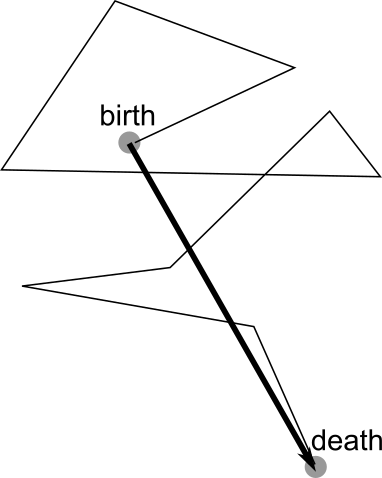
\includegraphics[scale=0.46] {figures/diffusion_length.png}}\protect
\caption{\label{fig:diffusionlength} \footnotesize{Illustration of the diffusion length.}}
\end{figure} 

\subsubsection{Solution to the diffusion equation in simple geometries}

Let us briefly solve the diffusion equation for three simple, homogeneous geometries. In D\&H you can find the derivation for other geometries as well.

\subsubsection*{1D multiplying slab}

If we rearrange the equation we arrive to the Helmholtz-equation

\begin{equation}
-\frac{\nabla^2 \Phi}{\Phi}=\frac{\frac{1}{k}\bar\nu\Sigma_f-\Sigma_a}{D}
\end{equation}

Or by introducing a new constant which depends on the materials of the reactor.

\begin{equation}
\nabla^2 \Phi+B_m^2\Phi=0
\end{equation}

Our trial solution is $\Phi(x)=A\cos Bx+C\sin Ex$. We know that the flux is symmetric, so  $d\Phi/dx|_{x=0}=0$, which leaves the cosine term. Let's substitute that to the original equation

\begin{equation}
-\frac{-AB^2cosBx}{AcosBx}=B^2=\frac{\frac{1}{k}\bar\nu\Sigma_f-\Sigma_a}{D}
\end{equation}

Clearly now we have used a $B^2$ which only depends on the geometry. Let's call it $B_g^2$, the geometry buckling factor. We can determine it from the boundary condition. Let's consider that the flux disappears at edges of the slab at $x=a$ and $x=-a$ (so the size of the reactor is $2a$)

\[
B_ga=\frac{\pi}{2} \rightarrow B_g=\frac{\pi}{2a}
\]

Of course, at the edge of the reactor the flux should not become zero if the slab is surrounded with vacuum as this is highlighted in Figure \ref{fig:boundary} A more meaningful boundary condition could be introduced through the partial currents. From Fick's law we could derive (see D\&H)

\begin{figure}[ht!]
\protect \centering{
\includegraphics[scale=0.46] {figures/04-vacuumboundaries.png}}\protect
\caption{\label{fig:boundary} \footnotesize{Vacuum boundaries in transport and diffusion theory. One can observe that we need to "extrapolate" the boundary for diffusion.}}
\end{figure} 


\[
J_x^\pm=\frac{1}{4}\Phi\mp\frac{1}{2}D\frac{d}{dx}\Phi
\]

And we know that for a vacuum boundary $J_x^-(a)=0$, from which we find that the flux should become zero at $a+2D$ (and based on transport equation even more accurate results could be obtained). This doesn't mean that the flux is physically zero at this location, since if the slab is surrounded by vacuum, the flux after the edge is going to be constant. It means that mathematically speaking if the flux would be extrapolated it should disappear at $a+2D$. In the following we will always assume "extrapolated boundaries", so we don't need to worry about this.

\begin{figure}[ht!]
\protect \centering{
\includegraphics[scale=0.46] {figures/04-slabflux.png}}\protect
\caption{\label{fig:multislab} \footnotesize{Mathematically correct solutions to the diffusion equation in a slab. $n=0$ is the fundamental mode.}}
\end{figure} 

Note that the Helmoltz equation produces valid solutions at $B_{g,n}a=\frac{\pi}{2}+n\pi$, so $B_{g,n}=\frac{(2n+1)\pi}{2a}$. However those will not be physical, so we keep the $n=0$ fundamental mode, as shown in Figure \ref{fig:multislab}, and for this course we don't care about the other modes.

For a critical reactor $k=1$, the constant $B_m^2$ becomes

$$B_m^2=\frac{\bar\nu\Sigma_f-\Sigma_a}{D}$$

\noindent and as mentioned earlier it only depends on the materials of the reactor. Therefore, we will call it the material buckling factor. It is clear that the condition of criticality is

\begin{equation}
B_g^2=B_m^2
\end{equation}

But it is also apparent, that in case we know the the material and the geometry buckling, we can figure out the $k$:

\begin{equation}
k=\frac{\bar\nu\Sigma_f}{DB_g^2+\Sigma_a}=\frac{\text{gains}}{\text{losses}}
\end{equation}

\noindent and this results is aligned with our previous, intuitive definition of the multiplication factor, since it is a ratio of the gains and losses of neutrons.

We can use this result to perform some basic investigations. What happens if

\begin{itemize}
\item we introduce more absorber and increase $\Sigma_a$? Then $k$ goes down.
\item we increase the size of the reactor? Then $B_g$ decreases, thus $k$ increases. 
\item we increase the temperature $T$? This is a bit more complicated question, in general we can say that the density goes down, so the number density goes down, so the macroscopic cross sections decrease. Reactor might expand, although usually, this will play only a small role. The diffusion coefficient $D$ increases (since in the denominator, the macroscopic cross sections go down): the atoms are more spread out, so neutrons can move around more easily. But as a summary, we cannot answer the question, since it depends on the exact composition of materials. 
\end{itemize}

One might ask also, where is the power in these solutions? We see that the constant describing the magnitude of the flux $A$ disappeared. Indeed, criticality doesn't depend on the power. That is just a normalization factor. We can have even (almost) zero power reactors (few watts). We can obtain the normalization factor $A$ from the power:

\begin{equation}
P=\int_V dr^3 w_f\Sigma_f\phi(r)
\end{equation}

\noindent where $w_f$ is the useful energy released in fission.

\subsubsection*{2D Cylindric reactor}

Let's assume that the flux is symmetric in $\varphi$, then the Laplace operator becomes


\[
\frac{1}{r}\frac{\partial}{\partial r}(r\frac{\partial}{\partial r})+\frac{\partial^2}{\partial z^2}
\]

Then, we will separate the variables:

\[
\Phi(r,z)=R(r)Z(z)
\]

\noindent after substituting these in the diffusion equation we arrive to

\[
Z(z)\frac{1}{r}\frac{\partial}{\partial r}(r\frac{\partial}{\partial r}R(r))+R(r)\frac{\partial^2}{\partial z^2}Z(z)=-B^2\Phi(r,z)
\]

\noindent where we can divide by $\Phi(r,z)$:

\[
\frac{1}{R(r)}\frac{1}{r}\frac{\partial}{\partial r}(r\frac{\partial}{\partial r}R(r))+\frac{1}{Z(z)}\frac{\partial^2}{\partial z^2}Z(z)=-B^2
\]

\noindent where we obtain the sum of some function $f(r)$ and $g(z)$, which is constant for all r and z. This is only possible if the two terms are also constant:


\[
\frac{1}{R(r)}\frac{1}{r}\frac{\partial}{\partial r}(r\frac{\partial}{\partial r}R(r))=-B_r^2
\]

\noindent and

\[
\frac{1}{Z(z)}\frac{\partial^2}{\partial z^2}Z(z)=-B_z^2
\]

\noindent and with that

\[
B_r^2+B_z^2=B^2
\]

The equation for the the axial dimension is exactly what we just had for the 1D slab, and in the general solution with the same thinking we can keep only the cosine 

\[
Z(z)=c_1\cos B_zz
\].  

\noindent and by considering that the height of the reactor is $H$ (extrapolated), we arrive to

\[
Z(z)=c_1cos(\frac{\pi}{H}z)
\]

For the radial dimension we need to consult our math books, and find that the function which could fulfill this equation is the Bessel function $J_0(B_rr)$. In fact, similarly as before here also the first and second kind Bessel functions would be solutions, but we drop the second kind to get positive values at $r=0$ as it is shown in Figure \ref{fig:cylinder}.

\[
R(r)=c_2J_0(\frac{2.405}{R}r)
\]

\noindent and with that the final solution is

\[
\Phi(r,z)=c\cos(\frac{\pi}{H}z)J_0(\frac{2.405}{R}r)
\]

\begin{figure}[ht!]
\protect \centering{
\includegraphics[scale=0.42] {figures/04-besselfunction.png} \includegraphics[scale=0.42] {figures/04-cylinderradialflux.png}}\protect
\caption{\label{fig:cylinder} \footnotesize{Illustration of the Bessel-functions and the radial flux profile of a cylinder.}}
\end{figure} 

\subsubsection*{1D non-multiplying slab}

Let us review a case when the material is not multiplying. Then we can obtain a steady case only if there is a source placed in the geometry. Consider a slab, with a planar source placed at the center. The diffusion equation reduces to the one-dimensional form

$$\frac{d^2\phi}{dx^2}-\frac{1}{L^2}\phi=-\frac{S(x)}{D}=-\frac{S_0}{D}\delta(x)$$

where the diffusion length $L=\sqrt{D/\Sigma_a}$ is introduced. Note that in case $x\neq 0$, the equation is even simpler:

$$\frac{d^2\phi}{dx^2}-\frac{1}{L^2}\phi=0$$

We will try to solve this homogeneous equation first, and then use some boundary conditions to get the generic solution.

One boundary condition will be

$$-D\frac{d\phi}{dx}\rvert_{+\epsilon}+D\frac{d\phi}{dx}\rvert_{-\epsilon}=J_x(0^+)-J_x(0^-)=S_0$$

and due to the symmetry of the geometry

$$J_x(0^+)=-J_x(0^-)=J(0)$$

thus the first boundary condition is

$$\mathrm{lim}_{x\rightarrow 0^+} -D\frac{d\phi}{dx}=\frac{S_0}{2}$$

\noindent thus the net current at the origin at either side must be half of the source strength.

Since we have a second order derivative we need and other boundary condition as well: we will use the condition of finite flux as $x\rightarrow \infty$:

$$\mathrm{lim}_{x\rightarrow \infty} \phi(x) < \infty$$

We solve for the positive side, and then infer symmetry for the negative side. The general solution is

$$\phi(x)=A\cdot\exp\Big(-\frac{x}{L}\Big)+B\cdot\exp\Big(\frac{x}{L}\Big)$$

\noindent where due to the second BC $B=0$. And due to the first BC

$$\mathrm{lim}_{x\rightarrow 0^+} -D\Bigg(-\frac{A}{L}\cdot\exp\Big(-\frac{x}{L}\Big)\Bigg)=\frac{AD}{L}=\frac{S_0}{2} \rightarrow A=\frac{S_0L}{2D}$$

\noindent thus the solution is (illustrated in Fig. \ref{fig:nonmultislab}).

$$\phi(x)=\frac{S_0L}{2D}\cdot\exp\Big(-\frac{|x|}{L}\Big)$$


\begin{figure}[ht!]
\protect \centering{
\includegraphics[scale=0.46] {figures/04-nonmultislab.png}}\protect
\caption{\label{fig:nonmultislab} \footnotesize{Solution to the flux in a nonmultiplying slab.}}
\end{figure} 

\subsection{Reflected geometries}

In practice the reactor is of course not surrounded with vacuum, but typically with some material which can scatter neutrons. This can mean, that the reactor core is surrounded with water, but in fast reactors often the core is surrounded with so called reflector assemblies (since the coolant would not reflect neutrons). The main reason of doing so is to reduce the leakage of neutrons.

One could derive the flux shape for a reflected geometry. We will omit the derivation in the notes (see D\&H p211), just highlight that the criticality condition $B_g^2=B_m^2$ does not hold anymore. The flux shape is shown in Fig. \ref{fig:reflected} (top), the drop of the flux inside the reflector region will depend on the properties of the material. In case the absorption cross section of the material is high the flux quickly goes to zero (of course in that case we do not talk about a reflector anymore, rather an absorber or shield. 

\begin{figure}[ht!]
\protect \centering{
\includegraphics[scale=0.46] {figures/04-reflectedslab_Diffusion.png} \includegraphics[scale=0.46] {figures/04-reflectedslab_MC.png}}\protect
\caption{\label{fig:reflected} \footnotesize{Spatial distribution of the neutron flux in a reflected slab. Top 1-group diffusion theory. Bottom Monte Carlo particle transport results.}}
\end{figure} 

However, this is a geometry for which our academic tool, the 1-group method gives a rather bad approximation. Namely, that reflected geometries besides reducing leakage also serve to flatten the flux and the power distribution. As a result of this one could observe a peaking of the thermal flux close to the boundary between the core and the reflector as shown in the bottom of Figure \ref{fig:reflected}. However, one needs to apply at least 2-group theory to analyze this effect.

Since reflectors reduce leakage, the fissile core can have a smaller size to achieve criticality. This is called the reflector savings

\begin{equation}
\delta = a_{bare}-a_{reflector}
\end{equation}

\noindent which can be derived as a function of the reflector savings (D\&H p214). Figure \ref{fig:reflectorsavings} illustrates this. The figure indicates how much the critical size can be decreased when the reflector is added. As one would expect intuitively, the function saturates (at around $b=3L_r$), which means that after a certain reflector thickness the critical size of the core cannot be reduced, since neutrons will not reach to and scattered back from such a far distance.

\begin{figure}[ht!]
\protect \centering{
\includegraphics[scale=0.46] {figures/04-reflectorsavings.png}}\protect
\caption{\label{fig:reflectorsavings} \footnotesize{Reflector savings.}}
\end{figure} 

\subsection{2 and Multi group diffusion}

As we saw from the reflected geometry, the 1-group diffusion theory cannot adequately capture all physical phenomena, thus in practice at least 2, but often more groups are used. Within this course we do not intend to solve the 2-group problem analytically, or to implement multi-group numerical solvers, we will only draft the idea behind multigroup methods by developing a 2-group equation.

In 2-group theory the energy boundaries are selected so that there is no upscattering from the thermal to the fast group. The typical boundaries are $E_2=0$, $E_1=1 eV$, $E_0=10 MeV$. In such group structure, we can assume that all the fission event contribute as a source only to the fast group, therefore $\chi_t=0$ and $\chi_f=1$.

Let us summarize the gain and loss term in each of the groups (index $f$ refers to the fast group, and $t$ refers to the thermal group; when double indexes are encountered such as in $\Sigma_{f,t}$, the first term refers to the physical process, such as fission in this example, and the second to the energy group, such as thermal in this example).


\begin{tabular}{c | c | c}
group & Gains & Losses \\
\hline
fast & $\frac{1}{k}\nu_t\Sigma_{f,t}\Phi_t+\frac{1}{k}\nu_f\Sigma_{f,f}\Phi_f$ & $\Sigma_{a,f}\Phi_f + \Sigma_{s,f\rightarrow t}\Phi_f + D_fB_g^2\Phi_f$  \\
\hline
thermal & $\Sigma_{s,f\rightarrow t}\Phi_f$ & $\Sigma_{a,t}\Phi_t  + D_tB_g^2\Phi_t$ 
\end{tabular}

The sources of neutrons in the fast group are both from thermal and fast fission. The sources is of neutrons in the thermal group are only from downscattering from the fast group. Both energy groups lose neutrons due to absorption and leakage, however the downscattering appears as a loss in the fast group.

With these source and loss terms it is possible to develop a coupled set of balance equation for each groups.

\begin{equation}
\frac{1}{k}\nu_t\Sigma_{f,t}\Phi_t+\frac{1}{k}\nu_f\Sigma_{f,f}\Phi_f=\Sigma_{a,f}\Phi_f + \Sigma_{s,f\rightarrow t}\Phi_f + D_fB_g^2\Phi_f 
\end{equation}

\begin{equation*}
\Sigma_{s,f\rightarrow t}\Phi_f = \Sigma_{a,t}\Phi_t  + D_tB_g^2\Phi_t
\end{equation*}


By rearranging the second, we get an expression for the thermal flux

\begin{equation}
\Phi_t=\frac{\Sigma_{s,f\rightarrow t}\Phi_f}{\Sigma_{a,t}  + D_tB_g^2}
\end{equation}

\noindent which can be substituted into the first one

\begin{equation}
\frac{1}{k}\nu_t\Sigma_{f,t}\frac{\Sigma_{s,f\rightarrow t}\Phi_f}{\Sigma_{a,t}  + D_tB_g^2}+\frac{1}{k}\nu_f\Sigma_{f,f}\Phi_f=\Sigma_{a,f}\Phi_f + \Sigma_{s,f\rightarrow t}\Phi_f + D_fB_g^2\Phi_f
\end{equation}

\noindent Then after dividing by $\Phi_f$, one can rearrange for $k$.

\begin{equation}
k=\frac{\nu_t\Sigma_{f,t}\frac{\Sigma_{s,f\rightarrow t}}{\Sigma_{a,t}  + D_tB_g^2}+\nu_f\Sigma_{f,f}}{\Sigma_{a,f} + \Sigma_{s,f\rightarrow t} + D_fB_g^2}=\frac{\text{gains}}{\text{losses}}
\end{equation}

And notice that similarly as before, we could identify the terms as gains and losses.


\begin{figure}[ht!]
\protect \centering{
\includegraphics[scale=0.46] {figures/04-controlrod.png}}\protect
\caption{\label{fig:controlrod} \footnotesize{Change in the axial flux shape due to control rod insertion.}}
\end{figure}

\subsection{Control rods}

It is noteworthy to mention that certain elements in the reactor, such as control rods, can drastically change the spatial distribution of neutrons in the core, and also have an impact on the multiplication factor of the system. Figure \ref{fig:controlrod} illustrates the influence of a control rod insertion on the axial flux. We can see that the peak of the flux will shift to deeper regions of the core. The impact of the rod on the reactivity 

\[
\rho=\frac{k-1}{k}
\]

\noindent can be given by the control rod worth, which describes the change in the k-effective $\Delta k$ due to the insertion of the control rod.  

\subsection{Calculation scheme}

As a final note to our discussion on neutron transport, it is important to highlight that in this chapter we have barely scratched the surface. There is no numerical solution to the transport problem which can be applied directly at each levels of the reactor core besides Monte Carlo methods. Therefore the problem is typically split into tasks as illustrated with an oversimplified scheme in Figure \ref{fig:calculationscheme}. First the continuous cross section data is processed to obtain group-wise data. Then this is used to tackle the slowing down and thermalization problem at a pin or lattice level to obtain few group cross sections. Finally that is used in core level diffusion solvers. There can be of course other task to include depending the application, such as depletion calculations, or transient calculations, which are the topics of the following chapters.

\begin{figure}[ht!]
\protect \centering{
\includegraphics[scale=0.46] {figures/calculationscheme.png}}\protect
\caption{\label{fig:calculationscheme} \footnotesize{Schematic illustration of the reactor calculation process.}}
\end{figure} 


%\end{document}


%\documentclass[12pt]{article}
%\usepackage{amsmath}
%\usepackage{graphicx, color}
%\usepackage{amssymb}
%\usepackage{listings} %source code listing
%\usepackage{multirow}
%\usepackage[version=2]{mhchem}
%\usepackage{subfig}
%\usepackage{hyperref}
%\usepackage{units}
%\usepackage{gensymb}
%\usepackage{adjustbox}
%\usepackage{listings}
%\usepackage{color}
%\usepackage{tcolorbox}
% 
%\definecolor{codegreen}{rgb}{0,0.6,0}
%\definecolor{codegray}{rgb}{0.5,0.5,0.5}
%\definecolor{codepurple}{rgb}{0.58,0,0.82}
%\definecolor{backcolour}{rgb}{0.95,0.95,0.92}
%
%\newcommand{\specialcell}[2][c]{%
%  \begin{tabular}[#1]{@{}c@{}}#2\end{tabular}}
% 
%
%
%\title{Reactor physics with Python \\ Lecture Notes}
%
%
%\author{Zs.~Elter. E. Branger, M. Preston \\ Uppsala University \\
%        Division of Applied Nuclear Physics}%\corref{cja}}
%%
%\date{2021.}
%\begin{document}

\section{Time dependence in reactor physics}

Up to now we have considered the reactor to be at a steady state, when the number of neutrons does not change in time. This is however not always the case: even during normal reactor operation the power might need to be adjusted, which requires the momentary increase or decrease of the multiplication factor of the core, which then results in the increase or decrease of the neutron population. This chapter first discusses the the time-behavior of reactors with the help of the point kinetic model.

Then we continue our discussions with subcritical systems driven by a neutron source. Although such systems are in fact steady, but due to the low number of neutrons, the statistical fluctuations of the neutron population and the time correlation of single neutron detections due to the stochastic nature of neutron transport become relevant. 

In a nuclear reactor due to fission the concentration of fissile nuclei is decreasing, while the concentration of fission products is increasing. These changes are not relevant on short time scales, thus in our previous discussions it was not necessary to take them into account. Nevertheless, the due to this change the macroscopic cross sections $\Sigma(\mathbf{r},E,t)$ are in fact time dependent. Therefore our last subject of time-dependent processes will be the depletion of fuel.

\subsection{Nuclear Reactor Kinetics}
Up to this point, we have only considered the case of a critical reactor, i. e. a system in which the neutron production in fission is just right to keep the chain reaction going. The neutron diffusion equation may be solved for such a system to describe the neutron production, transport and absorption in the core, as well as possible leakage of neutrons from the core. The neutron flux in such a system of course depends on both space and time --- neutrons are after all particles moving throughout the core, inducing fission at various locations. Nonetheless, if we assume a critical reactor, the neutron production balances the absorption and fission such that there is no \emph{overall} change in the neutron population in the core. That is, the neutron flux in this assumed critical core is \emph{time-independent}. In this chapter, we will make a step towards a more realistic description of the time-dependent system that a nuclear reactor really is. To do that, we study \emph{reactor kinetics}.

Studying the time-dependence of the reactor behaviour is important for a number of reasons. The reactor core is not an isolated system, but is for example connected to turbines generating electricity. Should the load on these turbines be perturbed, the steam demand will also be altered, affecting for instance the temperature or pressure in the reactor vessel. In a water-moderated core, these parameters will have an impact on the moderation rate and therefore also on the energy distribution of neutrons in the core. Because the cross sections vary with neutron energy, there will be an impact on the neutron production and loss in the core --- the system will be perturbed from its critical state. Another effect is the long-term change in fuel composition: after more and more fissions in the fuel, its composition will change in a way such that the neutron balance that held true in the initial critical core no longer does. Effects such as these require the operator to take action to keep the system critical. As we shall see in this chapter, the time dependence of the system is absolutely vital for such control to be possible.

In subsequent chapters, we will return to some of the more concrete examples of time dependence in a nuclear reactor: sources of feedback, depletion and poisoning. In this chapter, the focus will be on extending the neutron diffusion equation to a time dependent system. It is first important to point out one key assumption that will hold throughout this chapter: that the \emph{spatial} dependence of the neutron flux is fixed at the fundamental mode. That is, we assume that localised fluctuations in the neutron flux will die away rather quickly, yielding a fixed spatial distribution of the neutrons. This assumption is referred to as the \emph{point-kinetics approximation} (although the spatial dependence of the flux is not described as a point, but rather a fixed distribution). We then assume that any time dependence in the flux will simply scale the neutron flux up or down while keeping the spatial shape fixed.

\subsubsection{Reactor with only prompt neutrons}
\label{sec:prompt_neutrons}
In the treatment of the neutron diffusion equation up to this point, it has been assumed that the neutron source (i. e. the number of neutrons produced per second per volume) from fission in the reactor is given by:
\begin{equation}
	S_\text{f}(\vec{r}, t) = \overline{\nu} \overline{\Sigma}_\text{f}\overline{v}n(\vec{r}, t),
	\label{eq:prompt_source}
\end{equation}
where $\overline{\nu}$ is the average neutron multiplicity (i. e. the average number of \emph{prompt} neutrons released in the fission event), $\overline{\Sigma}_\text{f}$ is the average macroscopic fission cross section, $\overline{v}$ is the average neutron velocity and $n(\vec{r}, t)$ is the space- and time-dependent neutron density. The neutron multiplicity, macroscopic cross section and neutron velocity have been averaged over the nuclei in the fuel as well as the neutron energy, yielding a one-speed description of the source. Here, I have emphasised the word \emph{prompt} because it is important for the purpose of this chapter.

By recognising that the one-speed neutron flux $\overline{\phi}(\vec{r}, t) = \overline{v}n(\vec{r}, t)$, Eq. \ref{eq:prompt_source} may be incorporated into the neutron diffusion equation (we now drop the overline notation denoting one-speed averaged, since we will be using those throughout the chapter):
\begin{equation}
	\frac{1}{v}\frac{\partial \phi}{\partial t} = \nu \Sigma_\text{f}\phi(\vec{r}, t) + \nabla \cdot D\nabla \phi(\vec{r}, t) - \Sigma_\text{a}\phi(\vec{r}, t),
	\label{eq:diffusion_eq}
\end{equation}
where $D$ is the diffusion coefficient and $\Sigma_\text{a}$ is the one-speed macroscopic absorption cross section. Here, we should make an important note: of course the above equation can be modified if there are additional sources of neutrons in the system (such as when starting up the system), or when considering non-multiplying materials. Adding and/or removing the corresponding terms in the above equation would result in different sets of differential equations for the neutron population, which may be solved. In this chapter, we will however focus on the results for the system described above. Now, if we come back to the assumption behind the point kinetics approximation, the spatial dependence of the neutron flux in the core is fixed and may be written $\psi_1(\vec{r})$ (the subscript denotes that this is the fundamental spatial mode of the flux). As stated earlier, the time dependence of the flux lies in a time-dependent scaling of this flux. That is, the flux $\phi(\vec{r}, t)$ is written as a product of a time-dependent part and a space-dependent part:
\begin{equation}
	\phi(\vec{r}, t) = v n(t) \psi_1(\vec{r}),
	\label{eq:neutron_flux_time_space}
\end{equation}
where we have used the definition of neutron flux as the product of the neutron velocity and the neutron density. Inserting this into the diffusion equation Eq. \ref{eq:diffusion_eq} yields:
\begin{equation}
	\frac{1}{v} v \psi_1(\vec{r})\frac{\partial n}{\partial t} = \nu \Sigma_\text{f}v n(t) \psi_1(\vec{r}) + v n(t) \nabla \cdot D\nabla \psi_1(\vec{r}) - \Sigma_\text{a}v n(t) \psi_1(\vec{r}).
	\label{eq:diffusion_eq_expanded1}
\end{equation}
Because the time- and space-dependences are nicely separated, $\nabla \cdot D\nabla \psi_1 = D\nabla^2 \psi_1$. This is a measure of the curvature of the spatial dependence of the flux, and because we are here only concerned with the fundamental spatial mode, this can be rewritten in terms of the geometric buckling $B_g^2 \equiv B_1^2$:
\begin{equation}
	B_1^2 \equiv B_g^2 = -\frac{1}{\psi_1}\nabla^2\psi_1.				% from Eq. 5-208 in D&H
\end{equation}
Inserting this into Eq. \ref{eq:diffusion_eq_expanded1} yields:
\begin{equation}
	\frac{d n}{d t} = \nu \Sigma_\text{f}v n(t) - v n(t) D B_g^2 - \Sigma_\text{a}v n(t) = (\nu \Sigma_\text{f} - D B_g^2 - \Sigma_\text{a})v n(t).
	\label{eq:diffusion_eq_expanded2}
\end{equation}
Introducing three new variables $L$, $l$ and $k$:
\begin{equation}
	L \equiv \text{Diffusion length} \equiv \sqrt{\frac{D}{\Sigma_\text{a}}}
\end{equation}
\begin{equation}
	l \equiv \text{Mean neutron lifetime} \equiv \frac{1}{v \Sigma_\text{a}(1 + L^2 B_g^2)}
\end{equation}
\begin{equation}
	k \equiv \text{Multiplication factor} \equiv \frac{\nu \Sigma_\text{f}/\Sigma_\text{a}}{1 + L^2 B_g^2}
\end{equation}
The diffusion length $L$ can be viewed as a measure of how far (on average) a neutron in a system travels between it's birth and it's absorption. The mean neutron lifetime $l$ can be viewed as the time (on average) between the birth of a neutron and it's absorption. In a thermal reactor, $l \simeq 10^{-4}$ seconds, whereas in a fast reactor $l \simeq 10^{-7}$ seconds [L\&B page 332] Finally, the multiplication factor $k$ is the number of neutrons produced in fission divided by the number of neutrons lost through absorption or leakage. It is worth noting that $k = k_\infty/(1 + L^2 B_g^2)$, where $k_\infty$ is the multiplication factor in an infinite core and the denominator corrects for leakage from the boundary of the core. Using these relationships together with Eq. \ref{eq:diffusion_eq_expanded1} yields
\begin{equation}
	\frac{dn}{dt} = \left( \frac{k - 1}{l} \right) n(t),
	\label{eq:diffusion_eq_expanded3}
\end{equation}
which is a differential equation with the following solution for $n(t)$:
\begin{equation}
	n(t) = n_0 \exp \left[\left(\frac{k-1}{l}\right)t\right] = n_0 \exp[-t/T].
	\label{eq:diffusion_eq_expanded4}
\end{equation}
That is, the time-dependence of the neutron flux in the core is characterised by an exponential with a time constant $1/\left(\frac{k-1}{l}\right) \equiv T$. This time constant $T$ is called the \emph{reactor period}. This constant characterises the time scale on which the neutron flux in the reactor changes given a certain deviation of $k$ from one. That is, if the system leaves its critical state (at $k=1$), the time scale at which the resulting change of flux (and correspondingly, power) happens is characterised by the time $T$. A small $T$ means that even a small deviation of $k$ from one will result in a rapid change in the neutron flux (and core power). A large $T$ on the other hand means that a small deviation of $k$ from one will result in slow changes in the flux (and core power). Combining this with Eq. \ref{eq:neutron_flux_time_space} yields a final expression for the neutron flux in the core:
\begin{equation}
	\phi(\vec{r}, t) = v n_0 \exp [t/T] \psi_1(\vec{r}).
	%\label{eq:neutron_flux_time_space}
\end{equation}
Here, it is again worth to note that the space-dependent factor $\psi_1(\vec{r})$ determines the \emph{shape} of the flux, and the time-dependent factor determines the \emph{amplitude} of the flux. We will for the rest of this chapter only focus on the time-dependent part, which gives us the overall neutron population/neutron flux/power of the system. Because the reactor period $T$ gives us a measure of the time available to control the reactor, it is now interesting to determine $T$ for an example reactor using the equations above:
\begin{tcolorbox}
Exercise

Consider a thermal nuclear reactor which is critical at time $t = 0$. If the neutron multiplication factor $k$ is increased from 1 to 1.001, what is the increase in the neutron flux?

	In a thermal reactor, the mean neutron lifetime $l \simeq 10^{-4}$ seconds (as stated above). Using the expression for the reactor period $T$ defined above:
	\[
		T = \frac{l}{k-1} = \frac{10^{-4}}{1.001 - 1} = 0.1\text{ seconds}
	\]

	Using this value in Eq. \ref{eq:diffusion_eq_expanded4} yields a relative increase in the neutron population $n(t)$ after the change in $k$:
	\[
		\frac{n(t)}{n_0} = \exp[t/0.1]
	\]

	Since the neutron flux is proportional to the neutron population, this ratio also gives the relative increase in the neutron flux. Should this (small) increase in $k$ happen over a time of 1 second, the neutron flux (and therefore also the power of the reactor) would increase by a factor of 22,000! Clearly this is a very large increase in power even for a small perturbation of the multiplicity factor $k$. You can yourself perform the same calculation for a fast reactor with a mean neutron lifetime of $l \simeq 10^{-7}$ seconds.
\end{tcolorbox}

As you see in the above exercise, a system such as the one we have described so far will be \emph{very} difficult to control, with large changes in neutron flux and power even for small perturbations of the system. Luckily, there is a factor which we so far have not accounted for, which \emph{does} make the system controllable: delayed neutrons. As the name suggests, these are neutrons that for some reason are delayed in time. It is important to note that this delay refers to the generation of neutrons in the reactor, and that we have so far not included any time-dependence in the fission neutron source. That is, when describing the neutron diffusion equation, we have assumed neutrons to originate in fission according to the source term $\nu \Sigma_\text{f}\phi(\vec{r}, t)$ (see Eqs. \ref{eq:prompt_source} and \ref{eq:diffusion_eq}). In this source term, there is no reference to any time distribution of the generated neutrons --- all of them are promptly produced in the moment of fission. However, this is not the whole truth, and as we shall see this has very important consequences for the operation of nuclear reactors.

\subsubsection{Reactor with prompt and delayed neutrons}
As you may remember from our discussions of radioactive decay, an atomic nucleus may decay through several mechanisms such as $\alpha$ decay, $\beta$ decay and fission. A decay mechanism which is relatively rare, but nonetheless very important for nuclear reactor operations, is \emph{neutron emission}. Occurring in some neutron-rich nuclei, neutron emission means that an excited nucleus emits a neutron to form a nucleus with one fewer neutrons. In the context of reactor operations, it is more relevant to talk about $\beta$-delayed neutron emission. Since neutron emission requires a neutron-rich nuclei, we are talking about $\beta^-$ decays. Consider a beta-unstable nucleus $(Z, N)$ being produced as a fission product in the reactor. This nucleus, which we from now on call the \emph{precursor} may decay through $\beta^-$ decay with a certain half life. After the beta decay, an unstable daughter nucleus $(Z+1, N-1)$ is formed. Some of these daughter nuclei may then decay by neutron emission --- a process which occurs directly after the $\beta^-$ decay. Therefore, the time scale is defined by the half life of the precursor $\beta^-$ decay.

To date, a large number of delayed-neutron precursors have been discovered [e.g. https://doi.org/10.1016/j.nds.2020.09.001]. In order to complement our prompt-neutron source with these delayed neutrons, we could therefore proceed to calculate the emission rate of each source of delayed neutrons. After all, different precursors will have different $\beta^-$ half lives, and therefore introduce different time dependencies in the overall delayed-neutron source. However, there are at least two problems with this approach: i) there is a very large number of precursors and ii) not all precursors are known. Instead, what is typically done is ``lumping together'' various delayed-neutron precursors that have similar half-lives, after which an ``average'' half life is determined. The different precursors will of course have different fission yields (i. e. be produced to different extents in the reactor), and this is taken into account by an ``effective fraction'' $\beta$ (the number of emitted delayed neutrons relative to the total neutron emission from fission). One should remember that fission yields will depend on the fuel composition (i.e. which fissioning nuclei are present in the fuel) and the energies of the neutrons inducing fission, so the effective yield will depend on the fuel composition and neutron energy in the reactor. Table \ref{tab:delayed_n} lists the properties of six-group (i. e. the precursors have been ``lumped together'' based on six characteristic half lives) delayed neutrons in $^{235}$U. It is worth noting that the six-group representation is not the only possibility --- for instance eight-group delayed neutrons may be used [https://arxiv.org/pdf/2102.01165.pdf].
\begin{table}
        \centering
	\caption{Six-group delayed neutrons from $^{235}$U. The total delayed-neutron fraction $\beta = \sum \beta_i = 0.0065$ = 0.65\%. Data taken from [L\&B table 3.5]}
	\label{tab:delayed_n}
\begin{tabular}{ l l l }
	Group & Half life [s] & Fraction $\beta_i$ \\
  \hline
	1 & 55.72 & 0.000215\\
	2 & 22.72 & 0.001424\\
	3 & 6.22 & 0.001274\\
	4 & 2.30 & 0.002568\\
	5 & 0.610 & 0.000748\\
	6 & 0.230 & 0.000273\\
  \hline
\end{tabular}
\end{table}

In Table \ref{tab:delayed_n}, we note that delayed neutrons make up only approximately 0.7\% of the total neutron population in the core. This is certainly a small number, but let's consider what they contribute with to the \emph{time-dependence} of the neutron population. Again, we stress that by defining six groups of delayed neutrons, we move away from a well-defined physical meaning of those six groups. That is, each group contains contributions from various delayed-neutron precursor nuclei. Therefore, a particular group does \emph{not} represent a particular nucleus (although some nuclei may dominate in the different groups). Understanding this, we first define the precursor density $C_i$ for each delayed-neutron group. $C_i$ is the number of precursors in group $i$ per volume whose decay \emph{always} results in the emission of a delayed neutron. That is, we consider only the precursors that for sure will give us a delayed neutron (this is of course a subset of the actual number of precursors, since there may be other decay modes). The number of decays $D_i$ per second per volume of these $C_i$ precursors is given by:
\begin{equation}
	D_i(\vec{r}, t) = \lambda_i C_i(\vec{r}, t)
\end{equation}
At the same time, precursors are produced in fission. The number of produced precursors $P_i$ per second per volume is:
\begin{equation}
	P_i(\vec{r}, t) = \beta_i \nu \Sigma_\text{f} \phi(\vec{r}, t),
\end{equation}
which in many ways reminds us of the prompt-fission neutron source in Eq. \ref{eq:prompt_source}, albeit with an additional term $\beta_i$ to denote that only a fraction of all neutrons produced will be delayed. The overall rate of change in the precursor density $C_i$ is therefore given by:
\begin{equation}
	\frac{\partial C_i}{\partial t} = \beta_i \nu \Sigma_\text{f} \phi(\vec{r}, t) - \lambda_i C_i(\vec{r}, t).
	\label{eq:C_net_change}
\end{equation}

Since each decay of $C_i$ results in an emitted neutron, we may rewrite our original source term Eq. \ref{eq:prompt_source}, now including \emph{both} prompt and delayed neutrons:
\begin{equation}
	S_\text{f}(\vec{r}, t) = (1-\beta) \nu \Sigma_\text{f}\phi(\vec{r}, t) + \sum_{i=1}^6 \lambda_i C_i(\vec{r}, t),
	\label{eq:prompt_delayed_source}
\end{equation}
where $(1-\beta)$ of course is the fraction of all neutrons that are \emph{not} delayed (i. e. are prompt). We now proceed through the same steps as in Sec. \ref{sec:prompt_neutrons} to get a description of the time dependence of the neutron population, only now we include the delayed neutrons. First, we introduce the new source term (Eq. \ref{eq:prompt_delayed_source}) into the diffusion equation, yielding:
\begin{equation}
	\frac{1}{v}\frac{\partial \phi}{\partial t} = (1-\beta) \nu \Sigma_\text{f}\phi(\vec{r}, t) + \sum_{i=1}^6 \lambda_i C_i(\vec{r}, t) + \nabla \cdot D\nabla \phi(\vec{r}, t) - \Sigma_\text{a}\phi(\vec{r}, t),
	\label{eq:diffusion_eq_delayed}
\end{equation}

If we again consider our assumption that the space- and time-distribution of the neutron density (and flux) in the core may be separated into a product of a space-dependent part (determining the shape of the distribution) and a time-dependent part (determining the amplitude of the distribution), Eq. \ref{eq:diffusion_eq_delayed} yields (compare Eq. \ref{eq:diffusion_eq_expanded2}:
\begin{equation}
	\frac{d n}{d t} = (1-\beta) \nu \Sigma_\text{f} v n(t) + \sum_{i=1}^6 \lambda_i C_i(t) - v n(t) D B_g^2 - \Sigma_\text{a}v n(t).
	\label{eq:diffusion_eq_delayed_expanded2}
\end{equation}
When using the same definitions of $k$ and $l$ as earlier, we arrive at:
\begin{equation}
	\frac{dn}{dt} = \left( \frac{k(1 - \beta) - 1}{l} \right) n(t) + \sum_{i=1}^6 \lambda_i C_i(t).
	\label{eq:diffusion_eq_delayed_expanded3}
\end{equation}

If the neutron distribution throughout the core is separable in time and space, we may also do the same for the precursor densities $C_i$:
\begin{equation}
	C_i(\vec{r}, t) = C_i(t) \psi_1(\vec{r}).
\end{equation}
Inserting this into Eq. \ref{eq:C_net_change}, we end up with:
\begin{equation}
	\frac{d C_i}{d t} = \beta_i \nu \Sigma_\text{f} v n(t) - \lambda_i C_i(t) = \beta_i \frac{k}{l} n(t) - \lambda_i C_i(t).
	\label{eq:C_change}
\end{equation}

Eqs. \ref{eq:diffusion_eq_delayed_expanded3} and \ref{eq:C_change} are generalisations of our results from Sec. \ref{sec:prompt_neutrons}. They are known as the \emph{point kinetics equations}. They describe the effect of including delayed neutrons into the reactor. At this point one could think of determining the reactor period $T$ as was done for the prompt system, to see the effect of delayed neutrons. However, when we compare Eq. \ref{eq:diffusion_eq_expanded3} (the differential equation for $n(t)$ with only prompt neutrons) with Eqs. \ref{eq:diffusion_eq_delayed_expanded3} and \ref{eq:C_change}, we see that the delayed neutrons yield a system of coupled differential equations, which is more difficult to solve. We therefore need a few additional steps before we can determine the reactor period in this more realistic system. We begin by defining a parameter $\Lambda$ --- the mean neutron generation time:
\begin{equation}
	\Lambda \equiv \frac{l}{k}.
	\label{eq:Lambda_def}
\end{equation}
Because $l$ is the mean neutron lifetime (the average time between the birth and absorption of a neutron) and $k$ is the ratio between the number of neutrons produced in fission and the number of neutrons lost in absorption or leakage, $\Lambda$ is the average time between the birth of a neutron and its absorption inducing fission ($k$ is the fraction of the neutrons used for inducing fission).

We also define the \emph{reactivity} $\rho$:
\begin{equation}
	\rho(t) \equiv \frac{k(t) - 1}{k(t)},
	\label{eq:rho_def}
\end{equation}
where you'll notice the time dependence in both $\rho$ and $k$ --- we are now talking about a time-dependent system, not one which is steady state at $k = 1$. The reactivity $\rho$ is a measure of the deviation of the multiplicity factor $k$ from $k = 1$. That is, $\rho$ tells us how far from criticality the system is. It is a parameter that can, in part, be controlled by the reactor operator, for instance insertion of control rods will provide a negative reactivity insertion into the system. It is worth noting that $-\infty < \rho \leq 1$: when $\rho = 1$, $k = \infty$, when $\rho = -\infty$, $k = 0$ and when $\rho = 0$, $k = 1$. By using $\Lambda$ and $\rho$ we may re-write the point kinetics equations into a more compact form:
\begin{equation}
	\frac{dn}{dt} = \left( \frac{\rho - \beta}{\Lambda} \right) n(t) + \sum_{i=1}^6 \lambda_i C_i(t).
	\label{eq:point_kinetics1}
\end{equation}
\begin{equation}
	\frac{d C_i}{d t} = \frac{\beta_i}{\Lambda} n(t) - \lambda_i C_i(t).
	\label{eq:point_kinetics2}
\end{equation}

Before we attempt to solve the point kinetics equations, it is important to discuss their limitations. When deriving them, we have made some important assumptions:
\begin{itemize}
	\item We have not considered any dependence on neutron energy --- instead, we have always averaged over neutron energy to get the one-speed diffusion equation. In reality, nuclear cross sections depend on energy. Delayed neutrons are typically emitted with lower energies than prompt neutrons, affecting the reaction probabilities.
	\item We have assumed that the spatial shape of the neutron population is independent of time. In reality, the fuel composition will vary with time to different degrees in the core, resulting in a change in the spatial part of the flux.
	\item We have neglected the fuel composition. If the fuel for instance contains several isotopes of plutonium, each with different delayed-neutron fractions, the number of required delayed neutron groups will increase.
	\item We have neglected the effects of feedback. There are a number of factors which influence the reactivity in a core --- an increase in the reactivity will lead to an increased neutron flux, which will increase the power and thus the temperature in the core. The temperature will affect the reaction rates in the reactor, and therefore the reactivity itself.
\end{itemize}
While it is important to identify limitations such as these, it should be pointed out that the point kinetics equations can be used in a wider setting than the one based on our assumptions. The point kinetics equations may for instance be derived for a more realistic system resulting in new expressions for the parameters $\beta$, $\Lambda$ and $\rho$. The equations are therefore similar to the simplified case we have considered, motivating the use of Eqs. \ref{eq:point_kinetics1} and \ref{eq:point_kinetics2} in the context of this course. Therefore, we now proceed to solve the point kinetics equations for some important cases.

\subsubsection{Solutions to the point kinetics equations}
\subsubsection*{One effective group of delayed neutrons}
In our derivation of the point kinetics equation, we assumed six groups of delayed neutrons. To make a first attempt at actually solving these equations, we take one step back. Imagine that we lump together the six groups into one ``effective'' group of delayed neutrons. The delayed neutron fraction $\beta$ is then simply the sum over the six groups. The average decay constant (corresponding to the half life) may be determined by first determining the average lifetime $\langle t \rangle$:
\begin{equation}
	\langle t \rangle = \frac{\int_0^\infty \left( t \sum_{i=1}^6 \beta_i \lambda_i \exp[-\lambda_i t] \right) dt}{\int_0^\infty \left( \sum_{i=1}^6 \beta_i \lambda_i \exp[-\lambda_i t] \right) dt},
\end{equation}
which is a standard expected value for the variable $t$. Note that the functions averaged over are the delayed-neutron emission rates $\beta_i \lambda_i \exp[-\lambda_i t]$. Solving this equation yields an expression for $\langle t \rangle$, which is the inverse of $\langle \lambda \rangle$, the average decay constant:
\begin{equation}
	\langle \lambda \rangle = \frac{1}{\langle t \rangle} = \frac{1}{\frac{1}{\beta} \sum_{i=1}^6 \frac{\beta_i}{\lambda_i}},
\end{equation}
where $\beta$ is the sum of all $\beta_i$. Now we may write the point kinetics equations for this case, similar to Eqs. \ref{eq:point_kinetics1} and \ref{eq:point_kinetics2}:
\begin{equation}
	\frac{dn}{dt} = \left( \frac{\rho - \beta}{\Lambda} \right) n(t) + \langle \lambda \rangle C(t).
	\label{eq:point_kinetics1_one_group}
\end{equation}
\begin{equation}
	\frac{d C}{d t} = \frac{\beta}{\Lambda} n(t) - \langle \lambda \rangle C(t).
	\label{eq:point_kinetics2_one_group}
\end{equation}

We now consider the case where the reactor is in a steady state prior to $t = 0$. That is, it is critical and at $t = 0$ the reactivity changes. Given the steady state condition (i. e. all time-derivatives become zero) at $t < 0$ and the two equations above:
\begin{equation}
	\left( \frac{\rho(t < 0) - \beta}{\Lambda} \right) n(t < 0) + \langle \lambda \rangle C(t < 0) = 0
\end{equation}
\begin{equation}
	\frac{\beta}{\Lambda} n(t < 0) - \langle \lambda \rangle C(t < 0) = 0.
\end{equation}
Considering that $\rho(t < 0) = 0$ (i. e. the reactor is critical), we may combine these two equations to yield initial conditions for $n$ and $C$:
\begin{equation}
	2\langle \lambda \rangle C(t < 0) = \left[ \frac{\beta}{\Lambda} - \frac{\rho}{\Lambda} + \frac{\beta}{\Lambda} \right]n(t < 0) \Rightarrow C(t < 0) = \frac{\beta}{\lambda \Lambda} n(t < 0)
\end{equation}

The resulting initial conditions are that at $t = 0$, the neutron population is unchanged, giving $n_0 \equiv n(t = 0) = n(t < 0)$. The same thing goes for the precursor density, so $C_0 \equiv C(t = 0) = C(t < 0)$. We may postulate exponential solutions for $n(t)$ and $C(t)$:
\begin{equation}
	n(t) = A \exp[st]
\end{equation}
\begin{equation}
	C(t) = B \exp[st]
\end{equation}
$A$ and $B$ are yet to be determined. If we insert these equations into Eqs. \ref{eq:point_kinetics1_one_group} and \ref{eq:point_kinetics2_one_group}, we get:
\begin{equation}
	sA = \left[ \frac{\rho - \beta}{\Lambda} \right] A + \lambda B
\end{equation}
\begin{equation}
	sB = \frac{\beta}{\Lambda} A - \lambda B
\end{equation}
We can eliminate $A$ and $B$ by combining these equations. The result is:
\begin{equation}
	\left[ s - \left( \frac{\rho - \beta}{\Lambda} \right) \right] [s+\lambda] - \frac{\lambda \beta}{\Lambda} = 0,
	\label{eq:s_quadratic1}
\end{equation}
which is the same as
\begin{equation}
	\Lambda s^2 +(\lambda \Lambda + \beta - \rho ) -\rho\lambda = 0,
	\label{eq:s_quadratic2}
\end{equation}
which we recognise as a quadratic equation in terms of $s$. The solutions for $s$ follow the same pattern as any quadratic equation:
\begin{equation}
	s_{1, 2} = \frac{-(\lambda \Lambda + \beta - \rho) \pm \sqrt{(\lambda \Lambda + \beta - \rho)^2 + 4\Lambda\lambda\rho}}{2\Lambda}
	\label{eq:s_solutions}
\end{equation}
Since there are two roots for $s$, the general expressions for $n$ and $C$ are:
\begin{equation}
	n(t) = A_1 \exp[s_1t] + A_2 \exp[s_2t]
\end{equation}
\begin{equation}
	C(t) = B_1 \exp[s_1t] + B_2 \exp[s_2t]
\end{equation}

Although we haven't determined the values of $A_1$, $A_2$, $B_1$ and $B_2$, we may still examine some example cases by inserting different values of $\rho$ into Eq. \ref{eq:s_solutions}:
\begin{itemize}
	\item For a critical system ($\rho = 0$), $s_1 = 0$ and $s_2 = -\left(\lambda + \frac{\beta}{\Lambda}\right)$. The neutron and precursor densities will change as:
		\[
			n(t) = A_1 + A_2 \exp \left[-\left(\lambda + \frac{\beta}{\Lambda}\right)t\right]
		\]
		\[
			C(t) = B_1 + B_2 \exp \left[-\left(\lambda + \frac{\beta}{\Lambda}\right)t\right]
		\]
		That is, as $t \rightarrow \infty$, they will approach constant values.
	\item For a subcritical system ($\rho < 0$), $s_1 < 0$ and $s_2 < 0$. The neutron and precursor densities will both be sums of negative exponentials. That is, as $t \rightarrow \infty$, they will approach $n = 0$ and $C = 0$. The system will shut down.
	\item For a supercritical system ($\rho > 0$), $s_1 > 0$ and $s_2 < 0$. The neutron and precursor densities will both be sums of one positive and one negative exponential. As $t \rightarrow \infty$, the negative exponentials will approach zero whereas the positive exponentials continue to grow. Therefore both $n$ and $C$ will grow exponentially.
\end{itemize}
We can think of the time constants $s_1$ and $s_2$ as characterising the time behaviour of the system with prompt neutrons and (one-group) delayed neutrons. We can notice the similarity to our earlier definition of the reactor period, which is the time scale on which changes in the neutron population in the reactor occurs. In fact, because $s_2$ is always negative, the corresponding exponential term will always die off. On longer time scales, the system will be characterised by an exponential with time constant $s_1$. Because this is the time constant that determines largely determines the time-dependence, it's inverse is commonly known as the \emph{stable reactor period}.

If we consider the roots of $s_{1, 2}$ in this one-group solution (Eq. \ref{eq:s_solutions}), we see that they depend on a number of reactor-specific parameters ($\Lambda$, $\lambda$ and $\beta$), as well as the reactivity $\rho$ (this is also a reactor parameter, but is at least in part controllable by the operator). In the three examples above, we investigated $s_{1, 2}$ for different values of $\rho$ (critical, subcritical and supercritical). It is therefore interesting to make this study more systematic. To do this, we need to rewrite Eq. \ref{eq:s_quadratic1} using the definition of $\Lambda$ from Eq. \ref{eq:Lambda_def}:
\begin{equation}
	\left[ s - \left( \frac{(\rho - \beta)k}{l} \right) \right] [s+\lambda] - \frac{\lambda \beta k}{l} = 0 \Rightarrow
\end{equation}
\begin{equation}
	s - \frac{\lambda \beta k}{l(s+\lambda)} = \frac{(\rho - \beta)k}{l} \Rightarrow
\end{equation}
\begin{equation}
	\frac{sl}{k} - \frac{\lambda \beta}{s+\lambda} = \rho - \beta \Rightarrow
\end{equation}
\begin{equation}
	\frac{sl}{1/(1-\rho)} - \frac{\lambda \beta}{s+\lambda} = \rho - \beta,
\end{equation}
where we have rewritten $k$ in terms of $\rho$ using Eq. \ref{eq:rho_def}. Continuing:
\begin{equation}
	sl(1-\rho) - \frac{\lambda \beta}{s+\lambda} = \rho - \beta \Rightarrow
\end{equation}
\begin{equation}
	sl + \beta \left( 1 - \frac{\lambda}{s+\lambda}\right) = \rho(1 + sl) \Rightarrow
\end{equation}
\begin{equation}
	sl + \frac{\beta}{s+\lambda} ( s + \lambda - \lambda) = \rho(1 + sl) \Rightarrow
\end{equation}
\begin{equation}
	\rho(s) = \frac{sl}{sl + 1} + \frac{1}{1 + sl}\left(\frac{s\beta}{s+\lambda}\right),
\end{equation}
which describes the relationship between $\rho$ and $s$ for one effective group of delayed neutrons. This is known as the \emph{inhour equation}. The roots to the inhour equation are the values of $s$ when $\rho(s) = \rho_0$, where $\rho_0$ is the change in reactivity. Since $l$, $\beta$ and $\lambda$ are more or less fixed parameters, we may solve this equation for a given reactivity change $\rho_0$ to find the roots $s_1$ and $s_2$ ($\rho(s_1) = \rho(s_2) = \rho_0$). We may also plot the relationship for any $s$, as is shown in Fig. \ref{fig:inhour_one_group} for a thermal reactor characterised by $l = 10^{-4}$ s, $\beta = 0.0065$ and $\lambda = 0.08$ s$^{-1}$. The solutions to the equation for a reactivity change of $\rho_0 = 0.001$ are shown. Clearly, $s_1 > 0$ and $s_2 < 0$. In fact, the root $s_2$ (characterising the effect of the delayed neutrons) will always be negative. The root $s_1$ is positive for positive reactivities and negative for negative reactivities. This means that irrespective of whether the reactivity change $\rho_0$ is positive or negative, one component (characterised by $s_2$) in the time dependence of the system will always go to zero with time, whereas the other component (characterised by $s_1$) will either grow or decay. The combination of these two components will determine the overall change in the neutron population (and flux, and power).
\begin{figure}[ht!]
\protect \centering{
\includegraphics[scale=0.7] {figures/inhour_one_group.png}}\protect
\caption{\label{fig:inhour_one_group} \footnotesize{The inhour equation for one effective group of delayed neutrons. The horizontal black line shows a reactivity change $\rho_0$ of 0.001. The two solutions, at $s_1$ and $s_2$, are shown.}}
\end{figure}

From Fig. \ref{fig:inhour_one_group}, it is clear that a positive reactivity insertion will yield an increase in the neutron density. This increase will be a combination of the exponential with a positive $s_1$ and the exponential with a negative $s_2$. For a negative reactivity insertion, both roots are negative, leading to a decrease in the neutron density (governed by two exponentials with different time constants). Fig. \ref{fig:prompt_delayed_diff} shows the (numerical) solution to the point kinetics equations for one group of delayed neutrons (Eqs. \ref{eq:point_kinetics1_one_group} and \ref{eq:point_kinetics2_one_group} in terms of the relative increase in the neutron density after a positive reactivity increase of 0.001. In addition, the increse in the neutron density when considering \emph{only} prompt neutrons (i. e. the solution to Eq. \ref{eq:diffusion_eq_expanded3}). Clearly, the delayed neutrons have a dramatic effect on the behaviour of the reactor: when only including prompt neutrons we observe the swift exponential growth shown in the Exercise above.
\begin{figure}[ht!]
\protect \centering{
\includegraphics[scale=0.7] {figures/prompt_delayed_diff.png}}\protect
\caption{\label{fig:prompt_delayed_diff} \footnotesize{The relative change in the neutron density after a positive reactivity change of 0.001. The red line shows the solution when only including prompt neutrons (i. e. Eq. \ref{eq:diffusion_eq_expanded3} and the black line shows the solution when including one effective group of delayed neutrons (i. e. Eqs. \ref{eq:point_kinetics1_one_group} and \ref{eq:point_kinetics2_one_group}). The dramatic increase in reactor period when including delayed neutrons is visible.}}
\end{figure}

Finally, we can also illustrate the connection between the reactivity change, the precursor density and the neutron density. After all, Eqs. \ref{eq:point_kinetics1_one_group} and \ref{eq:point_kinetics2_one_group} are coupled differential equations so they must be solved simultaneously. Fig. \ref{fig:kinetics_solution_0001} shows a numerical solution to these equations, both for the neutron and the precursor density. One can see that the decay constant of the precursor $C$ is the same as the slower decay constant in the neutron density $n$, showing how delayed neutrons contribute to the overall time dependence of the neutron density in the core.
\begin{figure}[ht!]
\protect \centering{
\includegraphics[scale=0.7] {figures/kinetics_solution_0001.png}}\protect
\caption{\label{fig:kinetics_solution_0001} \footnotesize{The relative change in the neutron and precursor density after a positive (top) and negative (bottom) reactivity change of $\pm0.001$. There is a rapid initial change in the neutron density (attributed to prompt neutrons), whereas the precursor density $C$ changes at a slower rate due to the associated longer half life. As a result, delayed neutrons emitted in the decay of precursors will contribute to the chain reaction at a much later stage, giving the slower exponential component in the neutron density.}}
\end{figure}

\subsubsection*{Six groups of delayed neutrons}
We may now extend the results from the previous section to the more realistic case of six groups of delayed neutrons. In fact, if we introduce all six groups into the calculations above, the results will be rather similar, with the exception that we now have a sum of seven exponentials instead of two in the final expressions for $n(t)$ and $C(t)$. For example, the time-dependence of the neutron population with six delayed-neutron groups is:
\begin{equation}
	n(t) = \sum_{i=1}^7 A_i \exp[s_i t],
	\label{eq:n_delayed_sum}
\end{equation}
This case is evidently more complex than the one-group treatment, but we can nonetheless gain some insight by looking at the inhour equation for six groups of delayed neutrons. In a similar manner, this will become
\begin{equation}
	\rho(s) = \frac{sl}{sl + 1} + \frac{1}{1 + sl}\sum_{i=1}^6 \frac{s\beta_i}{s+\lambda_i}.
\end{equation}
Using the data in Table \ref{tab:delayed_n} (remember that the decay constant is directly related to the half life) and $l = 10^{-4}$ seconds we may plot the six-group inhour equation, as shown in Fig. \ref{fig:inhour_six_group}. Clearly, there are seven roots to this equation, where only $s_1$ can be positive and the others are always negative. Again, the stable reactor period is given as $T = 1/s_1$. The asymptotic behaviour of the inhour equation appears at $s = -\lambda_1$, $s = -\lambda_2$, ..., $s = -\lambda_6$, $s = -1/l$.
\begin{figure}[ht!]
\protect \centering{
\includegraphics[scale=0.7] {figures/inhour_six_group.png}}\protect
\caption{\label{fig:inhour_six_group} \footnotesize{The inhour equation for six groups of delayed neutrons. The horizontal black line shows a reactivity change $\rho_0$ of 0.001. Two of the seven solutions, at $s_1$ and $s_7$, are shown. The horizontal axis is in a ``symmetrical logarithm'' scale.}}
\end{figure}

Although it is quite difficult to solve Eq. \ref{eq:n_delayed_sum} to get $n(t)$ for a certain reactivity change $\rho_0$. Nonetheless, the methodology we have used allows us to get a description of the time-behaviour of $n(t)$, which gives us some boundaries for safe reactor operation. In that context, we are finally interested in estimating the stable reactor period $T$ in a system with six groups of delayed neutrons. This is, as stated above, given by the inverse of $s_1$, which is the only positive root of $\rho(s) = \rho_0$. To get this, we resort to numerical tools for root finding. Fig. \ref{fig:reactor_period} shows the stable reactor period when including six groups of delayed neutrons as a function of the reactivity change $\rho_0$ given the approximate prompt-neutron lifetime in a thermal reactor: $l = 10^{-4}$ seconds. From this plot, we may directly read off the stable reactor period for a positive reactivity change of $\rho_0 = 0.001$ (corresponding to a change in $k$ from 1 to 1.001, as was investigated for the prompt system): $T \simeq 55$ seconds. This is a remarkable increase compared to the value of 0.1 seconds we obtained when not including delayed neutrons. That is, even though the delayed neutrons make up less than 1\% of the total neutron population, they are vital for controlled operation of a nuclear reactor! For comparison, Fig. \ref{fig:reactor_period} also includes the reactor period when only including prompt neutrons, as defined in Sec. \ref{sec:prompt_neutrons}. Clearly, the delayed neutrons increase the reactor period.
\begin{figure}[ht!]
\protect \centering{
\includegraphics[scale=0.7] {figures/reactor_period_thermal.png}}\protect
\caption{\label{fig:reactor_period} \footnotesize{The reactor period $T$ as a function of the (positive) reactivity change $\rho_0$ in a thermal reactor characterised by a prompt neutron lifetime of $10^{-4}$ seconds. The two lines show the period when only including prompt neutrons and when also including six groups of delayed neutrons.}}
\end{figure}

We have now obtained a method to calculate the time behaviour of an operating nuclear reactor. We have seen that delayed neutrons introduce slower variations in the neutron population in the core, which in fact allow an operator to respond to various changes in the reactivity in the core. Of course, the description we have arrived at also allows us to understand how the system responds to reactivity changes \emph{not} controlled by the operator. Therefore, understanding the time behaviour of the system allows us to determine safety margins for reactor operation, and to construct a reactor that can operate safely. It is finally worth to discuss some concrete consequences of the results of this chapter.

\subsubsection{Concrete examples}
\subsubsection*{Reactor shutdown}
Even without discussing concrete measures used to control the reactivity in the core (such as control rods), the plot of the six-group inhour equation in Fig. \ref{fig:inhour_six_group} tells us something interesting about the shutdown of a nuclear reactor. To shut down a reactor, negative reactivity should be inserted (i. e. $\rho_0 < 0$). In such a case, all roots $s_{1-7}$ to the inhour equation are negative, meaning that the neutron population will go towards zero (which we want). The root with the highest value will be $s_1$, and as mentioned previously the asymptotic behaviour of the inhour equation occurs at $s = -\lambda_1$, $s = -\lambda_2$, ..., $s = -\lambda_6$, $s = -1/l$. This means that even if $\rho \rightarrow -\infty$, $s_1 \rightarrow -\lambda_1$. This characterises the longest time-dependence in the core, which is then given by a period of $1/\lambda_1$. Using the value for the half life of group 1 from Table \ref{tab:delayed_n}, calculating $\lambda_1$, $1/\lambda_1 \approx 80$ seconds. This will determine the fastest time scale on which the reactor can be shut off.

\subsubsection*{Prompt criticality}
Considering the point kinetics equation Eq. \ref{eq:point_kinetics1}, we see that the first term is negative for all $\rho < \beta$. That is, to make the system critical (i. e. $dn/dt = 0$), the delayed neutrons are needed to balance the equation. However, what would happen if $\rho = \beta$? Then the first term would become zero, and the other terms (the delayed neutrons) are not needed to make the system critical. That is, the system is critical on prompt neutrons alone --- we have reached a state called \emph{prompt criticality}. In such a case, we would again arrive at the situation where the reactor period becomes quite short. This is seen in Fig. \ref{fig:reactor_period}, where the reactor period in the system with delayed neutrons starts to approach the one in the prompt-neutron only system for $\rho_0 > \beta$ ($\beta = 0.0065$ in the system considered). Therefore, positive reactivity insertions are typically limited to $\rho_0 < \beta$. In fact, counting reactivity in units of $\beta$ is often done, where a reactivity change of $\beta$ is one \emph{dollar}. Some reactors are in fact able to operate in a pulsing mode, where the system is brought to a critical state after which reactivity is inserted (by removing control rods) to yield a rapid pulse of output power [https://www.youtube.com/watch?v=qCH3Yiyw3yc]. The reactivity increase will in such cases be balanced by a reactivity decrease provided by the temperature increase in the fuel [1].






%%%%%%%%%%FROM ERIK

\subsection{Subcritical multiplication}
When starting a nuclear reactor, the core is sub-critical with some margin, and the reactor does not produce any power. To start it, the reactor operator must remove control rods until the reactor reaches criticality. It is important here that the operator knows when criticality is reached, so that a safe doubling time is achieved. Since the reactor is at zero power, it is not possible to measure the doubling time by measuring the heat output. The key observable that can be measured at this point is the neutron flux. And as we have seen previously, the neutrons are tightly coupled to the multiplication in the system. The neutrons can originate from several different processes in a sub-critical system:

\begin{itemize}
\item Through spontaneous fission. The source is predominately U-235 in fresh fuel, with additions from Plutonium and Curium isotopes in used fuel. Each isotope has its own average neutron multiplicity for spontaneous fission, but typically around 2-3 neutrons are emitted per fission.

\item Through ($\alpha$, n) reactions. Heavy isotopes such as uranium and plutonium alpha decays, and when the alpha particle interacts with light elements such as oxygen, the alpha particle can be absorbed, with a neutron emission following. For reactors, the most common fuel is UO2, hence there is a lot of oxygen present. This reaction sends out a single neutron.

\item Through induced fission. Neutrons emitted by spontaneous processes can induce both fast and thermal fission in the sub-critical reactor, which creates further neutrons. 
\end{itemize}

If the rate of spontaneous fission neutrons and ($\alpha$, n) is $S$, then these will create an average $k \cdot S$ induced fission neutrons, which in turn creates $k^2 \cdot S$ neutrons e.t.c. Since the reactor is sub-critical, the total neutron emission rate $N$ is given by

\begin{equation} \label{eq:total_neutron}
N = S + k \cdot S + k^2 \cdot S + ... = \frac{S}{1-k} 
\end{equation}

Thus, the total neutron emission will depend both on the neutron source and the criticality, and more information is needed to be able to determine both parameters than only the total neutron count.  

Besides sub-critical cores, there are other times when sub-critical multiplication is of interest to measure. To give a few examples, when measuring nuclear material in bulk form to verify its properties, the multiplication provides information about the material composition, which can be used for example to verify enrichment. When nuclear fuel assemblies are stored outside of the reactor, they should never reach criticality, but each assembly in itself is a system where sub-critical multiplication happens. As a final example, in accelerator-driven systems, the reactor core has some margin to criticality, and an external accelerator system provides the neutrons to sustain the nuclear reaction. Equation \ref{eq:total_neutron} shows that near criticality, a relatively modest source is sufficient to create a much larger neutron flux due to multiplication. However, the core itself is always sub-critical, and the external source is required to sustain the fission chain reaction.

\subsubsection{1/M plots}

If the reactivity worth of a control rod is know, one method to determine the criticality is to measure the neutron flux, withdraw a control to add a know reactivity to the core, and measure again. This method is called the 1/M method. Such a procedure alters the neutron flux by changing the criticality, but the source term is not changed. Hence, only one parameter changes in equation \ref{eq:total_neutron}.

If $S$ is the number of source neutrons, a control rod is withdrawn to get a new $k = k_1$, and a new total neutron emission $N_1$ following equation \ref{eq:total_neutron}. This is illustrated in figure \ref{fig:1overm}.

\begin{figure} 
\centering
\includegraphics[width=0.8\textwidth]{figures/04-1overM.png}
\caption[Area Method]{\label{fig:1overm}
The effect on the neutron population when withdrawing control rods.}
\end{figure}

Now, the multiplication $M$ is defined from equation \ref{eq:total_neutron} as $M = 1/(1-k)$, and we then have:

\begin{equation} \label{eq:1overm}
\frac{S}{N} = \frac{1}{M} =  1-k
\end{equation}

Note that $1/M$ is linear in $k$. If we measure $1/M$ for a few different control rod positions, we can make a plot such as the one in figure \ref{fig:1overm_plot}

\begin{figure} 
\centering
\includegraphics[width=0.8\textwidth]{figures/04-1overM_plot.png}
\caption[Area Method]{\label{fig:1overm_plot}
1/M plotted for a few control rod positions, and extrapolated first criticality.}
\end{figure}

By extrapolating the line formed by the $1/M$ measurements, it is possible to determine the criticality insertion necessary for first criticality. 

Note that in this method $S$ is not explicitly calculated, so we do not get a number for the neutron source. However, the $1/M$ method does not actually need $S$, only the relative change in neutron flux due to control rod withdrawal, which is measurable. Hence, even if we multiply equation \ref{eq:1overm} by some constant, this will not change where the equation is 0, i.e. where criticality is obtained.

\subsubsection{The Area method}

One method for determining the criticality is the so-called Area Method. In this method, a pulsed neutron source is used to interrogate the core. The neutron source will provide repeated, short bursts of additional source neutrons, which will induce fissions in the core. The detected neutron signal following one such pulse is shown in figure \ref{fig:area_method}

\begin{figure} 
\centering
\includegraphics[width=0.8\textwidth]{figures/Area_method.png}
\caption[Area Method]{\label{fig:area_method}
The detected neutron signal when interrogating the core using a pulsed neutron source.}
\end{figure}

The number of prompt neutrons contained in the peak, $A_p$, is given by equation \ref{eq:prompt_neutron_area}, where $S$ is the source strength, and $\beta$ is the delayed neutron fraction.

\begin{equation} \label{eq:prompt_neutron_area}
A_p = \frac{S}{1-(1-\beta)k} 
\end{equation}

If the pulse neutron generator is kept active for sufficiently long, the delayed neutron fraction will reach an equilibrium, and the total number of  neutrons $A_d + A_d$, or the area in figure \ref{fig:area_method} is then given by equation \ref{eq:total_neutron_area}. Note that the delayed neutrons are typically emitted long after the pulse. However, for a constant pulsed source strength, the delayed neutrons from one pulse that occur after the measurement (after $t=100$ in figure \ref{fig:area_method}) is the same as the delayed neutrons from earlier pulses occurring within the measurement time. Hence, in equilibrium, the delayed fraction in figure \ref{fig:area_method} is actually the same as the total delayed neutron emission due to the pulse, if the measurement time is the same as the time between pulses. 

\begin{equation} \label{eq:total_neutron_area}
A_p + A_d = \frac{S}{1-k} 
\end{equation}

Thus, we can get the ratio of the total area to the prompt peak area as equation \ref{eq:neutron_area_ratio}. Note that the source strength $S$ cancels.

\begin{equation} \label{eq:neutron_area_ratio}
\frac{A_p + A_d}{A_p} = \frac{1-(1-\beta)k}{1-k} 
\end{equation}

And this equation simplifies to:

\begin{equation} \label{eq:neutron_area_ratio_simple}
\frac{A_p}{A_d} = - \frac{\rho}{\beta} 
\end{equation}

There is one more feature of interest in figure \ref{fig:area_method}, the exponential decay of the prompt neutrons, seen after the peak. Since it is exponentially decaying, its time evolution can be described by:

\begin{equation} \label{eq:area_decay}
\frac{dn(t)}{dt} = - \alpha \cdot n(t)
\end{equation} 

 $\alpha$ depends on the prompt neutron multiplication and mean neutron life time in the reactor. It can be shown that $\alpha$ can be expressed by:

\begin{equation} \label{eq:area_alpha}
\alpha = - \frac{\rho - \beta}{\Lambda}
\end{equation} 

Equation \ref{eq:area_alpha} can be rearranged into equation \ref{eq:area_lambda}, where the right hand side contains the ratio $\rho/\beta$ determined by equation \ref{eq:neutron_area_ratio_simple}, and alpha can be determined by fitting an exponential to the decay of figure \ref{fig:area_method}. If $\beta$ is also known, the neutron mean lifetime $\Lambda$ can be solved for.

\begin{equation} \label{eq:area_lambda}
\frac{\Lambda}{\beta} = \frac{1}{\alpha}(\frac{\rho}{\beta}-1)
\end{equation} 

\subsubsection{Rossi-alpha distributions}

For a sub-critical system with multiplication, the source neutrons (from spontaneous fissions and ($\alpha$,n) reactions) are created independently of each other, while induced fission neutrons follow a short while after a spontaneous neutron emission. Thus, by measuring the timing of the neutrons, it is possible to determine how many neutrons are uncorrelated, i.e. the source strength, and how many are correlated, i.e. the induced fission rate. One way to do this is to create a so-called Rossi-alpha distribution from the time interval between detected neutrons. 

To create a Rossi-alpha distribution, first a time-window must be defined, to determine the maximum time between neutrons that is of interest. This time window needs to be sufficiently long that all correlated neutrons occur within this time window, while still short enough that not all detected neutrons need to be compared to each other. Next, a histogram is created over the time difference between two detected neutrons, as long as the time difference is shorter than the time window. An example of how the Rossi-alpha times that are put in the histogram is constructed is shown in figure \ref{fig:neutron_timing}.

\begin{figure} 
\centering
\includegraphics[width=0.8\textwidth]{figures/04-Neutron_timing.png}
\caption[Area Method]{\label{fig:neutron_timing}
Creating a Rossi-Alpha distribution from neutron detection timings. The neutron (1) is selected as the initial neutron, and neutrons (2-3) are then detected within the selected time window of 200 $\mu$s. The time differences between (1-2) and (1-3) are added to the histogram. Next, (2) is selected as the initial neutron, and the process is repeated for all neutrons within the time window after (2).}
\end{figure}

For uncorrelated neutrons, the time difference between the detection of the neutrons is random, hence each time difference is equally likely. Thus, uncorrelated neutrons will form a flat histogram. The correlated neutrons will however more likely have a short time difference, and in practice, will exponentially decay. For a system with multiplication, there are in fact two types of correlated neutrons. Neutrons originating fromt he same fission event, or from a subsequent induced fast fission, occur very close in time, and will thus correlate with a small time difference. For neutrons  in a fission chain where the neutrons thermalize before causing a fission, the neutrons are correlated but have longer times in between them. These two correlations define a fast and a slow die-away time, where the Rossi-alpha distribution can then be described by $H(t)$ in equation \ref{eq:rossi_alpha}. Here $A$ depends the spontaneous rate, $R_{fast}$ and $\tau_{fast}$ describes the correlated rate and decay time for the neutrons from the same event, and $R_{slow}$ and $\tau_{slow}$ describes the correlated rate and decay time for the neutrons from fission chains. Figure \ref{fig:rossi_alpha_plot} shows an example Rossi-alpha plot.  

\begin{equation} \label{eq:rossi_alpha}
H(t) = A + R_{fast} \cdot e^{-t/\tau_{fast}} + R_{slow} \cdot e^{-t/\tau_{slow}}
\end{equation} 

\begin{figure} 
\centering
\includegraphics[width=0.8\textwidth]{figures/04-Rossi_alpha_slow_fast.png}
\caption[Area Method]{\label{fig:rossi_alpha_plot}
A Rossi-Alpha plot for a system with multiplication. The fast component is due to neutrons originating in the same fission event (or in a subsequent fast fission), the slow component is due to fission chains.}
\end{figure}

By investigating the slow die-away time, information is gained on the multiplication of the material. However, the fast component depends mainly on the properties of the source, and some effort is required to separate these two components. 

In the Rossi-Alpha distribution, every neutron is essentially considered to be a starting neutron, much as the source in the area method, and the subsequent induced fission neutrons behaves just as in the area method, with the same exponential decay. Hence, the exponential decay of the slow component can approximately be described using equation \ref{eq:area_decay} and \ref{eq:area_alpha}. Note however that only neutron from spontaneous fissions can act as a measurable starting signal, since they may emit enough neutrons to both be detected and to induce fission. Neutrons from ($\alpha$,n) reactions are always uncorrelated, since they are single neutrons. If such neutrons are detected, they cannot have induced fission, and if they induced fission, they are absorbed and cannot be detected. 

\subsection{Feedbacks}

In the previous lectures, we used the four-factor formula to calculate the criticality $k$, and the reactivity $\rho$. However, to understand the behaviour of the reactor, it is of interest to investigate how these parameters change as a function of other reactor parameters, such as fuel or coolant temperature, or reactor power. When the reactor is producing power, changes in the criticality (due to for example control rod movement) will change the power, which changes the temperatures, which in turn affect factors in the four-factor formula, and thus affect the criticality. This feedback defines the dynamics of the reactor.

One convenient approximation that can be used when $k$ does not significantly differ from 1 (which is the usual case when the reactor is running) is:

\begin{equation} \label{eq:dk_approx}
d\rho = dk^2/2 \approx dk/k = d(ln k)
\end{equation} 

If we apply this approximation to the four-factor formula, the logarithm results in that the multiplied factors are added, which separates the factors.

\begin{equation} \label{eq:dk_dk}
\frac{dk}{k} = \frac{d\epsilon}{\epsilon} + \frac{dp}{p} + \frac{df}{f} + \frac{d\eta}{\eta}
\end{equation} 

For light water reactors, using water as both moderator and coolant, the temperature feedbacks are dominating, and we will look at those in more depth.

\subsubsection{Fuel temperature coefficient}
Out of the factors in the four factor formula, the resonance escape probability $p$ is the one most strongly affected by the temperature. As described in previous chapters, this is due to the Doppler broadening of the resonance peaks, which means that neutrons are more likely to be captured in U-238 as the temperature increase, which lowers the reactivity. To describe the fuel temperature feedback, we introduce a fuel temperature coefficient $\alpha_f$ that relates the changes in fuel temperature $T_f$: to changes in the reactivity:

\begin{equation} \label{eq:alpha_f}
\alpha_f = \frac{1}{k}\frac{\partial k }{\partial T_f} \approx \frac{1}{p}\frac{\partial p}{\partial T_f}
\end{equation} 

And using the resonance integral to calculate the probability of resonance capture $I$, $\alpha_f$ can be calculated as:

\begin{equation} \label{eq:alpha_f_I}
\alpha_f = - \ln \left(\frac{1}{p}\right)\frac{1}{I}\frac{\partial I}{\partial T_f}
\end{equation} 

For a reactor at full power, we can approximate $\alpha_f$ to be constant over a moderate temperature change, and the change in reactivity $\Delta \rho$ due to a temperature change of $\Delta T_f$ is simply

\begin{equation} \label{eq:delta_alpha_f}
\Delta \rho = \alpha_f \Delta T_f
\end{equation} 

\subsubsection{Moderator temperature coefficient}
For a liquid moderator, when the moderator temperature increases, its density decreases, which decreases the moderation of the neutrons. Consequently, resonance capture increases since the neutrons have on average more energy, and the thermal utilization factor $f$ also increases, since absorption in the moderator decreases. If $\beta_m$ is the volumetric coefficient of thermal expansion at constant pressure for the moderator, it can be shown that the moderator temperature coefficient can be approximated as:

\begin{equation} \label{eq:delta_alpha_m}
\alpha_m = -\beta_m [\ln(1/p) - (1-f)]
\end{equation}

Note that in equation \ref{eq:delta_alpha_m}, the contribution due to $p$ and $f$ have opposite signs. For a light water reactor, $p$ is the largest contributor to $\alpha_m$ for all normal operations, thus $\alpha_m$ is  negative. For solid-moderated reactors, such as the graphite moderated reactors in Chernobyl, the thermal expansion of the moderator is less pronounced, and the factor $f$ may dominate $\alpha_m$, which then becomes positive at certain temperatures. For such reactors, an increase in power leads to an increase in temperature, which increases $f$ and thus $\alpha_m$, which further increases the power, which allows a runaway power increase. 

For boiling water reactors, additional heat in the reactor will result in the production of more steam, which take up more space than the water in the core. As a consequence, the moderator density changes significantly with the power, and the moderator temperature feedback is high for such reactors. In a pressurized water reactor, extra heat will only decrease the moderator density slightly, and it is instead the fuel temperature feedback which provides the largest change with temperature. 

\subsubsection{Excess reactivity margins}
The previous sections have shown that for light water reactors, $\alpha_f$ and $\alpha_m$ are negative, and will suppress a change in power. Thus, when starting a reactor from a room-temperature state, controllable poisons (control rods, soluble boron or both) must continuously be withdrawn to increase the power, to compensate for the effect of the feedbacks. To further illustrate this effect, parameters called the power defect and the temperature defect can be introduced, together with a parameter called shutdown margin.

The shutdown margin is the reactivity difference between a core that has all control rods inserted (and is at maximum boron concentration for a pressurized water reactor), and a critical, cold core. Thus, the shutdown margin is an excess negative reactivity available to ensure that there is always sufficient controllable poisons to shut down the reactor, regardless of how it operates. 

The temperature defect is defined as the reactivity insertion needed bring the core from room-temperature ($T_room$) to near operating temperature ($T_hot$), while still producing little power. Since the feedbacks in general changes with temperature, the power defect $D_p$ can be written:

\begin{equation} \label{eq:D_t}
D_t = \int_{T_{room}}^{T_{hot}}\alpha_f(T) + \int_{T_{room}}^{T_{hot}}\alpha_m(T)dT
\end{equation}

Note that the reactor is usually brought to the hot temperature rather slowly, hence the moderator and fuel temperature will be essentially the same during the entire process, and the two integrals can be merged.

The power defect is defined as the reactivity insertion required to bring the core from a hot, zero-power state to a power-producing state. In this case, the fuel and moderator temperate will be different throughout the process, and have different operating temperatures $T_f$ and $T_m$.

\begin{equation} \label{eq:D_p}
D_p = \int_{T_{hot}}^{T_f}\alpha_f(T) + \int_{T_{hot}}^{T_m}\alpha_m(T)dT
\end{equation}

In addition to these three margins and defects, the consumption of U235 (and build-up of plutonium) also affects the reactor core. As fissile mass is depleted over time, the thermal fission factor $\eta$ decreases, and to maintain criticality more controllable poisons need to be removed. Hence, to operate the reactor for extended periods of time, additional criticality margin is needed, as compared to just the start-up process.

In total, the shutdown margin, temperature and power defect, and fuel burnup determines how much controllable reactor poisons are needed to operate the core. On one hand, the more controllable poisons are required, the easier it is to control the reactor, since large changes in poison inventory is required to make small changes in the reactor power. On the other hand, using too much controllable poisons is costly and can be complex to design, which may reduce reliability, and thus affect safety. When designing the reactor, these two factors must be balanced.


\subsection{Depletion: evolution of fuel}

During the operation of a nuclear reactor the nuclear fuel evolves. This evolution has some technological reasons (corrosion, swelling of the fuel pellets due to gaseous fission products, radiation damage), and reactor physics reasons. In this course we are going to focus only on the reactor physics aspects of this evolution. From our previous studies we already know that the processes leading to a change in the nuclide inventory of the fuel are the following:

\begin{itemize}
\item Due to fission events the amount of fissile nuclei decreases. Thus the reactivity of the fuel decreases.
\item Due to fission events, fission products appear in the fuel with medium mass number. Some of these nuclides have high absorption cross sections (they are considered to be \textit{reactor poison}.
\item Due to neutron capture of uranium nuclei transuranic elements are created, some of these nuclei are fissile.
\end{itemize}

Altogether these processes leading to the evolution of fuel are called burnup or depletion. During depletion the reactivity of the fuel is decreasing due to the loss of fissile material, which needs to be compensated for (eg. by decreasing the boron content in a PWR fuel, or by removing control rods). When the fuel depletion reaches a level that the core cannot be critical anymore the fuel elements are replaced with fresh fuel. Due to safety reasons the core load is designed so, that when the fuel is fully depleted its amortization due to technological reasons still does not present any significant risk.

\subsubsection{Depletion chains}

As we saw before there are several neutron collision reactions (eg. fission, capture, (n,\textit{i}n) reactions), and several decay reactions which will transform a nuclide into an other nuclide. Similarly, as we saw before for decay series (Fig. \ref{fig:decaychain}, we can develop depletion chains, however these are fairly complex if every possible reaction is taken into account. The top of Fig. \ref{fig:depletionchain} shows all the (n,$\gamma$) and (n,2n) reactions, and all alpha and beta decay paths for an initial load of U238, whereas the lower figure shows some of the most important paths for the uranium depletion chain.

\begin{figure}[ht!]
\protect \centering{
\includegraphics[scale=0.44] {figures/04-chaincomplete.png}
\includegraphics[scale=0.44] {figures/04-uranchain.png}}\protect
\caption{\label{fig:depletionchain} \footnotesize{Illustration of depletion chains.}}
\end{figure}

If we wanted to  make a very accurate analysis of the evolution of fuel during irradiation we should consider every possible pathway. However, for practical applications we can simplify depletion chains. For example, we can neglect the decay of uranium isotopes (and the neutron reactions on the daughters of these isotopes) due to the long half-lives. That said, we can consider different depletion chains for uranium fueled and thorium fueled reactors. (In thorium fuel reactors the Th232 nuclide is first converted into fissile U233, however they do not have yet a widespread use so in the following we do not discuss this).

\subsubsection{Bateman-equations}

In the following we will write up a rather general equation describing the depletion. However, first we will use some simple examples to review the basic concepts.

\subsubsection*{One nuclide with source and decay}

Now let's consider an example where we are interested in the time evolution of a radioactive nuclide with concentration $N$ which is constantly created (for example from a neutron reaction for which the cross section is given by $\Sigma$ on a parent nuclide), and for which $N(t=0)=0$. We can consider that we have a lot of parent nuclei, therefore the change in its number is negligible (therefore the production rate is constant) This example is a very fair model for cases when a small target (for example a foil) is being irradiated, but it could be applicable for a fission product.

The change of amount (or density) of the nuclide $N$:

\begin{equation}
\frac{dN}{dt}=-\lambda N + \underbrace{\Sigma\phi}_{\text{production rate}}
\end{equation}

\begin{equation}
N(t)=\frac{\Sigma\phi}{\lambda}[1-exp(-\lambda t)] \quad \Rightarrow \quad A(t)=\Sigma\phi[1-exp(-\lambda t)]
\end{equation}

\noindent where we can define the saturation activity (or saturation concentration) as $t\rightarrow \infty$:

\begin{equation}
A(t\rightarrow \infty)=A_s=\Sigma\phi
\end{equation}

\noindent We see that infinity the activity and the concentration would saturate at a constant level (if the parent nuclide is not lost). How quickly we reach this saturation level depends on the half-life of the nuclide (the longer lived the nuclide is the longer it takes to reach saturation). If the irradiation takes place only for a finite time $t_{irr}$ after which the material is left to "cool", then the new differential equation to describe the change is simply

\begin{equation}
\frac{dN^{after}}{dt}=-\lambda N^{after}
\end{equation}

\noindent where "after" refers to "after irradiation". The initial condition of this differential equation is $N^{after}(0)=N(t_{irr}$. The solution is simply the exponential decay:

\begin{equation}
A(t_{cool}>t_{irr}=\Sigma\Phi[1-exp(-\lambda t_{irr})]\cdot exp(-\lambda t_{cool})
\end{equation}


\begin{figure}[ht!]
\protect \centering{
\includegraphics[scale=0.44] {figures/04-saturation_activity.png}
\includegraphics[scale=0.44] {figures/04-saturation_concentration.png}}\protect
\caption{\label{fig:irradiationconc} \footnotesize{Change of nuclide concentration during and after irradiation.}}
\end{figure}

Fig. \ref{fig:irradiationconc} shows a simple sketch of the change of the nuclide in this simplified model. Even though the model is simplified, the general trends are important here to remember, because in fact we see similar trends in nuclear fuel irradiations (where the amount of parent nuclide, such as uranium is several orders of magnitude higher than the amount of the fission products).

\subsubsection*{Only one nuclide: lost to nuclear reaction}

First let's consider a very simple situation when only one fuel isotope is present (eg. Uranium-235 $N_5$). For this isotope the decay is negligible, so we can assume that the only loss is due to the neutron absorption of  the isotope (described by $\sigma_5^a$), and there is no production of this isotope.

\begin{equation}
\frac{dN_5(r,t)}{dt}=-\sigma_5^a\phi(r,t)N_5(r,t)
\end{equation}

for which the solution would be 

\begin{equation}
N_5(r,t)=N_5(r,0)\exp\Big[-\sigma_5^a\int\limits_0^t\phi(r,t')dt'\Big]
\end{equation}

or by introducing the fluence

\begin{equation}\label{eq:fluence}
\Phi(r,t)=\int\limits_0^t\phi(r,t')dt'
\end{equation}

the solution is

\begin{equation}
N_5(r,t)=N_5(r,0)\exp\Big[-\sigma_5^a\Phi(r,t)\Big]
\end{equation}

However, this seemingly simple looking solution is not that innocent, since the flux $\phi(r,t)$ of course depends on the fuel density $N_5(r,t)$. Since in practice the change of nuclides is rather slow, two approximations can be used to overcome this problem:

\begin{itemize}
\item constant flux $\phi(r,t)=\phi(r)$. During the time interval of interest the flux is constant. Thus the solution becomes \newline $N_5(r,t)=N_5(r,0)\exp\Big[-\sigma_5^a\phi(r)t\Big]$
\item constant power $P(r,t)=wN_5(r,t)\sigma_5^a\phi(r,t)=P(r)$ with $w$ being the energy released per fission. 
\end{itemize}

The interested reader can further review D\& H, however for the current discussion it is enough if we accept, that we can in one way or the other drop the time dependence. 

Similarly, due to practical reasons we can argue, that in the following we can neglect the spatial dependence, as in practice we would integrate the flux over a volume. If one seeks to resolve the nuclide concentration spatially, the one would perform a depletion analysis in several smaller volumes where a homogeneous material would be considered. 



\subsubsection*{General formalism}

In order to mathematically describe the  evolution of fuel under irradiation we can extend or theory from radioactive decay. Remember, we developed a coupled set of ordinary differential equations to describe the evolution of radioactive parents and their daughters. We could write up similar equations by including further source and loss terms (such as fission and neutron reactions).

Let's consider the change of nuclide \textit{i} over time. The nuclide can be created due to the decay of other nuclides \textit{j}, and due to the neutron reactions on other nuclides \textit{j}. These are the production terms. Note, that in case nuclide \textit{i} is created from a fission event, then $\sigma_{j\rightarrow i}$ contains both the fission cross section of \textit{j} and the fission yield that nuclide \textit{i} is created from the fission of \textit{j}. The nuclide can be lost due to its own radioactive decay and due to absorption reactions which will produce other nuclides. These loss terms are essentially production terms for other nuclides.

\begin{equation}
\frac{dN_{i}}{dt} =\sum _{j\neq i}\left( \lambda _{j\rightarrow i} +\sigma _{j\rightarrow i} \phi\right) N_{j} -\lambda _{i} N_{i} -\sigma _{i} \phi N_{i}
\end{equation}

\noindent where all the cross sections $\sigma$ are 1-group cross sections obtained by weighting the cross sections $\sigma(E)$ by the neutron spectrum. Therefore the $\sigma\phi N$ terms are reaction rates.

One can see that upon formulating such a differential equation for all the nuclides one gets a coupled set of equations which can be arranged as a matrix equation

\begin{equation}
\dot{\mathbf{N}}=\mathbf{AN}
\end{equation}

\noindent where $\mathbf{N}$ is the nuclide vector and $\mathbf{A}$ is a matrix.

\subsubsection*{Numerical solution strategies}

We saw that in the general form of the Bateman equations we have considered the flux $\phi$ to be independent of time and space. Of course, this is not the case in reality. Therefore what is usually being done is that a 0D solution of the Bateman-equations is coupled to a solution of the neutron transport equation (for example with Monte Carlo methods). First the transport equation is solved to obtain the neutron spectrum, and the 1G cross sections. Then for a certain timestep the Bateman-equations are solved to obtain the nuclide inventory. For the updated inventory the transport calculation is performed again to update both the spectrum and the flux (eg. the flux might change if the power is kept constant). And this sequence of depletion and transport calculations is repeated until the final time step. 

One also needs to mention that constructing a matrix $\mathbf{A}$ is not trivial, as it was probably apparent from Fig. \ref{fig:depletionchain}. One often needs to make educated simplifications of the depletion chain. 

\subsubsection*{Units of burnup}

The burnup or depletion level of a fuel can be measured in various ways. One way is to give the fluence defined by Eq. \eqref{eq:fluence} (often in $neutron/kbarn$ units). Sometimes (typically for research reactors running on highly enriched uranium) it is given in the percentage of lost U-235. 

For energy producing reactors it is more common to give the amount of energy produced by the fuel per unit mass of initial uranium (or heavy metal for MOX fuel). The units are $MWdays/kgU$, and the typical burnup of a PWR fuel assembly is around around 50 $MWdays/kgU$ at the end of its life. This unit is very practical, nevertheless there is a no straightforward way to convert the fluence and the enrichment into such burnup units since, this value is proportional to 

\[
\int\limits_0^t \Sigma_f \phi(t')dt'
\]

\noindent since the macroscopic fission cross section $\Sigma_f$ also covers the fissile plutonium nuclei which are produced during the reactor operation and which contribute to the energy production. 

\subsubsection{Conversion ratio}

As mentioned earlier, during irradiation fissile nuclei is created due to neutron capture in fertile nuclei. In order to quantify how much fissile material is produced one can define the breeding ration

\begin{equation*}
        BR=\frac{\mathrm{Fissile\: material\: produced}}{\mathrm{Fissile\: material\: destroyed}}
\end{equation*}

\noindent which then defines the type of the reactor.

\begin{itemize}
\item $BR\geq 1$: breeder reactor   
\item $BR\approx 1$: iso-breeder or self-breeder reactor
\item $BR\leq 1$: converter or burner reactor
\end{itemize}

It is however not entirely straightforward to determine the breeding ratio of a nuclear reactor. Clearly, such quantity can be based on reaction rates (differential form) or the produced and destroyed mass of the material integrated over cycle (integral form). It is also notable that for fast breeder reactors several nuclides become "fissile", which further complicates the definition of such ratio. Here, we just mention that the topic has a wide literature, however we do not intend to take a closer look.


\subsubsection{Reactor poisoning: Xenon}

As an example, we will look at the analytic solutions of the time behavior of Xe135. The motivation of this example is twofold: it gives a valuable lesson on how to perform simplifications when analyzing nuclide pathways, and it highlights the importance of Xenon-135 on the operation of thermal nuclear reactors. Xe-135  has a huge neutron capture cross section (depending on reactor conditions - the neutron spectrum - it is 2-3 million barns). It is produced from fission and also from the decay of I-135 which is a daughter of Te-135 also  produced from fission. We can see the important pathways in Fig. \ref{fig:xenonprod}. What we are interested is how the Xe and I concentrations change during operation and after shutdown of the reactor.

\begin{figure}[ht!]
\protect \centering{
\includegraphics[scale=0.44] {figures/04-xenon.png}}\protect
\caption{\label{fig:xenonprod} \footnotesize{Production of Xenon-135.}}
\end{figure}

We can further simplify the path for Xe-135 since we can notice that Te-135 quickly decays into I-135, thus we can neglect Te-135 altogether and assume that only I-135 is produced from fission. Whereas Xe-135 is produced from fission and from the decay I-135, and it is lost due to its decay with T1/2=9.17h and consumed by absorption. 

Then the system can be expressed with the coupled ODE:


$$ \frac{dN_I}{dt}=Y_I \Sigma_f\varphi-\lambda_I N_I $$

and

$$ \frac{dN_{Xe}}{dt}=Y_{Xe}\Sigma_f\varphi + \lambda_IN_I -\lambda_{Xe}N_{Xe} - \sigma_{Xe}N_{Xe}\varphi  $$

with conditions $N_I(0)=N_{Xe}(0)=0$. (Notice that $\Sigma_f$ depends on the number density of the fissile material, however we can consider that on this time scale it doesn't change with time).

Solving the first equation is rather simple:

$$ N_I(t)=\frac{Y_I\Sigma_f\varphi}{\lambda_I} - \frac{Y_I\Sigma_f\varphi}{\lambda_I}e^{-\lambda_It} $$

\noindent with that the differential equation describing the change of Xenon becomes

$$ \frac{dN_{Xe}}{dt}=Y_{Xe}\Sigma_f\varphi + Y_I\Sigma_f\varphi - Y_I\Sigma_f\varphi e^{-\lambda_It} -\lambda_{Xe}N_{Xe} - \sigma_{Xe}N_{Xe}\varphi  $$

\noindent and the solution becomes

$$ N_{Xe}(t) = c e^{t(-\sigma_{Xe}\varphi - \lambda_{Xe})} + \frac{Y_{Xe}\Sigma_f\varphi}{\sigma_{Xe}\varphi + \lambda_{Xe}} - \frac{Y_I\Sigma_f\varphi}{\sigma_{Xe}\varphi-\lambda_I + \lambda_{Xe}}e^{-\lambda_It} + \frac{Y_{I}\Sigma_f\varphi}{\sigma_{Xe}\varphi + \lambda_{Xe}}  $$

\noindent where 

$$ c= \frac{Y_I\Sigma_f\varphi}{\sigma_{Xe}\varphi-\lambda_I + \lambda_{Xe}}  -\frac{(Y_{I}+Y_{Xe})\Sigma_f\varphi}{\sigma_{Xe}\varphi + \lambda_{Xe}}   $$


The saturation concentrations, when the production and loss terms are in balance ($dN/dt = 0$) are

$$N_I(\infty) = \frac{Y_I\Sigma_f\varphi}{\lambda_I} $$

\noindent and 

$$N_{Xe}(\infty) = \frac{(Y_{Xe}+Y_I)\Sigma_f\varphi}{\lambda_{Xe} + \sigma_{Xe}\varphi} $$

We can observe some things: $\lambda_{Xe}$ is around $10^{-5}$ 1/s, similar order of magnitude as $\sigma_{Xe}\varphi$ if the flux is around $10^{13}$ n/cm-2s (as in a normal reactor).  Notice, that for low ($\leq$ $10^{12}$) fluxes (eg. a training reactor)  the $\sigma_{Xe}\varphi$ can be neglected (since it is much smaller than $\lambda_{Xe}$, and the saturation concentration is proportional to the flux. If the flux is high ($\geq$ $10^{14}$) (eg. in a research reactor), the $\lambda_{Xe}$ can be neglected (since it is much smaller than $\sigma_{Xe}\varphi$, and then the saturation concentration is independent from the flux. In reality the flux is usually somewhere in between, the concentration is not proportional anymore to the flux, but still grows with it.


Let's see what happens after the concentrations saturated and we shutdown the reactor. The ODEs simplify to (note, flux is zero)

$$ \frac{dN_I}{dt}=-\lambda_IN_I $$

\noindent and

$$ \frac{dN_{Xe}}{dt}= \lambda_IN_I -\lambda_{Xe}N_{Xe} $$

\noindent with conditions $N_I(0)=N_I(\infty)$ $N_{Xe}(0)=N_{Xe}(\infty)$

\noindent where the notation might be a bit confusing, nevertheless the infinite values refers to the previously obtained functions.

Then

$$ N_I(t)=N_I(\infty)e^{-\lambda_It} $$

$$ N_{Xe}(t) = c e^{-\lambda_{Xe}t} - \frac{\lambda_I}{\lambda_I - \lambda_{Xe}}N_I(\infty)e^{-\lambda_{I}t} $$

\noindent where

$$ c = N_{Xe}(\infty)+\frac{\lambda_I}{\lambda_I - \lambda_{Xe}}N_I(\infty) $$

\noindent thus

%$$ N_{Xe} (t) = N_{Xe}(\infty)e^{-\lambda_{Xe}t}+\frac{\lambda_I}{\lambda_I - \lambda_{Xe}}N_I(\infty)e^{-\lambda_{Xe}t} - \frac{\lambda_I}{\lambda_I - \lambda_{Xe}}N_I(\infty)e^{-\lambda_{I}t} $$

$$ N_{Xe} (t) = N_{Xe}(\infty)e^{-\lambda_{Xe}t}+\frac{\lambda_I}{\lambda_I - \lambda_{Xe}}N_I(\infty)(e^{-\lambda_{Xe}t} - e^{-\lambda_{I}t}) $$

The left side of Figure \ref{fig:xenonpois} shows the change in the Xenon concentration after shutdown. First, the concentration increases: no Xe is lost anymore due to absorption, and since the half life of I-135 is shorter, it builds more Xe-135 than what the decay of Xe-135 removes. After couple of hours, a large part of I-135 is lost, thus the decay of Xe-135 dominates, and the Xe concentration starts to drop. Depending on flux, it might take more than a day to reach the same Xe concentration as right after shutdown. Sometimes, the amount of Xe is quantified with the \textit{Xenon-poisoning factor}: $\Sigma_{a,Xe}/\Sigma_{a,U}$, which shows a similar trend in the right side of Figure \ref{fig:xenonpois}, but the numeric values are more practical.

\begin{figure}[ht!]
\protect \centering{
\includegraphics[scale=0.43] {figures/04-xenonconcentration.png}
\includegraphics[scale=0.43] {figures/04-xenonpoisoning.png}}\protect
\caption{\label{fig:xenonpois} \footnotesize{Change of Xenon-135 concentration after shutdown and xenon poisoning during operation..}}
\end{figure}

Due to Xenon-poisoning, the reactivity of the core decreases after shutdown. Thus, if the operators are not able to pull out enough control rods, it might not be possible to restart the reactor safely. This was partly the cause beind the Chernobyl accident\footnote{For further details \url{https://nuclidecalendar.github.io/days/dec13.html}}. One has to also mention that Xe-poisoning might have strong spatial effects. 

\subsubsection{Burnable absorbers}

Sometimes introducing a reactor poison into the core is intentional. This is the case when burnable absorbers (for example boron or gadolinium) are mixed to the fuel. While the excess positive reactivity of the fuel is depleted, the negative reactivity of the burnable absorbers is decreasing. However, since burnable absorbers are usually only introduces in some of the fuel rods, their use may lead to non-uniform neutron flux distribution.

%\end{document}

%\documentclass[12pt]{article}
%\usepackage{amsmath}
%\usepackage{graphicx, color}
%\usepackage{amssymb}
%\usepackage{listings} %source code listing
%\usepackage{multirow}
%%\usepackage[version=2]{mhchem}
%\usepackage{subfig}
%\usepackage{hyperref}
%\usepackage{units}
%\usepackage{gensymb}
%\usepackage{adjustbox}
%\usepackage{listings}
%\usepackage{color}
%\usepackage{tcolorbox}
% 
%\definecolor{codegreen}{rgb}{0,0.6,0}
%\definecolor{codegray}{rgb}{0.5,0.5,0.5}
%\definecolor{codepurple}{rgb}{0.58,0,0.82}
%\definecolor{backcolour}{rgb}{0.95,0.95,0.92}
%
%\newcommand{\specialcell}[2][c]{%
%  \begin{tabular}[#1]{@{}c@{}}#2\end{tabular}}
% 
%
%
%\title{Reactor physics with Python \\ Lecture Notes}
%
%
%\author{Zs.~Elter. E. Branger, M. Preston \\ Uppsala University \\
%        Division of Applied Nuclear Physics}%\corref{cja}}
%%
%\date{2021.}
%\begin{document}

\section{Appendix}

\subsection{Solid angle}

When describing the movement of neutrons, it is often not only the speed of neutrons but also the velocity $\mathbf{v}$ of neutrons which is of interest. Nevertheless, instead of handling the velocity directly, it is rather the energy $E$ and the direction unit vector $\mathbf{\Omega}$:

\begin{equation}
\mathbf{\Omega}=\frac{\mathbf{v}}{|\mathbf{v}|}=\mathbf{e_x}\sin\theta\cos\phi+\mathbf{e_y}\sin\theta\sin\phi+\mathbf{e_z}\cos\theta
\end{equation}

\noindent where we introduce the spherical space coordinates, the polar angle $\theta$ and the azimuthal angle $\phi$. 

\begin{figure}[ht!]
\protect \centering{
\includegraphics[scale=0.44] {figures/A-solidangle.png}}\protect
\caption{\label{fig:solidangle} \footnotesize{Representation of direction and solid angle.}}
\end{figure}

Thus when integrating a function over velocity, we can substitute

\begin{equation}
\int f(\mathbf{v})d^3v=\int\limits_0^\infty v^2 dv\int\limits_0^{2\pi}d\phi\int\limits_0^\pi \sin\theta f(\mathbf{v})d\theta
\end{equation}

\noindent and we can further define that 

\begin{equation}
\int\limits_{4\pi}d\mathbf{\Omega}=\int\limits_0^{2\pi}d\phi\int\limits_0^\pi \sin\theta d\theta
\end{equation}

\noindent and we can notice that in fact the differential $d\mathbf{\Omega}$ is a solid angle (an area illustrated with the small patch in Figure \ref{fig:solidangle})

\[
d\mathbf{\Omega}=\sin\theta d\theta d\phi
\]

We will frequently encounter integrals over this small solid angle.


\subsection{Monte Carlo methods}

Monte Carlo methods provide a direct solution to the transport equation, since it allows for faithful simulation of neutron trajectories while they move around in matter. Of course it still means that we need to implement the correct physics (for example scattering kernel), and have the right cross sections, but we do not need to discretize space, angle or energy. Thus, the geometry can be arbitrarily complex and handled in 3D.

The idea is that one tracks neutrons as from birth to death, and randomly samples the collisions and the locations of the collisions the neutron enters. If one could simulate every neutron than the accuracy would be the same as performing a measurement. Nevertheless, due to the lack in computational power, usually we are not able to simulate every neutron, therefore our results (k-eff,  reaction rates, flux) will be average over the population of neutrons sampled. An other source of accuracy in this methods comes from the uncertainty in the measured cross section data, which propagates into the Monte Carlo simulations.

Covering Monte Carlo particle transport could be in itself a full course, so here we cover only some very basic ideas we will be using. In order to faithfully simulate neutrons, we will need

\begin{itemize}
\item To implement physics (for example scattering kernels)
\item Sample coordinates, angles, reactions, energies. So in general: sample probability density functions
\item Track neutrons and perform coordinate transformations.
\end{itemize}


Therefore, in this Appendix we briefly review pseudo random numbers, and  probability density functions sampling.

\subsubsection{Random numbers}

In order to sample probability density functions, we need random numbers. What is random? Something which lacks pattern and predictability. It doesn't make sense to discuss the randomness of a single number or event, only for a sequence of number of events. There are several methods to decide whether a sequence of numbers can be considered random.

One could use measurement of random fluctuations of nature to generate random numbers. But this needs the data to be tabulated. Similarly we could use irrational numbers, such as $\pi$ as shown in Fig. \ref{fig:randompi}. In several applications in fact such tabulated data is being used.

\begin{figure}[ht!]
\protect \centering{
\includegraphics[scale=0.44] {figures/randomized_pi_rect.png}}\protect
\caption{\label{fig:randompi} \footnotesize{The digits of $\pi$, each digit 0-9 is assigned to a different color.}}
\end{figure}


However, it is often more practical to use a computer to generate random numbers. Now of course a computer is deterministic, so these will only be \textit{pseudo random numbers}. The great advantages is, that if using the same seed, we can get the same sequence, which is useful for tests and debugging. 

For example a simple algorithm to generate pseudo random numbers can be $X_{n+1}=\text{k middle digit of }\: X_n^2$. But algorithms like that will have a period (once the middle digits repeat we will reproduce the same sequence of numbers over and over again). A slightly improved algorithm:

\[
X_{n+1}=(aX_n+c)\%m
\]

\noindent for example with $a=1664525$, $c=1013904223$, $m=2^{32}$. This will produce longer periods.

Nevertheless, we don't need to worry about about pseudo random numbers, since for our applications the basic pseudo random number generators of numpy will be perfect.

\subsubsection{discrete distributions}

Consider we have three events with the following probabilities:


\begin{table}
\centering\begin{tabular}{c | c}
event & probability \\
\hline
A & 0.6 \\
B & 0.3 \\
C & 0.1 
\end{tabular}
\end{table}


In order to sample random events from this distrubution we can follow the algorithm in Fig. \ref{fig:discrete}, which can be generalized for cases when there are more possible events. We perform the cumulative sum of probabilities, and get event j if $\sum_{i=1}^{j-1}p_i\leq r <\sum_{i=1}^{j}p_i$

\begin{figure}[ht!]
\protect \centering{
\includegraphics[scale=0.44] {figures/discreterandom.png}}\protect
\caption{\label{fig:discrete} \footnotesize{Algorithm to sample discrete events.}}
\end{figure}


In neutron transport, such discrete events will be important when we need to decide which reaction is going to happen with a neutron (with a probability $\Sigma_i/\Sigma_t$, or when we want to sample the number of neutrons emitted in a fission event. 

\subsubsection{Sampling continuous distributions}

Let's consider that the distribution of a random value $x$ is described by a probability density function $p(x)$, and the related cumulative distribution function is $F(x)=\int_{-\infty}^xp(t)dt$ as shown in Fig. \ref{fig:pdfcdf}

\begin{figure}[ht!]
\protect \centering{
\includegraphics[scale=0.44] {figures/cont_distr1n.png}}\protect
\caption{\label{fig:pdfcdf} \footnotesize{Illustration of a probability density function and the related cumulative distribution function.}}
\end{figure}

The cumulative distribution function is going to take values between 0 and 1. So if one can have uniformly distributed random numbers between 0 and 1, it is possible to convert the random number $r$ to get a random value $x$:

\[
x=F^{-1}(r)
\]


This method can be applied however only, when it possible to easily integrate the probability density function. This is for example the case in neutron transport when we need to sample random distances between collisions, since as we saw before, the distribution of the distance between collisions follows an exponential distribution. 

However, if the given distribution is less well-behaving, and it is difficult to obtain the cumulative distribution function, we still have several options, from which here we review only one, the so called rejection sampling. We draw a random number, convert it to be between a and b, we draw an other one to create a y value based on the maximum of the pdf. If we are under the curve we accept the value, otherwise we reject it, and draw a new number. The algorithm is summarized in Fig. \ref{fig:rejection} Such a method will be useful, when for example sampling the birth neutron spectrum.

\begin{figure}[ht!]
\protect \centering{
\includegraphics[scale=0.44] {figures/rejection.png}}\protect
\caption{\label{fig:rejection} \footnotesize{Algorithm of rejection based sampling.}}
\end{figure}

\subsubsection{Coordinates after scattering}

During elastic scattering we derived that both the energy and the direction of the neutron is going to change, and we saw that there is a connection between the two. Usually we will sample the new energy from the scattering kernel, and use it to figure out the scattering angle. However, then we still need to update the direction of the neutron. For transforming the directions we can use the following formulae (from \url{https://docs.openmc.org/en/v0.10.0/methods/physics.html}), which is based on coordinate transformation considerations not derived here.

\begin{equation}
u' = \mu u + \frac{\sqrt{1 - \mu^2} ( uw \cos\phi - v \sin\phi )}{\sqrt{1 -
w^2}} 
\end{equation}
\begin{equation}
v' = \mu v + \frac{\sqrt{1 - \mu^2} ( vw \cos\phi + u \sin\phi )}{\sqrt{1 -
w^2}} 
\end{equation}
\begin{equation}
w' = \mu w - \sqrt{1 - \mu^2} \sqrt{1 - w^2} \cos\phi
\end{equation}

%\end{document}




%\begin{thebibliography}{9}
%\label{sec:ref}
%\addcontentsline{toc}{section}{\nameref{sec:ref}}
%
%\bibitem{pnnl} 
%R. J. McConn et al.  
%\textit{Compendium of Material Composition Data for Radiation Transport Modeling}. PIET-43741-TM-963, PNNL-15870 Rev. 1, 2011. \\
%\url{https://www.pnnl.gov/main/publications/external/technical_reports/PNNL-15870Rev1.pdf} accessed: 2018. Nov. 29.
%
%\bibitem{fispact} 
%M. Fleming, T. Stainer, M. Gilbert  
%\textit{The FISPACT-II User Manual}. UKAEA-R(18)001, UK Atomic Energy Authority, 2018. \\
%\url{http://www.ccfe.ac.uk/FISPACT-II/documentation/UKAEA-R18001.pdf} accessed: 2010. Apr. 29.
%
%\bibitem{mcnp}
%X-5 Monte Carlo Team
%\textit{MCNP — A General Monte Carlo N-Particle Transport Code, Version 5, Volume I: Overview and Theory}. LA-UR-03-1987, 2003
%
%\bibitem{icrp119} 
%K. Eckerman, J. Harrison, H-G. Menzel, C.H. Clemen  
%\textit{ICRP Publication 119: Compendium of Dose Coefficients based on ICRP Publication 60}. Annals of the ICRP volume 42 number 4, 2013. \\
%\url{http://www.sciencedirect.com/science/article/pii/S0146645313000110} accessed: 2018. Nov. 29.
%
%\bibitem{eaf2010} 
%L. W. Packer, J-Ch. Sublet  
%\textit{The European Activation File: EAF-2010 biological, clearance and 
%transport libraries}. CCFE-R (10 )04, EASY Documentation Series, 2010. \\
%\url{http://www.ccfe.ac.uk/EASY-data/eaf2010/Docs/EAF_Hazards_2010.pdf} accessed: 2018. Nov. 29.
%
%\bibitem{icrp116} 
%N. Petoussi-Henss, W.E. Bolch, K.F. Eckerman, A. Endo, N. Hertel, J. Hunt, M. Pelliccioni, H. Schlattl, M. Zankl
%\textit{ICRP Publication 116: Conversion Coefficients for Radiological Protection Quantities for External Radiation Exposures}. Annals of the ICRP volume 40 number 2, 2010. 
%
%\bibitem{mcr2s}
%T. Eade, D. Stonell, A. Turner
%\textit{MCR2S unstructured mesh capabilities for use in shutdown dose rate analysis}
%Fusion Engineering and Design volume 100, 2015
%
%\bibitem{jsir2s}
%K. Ambro\v{z}i\v{c} and L. Snoj
%\textit{JSIR2S code for delayed radiation simulations: Validation against measurements at the JSI TRIGA reactor}
%Progress in Nuclear Energy volume 129, 2020
%
%
%%\bibitem{icrp119} 
%%K. Eckerman, J. Harrison, H-G. Menzel, C.H. Clemen  
%%\textit{ICRP Publication 119: Compendium of Dose Coefficients based on ICRP Publication 60}. Annals of the ICRP volume 42 number 4, 2013. \\
%%\url{http://www.sciencedirect.com/science/article/pii/S0146645313000110} accessed: 2018. Nov. 29.
%
%%\bibitem{nrc}
%%NRC Regulations (10 CFR) Part 20, Appendix B: \url{https://www.nrc.gov/reading-rm/doc-collections/cfr/part020/part020-appb.html} accessed: 2018. Nov. 29.
%
%
%\end{thebibliography}



\end{document}
